% Options for packages loaded elsewhere
\PassOptionsToPackage{unicode}{hyperref}
\PassOptionsToPackage{hyphens}{url}
%
\documentclass[
]{book}
\usepackage{lmodern}
\usepackage{amsmath}
\usepackage{ifxetex,ifluatex}
\ifnum 0\ifxetex 1\fi\ifluatex 1\fi=0 % if pdftex
  \usepackage[T1]{fontenc}
  \usepackage[utf8]{inputenc}
  \usepackage{textcomp} % provide euro and other symbols
  \usepackage{amssymb}
\else % if luatex or xetex
  \usepackage{unicode-math}
  \defaultfontfeatures{Scale=MatchLowercase}
  \defaultfontfeatures[\rmfamily]{Ligatures=TeX,Scale=1}
\fi
% Use upquote if available, for straight quotes in verbatim environments
\IfFileExists{upquote.sty}{\usepackage{upquote}}{}
\IfFileExists{microtype.sty}{% use microtype if available
  \usepackage[]{microtype}
  \UseMicrotypeSet[protrusion]{basicmath} % disable protrusion for tt fonts
}{}
\makeatletter
\@ifundefined{KOMAClassName}{% if non-KOMA class
  \IfFileExists{parskip.sty}{%
    \usepackage{parskip}
  }{% else
    \setlength{\parindent}{0pt}
    \setlength{\parskip}{6pt plus 2pt minus 1pt}}
}{% if KOMA class
  \KOMAoptions{parskip=half}}
\makeatother
\usepackage{xcolor}
\IfFileExists{xurl.sty}{\usepackage{xurl}}{} % add URL line breaks if available
\IfFileExists{bookmark.sty}{\usepackage{bookmark}}{\usepackage{hyperref}}
\hypersetup{
  pdftitle={Learning statistics with jamovi: a tutorial for psychology students and other beginners (Version 0.70)},
  hidelinks,
  pdfcreator={LaTeX via pandoc}}
\urlstyle{same} % disable monospaced font for URLs
\usepackage{longtable,booktabs}
\usepackage{calc} % for calculating minipage widths
% Correct order of tables after \paragraph or \subparagraph
\usepackage{etoolbox}
\makeatletter
\patchcmd\longtable{\par}{\if@noskipsec\mbox{}\fi\par}{}{}
\makeatother
% Allow footnotes in longtable head/foot
\IfFileExists{footnotehyper.sty}{\usepackage{footnotehyper}}{\usepackage{footnote}}
\makesavenoteenv{longtable}
\usepackage{graphicx}
\makeatletter
\def\maxwidth{\ifdim\Gin@nat@width>\linewidth\linewidth\else\Gin@nat@width\fi}
\def\maxheight{\ifdim\Gin@nat@height>\textheight\textheight\else\Gin@nat@height\fi}
\makeatother
% Scale images if necessary, so that they will not overflow the page
% margins by default, and it is still possible to overwrite the defaults
% using explicit options in \includegraphics[width, height, ...]{}
\setkeys{Gin}{width=\maxwidth,height=\maxheight,keepaspectratio}
% Set default figure placement to htbp
\makeatletter
\def\fps@figure{htbp}
\makeatother
\setlength{\emergencystretch}{3em} % prevent overfull lines
\providecommand{\tightlist}{%
  \setlength{\itemsep}{0pt}\setlength{\parskip}{0pt}}
\setcounter{secnumdepth}{5}
\usepackage{booktabs}
\ifluatex
  \usepackage{selnolig}  % disable illegal ligatures
\fi
\newlength{\cslhangindent}
\setlength{\cslhangindent}{1.5em}
\newlength{\csllabelwidth}
\setlength{\csllabelwidth}{3em}
\newenvironment{CSLReferences}[2] % #1 hanging-ident, #2 entry spacing
 {% don't indent paragraphs
  \setlength{\parindent}{0pt}
  % turn on hanging indent if param 1 is 1
  \ifodd #1 \everypar{\setlength{\hangindent}{\cslhangindent}}\ignorespaces\fi
  % set entry spacing
  \ifnum #2 > 0
  \setlength{\parskip}{#2\baselineskip}
  \fi
 }%
 {}
\usepackage{calc}
\newcommand{\CSLBlock}[1]{#1\hfill\break}
\newcommand{\CSLLeftMargin}[1]{\parbox[t]{\csllabelwidth}{#1}}
\newcommand{\CSLRightInline}[1]{\parbox[t]{\linewidth - \csllabelwidth}{#1}\break}
\newcommand{\CSLIndent}[1]{\hspace{\cslhangindent}#1}

\title{Learning statistics with jamovi: a tutorial for psychology students and other beginners (Version 0.70)}
\author{}
\date{\vspace{-2.5em}}

\begin{document}
\maketitle

{
\setcounter{tocdepth}{1}
\tableofcontents
}
\hypertarget{section}{%
\chapter*{}\label{section}}
\addcontentsline{toc}{chapter}{}

Danielle Navarro\\
University of New South Wales\\
\href{mailto:d.navarro@unsw.edu.au}{\nolinkurl{d.navarro@unsw.edu.au}}\\

\hfill\break
and\\

David Foxcroft\\
Oxford Brookes University\\
\href{mailto:david.foxcroft@brookes.ac.uk}{\nolinkurl{david.foxcroft@brookes.ac.uk}}

\hfill\break
\url{http://www.learnstatswithjamovi.com}

\hypertarget{overview}{%
\chapter*{Overview}\label{overview}}
\addcontentsline{toc}{chapter}{Overview}

\emph{learning statistics with jamovi} covers the contents of an introductory statistics class, as typically taught to undergraduate psychology students. The book discusses how to get started in jamovi as well as giving an introduction to data manipulation. From a statistical perspective, the book discusses descriptive statistics and graphing first, followed by chapters on probability theory, sampling and estimation, and null hypothesis testing. After introducing the theory, the book covers the analysis of contingency tables, correlation, \(t\)-tests, regression, ANOVA and factor analysis. Bayesian statistics are covered at the end of the book.

\hypertarget{citation}{%
\chapter*{Citation}\label{citation}}
\addcontentsline{toc}{chapter}{Citation}

Navarro DJ and Foxcroft DR (2019). learning statistics with jamovi: a tutorial for psychology students and other beginners. (Version 0.70). DOI: 10.24384/hgc3-7p15 {[}Available from url: \url{http://learnstatswithjamovi.com}{]}

\hypertarget{licensing}{%
\chapter*{Licensing}\label{licensing}}
\addcontentsline{toc}{chapter}{Licensing}

This book is published under a Creative Commons BY-SA license (CC BY-SA) version 4.0. This means that this book can be reused, remixed, retained, revised and redistributed (including commercially) as long as appropriate credit is given to the authors. If you remix, or modify the original version of this open textbook, you must redistribute all versions of this open textbook under the same license - CC BY-SA. \url{https://creativecommons.org/licenses/by-sa/4.0/}

\hypertarget{dedication}{%
\chapter*{Dedication}\label{dedication}}
\addcontentsline{toc}{chapter}{Dedication}

\emph{This book was brought to you today by the letter `R' and the word `jamovi'}

\hypertarget{preface}{%
\chapter*{Preface}\label{preface}}
\addcontentsline{toc}{chapter}{Preface}

\hypertarget{preface-to-version-0.70.1}{%
\section*{Preface to Version 0.70.1}\label{preface-to-version-0.70.1}}
\addcontentsline{toc}{section}{Preface to Version 0.70.1}

This is a minor update that makes just a few small but important changes. Specifically,
where possible the text has been updated to avoid misgendering/deadnaming Danielle Navarro. As this is a work in progress, there may be some places (e.g.~associated datafiles) that do not reflect this change. I apologise for any confusion that this may cause.

The text is now also available in a larger variety of formats, in addition to being available as a PDF you can now also access the book online in ``bookdown'' format or on your ebook reader in both .mobi (used by Amazon Kindle) or .epub (used by most other ebook readers).

If you notice any errors in this version that are not present in Version 0.70 please report them at \url{https://github.com/ekothe/lsj/issues}

Emily Kothe\\
November 3rd, 2021

\hypertarget{preface-to-version-0.70}{%
\section*{Preface to Version 0.70}\label{preface-to-version-0.70}}
\addcontentsline{toc}{section}{Preface to Version 0.70}

This update from version 0.65 introduces some new analyses. In the ANOVA chapters we have added sections on repeated measures ANOVA and analysis of covariance (ANCOVA). In a new chapter we have introduced Factor Analysis and related techniques. Hopefully the style of this new material is consistent with the rest of the book, though eagle-eyed readers might spot a bit more of an emphasis on conceptual and practical explanations, and a bit less algebra. I'm not sure this is a good thing, and might add the algebra in a bit later. But it reflects both my approach to understanding and teaching statistics, and also some feedback I have received from students on a course I teach. In line with this, I have also been through the rest of the book and tried to separate out some of the algebra by putting it into a box or frame. It's not that this stuff is not important or useful, but for some students they may wish to skip over it and therefore the boxing of these parts should help some readers.

With this version I am very grateful to comments and feedback received from my students and colleagues, notably Wakefield Morys-Carter, and also to numerous people all over the world who have sent in small suggestions and corrections - much appreciated, and keep them coming! One pretty neat new feature is that the example data files for the book can now be loaded into jamovi as an add-on module - thanks to Jonathon Love for helping with that.

David Foxcroft
February 1st, 2019

\hypertarget{preface-to-version-0.65}{%
\section*{Preface to Version 0.65}\label{preface-to-version-0.65}}
\addcontentsline{toc}{section}{Preface to Version 0.65}

In this adaptation of the excellent `Learning statistics with R', by Danielle Navarro, we have replaced the statistical software used for the analyses and examples with jamovi. Although R is a powerful statistical programming language, it is not the first choice for every instructor and student at the beginning of their statistical learning. Some instructors and students tend to prefer the point-and-click style of software, and that's where jamovi comes in. jamovi is software that aims to simplify two aspects of using R. It offers a point-and-click graphical user interface (GUI), and it also provides functions that combine the capabilities of many others, bringing a more SPSS- or SAS-like method of programming to R. Importantly, jamovi will always be free and open - that's one of its core values - because jamovi is made by the scientific community, for the scientific community.

With this version I am very grateful for the help of others who have read through drafts and provided excellent suggestions and corrections, particularly Dr David Emery and Kirsty Walter.

David Foxcroft
July 1st, 2018

\hypertarget{preface-to-version-0.6}{%
\section*{Preface to Version 0.6}\label{preface-to-version-0.6}}
\addcontentsline{toc}{section}{Preface to Version 0.6}

The book hasn't changed much since 2015 when I released Version 0.5 -- it's probably fair to say that I've changed more than it has. I moved from Adelaide to Sydney in 2016 and my teaching profile at UNSW is different to what it was at Adelaide, and I haven't really had a chance to work on it since arriving here! It's a little strange looking back at this actually. A few quick comments\ldots{}

\begin{itemize}
\tightlist
\item
  Weirdly, the book \emph{consistently} misgenders me, but I suppose I have only myself to blame for that one :-) There's now a brief footnote on page 12 that mentions this issue; in real life I've been working through a gender affirmation process for the last two years and mostly go by she/her pronouns. I am, however, just as lazy as I ever was so I haven't bothered updating the text in the book.\\
\item
  For Version 0.6 I haven't changed much I've made a few minor changes when people have pointed out typos or other errors. In particular it's worth noting the issue associated with the etaSquared function in the \textbf{lsr} package (which isn't really being maintained any more) in Section 14.4. The function works fine for the simple examples in the book, but there are definitely bugs in there that I haven't found time to check! So please take care with that one.
\item
  The biggest change really is the licensing! I've released it under a Creative Commons licence (CC BY-SA 4.0, specifically), and placed all the source files to the associated GitHub repository, if anyone wants to adapt it.
\end{itemize}

Maybe someone would like to write a version that makes use of the \textbf{tidyverse}\ldots{} I hear that's become rather important to R these days :-)

Best,
Danielle Navarro

\hypertarget{preface-to-version-0.5}{%
\section*{Preface to Version 0.5}\label{preface-to-version-0.5}}
\addcontentsline{toc}{section}{Preface to Version 0.5}

Another year, another update. This time around, the update has focused almost entirely on the theory sections of the book. Chapters 9, 10 and 11 have been rewritten, hopefully for the better. Along the same lines, Chapter 17 is entirely new, and focuses on Bayesian statistics. I think the changes have improved the book a great deal. I've always felt uncomfortable about the fact that all the inferential statistics in the book are presented from an orthodox perspective, even though I almost always present Bayesian data analyses in my own work. Now that I've managed to squeeze Bayesian methods into the book somewhere, I'm starting to feel better about the book as a whole. I wanted to get a few other things done in this update, but as usual I'm running into teaching deadlines, so the update has to go out the way it is!

Danielle Navarro
February 16, 2015

\hypertarget{preface-to-version-0.4}{%
\section*{Preface to Version 0.4}\label{preface-to-version-0.4}}
\addcontentsline{toc}{section}{Preface to Version 0.4}

A year has gone by since I wrote the last preface. The book has changed in a few important ways: Chapters 3 and 4 do a better job of documenting some of the time saving features of Rstudio, Chapters 12 and 13 now make use of new functions in the lsr package for running chi-square tests and t tests, and the discussion of correlations has been adapted to refer to the new functions in the lsr package. The soft copy of 0.4 now has better internal referencing (i.e., actual hyperlinks between sections), though that was introduced in 0.3.1. There's a few tweaks here and there, and many typo corrections (thank you to everyone who pointed out typos!), but overall 0.4 isn't massively different from 0.3.

I wish I'd had more time over the last 12 months to add more content. The absence of any discussion of repeated measures ANOVA and mixed models more generally really does annoy me. My excuse for this lack of progress is that my second child was born at the start of 2013, and so I spent most of last year just trying to keep my head above water. As a consequence, unpaid side projects like this book got sidelined in favour of things that actually pay my salary! Things are a little calmer now, so with any luck version 0.5 will be a bigger step forward.

One thing that has surprised me is the number of downloads the book gets. I finally got some basic tracking information from the website a couple of months ago, and (after excluding obvious robots) the book has been averaging about 90 downloads per day. That's encouraging: there's at least a few people who find the book useful!

Danielle Navarro
February 4, 2014

\hypertarget{preface-to-version-0.3}{%
\section*{Preface to Version 0.3}\label{preface-to-version-0.3}}
\addcontentsline{toc}{section}{Preface to Version 0.3}

There's a part of me that really \textbf{doesn't} want to publish this book. It's not finished.

And when I say that, I mean it. The referencing is spotty at best, the chapter summaries are just lists of section titles, there's no index, there are no exercises for the reader, the organisation is suboptimal, and the coverage of topics is just not comprehensive enough for my liking. Additionally, there are sections with content that I'm not happy with, figures that really need to be redrawn, and I've had almost no time to hunt down inconsistencies, typos, or errors. In other words, \emph{this book is not finished}. If I didn't have a looming teaching deadline and a baby due in a few weeks, I really wouldn't be making this available at all.

What this means is that if you are an academic looking for teaching materials, a Ph.D.~student looking to learn R, or just a member of the general public interested in statistics, I would advise you to be cautious. What you're looking at is a first draft, and it may not serve your purposes. If we were living in the days when publishing was expensive and the internet wasn't around, I would never consider releasing a book in this form. The thought of someong shelling out \$80 for this (which is what a commercial publisher told me it would retail for when they offered to distribute it) makes me feel more than a little uncomfortable. However, it's the 21st century, so I can post the pdf on my website for free, and I can distribute hard copies via a print-on-demand service for less than half what a textbook publisher would charge. And so my guilt is assuaged, and I'm willing to share! With that in mind, you can obtain free soft copies and cheap hard copies online, from the following webpages:

\begin{itemize}
\tightlist
\item
  \url{http://www.compcogscisydney.com/learning-statistics-with-r.html}
\item
  \url{http://www.lulu.com/content/13570633}
\end{itemize}

Even so, the warning still stands: what you are looking at is Version 0.3 of a work in progress. If and when it hits Version 1.0, I would be willing to stand behind the work and say, yes, this is a textbook that I would encourage other people to use. At that point, I'll probably start shamelessly flogging the thing on the internet and generally acting like a tool. But until that day comes, I'd like it to be made clear that I'm really ambivalent about the work as it stands.

All of the above being said, there is one group of people that I can enthusiastically endorse this book to: the psychology students taking our undergraduate research methods classes (DRIP and DRIP:A) in 2013. For you, this book is ideal, because it was written to accompany your stats lectures. If a problem arises due to a shortcoming of these notes, I can and will adapt content on the fly to fix that problem. Effectively, you've got a textbook written specifically for your classes, distributed for free (electronic copy) or at near-cost prices (hard copy). Better yet, the notes have been tested: Version 0.1 of these notes was used in the 2011 class, Version 0.2 was used in the 2012 class, and now you're looking at the new and improved Version 0.3. I'm not saying these notes are titanium plated awesomeness on a stick -- though if \emph{you} wanted to say so on the student evaluation forms, then you're totally welcome to -- because they're not. But I am saying that they've been tried out in previous years and they seem to work okay. Besides, there's a group of us around to troubleshoot if any problems come up, and you can guarantee that at least \emph{one} of your lecturers has read the whole thing cover to cover!

Okay, with all that out of the way, I should say something about what the book aims to be. At its core, it is an introductory statistics textbook pitched primarily at psychology students. As such, it covers the standard topics that you'd expect of such a book: study design, descriptive statistics, the theory of hypothesis testing, \(t\)-tests, \(\chi^2\) tests, ANOVA and regression. However, there are also several chapters devoted to the R statistical package, including a chapter on data manipulation and another one on scripts and programming. Moreover, when you look at the content presented in the book, you'll notice a lot of topics that are traditionally swept under the carpet when teaching statistics to psychology students. The Bayesian/frequentist divide is openly disussed in the probability chapter, and the disagreement between Neyman and Fisher about hypothesis testing makes an appearance. The difference between probability and density is discussed. A detailed treatment of Type I, II and III sums of squares for unbalanced factorial ANOVA is provided. And if you have a look in the Epilogue, it should be clear that my intention is to add a lot more advanced content.

My reasons for pursuing this approach are pretty simple: the students can handle it, and they even seem to enjoy it. Over the last few years I've been pleasantly surprised at just how little difficulty I've had in getting undergraduate psych students to learn R. It's certainly not easy for them, and I've found I need to be a little charitable in setting marking standards, but they do eventually get there. Similarly, they don't seem to have a lot of problems tolerating ambiguity and complexity in presentation of statistical ideas,
as long as they are assured that the assessment standards will be set in a fashion that is appropriate for them. So if the students can handle it, why \emph{not} teach it? The potential gains are pretty enticing. If they learn R, the students get access to CRAN, which is perhaps the largest and most comprehensive library of statistical tools in existence. And if they learn about probability theory in detail, it's easier for them to switch from orthodox null hypothesis testing to Bayesian methods if they want to. Better yet, they learn data analysis skills that they can take to an employer without being dependent on expensive and proprietary software.

Sadly, this book isn't the silver bullet that makes all this possible. It's a work in progress, and maybe when it is finished it will be a useful tool. One among many, I would think. There are a number of other books that try to provide a basic introduction to statistics using R, and I'm not arrogant enough to believe that mine is better. Still, I rather like the book, and maybe other people will find it useful, incomplete though it is.

Danielle Navarro
January 13, 2013

\hypertarget{part-i.-background}{%
\chapter*{Part I. Background}\label{part-i.-background}}
\addcontentsline{toc}{chapter}{Part I. Background}

\hypertarget{why-do-we-learn-statistics}{%
\chapter{Why do we learn statistics?}\label{why-do-we-learn-statistics}}

~~~~~~\emph{``Thou shalt not answer questionnaires}\\
\hspace*{0.333em}\hspace*{0.333em}\hspace*{0.333em}\hspace*{0.333em}\hspace*{0.333em}\hspace*{0.333em}\emph{Or quizzes upon World Affairs,}\\
\hspace*{0.333em}\hspace*{0.333em}\hspace*{0.333em}\hspace*{0.333em}\hspace*{0.333em}\hspace*{0.333em}\hspace*{0.333em}\hspace*{0.333em}\hspace*{0.333em}\hspace*{0.333em}\hspace*{0.333em}\hspace*{0.333em}\hspace*{0.333em}\hspace*{0.333em}\emph{Nor with compliance}\\
\hspace*{0.333em}\hspace*{0.333em}\hspace*{0.333em}\hspace*{0.333em}\hspace*{0.333em}\hspace*{0.333em}\emph{Take any test. Thou shalt not sit}\\
\hspace*{0.333em}\hspace*{0.333em}\hspace*{0.333em}\hspace*{0.333em}\hspace*{0.333em}\hspace*{0.333em}\emph{With statisticians nor commit}\\
\hspace*{0.333em}\hspace*{0.333em}\hspace*{0.333em}\hspace*{0.333em}\hspace*{0.333em}\hspace*{0.333em}\hspace*{0.333em}\hspace*{0.333em}\hspace*{0.333em}\hspace*{0.333em}\hspace*{0.333em}\hspace*{0.333em}\hspace*{0.333em}\hspace*{0.333em}\emph{A social science''}\\
\hspace*{0.333em}\hspace*{0.333em}\hspace*{0.333em}\hspace*{0.333em}\hspace*{0.333em}\hspace*{0.333em}\hspace*{0.333em}\hspace*{0.333em}\hspace*{0.333em}\hspace*{0.333em}\hspace*{0.333em}\hspace*{0.333em}\hspace*{0.333em}\hspace*{0.333em}\hspace*{0.333em}\hspace*{0.333em}\hspace*{0.333em}\hspace*{0.333em}\hspace*{0.333em}\hspace*{0.333em}\hspace*{0.333em}\hspace*{0.333em}\hspace*{0.333em}\hspace*{0.333em}\hspace*{0.333em}\hspace*{0.333em}\hspace*{0.333em}\hspace*{0.333em}\hspace*{0.333em}\hspace*{0.333em}-- W.H. Auden\footnote{The quote comes from Auden's 1946 poem \emph{Under Which Lyre: A Reactionary Tract for the Times}, delivered as part of a commencement address at Harvard University. The history of the poem is kind of interesting: \url{http://harvardmagazine.com/2007/11/a-poets-warning.html}}

\hypertarget{whywhywhy}{%
\section{On the psychology of statistics}\label{whywhywhy}}

To the surprise of many students, statistics is a fairly significant part of a psychological education. To the surprise of no-one, statistics is very rarely the \emph{favourite} part of one's psychological education. After all, if you really loved the idea of doing statistics, you'd probably be enrolled in a statistics class right now, not a psychology class. So, not surprisingly, there's a pretty large proportion of the student base that isn't happy about the fact that psychology has so much statistics in it. In view of this, I thought that the right place to start might be to answer some of the more common questions that people have about stats.

A big part of this issue at hand relates to the very idea of statistics. What is it? What's it there for? And why are scientists so bloody obsessed with it? These are all good questions, when you think about it. So let's start with the last one. As a group, scientists seem to be bizarrely fixated on running statistical tests on everything. In fact, we use statistics so often that we sometimes forget to explain to people why we do. It's a kind of article of faith among scientists -- and especially social scientists -- that your findings can't be trusted until you've done some stats. Undergraduate students might be forgiven for thinking that we're all completely mad, because no-one takes the time to answer one very simple question:\\

~~~~~~~~~~~~~~\emph{Why do you do statistics? Why don't scientists just use} \textbf{\emph{common sense?}}

\hfill\break
It's a naive question in some ways, but most good questions are. There's a lot of good answers to it,\footnote{Including the suggestion that common sense is in short supply among scientists.} but for my money, the best answer is a really simple one: we don't trust ourselves enough. We worry that we're human, and susceptible to all of the biases, temptations and frailties that humans suffer from. Much of statistics is basically a safeguard. Using ``common sense'' to evaluate evidence means trusting gut instincts, relying on verbal arguments and on using the raw power of human reason to come up with the right answer. Most scientists don't think this approach is likely to work.

In fact, come to think of it, this sounds a lot like a psychological question to me, and since I do work in a psychology department, it seems like a good idea to dig a little deeper here. Is it really plausible to think that this ``common sense'' approach is very trustworthy? Verbal arguments have to be constructed in language, and all languages have biases -- some things are harder to say than others, and not necessarily because they're false (e.g., quantum electrodynamics is a good theory, but hard to explain in words). The instincts of our ``gut'' aren't designed to solve scientific problems, they're designed to handle day to day inferences -- and given that biological evolution is slower than cultural change, we should say that they're designed to solve the day to day problems for a \emph{different world} than the one we live in. Most fundamentally, reasoning sensibly requires people to engage in ``induction,'' making wise guesses and going beyond the immediate evidence of the senses to make generalisations about the world. If you think that you can do that without being influenced by various distractors, well, I have a bridge in London I'd like to sell you. Heck, as the next section shows, we can't even solve ``deductive'' problems (ones where no guessing is required) without being influenced by our pre-existing biases.

\hypertarget{the-curse-of-belief-bias}{%
\subsection{The curse of belief bias}\label{the-curse-of-belief-bias}}

People are mostly pretty smart. We're certainly smarter than the other species that we share the planet with (though many people might disagree). Our minds are quite amazing things, and we seem to be capable of the most incredible feats of thought and reason. That doesn't make us perfect though. And among the many things that psychologists have shown over the years is that we really do find it hard to be neutral, to evaluate evidence impartially and without being swayed by pre-existing biases. A good example of this is the {\textbf{belief bias effect}} in logical reasoning: if you ask people to decide whether a particular argument is logically valid (i.e., conclusion would be true if the premises were true), we tend to be influenced by the believability of the conclusion, even when we shouldn't. For instance, here's a valid argument where the conclusion is believable:

\begin{itemize}
\tightlist
\item
  All cigarettes are expensive (Premise 1)
\item
  Some addictive things are inexpensive (Premise 2)
\item
  Therefore, some addictive things are not cigarettes (Conclusion)
\end{itemize}

And here's a valid argument where the conclusion is not believable:

\begin{itemize}
\tightlist
\item
  All addictive things are expensive (Premise 1)
\item
  Some cigarettes are inexpensive (Premise 2)
\item
  Therefore, some cigarettes are not addictive (Conclusion)
\end{itemize}

The logical \emph{structure} of argument \#2 is identical to the structure of argument \#1, and they're both valid. However, in the second argument, there are good reasons to think that premise 1 is incorrect, and as a result it's probably the case that the conclusion is also incorrect. But that's entirely irrelevant to the topic at hand; an argument is deductively valid if the conclusion is a logical consequence of the premises. That is, a valid argument doesn't have to involve true statements.

On the other hand, here's an invalid argument that has a believable conclusion:

\begin{itemize}
\tightlist
\item
  All addictive things are expensive (Premise 1)
\item
  Some cigarettes are inexpensive (Premise 2)
\item
  Therefore, some addictive things are not cigarettes (Conclusion)
\end{itemize}

And finally, an invalid argument with an unbelievable conclusion:

\begin{itemize}
\tightlist
\item
  All cigarettes are expensive (Premise 1)
\item
  Some addictive things are inexpensive (Premise 2)
\item
  Therefore, some cigarettes are not addictive (Conclusion)
\end{itemize}

Now, suppose that people really are perfectly able to set aside their pre-existing biases about what is true and what isn't, and purely evaluate an argument on its logical merits. We'd expect 100\% of people to say that the valid arguments are valid, and 0\% of people to say that the invalid arguments are valid. So if you ran an experiment looking at this, you'd expect to see data like this:

\begin{longtable}[]{@{}lcc@{}}
\toprule
& conclusion feels true & conclusion feels false\tabularnewline
\midrule
\endhead
\textbf{argument is valid} & 100\% say ``valid'' & 100\% say ``valid''\tabularnewline
\textbf{argument is invalid} & 0\% say ``valid'' & 0\% say ``valid''\tabularnewline
\bottomrule
\end{longtable}

If the psychological data looked like this (or even a good approximation to this), we might feel safe in just trusting our gut instincts. That is, it'd be perfectly okay just to let scientists evaluate data based on their common sense, and not bother with all this murky statistics stuff. However, you guys have taken psych classes, and by now you probably know where this is going.

In a classic study, \protect\hyperlink{ref-Evans1983}{Evans et al.} (\protect\hyperlink{ref-Evans1983}{1983}) ran an experiment looking at exactly this. What they found is that when pre-existing biases (i.e., beliefs) were in agreement with the structure of the data, everything went the way you'd hope:

\begin{longtable}[]{@{}lcc@{}}
\toprule
& conclusion feels true & conclusion feels false\tabularnewline
\midrule
\endhead
\textbf{argument is valid} & 92\% say ``valid'' &\tabularnewline
\textbf{argument is invalid} & & 8\% say ``valid''\tabularnewline
\bottomrule
\end{longtable}

Not perfect, but that's pretty good. But look what happens when our intuitive feelings about the truth of the conclusion run against the logical structure of the argument:

\begin{longtable}[]{@{}lcc@{}}
\toprule
& conclusion feels true & conclusion feels false\tabularnewline
\midrule
\endhead
\textbf{argument is valid} & 92\% say ``valid'' & \textbf{46\% say ``valid''}\tabularnewline
\textbf{argument is invalid} & \textbf{92\% say ``valid''} & 8\% say ``valid''\tabularnewline
\bottomrule
\end{longtable}

Oh dear, that's not as good. Apparently, when people are presented with a strong argument that contradicts our pre-existing beliefs, we find it pretty hard to even perceive it to be a strong argument (people only did so 46\% of the time). Even worse, when people are presented with a weak argument that agrees with our pre-existing biases, almost no-one can see that the argument is weak (people got that one wrong 92\% of the time!).\footnote{In my more cynical moments I feel like this fact alone explains 95\% of what I read on the internet.}

If you think about it, it's not as if these data are horribly damning. Overall, people did do better than chance at compensating for their prior biases, since about 60\% of people's judgements were correct (you'd expect 50\% by chance). Even so, if you were a professional ``evaluator of evidence,'' and someone came along and offered you a magic tool that improves your chances of making the right decision from 60\% to (say) 95\%, you'd probably jump at it, right? Of course you would. Thankfully, we actually do have a tool that can do this. But it's not magic, it's statistics. So that's reason \#1 why scientists love statistics. It's just \emph{too easy} for us to ``believe what we want to believe.'' So instead, if we want to ``believe in the data,'' we're going to need a bit of help to keep our personal biases under control. That's what statistics does, it helps keep us honest.

\hypertarget{the-cautionary-tale-of-simpsons-paradox}{%
\section{The cautionary tale of Simpson's paradox}\label{the-cautionary-tale-of-simpsons-paradox}}

The following is a true story (I think!). In 1973, the University of California, Berkeley had some worries about the admissions of students into their postgraduate courses. Specifically, the thing that caused the problem was that the gender breakdown of their admissions, which looked like this\ldots{}

\begin{longtable}[]{@{}lcc@{}}
\toprule
& Number of applicants & Percent admitted\tabularnewline
\midrule
\endhead
Males & 8442 & 46\%\tabularnewline
Females & 4321 & 35\%\tabularnewline
\bottomrule
\end{longtable}

Given this, they were worried about being sued!\footnote{Earlier versions of these notes incorrectly suggested that they actually were sued. But that's not true. There's a nice commentary on this here: \url{https://www.refsmmat.com/posts/2016-05-08-simpsons-paradox-berkeley.html}. A big thank you to Wilfried Van Hirtum for pointing this out to me.} Given that there were nearly 13,000 applicants, a difference of 9\% in admission rates between males and females is just way too big to be a coincidence. Pretty compelling data, right? And if I were to say to you that these data \emph{actually} reflect a weak bias in favour of women (sort of!), you'd probably think that I was either crazy or sexist.

Oddly, it's actually sort of true. When people started looking more carefully at the admissions data they told a rather different story (\protect\hyperlink{ref-Bickel1975}{Bickel et al., 1975}). Specifically, when they looked at it on a department by department basis, it turned out that most of the departments actually had a slightly \emph{higher} success rate for female applicants than for male applicants. Table \ref{tab:simpsontable} shows the admission figures for the six largest departments (with the names of the departments removed for privacy reasons):

\begin{table}

\caption{\label{tab:simpsontable}Admission figures for the six largest departments by gender}
\centering
\begin{tabular}[t]{c|c|c|c|c}
\hline
Department & Male Applicants & Male Percent Admitted & Female Applicants & Female Percent admitted\\
\hline
A & 825 & 62\% & 108 & 82\%\\
\hline
B & 560 & 63\% & 25 & 68\%\\
\hline
C & 325 & 37\% & 593 & 34\%\\
\hline
D & 417 & 33\% & 375 & 35\%\\
\hline
E & 191 & 28\% & 393 & 24\%\\
\hline
F & 272 & 6\% & 341 & 7\%\\
\hline
\end{tabular}
\end{table}

Remarkably, most departments had a \emph{higher} rate of admissions for females than for males! Yet the overall rate of admission across the university for females was \emph{lower} than for males. How can this be? How can both of these statements be true at the same time?

Here's what's going on. Firstly, notice that the departments are \emph{not} equal to one another in terms of their admission percentages: some departments (e.g., engineering, chemistry) tended to admit a high percentage of the qualified applicants, whereas others (e.g., English) tended to reject most of the candidates, even if they were high quality. So, among the six departments shown above, notice that department A is the most generous, followed by B, C, D, E and F in that order. Next, notice that males and females tended to apply to different departments. If we rank the departments in terms of the total number of male applicants, we get \textbf{A}\textgreater{}\textbf{B}\textgreater D\textgreater C\textgreater F\textgreater E (the ``easy'' departments are in bold). On the whole, males tended to apply to the departments that had high admission rates. Now compare this to how the female applicants distributed themselves. Ranking the departments in terms of the total number of female applicants produces a quite different ordering C\textgreater E\textgreater D\textgreater F\textgreater{}\textbf{A}\textgreater{}\textbf{B}. In other words, what these data seem to be suggesting is that the female applicants tended to apply to ``harder'' departments. And in fact, if we look at all Figure \ref{fig:berkeley} we see that this trend is systematic, and quite striking. This effect is known as {\textbf{Simpson's paradox}}. It's not common, but it does happen in real life, and most people are very surprised by it when they first encounter it, and many people refuse to even believe that it's real. It is very real. And while there are lots of very subtle statistical lessons buried in there, I want to use it to make a much more important point \ldots doing research is hard, and there are \emph{lots} of subtle, counterintuitive traps lying in wait for the unwary. That's reason \#2 why scientists love statistics, and why we teach research methods. Because science is hard, and the truth is sometimes cunningly hidden in the nooks and crannies of complicated data.

\begin{figure}
\centering
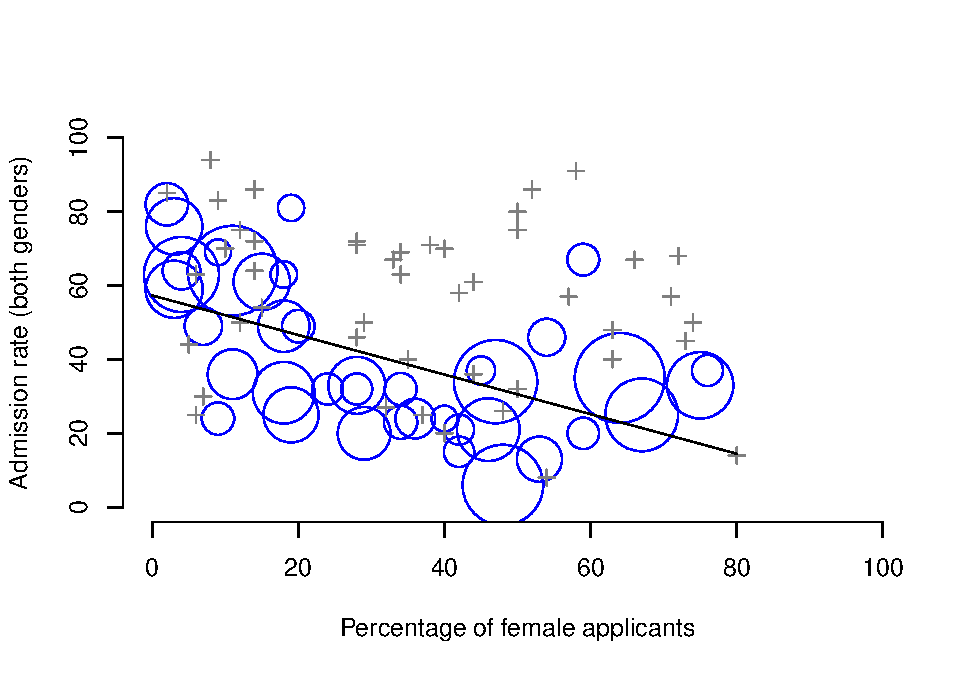
\includegraphics{lsj_files/figure-latex/berkeley-1.pdf}
\caption{\label{fig:berkeley}The Berkeley 1973 college admissions data. This figure plots the admission rate for the 85 departments that had at least one female applicant, as a function of the percentage of applicants that were female. The plot is a redrawing of Figure 1 from \protect\hyperlink{ref-Bickel1975}{Bickel et al.} (\protect\hyperlink{ref-Bickel1975}{1975}). Circles plot departments with more than 40 applicants; the area of the circle is proportional to the total number of applicants. The crosses plot department with fewer than 40 applicants.}
\end{figure}

Before leaving this topic entirely, I want to point out something else really critical that is often overlooked in a research methods class. Statistics only solves \emph{part} of the problem. Remember that we started all this with the concern that Berkeley's admissions processes might be unfairly biased against female applicants. When we looked at the ``aggregated'' data, it did seem like the university was discriminating against women, but when we ``disaggregate'' and looked at the individual behaviour of all the departments, it turned out that the actual departments were, if anything, slightly biased in favour of women. The gender bias in total admissions was caused by the fact that women tended to self-select for harder departments. From a legal perspective, that would probably put the university in the clear. Postgraduate admissions are determined at the level of the individual department, and there are good reasons to do that. At the level of individual departments the decisions are more or less unbiased (the weak bias in favour of females at that level is small, and not consistent across departments). Since the university can't dictate which departments people choose to apply to, and the decision making takes place at the level of the department it can hardly be held accountable for any biases that those choices produce.

That was the basis for my somewhat glib remarks earlier, but that's not exactly the whole story, is it? After all, if we're interested in this from a more sociological and psychological perspective, we might want to ask \emph{why} there are such strong gender differences in applications. Why do males tend to apply to engineering more often than females, and why is this reversed for the English department? And why is it the case that the departments that tend to have a female-application bias tend to have lower overall admission rates than those departments that have a male-application bias? Might this not still reflect a gender bias, even though every single department is itself unbiased? It might. Suppose, hypothetically, that males preferred to apply to ``hard sciences'' and females prefer ``humanities.'' And suppose further that the reason for why the humanities departments have low admission rates is because the government doesn't want to fund the humanities (Ph.D.~places, for instance, are often tied to government funded research projects). Does that constitute a gender bias? Or just an unenlightened view of the value of the humanities? What if someone at a high level in the government cut the humanities funds because they felt that the humanities are ``useless chick stuff.'' That seems pretty \emph{blatantly} gender biased. None of this falls within the purview of statistics, but it matters to the research project. If you're interested in the overall structural effects of subtle gender biases, then you probably want to look at \emph{both} the aggregated and disaggregated data. If you're interested in the decision making process at Berkeley itself then you're probably only interested in the disaggregated data.

In short there are a lot of critical questions that you can't answer with statistics, but the answers to those questions will have a huge impact on how you analyse and interpret data. And this is the reason why you should always think of statistics as a \emph{tool} to help you learn about your data. No more and no less. It's a powerful tool to that end, but there's no substitute for careful thought.

\hypertarget{statistics-in-psychology}{%
\section{Statistics in psychology}\label{statistics-in-psychology}}

I hope that the discussion above helped explain why science in general is so focused on statistics. But I'm guessing that you have a lot more questions about what role statistics plays in psychology, and specifically why psychology classes always devote so many lectures to stats. So here's my attempt to answer a few of them\ldots{}

\textbf{Why does psychology have so much statistics?}

To be perfectly honest, there's a few different reasons, some of which are better than others. The most important reason is that psychology is a statistical science. What I mean by that is that the ``things'' that we study are \emph{people}. Real, complicated, gloriously messy, infuriatingly perverse people. The ``things'' of physics include objects like electrons, and while there are all sorts of complexities that arise in physics, electrons don't have minds of their own. They don't have opinions, they don't differ from each other in weird and arbitrary ways, they don't get bored in the middle of an experiment, and they don't get angry at the experimenter and then deliberately try to sabotage the data set (not that I've ever done that!). At a fundamental level psychology is harder than physics.\footnote{Which might explain why physics is just a teensy bit further advanced as a science than we are.}

Basically, we teach statistics to you as psychologists because you need to be better at stats than physicists. There's actually a saying used sometimes in physics, to the effect that ``if your experiment needs statistics, you should have done a better experiment.'' They have the luxury of being able to say that because their objects of study are pathetically simple in comparison to the vast mess that confronts social scientists. And it's not just psychology. Most social sciences are desperately reliant on statistics. Not because we're bad experimenters, but because we've picked a harder problem to solve. We teach you stats because you really, really need it.

\textbf{Can't someone else do the statistics?}

To some extent, but not completely. It's true that you don't need to become a fully trained statistician just to do psychology, but you do need to reach a certain level of statistical competence. In my view, there's three reasons that every psychological researcher ought to be able to do basic statistics:

\begin{itemize}
\tightlist
\item
  Firstly, there's the fundamental reason: statistics is deeply intertwined with research design. If you want to be good at designing psychological studies, you need to at the very least understand the basics of stats.
\item
  Secondly, if you want to be good at the psychological side of the research, then you need to be able to understand the psychological literature, right? But almost every paper in the psychological literature reports the results of statistical analyses. So if you really want to understand the psychology, you need to be able to understand what other people did with their data. And that means understanding a certain amount of statistics.
\item
  Thirdly, there's a big practical problem with being dependent on other people to do all your statistics: statistical analysis is \emph{expensive}. If you ever get bored and want to look up how much the Australian government charges for university fees, you'll notice something interesting: statistics is designated as a ``national priority'' category, and so the fees are much, much lower than for any other area of study. This is because there's a massive shortage of statisticians out there. So, from your perspective as a psychological researcher, the laws of supply and demand aren't exactly on your side here! As a result, in almost any real life situation where you want to do psychological research, the cruel facts will be that you don't have enough money to afford a statistician. So the economics of the situation mean that you have to be pretty self-sufficient.
\end{itemize}

Note that a lot of these reasons generalise beyond researchers. If you want to be a practicing psychologist and stay on top of the field, it helps to be able to read the scientific literature, which relies pretty heavily on statistics.

\textbf{I don't care about jobs, research, or clinical work. Do I need statistics?}

Okay, now you're just messing with me. Still, I think it should matter to you too. Statistics should matter to you in the same way that statistics should matter to \emph{everyone}. We live in the 21st century, and data are \emph{everywhere}. Frankly, given the world in which we live these days, a basic knowledge of statistics is pretty damn close to a survival tool! Which is the topic of the next section.

\hypertarget{statistics-in-everyday-life}{%
\section{Statistics in everyday life}\label{statistics-in-everyday-life}}

~~~~~~\emph{"We are drowning in information,}\\
\hspace*{0.333em}\hspace*{0.333em}\hspace*{0.333em}\hspace*{0.333em}\hspace*{0.333em}\hspace*{0.333em}\emph{but we are starved for knowledge"}\\
\hspace*{0.333em}\hspace*{0.333em}\hspace*{0.333em}\hspace*{0.333em}\hspace*{0.333em}\hspace*{0.333em}\hspace*{0.333em}\hspace*{0.333em}\hspace*{0.333em}\hspace*{0.333em}\hspace*{0.333em}\hspace*{0.333em}\hspace*{0.333em}\hspace*{0.333em}\hspace*{0.333em}\hspace*{0.333em}\hspace*{0.333em}\hspace*{0.333em}\hspace*{0.333em}\hspace*{0.333em}\hspace*{0.333em}\hspace*{0.333em}-- Various authors, original probably John Naisbitt

\hfill\break
When I started writing up my lecture notes I took the 20 most recent news articles posted to the ABC news website. Of those 20 articles, it turned out that 8 of them involved a discussion of something that I would call a statistical topic and 6 of those made a mistake. The most common error, if you're curious, was failing to report baseline data (e.g., the article mentions that 5\% of people in situation X have some characteristic Y, but doesn't say how common the characteristic is for everyone else!). The point I'm trying to make here isn't that journalists are bad at statistics (though they almost always are), it's that a basic knowledge of statistics is very helpful for trying to figure out when someone else is either making a mistake or even lying to you. In fact, one of the biggest things that a knowledge of statistics does to you is cause you to get angry at the newspaper or the internet on a far more frequent basis. You can find a good example of this in \ref{housingpriceexample}. In later versions of this book I'll try to include more anecdotes along those lines.

\hypertarget{theres-more-to-research-methods-than-statistics}{%
\section{There's more to research methods than statistics}\label{theres-more-to-research-methods-than-statistics}}

So far, most of what I've talked about is statistics, and so you'd be forgiven for thinking that statistics is all I care about in life. To be fair, you wouldn't be far wrong, but research methodology is a broader concept than statistics. So most research methods courses will cover a lot of topics that relate much more to the pragmatics of research design, and in particular the issues that you encounter when trying to do research with humans. However, about 99\% of student \emph{fears} relate to the statistics part of the course, so I've focused on the stats in this discussion, and hopefully I've convinced you that statistics matters, and more importantly, that it's not to be feared. That being said, it's pretty typical for introductory research methods classes to be very stats-heavy. This is not (usually) because the lecturers are evil people. Quite the contrary, in fact. Introductory classes focus a lot on the statistics because you almost always find yourself needing statistics before you need the other research methods training. Why? Because almost all of your assignments in other classes will rely on statistical training, to a much greater extent than they rely on other methodological tools. It's not common for undergraduate assignments to require you to design your own study from the ground up (in which case you would need to know a lot about research design), but it \emph{is} common for assignments to ask you to analyse and interpret data that were collected in a study that someone else designed (in which case you need statistics). In that sense, from the perspective of allowing you to do well in all your other classes, the statistics is more urgent.

But note that ``urgent'' is different from ``important'' -- they both matter. I really do want to stress that research design is just as important as data analysis, and this book does spend a fair amount of time on it. However, while statistics has a kind of universality, and provides a set of core tools that are useful for most types of psychological research, the research methods side isn't quite so universal. There are some general principles that everyone should think about, but a lot of research design is very idiosyncratic, and is specific to the area of research that you want to engage in. To the extent that it's the details that matter, those details don't usually show up in an introductory stats and research methods class.

\hypertarget{studydesign}{%
\chapter{A brief introduction to research design}\label{studydesign}}

~~~~~~\emph{To consult the statistician after an experiment is finished is often merely to ask him to conduct a post mortem examination. He can perhaps say what the experiment died of.}\\
\hspace*{0.333em}\hspace*{0.333em}\hspace*{0.333em}\hspace*{0.333em}\hspace*{0.333em}\hspace*{0.333em}\hspace*{0.333em}\hspace*{0.333em}\hspace*{0.333em}\hspace*{0.333em}\hspace*{0.333em}\hspace*{0.333em}\hspace*{0.333em}\hspace*{0.333em}\hspace*{0.333em}\hspace*{0.333em}\hspace*{0.333em}\hspace*{0.333em}\hspace*{0.333em}\hspace*{0.333em}\hspace*{0.333em}\hspace*{0.333em}\hspace*{0.333em}\hspace*{0.333em}\hspace*{0.333em}\hspace*{0.333em}\hspace*{0.333em}\hspace*{0.333em}\hspace*{0.333em}\hspace*{0.333em}-- Sir Ronald Fisher\footnote{Presidential Address to the First Indian Statistical Congress, 1938. Source: \url{http://en.wikiquote.org/wiki/Ronald_Fisher}}

In this chapter, we're going to start thinking about the basic ideas that go into designing a study, collecting data, checking whether your data collection works, and so on. It won't give you enough information to allow you to design studies of your own, but it will give you a lot of the basic tools that you need to assess the studies done by other people. However, since the focus of this book is much more on data analysis than on data collection, I'm only giving a very brief overview. Note that this chapter is ``special'' in two ways. Firstly, it's much more psychology-specific than the later chapters. Secondly, it focuses much more heavily on the scientific problem of research methodology, and much less on the statistical problem of data analysis. Nevertheless, the two problems are related to one another, so it's traditional for stats textbooks to discuss the problem in a little detail. This chapter relies heavily on \protect\hyperlink{ref-Campbell1963}{Campbell \& Stanley} (\protect\hyperlink{ref-Campbell1963}{1963}) for the discussion of study design, and \protect\hyperlink{ref-Stevens1946}{Stevens} (\protect\hyperlink{ref-Stevens1946}{1946}) for the discussion of scales of measurement.

\hypertarget{measurement}{%
\section{Introduction to psychological measurement}\label{measurement}}

The first thing to understand is data collection can be thought of as a kind of {\textbf{measurement}}. That is, what we're trying to do here is measure something about human behaviour or the human mind. What do I mean by ``measurement?''

\hypertarget{some-thoughts-about-psychological-measurement}{%
\subsection{Some thoughts about psychological measurement}\label{some-thoughts-about-psychological-measurement}}

Measurement itself is a subtle concept, but basically it comes down to finding some way of assigning numbers, or labels, or some other kind of well-defined descriptions, to ``stuff.'' So, any of the following would count as a psychological measurement:

\begin{itemize}
\tightlist
\item
  My \textbf{age} is \emph{33 years}.
\item
  I \emph{do not} \textbf{like anchovies}.
\item
  My \textbf{chromosomal gender} is \emph{male}.
\item
  My \textbf{self-identified gender} is \emph{female}.
\end{itemize}

In the short list above, the \textbf{bolded part} is ``the thing to be measured,'' and the \emph{italicised part} is ``the measurement itself.'' In fact, we can expand on this a little bit, by thinking about the set of possible measurements that could have arisen in each case:

\begin{itemize}
\tightlist
\item
  My \textbf{age} (in years) could have been \emph{0, 1, 2, 3 \ldots{}}, etc. The upper bound on what my age could possibly be is a bit fuzzy, but in practice you'd be safe in saying that the largest possible age is \emph{150}, since no human has ever lived that long.
\item
  When asked if I \textbf{like anchovies}, I might have said that \emph{I do}, or \emph{I do not}, or \emph{I have no opinion}, or \emph{I sometimes do}.
\item
  My \textbf{chromosomal gender} is almost certainly going to be \emph{male (XY)} or \emph{female (XX)}, but there are a few other possibilities. I could also have \emph{Klinfelter's syndrome (XXY)}, which is more similar to male than to female. And I imagine there are other possibilities too.
\item
  My \textbf{self-identified gender} is also very likely to be \emph{male} or \emph{female}, but it doesn't have to agree with my chromosomal gender. I may also choose to identify with \emph{neither}, or to explicitly call myself \emph{transgender}.
\end{itemize}

As you can see, for some things (like age) it seems fairly obvious what the set of possible measurements should be, whereas for other things it gets a bit tricky. But I want to point out that even in the case of someone's age it's much more subtle than this. For instance, in the example above I assumed that it was okay to measure age in years. But if you're a developmental psychologist, that's way too crude, and so you often measure age in \emph{years and months} (if a child is 2 years and 11 months this is usually written as ``2;11''). If you're interested in newborns you might want to measure age in \emph{days since birth}, maybe even \emph{hours since birth}. In other words, the way in which you specify the allowable measurement values is important.

Looking at this a bit more closely, you might also realise that the concept of ``age'' isn't actually all that precise. In general, when we say ``age'' we implicitly mean ``the length of time since birth.'' But that's not always the right way to do it. Suppose you're interested in how newborn babies control their eye movements. If you're interested in kids that young, you might also start to worry that ``birth'' is not the only meaningful point in time to care about. If Baby Alice is born 3 weeks premature and Baby Bianca is born 1 week late, would it really make sense to say that they are the ``same age'' if we encountered them ``2 hours after birth?'' In one sense, yes. By social convention we use birth as our reference point for talking about age in everyday life, since it defines the amount of time the person has been operating as an independent entity in the world. But from a scientific perspective that's not the only thing we care about. When we think about the biology of human beings, it's often useful to think of ourselves as organisms that have been growing and maturing since conception, and from that perspective Alice and Bianca aren't the same age at all. So you might want to define the concept of ``age'' in two different ways: the length of time since conception and the length of time since birth. When dealing with adults it won't make much difference, but when dealing with newborns it might.

Moving beyond these issues, there's the question of methodology. What specific ``measurement method'' are you going to use to find out someone's age? As before, there are lots of different possibilities:

\begin{itemize}
\tightlist
\item
  You could just ask people ``how old are you?'' The method of self-report is fast, cheap and easy. But it only works with people old enough to understand the question, and some people lie about their age.
\item
  You could ask an authority (e.g., a parent) ``how old is your child?'' This method is fast, and when dealing with kids it's not all that hard since the parent is almost always around. It doesn't work as well if you want to know ``age since conception,'' since a lot of parents can't say for sure when conception took place. For that, you might need a different authority (e.g., an obstetrician).
\item
  You could look up official records, for example birth or death certificates. This is a time consuming and frustrating endeavour, but it has its uses (e.g., if the person is now dead).
\end{itemize}

\hypertarget{operationalisation-defining-your-measurement}{%
\subsection{Operationalisation: defining your measurement}\label{operationalisation-defining-your-measurement}}

All of the ideas discussed in the previous section relate to the concept of {\textbf{operationalisation}}. To be a bit more precise about the idea, operationalisation is the process by which we take a meaningful but somewhat vague concept and turn it into a precise measurement. The process of operationalisation can involve several different things:

\begin{itemize}
\tightlist
\item
  Being precise about what you are trying to measure. For instance, does ``age'' mean ``time since birth'' or ``time since conception'' in the context of your research?
\item
  Determining what method you will use to measure it. Will you use self-report to measure age, ask a parent, or look up an official record? If you're using self-report, how will you phrase the question?
\item
  Defining the set of allowable values that the measurement can take. Note that these values don't always have to be numerical, though they often are. When measuring age the values are numerical, but we still need to think carefully about what numbers are allowed. Do we want age in years, years and months, days, or hours? For other types of measurements (e.g., gender) the values aren't numerical. But, just as before, we need to think about what values are allowed. If we're asking people to self-report their gender, what options to we allow them to choose between? Is it enough to allow only ``male'' or ``female?'' Do you need an ``other'' option? Or should we not give people specific options and instead let them answer in their own words? And if you open up the set of possible values to include all verbal response, how will you interpret their answers?
\end{itemize}

Operationalisation is a tricky business, and there's no ``one, true way'' to do it. The way in which you choose to operationalise the informal concept of ``age'' or ``gender'' into a formal measurement depends on what you need to use the measurement for. Often you'll find that the community of scientists who work in your area have some fairly well-established ideas for how to go about it. In other words, operationalisation needs to be thought through on a case by case basis. Nevertheless, while there a lot of issues that are specific to each individual research project, there are some aspects to it that are pretty general.

Before moving on I want to take a moment to clear up our terminology, and in the process introduce one more term. Here are four different things that are closely related to each other:

\begin{itemize}
\tightlist
\item
  {\textbf{A theoretical construct}}. This is the thing that you're trying to take a measurement of, like ``age,'' ``gender'' or an ``opinion.'' A theoretical construct can't be directly observed, and often they're actually a bit vague.
\item
  {\textbf{A measure}}. The measure refers to the method or the tool that you use to make your observations. A question in a survey, a behavioural observation or a brain scan could all count as a measure.
\item
  {\textbf{An operationalisation}}. The term ``operationalisation'' refers to the logical connection between the measure and the theoretical construct, or to the process by which we try to derive a measure from a theoretical construct.
\item
  {\textbf{A variable}}. Finally, a new term. A variable is what we end up with when we apply our measure to something in the world. That is, variables are the actual ``data'' that we end up with in our data sets.
\end{itemize}

In practice, even scientists tend to blur the distinction between these things, but it's very helpful to try to understand the differences.

\hypertarget{scales}{%
\section{Scales of measurement}\label{scales}}

As the previous section indicates, the outcome of a psychological measurement is called a variable. But not all variables are of the same qualitative type and so it's useful to understand what types there are. A very useful concept for distinguishing between different types of variables is what's known as {\textbf{scales of measurement}}.

\hypertarget{nominal-scale}{%
\subsection{Nominal scale}\label{nominal-scale}}

A {\textbf{nominal scale}} variable (also referred to as a {\textbf{categorical}} variable) is one in which there is no particular relationship between the different possibilities. For these kinds of variables it doesn't make any sense to say that one of them is ``bigger' or''better" than any other one, and it absolutely doesn't make any sense to average them. The classic example for this is ``eye colour.'' Eyes can be blue, green or brown, amongst other possibilities, but none of them is any ``bigger'' than any other one. As a result, it would feel really weird to talk about an ``average eye colour.'' Similarly, gender is nominal too: male isn't better or worse than female, non-binary, or any other gender a person identifies as Neither does it make sense to try to talk about an ``average gender.'' In short, nominal scale variables are those for which the only thing you can say about the different possibilities is that they are different. That's it.

Let's take a slightly closer look at this. Suppose I was doing research on how people commute to and from work. One variable I would have to measure would be what kind of transportation people use to get to work. This ``transport type'' variable could have quite a few possible values, including: ``train,'' ``bus,'' ``car,'' ``bicycle.'' For now, let's suppose that these four are the only possibilities. Then imagine that I ask 100 people how they got to work today, with this result:

\begin{longtable}[]{@{}lc@{}}
\toprule
Transportation & Number of people\tabularnewline
\midrule
\endhead
(1) Train & 12\tabularnewline
(2) Bus & 30\tabularnewline
(3) Car & 48\tabularnewline
(4) Bicycle & 10\tabularnewline
\bottomrule
\end{longtable}

So, what's the average transportation type? Obviously, the answer here is that there isn't one. It's a silly question to ask. You can say that travel by car is the most popular method, and travel by train is the least popular method, but that's about all. Similarly, notice that the order in which I list the options isn't very interesting. I could have chosen to display the data like this

\begin{longtable}[]{@{}lc@{}}
\toprule
Transportation & Number of people\tabularnewline
\midrule
\endhead
(3) Car & 48\tabularnewline
(1) Train & 12\tabularnewline
(4) Bicycle & 10\tabularnewline
(2) Bus & 30\tabularnewline
\bottomrule
\end{longtable}

and nothing really changes.

\hypertarget{ordinal-scale}{%
\subsection{Ordinal scale}\label{ordinal-scale}}

{\textbf{Ordinal scale}} variables have a bit more structure than nominal scale variables, but not by a lot. An ordinal scale variable is one in which there is a natural, meaningful way to order the different possibilities, but you can't do anything else. The usual example given of an ordinal variable is ``finishing position in a race.'' You \emph{can} say that the person who finished first was faster than the person who finished second, but you \emph{don't} know how much faster. As a consequence we know that 1st \(>\) 2nd, and we know that 2nd \(>\) 3rd, but the difference between 1st and 2nd might be much larger than the difference between 2nd and 3rd.

Here's a more psychologically interesting example. Suppose I'm interested in people's attitudes to climate change. I then go and ask some people to pick the statement (from four listed statements) that most closely matches their beliefs:

~~(1) Temperatures are rising because of human activity\\
\hspace*{0.333em}\hspace*{0.333em}(2) Temperatures are rising but we don't know why\\
\hspace*{0.333em}\hspace*{0.333em}(3) Temperatures are rising but not because of humans\\
\hspace*{0.333em}\hspace*{0.333em}(4) Temperatures are not rising

\hfill\break
Notice that these four statements actually do have a natural ordering, in terms of ``the extent to which they agree with the current science.'' Statement 1 is a close match, statement 2 is a reasonable match, statement 3 isn't a very good match, and statement 4 is in strong opposition to current science. So, in terms of the thing I'm interested in (the extent to which people endorse the science), I can order the items as \(1 > 2 > 3 > 4\). Since this ordering exists, it would be very weird to list the options like this

~~(3) Temperatures are rising but not because of humans\\
\hspace*{0.333em}\hspace*{0.333em}(1) Temperatures are rising because of human activity\\
\hspace*{0.333em}\hspace*{0.333em}(4) Temperatures are not rising\\
\hspace*{0.333em}\hspace*{0.333em}(2) Temperatures are rising but we don't know why

\hfill\break
because it seems to violate the natural ``structure'' to the question.

So, let's suppose I asked 100 people these questions, and got the following answers

\begin{longtable}[]{@{}lc@{}}
\toprule
Response & Number\tabularnewline
\midrule
\endhead
(1) Temperatures are rising, because of human activity & 51\tabularnewline
(2) Temperatures are rising, but we don't know why & 20\tabularnewline
(3) Temperatures are rising, but not because of humans & 10\tabularnewline
(4) Temperatures are not rising & 19\tabularnewline
\bottomrule
\end{longtable}

\hfill\break
When analysing these data it seems quite reasonable to try to group (1), (2) and (3) together, and say that 81 out of 100 people were willing to \emph{at least partially} endorse the science. And it's \emph{also} quite reasonable to group (2), (3) and (4) together and say that 49 out of 100 people registered \emph{at least some disagreement} with the dominant scientific view. However, it would be entirely bizarre to try to group (1), (2) and (4) together and say that 90 out of 100 people said \ldots{} what? There's nothing sensible that allows you to group those responses together at all.

That said, notice that while we \emph{can} use the natural ordering of these items to construct sensible groupings, what we \emph{can't} do is average them. For instance, in my simple example here, the ``average'' response to the question is 1.97. If you can tell me what that means I'd love to know, because it seems like gibberish to me!

\hypertarget{interval-scale}{%
\subsection{Interval scale}\label{interval-scale}}

In contrast to nominal and ordinal scale variables, {\textbf{interval scale}} and ratio scale variables are variables for which the numerical value is genuinely meaningful. In the case of interval scale variables the \emph{differences} between the numbers are interpretable, but the variable doesn't have a ``natural'' zero value. A good example of an interval scale variable is measuring temperature in degrees celsius. For instance, if it was 15\(^\circ\) yesterday and 18\(^\circ\) today, then the 3\(^\circ\) difference between the two is genuinely meaningful. Moreover, that 3\(^\circ\) difference is \emph{exactly the same} as the 3\(^\circ\) difference between \(7^\circ\) and \(10^\circ\). In short, addition and subtraction are meaningful for interval scale variables.\footnote{Actually, I've been informed by readers with greater physics knowledge than I that temperature isn't strictly an interval scale, in the sense that the amount of energy required to heat something up by 3\(^\circ\) depends on it's current temperature. So in the sense that physicists care about, temperature isn't actually an interval scale. But it still makes a cute example so I'm going to ignore this little inconvenient truth.}

However, notice that the \(0^\circ\) does not mean ``no temperature at all.'' It actually means ``the temperature at which water freezes,'' which is pretty arbitrary. As a consequence it becomes pointless to try to multiply and divide temperatures. It is wrong to say that \(20^\circ\) is \emph{twice as hot} as \(10^\circ\), just as it is weird and meaningless to try to claim that \(20^\circ\) is negative two times as hot as \(-10^\circ\).

Again, lets look at a more psychological example. Suppose I'm interested in looking at how the attitudes of first-year university students have changed over time. Obviously, I'm going to want to record the year in which each student started. This is an interval scale variable. A student who started in 2003 did arrive 5 years before a student who started in 2008. However, it would be completely daft for me to divide 2008 by 2003 and say that the second student started ``1.0024 times later'' than the first one. That doesn't make any sense at all.

\hypertarget{ratio-scale}{%
\subsection{Ratio scale}\label{ratio-scale}}

The fourth and final type of variable to consider is a {\textbf{ratio scale}} variable, in which zero really means zero, and it's okay to multiply and divide. A good psychological example of a ratio scale variable is response time (RT). In a lot of tasks it's very common to record the amount of time somebody takes to solve a problem or answer a question, because it's an indicator of how difficult the task is. Suppose that Alan takes 2.3 seconds to respond to a question, whereas Ben takes 3.1 seconds. As with an interval scale variable, addition and subtraction are both meaningful here. Ben really did take \(3.1 - 2.3 = 0.8\) seconds longer than Alan did. However, notice that multiplication and division also make sense here too: Ben took \(3.1 / 2.3 = 1.35\) times as long as Alan did to answer the question. And the reason why you can do this is that for a ratio scale variable such as RT ``zero seconds'' really does mean ``no time at all.''

\hypertarget{continuousdiscrete}{%
\subsection{Continuous versus discrete variables}\label{continuousdiscrete}}

There's a second kind of distinction that you need to be aware of, regarding what types of variables you can run into. This is the distinction between continuous variables and discrete variables. The difference between these is as follows:

\begin{itemize}
\tightlist
\item
  A {\textbf{continuous variable}} is one in which, for any two values that you can think of, it's always logically possible to have another value in between.
\item
  A {\textbf{discrete variable}} is, in effect, a variable that isn't continuous. For a discrete variable it's sometimes the case that there's nothing in the middle.
\end{itemize}

These definitions probably seem a bit abstract, but they're pretty simple once you see some examples. For instance, response time is continuous. If Alan takes 3.1 seconds and Ben takes 2.3 seconds to respond to a question, then Cameron's response time will lie in between if he took 3.0 seconds. And of course it would also be possible for David to take 3.031 seconds to respond, meaning that his RT would lie in between Cameron's and Alan's. And while in practice it might be impossible to measure RT that precisely, it's certainly possible in principle. Because we can always find a new value for RT in between any two other ones we regard RT as a continuous measure.

Discrete variables occur when this rule is violated. For example, nominal scale variables are always discrete. There isn't a type of transportation that falls ``in between'' trains and bicycles, not in the strict mathematical way that 2.3 falls in between 2 and 3. So transportation type is discrete. Similarly, ordinal scale variables are always discrete. Although ``2nd place'' does fall between ``1st place'' and ``3rd place,'' there's nothing that can logically fall in between ``1st place'' and ``2nd place.'' Interval scale and ratio scale variables can go either way. As we saw above, response time (a ratio scale variable) is continuous. Temperature in degrees celsius (an interval scale variable) is also continuous. However, the year you went to school (an interval scale variable) is discrete. There's no year in between 2002 and 2003. The number of questions you get right on a true-or-false test (a ratio scale variable) is also discrete. Since a true-or-false question doesn't allow you to be ``partially correct,'' there's nothing in between 5/10 and 6/10. Table \ref{tab:scalescont} summarises the relationship between the scales of measurement and the discrete/continuity distinction. Cells with a tick mark correspond to things that are possible. I'm trying to hammer this point home, because (a) some textbooks get this wrong, and (b) people very often say things like ``discrete variable'' when they mean ``nominal scale variable.'' It's very unfortunate.

\begin{table}

\caption{\label{tab:scalescont}The relationship between the scales of measurement and the discrete/continuity distinction. Cells with a tick mark correspond to things that are possible.}
\centering
\begin{tabular}[t]{lcc}
\toprule
 & continuous & discrete\\
\midrule
nominal &  & \$\textbackslash{}checkmark\$\\
ordinal &  & \$\textbackslash{}checkmark\$\\
interval & \$\textbackslash{}checkmark\$ & \$\textbackslash{}checkmark\$\\
ratio & \$\textbackslash{}checkmark\$ & \$\textbackslash{}checkmark\$\\
\bottomrule
\end{tabular}
\end{table}

\hypertarget{some-complexities}{%
\subsection{Some complexities}\label{some-complexities}}

Okay, I know you're going to be shocked to hear this, but the real world is much messier than this little classification scheme suggests. Very few variables in real life actually fall into these nice neat categories, so you need to be kind of careful not to treat the scales of measurement as if they were hard and fast rules. It doesn't work like that. They're guidelines, intended to help you think about the situations in which you should treat different variables differently. Nothing more.

So let's take a classic example, maybe \emph{the} classic example, of a psychological measurement tool: the {\textbf{Likert scale}}. The humble Likert scale is the bread and butter tool of all survey design. You yourself have filled out hundreds, maybe thousands, of them and odds are you've even used one yourself. Suppose we have a survey question that looks like this:

``Which of the following best describes your opinion of the statement that''all pirates are freaking awesome``?''

\hfill\break
and then the options presented to the participant are these:

\begin{enumerate}
\def\labelenumi{(\arabic{enumi})}
\tightlist
\item
  Strongly disagree
\item
  Disagree
\item
  Neither agree nor disagree
\item
  Agree
\item
  Strongly agree
\end{enumerate}

This set of items is an example of a 5-point Likert scale, in which people are asked to choose among one of several (in this case 5) clearly ordered possibilities, generally with a verbal descriptor given in each case. However, it's not necessary that all items are explicitly described. This is a perfectly good example of a 5-point Likert scale too:

\begin{enumerate}
\def\labelenumi{(\arabic{enumi})}
\tightlist
\item
  Strongly disagree
\item
\item
\item
\item
  Strongly agree
\end{enumerate}

Likert scales are very handy, if somewhat limited, tools. The question is what kind of variable are they? They're obviously discrete, since you can't give a response of 2.5. They're obviously not nominal scale, since the items are ordered; and they're not ratio scale either, since there's no natural zero.

But are they ordinal scale or interval scale? One argument says that we can't really prove that the difference between ``strongly agree'' and ``agree'' is of the same size as the difference between ``agree'' and ``neither agree nor disagree.'' In fact, in everyday life it's pretty obvious that they're not the same at all. So this suggests that we ought to treat Likert scales as ordinal variables. On the other hand, in practice most participants do seem to take the whole ``on a scale from 1 to 5'' part fairly seriously, and they tend to act as if the differences between the five response options were fairly similar to one another. As a consequence, a lot of researchers treat Likert scale data as interval scale.\footnote{Ah, psychology \ldots{} never an easy answer to anything!} It's not interval scale, but in practice it's close enough that we usually think of it as being {\textbf{quasi-interval scale}}.

\hypertarget{reliability}{%
\section{Assessing the reliability of a measurement}\label{reliability}}

At this point we've thought a little bit about how to operationalise a theoretical construct and thereby create a psychological measure. And we've seen that by applying psychological measures we end up with variables, which can come in many different types. At this point, we should start discussing the obvious question: is the measurement any good? We'll do this in terms of two related ideas: \emph{reliability} and \emph{validity}. Put simply, the {\textbf{reliability}} of a measure tells you how \emph{precisely} you are measuring something, whereas the validity of a measure tells you how \emph{accurate} the measure is. In this section I'll talk about reliability; we'll talk about validity in section \ref{validity}.

Reliability is actually a very simple concept. It refers to the repeatability or consistency of your measurement. The measurement of my weight by means of a ``bathroom scale'' is very reliable. If I step on and off the scales over and over again, it'll keep giving me the same answer. Measuring my intelligence by means of ``asking my mum'' is very unreliable. Some days she tells me I'm a bit thick, and other days she tells me I'm a complete idiot. Notice that this concept of reliability is different to the question of whether the measurements are correct (the correctness of a measurement relates to it's validity). If I'm holding a sack of potatos when I step on and off the bathroom scales the measurement will still be reliable: it will always give me the same answer. However, this highly reliable answer doesn't match up to my true weight at all, therefore it's wrong. In technical terms, this is a \emph{reliable but invalid} measurement. Similarly, whilst my mum's estimate of my intelligence is a bit unreliable, she might be right. Maybe I'm just not too bright, and so while her estimate of my intelligence fluctuates pretty wildly from day to day, it's basically right. That would be an \emph{unreliable but valid} measure. Of course, if my mum's estimates are too unreliable it's going to be very hard to figure out which one of her many claims about my intelligence is actually the right one. To some extent, then, a very unreliable measure tends to end up being invalid for practical purposes; so much so that many people would say that reliability is necessary (but not sufficient) to ensure validity.

Okay, now that we're clear on the distinction between reliability and validity, let's have a think about the different ways in which we might measure reliability:

\begin{itemize}
\tightlist
\item
  {\textbf{Test-retest reliability}}. This relates to consistency over time. If we repeat the measurement at a later date do we get a the same answer?
\item
  {\textbf{Inter-rater reliability}}. This relates to consistency across people. If someone else repeats the measurement (e.g., someone else rates my intelligence) will they produce the same answer?
\item
  {\textbf{Parallel forms reliability}}. This relates to consistency across theoretically-equivalent measurements. If I use a different set of bathroom scales to measure my weight does it give the same answer?
\item
  {\textbf{Internal consistency reliability}}. If a measurement is constructed from lots of different parts that perform similar functions (e.g., a personality questionnaire result is added up across several questions) do the individual parts tend to give similar answers. We'll look at this particular form of reliability later in the book, in Section \ref{rel}.
\end{itemize}

Not all measurements need to possess all forms of reliability. For instance, educational assessment can be thought of as a form of measurement. One of the subjects that I teach, \emph{Computational Cognitive Science}, has an assessment structure that has a research component and an exam component (plus other things). The exam component is \emph{intended} to measure something different from the research component, so the assessment as a whole has low internal consistency. However, within the exam there are several questions that are intended to (approximately) measure the same things, and those tend to produce similar outcomes. So the exam on its own has a fairly high internal consistency. Which is as it should be. You should only demand reliability in those situations where you want to be measuring the same thing!

\hypertarget{ivdv}{%
\section{The ``role'' of variables: predictors and outcomes}\label{ivdv}}

I've got one last piece of terminology that I need to explain to you before moving away from variables. Normally, when we do some research we end up with lots of different variables. Then, when we analyse our data, we usually try to explain some of the variables in terms of some of the other variables. It's important to keep the two roles ``thing doing the explaining'' and ``thing being explained'' distinct. So let's be clear about this now. First, we might as well get used to the idea of using mathematical symbols to describe variables, since it's going to happen over and over again. Let's denote the ``to be explained'' variable \(Y\), and denote the variables ``doing the explaining'' as \(X_1\), \(X_2\), etc.

When we are doing an analysis we have different names for \(X\) and \(Y\), since they play different roles in the analysis. The classical names for these roles are {\textbf{independent variable}} (IV) and {\textbf{dependent variable}} (DV). The IV is the variable that you use to do the explaining (i.e., \(X\)) and the DV is the variable being explained (i.e., \(Y\)). The logic behind these names goes like this: if there really is a relationship between \(X\) and \(Y\) then we can say that \(Y\) depends on \(X\), and if we have designed our study ``properly'' then \(X\) isn't dependent on anything else. However, I personally find those names horrible. They're hard to remember and they're highly misleading because (a) the IV is never actually ``independent of everything else,'' and (b) if there's no relationship then the DV doesn't actually depend on the IV. And in fact, because I'm not the only person who thinks that IV and DV are just awful names, there are a number of alternatives that I find more appealing. The terms that I'll use in this book are {\textbf{predictors}} and {\textbf{outcomes}}. The idea here is that what you're trying to do is use \(X\) (the predictors) to make guesses about \(Y\) (the outcomes).\footnote{Annoyingly though, there's a lot of different names used out there. I won't list all of them -- there would be no point in doing that -- other than to note that ``response variable'' is sometimes used where I've used ``outcome.'' Sigh. This sort of terminological confusion is very common, I'm afraid.} This is summarised in Table \ref{tab:ivdv}.

\begin{table}

\caption{\label{tab:ivdv}The terminology used to distinguish between different roles that a variable can play when analysing a data set. Note that this book will tend to avoid the classical terminology in favour of the newer names.}
\centering
\begin{tabular}[t]{lll}
\toprule
role of the variable & classical name & modern name\\
\midrule
"to be explained" & dependent variable (DV) & outcome\\
"to do the explaining" & independent variable (IV) & predictor\\
\bottomrule
\end{tabular}
\end{table}

\hypertarget{researchdesigns}{%
\section{Experimental and non-experimental research}\label{researchdesigns}}

One of the big distinctions that you should be aware of is the distinction between ``experimental research'' and ``non-experimental research.'' When we make this distinction, what we're really talking about is the degree of control that the researcher exercises over the people and events in the study.

\hypertarget{experimental-research}{%
\subsection{Experimental research}\label{experimental-research}}

The key feature of {\textbf{experimental research}} is that the researcher controls all aspects of the study, especially what participants experience during the study. In particular, the researcher manipulates or varies the predictor variables (IVs) but allows the outcome variable (DV) to vary naturally. The idea here is to deliberately vary the predictors (IVs) to see if they have any causal effects on the outcomes. Moreover, in order to ensure that there's no possibility that something other than the predictor variables is causing the outcomes, everything else is kept constant or is in some other way ``balanced,'' to ensure that they have no effect on the results. In practice, it's almost impossible to \emph{think} of everything else that might have an influence on the outcome of an experiment, much less keep it constant. The standard solution to this is {\textbf{randomisation}}. That is, we randomly assign people to different groups, and then give each group a different treatment (i.e., assign them different values of the predictor variables). We'll talk more about randomisation later, but for now it's enough to say that what randomisation does is minimise (but not eliminate) the possibility that there are any systematic difference between groups.

Let's consider a very simple, completely unrealistic and grossly unethical example. Suppose you wanted to find out if smoking causes lung cancer. One way to do this would be to find people who smoke and people who don't smoke and look to see if smokers have a higher rate of lung cancer. This is \emph{not} a proper experiment, since the researcher doesn't have a lot of control over who is and isn't a smoker. And this really matters. For instance, it might be that people who choose to smoke cigarettes also tend to have poor diets, or maybe they tend to work in asbestos mines, or whatever. The point here is that the groups (smokers and non-smokers) actually differ on lots of things, not \emph{just} smoking. So it might be that the higher incidence of lung cancer among smokers is caused by something else, and not by smoking per se. In technical terms these other things (e.g.~diet) are called ``confounders,'' and we'll talk about those in just a moment.

In the meantime, let's consider what a proper experiment might look like. Recall that our concern was that smokers and non-smokers might differ in lots of ways. The solution, as long as you have no ethics, is to \emph{control} who smokes and who doesn't. Specifically, if we randomly divide young non-smokers into two groups and force half of them to become smokers, then it's very unlikely that the groups will differ in any respect other than the fact that half of them smoke. That way, if our smoking group gets cancer at a higher rate than the non-smoking group, we can feel pretty confident that (a) smoking does cause cancer and (b) we're murderers.

\hypertarget{non-experimental-research}{%
\subsection{Non-experimental research}\label{non-experimental-research}}

{\textbf{Non-experimental research}} is a broad term that covers ``any study in which the researcher doesn't have as much control as they do in an experiment.'' Obviously, control is something that scientists like to have, but as the previous example illustrates there are lots of situations in which you can't or shouldn't try to obtain that control. Since it's grossly unethical (and almost certainly criminal) to force people to smoke in order to find out if they get cancer, this is a good example of a situation in which you really shouldn't try to obtain experimental control. But there are other reasons too. Even leaving aside the ethical issues, our ``smoking experiment'' does have a few other issues. For instance, when I suggested that we ``force'' half of the people to become smokers, I was talking about \emph{starting} with a sample of non-smokers, and then forcing them to become smokers. While this sounds like the kind of solid, evil experimental design that a mad scientist would love, it might not be a very sound way of investigating the effect in the real world. For instance, suppose that smoking only causes lung cancer when people have poor diets, and suppose also that people who normally smoke do tend to have poor diets. However, since the ``smokers'' in our experiment aren't ``natural'' smokers (i.e., we forced non-smokers to become smokers, but they didn't take on all of the other normal, real life characteristics that smokers might tend to possess) they probably have better diets. As such, in this silly example they wouldn't get lung cancer and our experiment will fail, because it violates the structure of the ``natural'' world (the technical name for this is an ``artefactual'' result).

One distinction worth making between two types of non-experimental research is the difference between {\textbf{quasi-experimental research}} and {\textbf{case studies}}. The example I discussed earlier, in which we wanted to examine incidence of lung cancer among smokers and non-smokers without trying to control who smokes and who doesn't, is a quasi-experimental design. That is, it's the same as an experiment but we don't control the predictors (IVs). We can still use statistics to analyse the results, but we have to be a lot more careful and circumspect.

The alternative approach, case studies, aims to provide a very detailed description of one or a few instances. In general, you can't use statistics to analyse the results of case studies and it's usually very hard to draw any general conclusions about ``people in general'' from a few isolated examples. However, case studies are very useful in some situations. Firstly, there are situations where you don't have any alternative. Neuropsychology has this issue a lot. Sometimes, you just can't find a lot of people with brain damage in a specific brain area, so the only thing you can do is describe those cases that you do have in as much detail and with as much care as you can. However, there's also some genuine advantages to case studies. Because you don't have as many people to study you have the ability to invest lots of time and effort trying to understand the specific factors at play in each case. This is a very valuable thing to do. As a consequence, case studies can complement the more statistically-oriented approaches that you see in experimental and quasi-experimental designs. We won't talk much about case studies in this book, but they are nevertheless very valuable tools!

\hypertarget{validity}{%
\section{Assessing the validity of a study}\label{validity}}

More than any other thing, a scientist wants their research to be ``valid.'' The conceptual idea behind {\textbf{validity}} is very simple. Can you trust the results of your study? If not, the study is invalid. However, whilst it's easy to state, in practice it's much harder to check validity than it is to check reliability. And in all honesty, there's no precise, clearly agreed upon notion of what validity actually is. In fact, there are lots of different kinds of validity, each of which raises it's own issues. And not all forms of validity are relevant to all studies. I'm going to talk about five different types of validity:

\begin{itemize}
\tightlist
\item
  Internal validity
\item
  External validity
\item
  Construct validity
\item
  Face validity
\item
  Ecological validity
\end{itemize}

First, a quick guide as to what matters here. (1) Internal and external validity are the most important, since they tie directly to the fundamental question of whether your study really works. (2) Construct validity asks whether you're measuring what you think you are. (3) Face validity isn't terribly important except insofar as you care about ``appearances.'' (4) Ecological validity is a special case of face validity that corresponds to a kind of appearance that you might care about a lot.

\hypertarget{internal-validity}{%
\subsection{Internal validity}\label{internal-validity}}

{\textbf{Internal validity}} refers to the extent to which you are able draw the correct conclusions about the causal relationships between variables. It's called ``internal'' because it refers to the relationships between things ``inside'' the study. Let's illustrate the concept with a simple example. Suppose you're interested in finding out whether a university education makes you write better. To do so, you get a group of first year students, ask them to write a 1000 word essay, and count the number of spelling and grammatical errors they make. Then you find some third-year students, who obviously have had more of a university education than the first-years, and repeat the exercise. And let's suppose it turns out that the third-year students produce fewer errors. And so you conclude that a university education improves writing skills. Right? Except that the big problem with this experiment is that the third-year students are older and they've had more experience with writing things. So it's hard to know for sure what the causal relationship is. Do older people write better? Or people who have had more writing experience? Or people who have had more education? Which of the above is the true \emph{cause} of the superior performance of the third-years? Age? Experience? Education? You can't tell. This is an example of a failure of internal validity, because your study doesn't properly tease apart the \emph{causal} relationships between the different variables.

\hypertarget{external-validity}{%
\subsection{External validity}\label{external-validity}}

{\textbf{External validity}} relates to the {\textbf{generalisability}} or {\textbf{applicability}} of your findings. That is, to what extent do you expect to see the same pattern of results in ``real life'' as you saw in your study. To put it a bit more precisely, any study that you do in psychology will involve a fairly specific set of questions or tasks, will occur in a specific environment, and will involve participants that are drawn from a particular subgroup (disappointingly often it is college students!). So, if it turns out that the results don't actually generalise or apply to people and situations beyond the ones that you studied, then what you've got is a lack of external validity.

The classic example of this issue is the fact that a very large proportion of studies in psychology will use undergraduate psychology students as the participants. Obviously, however, the researchers don't care \emph{only} about psychology students. They care about people in general. Given that, a study that uses only psychology students as participants always carries a risk of lacking external validity. That is, if there's something ``special'' about psychology students that makes them different to the general population in some \emph{relevant} respect, then we may start worrying about a lack of external validity.

That said, it is absolutely critical to realise that a study that uses only psychology students does not necessarily have a problem with external validity. I'll talk about this again later, but it's such a common mistake that I'm going to mention it here. The external validity of a study is threatened by the choice of population if (a) the population from which you sample your participants is very narrow (e.g., psychology students), and (b) the narrow population that you sampled from is systematically different from the general population \emph{in some respect that is relevant to the psychological phenomenon that you intend to study}. The italicised part is the bit that lots of people forget. It is true that psychology undergraduates differ from the general population in lots of ways, and so a study that uses only psychology students \emph{may} have problems with external validity. However, if those differences aren't very relevant to the phenomenon that you're studying, then there's nothing to worry about. To make this a bit more concrete here are two extreme examples:

\begin{itemize}
\tightlist
\item
  You want to measure ``attitudes of the general public towards psychotherapy,'' but all of your participants are psychology students. This study would almost certainly have a problem with external validity.
\item
  You want to measure the effectiveness of a visual illusion, and your participants are all psychology students. This study is unlikely to have a problem with external validity
\end{itemize}

Having just spent the last couple of paragraphs focusing on the choice of participants, since that's a big issue that everyone tends to worry most about, it's worth remembering that external validity is a broader concept. The following are also examples of things that might pose a threat to external validity, depending on what kind of study you're doing:

\begin{itemize}
\tightlist
\item
  People might answer a ``psychology questionnaire'' in a manner that doesn't reflect what they would do in real life.
\item
  Your lab experiment on (say) ``human learning'' has a different structure to the learning problems people face in real life.
\end{itemize}

\hypertarget{construct-validity}{%
\subsection{Construct validity}\label{construct-validity}}

{\textbf{Construct validity}} is basically a question of whether you're measuring what you want to be measuring. A measurement has good construct validity if it is actually measuring the correct theoretical construct, and bad construct validity if it doesn't. To give a very simple (if ridiculous) example, suppose I'm trying to investigate the rates with which university students cheat on their exams. And the way I attempt to measure it is by asking the cheating students to stand up in the lecture theatre so that I can count them. When I do this with a class of 300 students 0 people claim to be cheaters. So I therefore conclude that the proportion of cheaters in my class is 0\%. Clearly this is a bit ridiculous. But the point here is not that this is a very deep methodological example, but rather to explain what construct validity is. The problem with my measure is that while I'm \emph{trying} to measure ``the proportion of people who cheat'' what I'm actually measuring is ``the proportion of people stupid enough to own up to cheating, or bloody minded enough to pretend that they do.'' Obviously, these aren't the same thing! So my study has gone wrong, because my measurement has very poor construct validity.

\hypertarget{face-validity}{%
\subsection{Face validity}\label{face-validity}}

{\textbf{Face validity}} simply refers to whether or not a measure ``looks like'' it's doing what it's supposed to, nothing more. If I design a test of intelligence, and people look at it and they say ``no, that test doesn't measure intelligence,'' then the measure lacks face validity. It's as simple as that. Obviously, face validity isn't very important from a pure scientific perspective. After all, what we care about is whether or not the measure \emph{actually} does what it's supposed to do, not whether it \emph{looks like} it does what it's supposed to do. As a consequence, we generally don't care very much about face validity. That said, the concept of face validity serves three useful pragmatic purposes:

\begin{itemize}
\tightlist
\item
  Sometimes, an experienced scientist will have a ``hunch'' that a particular measure won't work. While these sorts of hunches have no strict evidentiary value, it's often worth paying attention to them. Because often times people have knowledge that they can't quite verbalise, so there might be something to worry about even if you can't quite say why. In other words, when someone you trust criticises the face validity of your study, it's worth taking the time to think more carefully about your design to see if you can think of reasons why it might go awry. Mind you, if you don't find any reason for concern, then you should probably not worry. After all, face validity really doesn't matter very much.
\item
  Often (very often), completely uninformed people will also have a ``hunch'' that your research is crap. And they'll criticise it on the internet or something. On close inspection you may notice that these criticisms are actually focused entirely on how the study ``looks,'' but not on anything deeper. The concept of face validity is useful for gently explaining to people that they need to substantiate their arguments further.
\item
  Expanding on the last point, if the beliefs of untrained people are critical (e.g., this is often the case for applied research where you actually want to convince policy makers of something or other) then you \emph{have} to care about face validity. Simply because, whether you like it or not, a lot of people will use face validity as a proxy for real validity. If you want the government to change a law on scientific psychological grounds, then it won't matter how good your studies ``really'' are. If they lack face validity you'll find that politicians ignore you. Of course, it's somewhat unfair that policy often depends more on appearance than fact, but that's how things go.
\end{itemize}

\hypertarget{ecological-validity}{%
\subsection{Ecological validity}\label{ecological-validity}}

{\textbf{Ecological validity}} is a different notion of validity, which is similar to external validity, but less important. The idea is that, in order to be ecologically valid, the entire set up of the study should closely approximate the real world scenario that is being investigated. In a sense, ecological validity is a kind of face validity. It relates mostly to whether the study ``looks'' right, but with a bit more rigour to it. To be ecologically valid the study has to look right in a fairly specific way. The idea behind it is the intuition that a study that is ecologically valid is more likely to be externally valid. It's no guarantee, of course. But the nice thing about ecological validity is that it's much easier to check whether a study is ecologically valid than it is to check whether a study is externally valid. A simple example would be eyewitness identification studies. Most of these studies tend to be done in a university setting, often with a fairly simple array of faces to look at, rather than a line up. The length of time between seeing the ``criminal'' and being asked to identify the suspect in the ``line up'' is usually shorter. The ``crime'' isn't real so there's no chance of the witness being scared, and there are no police officers present so there's not as much chance of feeling pressured. These things all mean that the study \emph{definitely} lacks ecological validity. They might (but might not) mean that it also lacks external validity.

\hypertarget{confounds-artifacts-and-other-threats-to-validity}{%
\section{Confounds, artifacts and other threats to validity}\label{confounds-artifacts-and-other-threats-to-validity}}

If we look at the issue of validity in the most general fashion the two biggest worries that we have are \emph{confounders} and \emph{artefacts}. These two terms are defined in the following way:

\begin{itemize}
\tightlist
\item
  {\textbf{Confounder}}: A confounder is an additional, often unmeasured variable\footnote{The reason why I say that it's unmeasured is that if you \emph{have} measured it, then you can use some fancy statistical tricks to deal with the confounder. Because of the existence of these statistical solutions to the problem of confounders, we often refer to a confounder that we have measured and dealt with as a \emph{covariate}. Dealing with covariates is a more advanced topic, but I thought I'd mention it in passing since it's kind of comforting to at least know that this stuff exists.} that turns out to be related to both the predictors and the outcome. The existence of confounders threatens the internal validity of the study because you can't tell whether the predictor causes the outcome, or if the confounding variable causes it.
\item
  {\textbf{Artefact}}: A result is said to be ``artefactual'' if it only holds in the special situation that you happened to test in your study. The possibility that your result is an artefact describes a threat to your external validity, because it raises the possibility that you can't generalise or apply your results to the actual population that you care about.
\end{itemize}

As a general rule confounders are a bigger concern for non-experimental studies, precisely because they're not proper experiments. By definition, you're leaving lots of things uncontrolled, so there's a lot of scope for confounders being present in your study. Experimental research tends to be much less vulnerable to confounders. The more control you have over what happens during the study, the more you can prevent confounders from affecting the results. With random allocation, for example, confounders are distributed randomly, and evenly, between different groups.

However, there are always swings and roundabouts and when we start thinking about artefacts rather than confounders the shoe is very firmly on the other foot. For the most part, artefactual results tend to be a concern for experimental studies than for non-experimental studies. To see this, it helps to realise that the reason that a lot of studies are non-experimental is precisely because what the researcher is trying to do is examine human behaviour in a more naturalistic context. By working in a more real-world context you lose experimental control (making yourself vulnerable to confounders), but because you tend to be studying human psychology ``in the wild'' you reduce the chances of getting an artefactual result. Or, to put it another way, when you take psychology out of the wild and bring it into the lab (which we usually have to do to gain our experimental control), you always run the risk of accidentally studying something different to what you wanted to study.

Be warned though. The above is a rough guide only. It's absolutely possible to have confounders in an experiment, and to get artefactual results with non-experimental studies. This can happen for all sorts of reasons, not least of which is experimenter or researcher error. In practice, it's really hard to think everything through ahead of time and even very good researchers make mistakes.

Although there's a sense in which almost any threat to validity can be characterised as a confounder or an artefact, they're pretty vague concepts. So let's have a look at some of the most common examples.

\hypertarget{history-effects}{%
\subsection{History effects}\label{history-effects}}

{\textbf{History effects}} refer to the possibility that specific events may occur during the study that might influence the outcome measure. For instance, something might happen in between a pre-test and a post-test. Or in-between testing participant 23 and participant 24. Alternatively, it might be that you're looking at a paper from an older study that was perfectly valid for its time, but the world has changed enough since then that the conclusions are no longer trustworthy. Examples of things that would count as history effects are:

\begin{itemize}
\tightlist
\item
  You're interested in how people think about risk and uncertainty. You started your data collection in December 2010. But finding participants and collecting data takes time, so you're still finding new people in February 2011. Unfortunately for you (and even more unfortunately for others), the Queensland floods occurred in January 2011 causing billions of dollars of damage and killing many people. Not surprisingly, the people tested in February 2011 express quite different beliefs about handling risk than the people tested in December 2010. Which (if any) of these reflects the ``true'' beliefs of participants? I think the answer is probably both. The Queensland floods genuinely changed the beliefs of the Australian public, though possibly only temporarily. The key thing here is that the ``history'' of the people tested in February is quite different to people tested in December.
\item
  You're testing the psychological effects of a new anti-anxiety drug. So what you do is measure anxiety before administering the drug (e.g., by self-report, and taking physiological measures). Then you administer the drug, and afterwards you take the same measures. In the middle however, because your lab is in Los Angeles, there's an earthquake which increases the anxiety of the participants.
\end{itemize}

\hypertarget{maturation-effects}{%
\subsection{Maturation effects}\label{maturation-effects}}

As with history effects, {\textbf{maturational effects}} are fundamentally about change over time. However, maturation effects aren't in response to specific events. Rather, they relate to how people change on their own over time. We get older, we get tired, we get bored, etc. Some examples of maturation effects are:

\begin{itemize}
\tightlist
\item
  When doing developmental psychology research you need to be aware that children grow up quite rapidly. So, suppose that you want to find out whether some educational trick helps with vocabulary size among 3 year olds. One thing that you need to be aware of is that the vocabulary size of children that age is growing at an incredible rate (multiple words per day) all on its own. If you design your study without taking this maturational effect into account, then you won't be able to tell if your educational trick works.
\item
  When running a very long experiment in the lab (say, something that goes for 3 hours) it's very likely that people will begin to get bored and tired, and that this maturational effect will cause performance to decline regardless of anything else going on in the experiment
\end{itemize}

\hypertarget{repeated-testing-effects}{%
\subsection{Repeated testing effects}\label{repeated-testing-effects}}

An important type of history effect is the effect of {\textbf{repeated testing}}. Suppose I want to take two measurements of some psychological construct (e.g., anxiety). One thing I might be worried about is if the first measurement has an effect on the second measurement. In other words, this is a history effect in which the ``event'' that influences the second measurement is the first measurement itself! This is not at all uncommon. Examples of this include:

\begin{itemize}
\tightlist
\item
  \emph{Learning and practice}: e.g., ``intelligence'' at time 2 might appear to go up relative to time 1 because participants learned the general rules of how to solve ``intelligence-test-style'' questions during the first testing session.\\
\item
  \emph{Familiarity with the testing situation}: e.g., if people are nervous at time 1, this might make performance go down. But after sitting through the first testing situation they might calm down a lot precisely because they've seen what the testing looks like.
\item
  \emph{Auxiliary changes caused by testing}: e.g., if a questionnaire assessing mood is boring then mood rating at measurement time 2 is more likely to be ``bored'' precisely because of the boring measurement made at time 1.
\end{itemize}

\hypertarget{selection-bias}{%
\subsection{Selection bias}\label{selection-bias}}

{\textbf{Selection bias}} is a pretty broad term. Suppose that you're running an experiment with two groups of participants where each group gets a different ``treatment,'' and you want to see if the different treatments lead to different outcomes. However, suppose that, despite your best efforts, you've ended up with a gender imbalance across groups (say, group A has 80\% females and group B has 50\% females). It might sound like this could never happen but, trust me, it can. This is an example of a selection bias, in which the people ``selected into'' the two groups have different characteristics. If any of those characteristics turns out to be relevant (say, your treatment works better on females than males) then you're in a lot of trouble.

\hypertarget{differentialattrition}{%
\subsection{Differential attrition}\label{differentialattrition}}

When thinking about the effects of attrition, it is sometimes helpful to distinguish between two different types. The first is {\textbf{homogeneous attrition}}, in which the attrition effect is the same for all groups, treatments or conditions. In the example I gave above, the attrition would be homogeneous if (and only if) the easily bored participants are dropping out of all of the conditions in my experiment at about the same rate. In general, the main effect of homogeneous attrition is likely to be that it makes your sample unrepresentative. As such, the biggest worry that you'll have is that the generalisability of the results decreases. In other words, you lose external validity.

The second type of attrition is {\textbf{heterogeneous attrition}}, in which the attrition effect is different for different groups. More often called {\textbf{differential attrition}}, this is a kind of selection bias that is caused by the study itself. Suppose that, for the first time ever in the history of psychology, I manage to find the perfectly balanced and representative sample of people. I start running ``Dani's incredibly long and tedious experiment'' on my perfect sample but then, because my study is incredibly long and tedious, lots of people start dropping out. I can't stop this. Participants absolutely have the right to stop doing any experiment, any time, for whatever reason they feel like, and as researchers we are morally (and professionally) obliged to remind people that they do have this right. So, suppose that ``Dani's incredibly long and tedious experiment'' has a very high drop out rate. What do you suppose the odds are that this drop out is random? Answer: zero. Almost certainly the people who remain are more conscientious, more tolerant of boredom, etc., than those that leave. To the extent that (say) conscientiousness is relevant to the psychological phenomenon that I care about, this attrition can decrease the validity of my results.

Here's another example. Suppose I design my experiment with two conditions. In the ``treatment'' condition, the experimenter insults the participant and then gives them a questionnaire designed to measure obedience. In the ``control'' condition, the experimenter engages in a bit of pointless chitchat and then gives them the questionnaire. Leaving aside the questionable scientific merits and dubious ethics of such a study, let's have a think about what might go wrong here. As a general rule, when someone insults me to my face I tend to get much less co-operative. So, there's a pretty good chance that a lot more people are going to drop out of the treatment condition than the control condition. And this drop out isn't going to be random. The people most likely to drop out would probably be the people who don't care all that much about the importance of obediently sitting through the experiment. Since the most bloody minded and disobedient people all left the treatment group but not the control group, we've introduced a confound: the people who actually took the questionnaire in the treatment group were \emph{already} more likely to be dutiful and obedient than the people in the control group. In short, in this study insulting people doesn't make them more obedient. It makes the more disobedient people leave the experiment! The internal validity of this experiment is completely shot.

\hypertarget{non-response-bias}{%
\subsection{Non-response bias}\label{non-response-bias}}

{\textbf{Non-response bias}} is closely related to selection bias and to differential attrition. The simplest version of the problem goes like this. You mail out a survey to 1000 people but only 300 of them reply. The 300 people who replied are almost certainly not a random subsample. People who respond to surveys are systematically different to people who don't. This introduces a problem when trying to generalise from those 300 people who replied to the population at large, since you now have a very non-random sample. The issue of non-response bias is more general than this, though. Among the (say) 300 people that did respond to the survey, you might find that not everyone answers every question. If (say) 80 people chose not to answer one of your questions, does this introduce problems? As always, the answer is maybe. If the question that wasn't answered was on the last page of the questionnaire, and those 80 surveys were returned with the last page missing, there's a good chance that the missing data isn't a big deal; probably the pages just fell off. However, if the question that 80 people didn't answer was the most confrontational or invasive personal question in the questionnaire, then almost certainly you've got a problem. In essence, what you're dealing with here is what's called the problem of {\textbf{missing data}}. If the data that is missing was ``lost'' randomly, then it's not a big problem. If it's missing systematically, then it can be a big problem.

\hypertarget{regression-to-the-mean}{%
\subsection{Regression to the mean}\label{regression-to-the-mean}}

{\textbf{Regression to the mean}} refers to any situation where you select data based on an extreme value on some measure. Because the variable has natural variation it almost certainly means that when you take a subsequent measurement the later measurement will be less extreme than the first one, purely by chance.

Here's an example. Suppose I'm interested in whether a psychology education has an adverse effect on very smart kids. To do this, I find the 20 psychology I students with the best high school grades and look at how well they're doing at university. It turns out that they're doing a lot better than average, but they're not topping the class at university even though they did top their classes at high school. What's going on? The natural first thought is that this must mean that the psychology classes must be having an adverse effect on those students. However, while that might very well be the explanation, it's more likely that what you're seeing is an example of ``regression to the mean.'' To see how it works, let's take a moment to think about what is required to get the best mark in a class, regardless of whether that class be at high school or at university. When you've got a big class there are going to be \emph{lots} of very smart people enrolled. To get the best mark you have to be very smart, work very hard, and be a bit lucky. The exam has to ask just the right questions for your idiosyncratic skills, and you have to avoid making any dumb mistakes (we all do that sometimes) when answering them. And that's the thing, whilst intelligence and hard work are transferable from one class to the next, luck isn't. The people who got lucky in high school won't be the same as the people who get lucky at university. That's the very definition of ``luck.'' The consequence of this is that when you select people at the very extreme values of one measurement (the top 20 students), you're selecting for hard work, skill and luck. But because the luck doesn't transfer to the second measurement (only the skill and work), these people will all be expected to drop a little bit when you measure them a second time (at university). So their scores fall back a little bit, back towards everyone else. This is regression to the mean.

Regression to the mean is surprisingly common. For instance, if two very tall people have kids their children will tend to be taller than average but not as tall as the parents. The reverse happens with very short parents. Two very short parents will tend to have short children, but nevertheless those kids will tend to be taller than the parents. It can also be extremely subtle. For instance, there have been studies done that suggested that people learn better from negative feedback than from positive feedback. However, the way that people tried to show this was to give people positive reinforcement whenever they did good, and negative reinforcement when they did bad. And what you see is that after the positive reinforcement people tended to do worse, but after the negative reinforcement they tended to do better. But notice that there's a selection bias here! When people do very well, you're selecting for ``high'' values, and so you should \emph{expect}, because of regression to the mean, that performance on the next trial should be worse regardless of whether reinforcement is given. Similarly, after a bad trial, people will tend to improve all on their own. The apparent superiority of negative feedback is an artefact caused by regression to the mean (see \protect\hyperlink{ref-Kahneman1973}{Kahneman \& Tversky, 1973} for discussion).

\hypertarget{experimenter-bias}{%
\subsection{Experimenter bias}\label{experimenter-bias}}

{\textbf{Experimenter bias}} can come in multiple forms. The basic idea is that the experimenter, despite the best of intentions, can accidentally end up influencing the results of the experiment by subtly communicating the ``right answer'' or the ``desired behaviour'' to the participants. Typically, this occurs because the experimenter has special knowledge that the participant does not, for example the right answer to the questions being asked or knowledge of the expected pattern of performance for the condition that the participant is in. The classic example of this happening is the case study of ``Clever Hans,'' which dates back to 1907 (\protect\hyperlink{ref-Hothersall2004}{Hothersall, 2004}; \protect\hyperlink{ref-Pfungst1911}{Pfungst, 1911}). Clever Hans was a horse that apparently was able to read and count and perform other human like feats of intelligence. After Clever Hans became famous, psychologists started examining his behaviour more closely. It turned out that, not surprisingly, Hans didn't know how to do maths. Rather, Hans was responding to the human observers around him, because the humans did know how to count and the horse had learned to change its behaviour when people changed theirs.

The general solution to the problem of experimenter bias is to engage in double blind studies, where neither the experimenter nor the participant knows which condition the participant is in or knows what the desired behaviour is. This provides a very good solution to the problem, but it's important to recognise that it's not quite ideal, and hard to pull off perfectly. For instance, the obvious way that I could try to construct a double blind study is to have one of my Ph.D.~students (one who doesn't know anything about the experiment) run the study. That feels like it should be enough. The only person (me) who knows all the details (e.g., correct answers to the questions, assignments of participants to conditions) has no interaction with the participants, and the person who does all the talking to people (the Ph.D.~student) doesn't know anything. Except for the reality that the last part is very unlikely to be true. In order for the Ph.D.~student to run the study effectively they need to have been briefed by me, the researcher. And, as it happens, the Ph.D.~student also knows me and knows a bit about my general beliefs about people and psychology (e.g., I tend to think humans are much smarter than psychologists give them credit for). As a result of all this, it's almost impossible for the experimenter to avoid knowing a little bit about what expectations I have. And even a little bit of knowledge can have an effect. Suppose the experimenter accidentally conveys the fact that the participants are expected to do well in this task. Well, there's a thing called the ``Pygmalion effect,'' where if you expect great things of people they'll tend to rise to the occasion. But if you expect them to fail then they'll do that too. In other words, the expectations become a self-fulfilling prophesy.

\hypertarget{demand-effects-and-reactivity}{%
\subsection{Demand effects and reactivity}\label{demand-effects-and-reactivity}}

When talking about experimenter bias, the worry is that the experimenter's knowledge or desires for the experiment are communicated to the participants, and that these can change people's behaviour (\protect\hyperlink{ref-Rosenthal1966}{Rosenthal, 1966}). However, even if you manage to stop this from happening, it's almost impossible to stop people from knowing that they're part of a psychological study. And the mere fact of knowing that someone is watching or studying you can have a pretty big effect on behaviour. This is generally referred to as {\textbf{reactivity}} or {\textbf{demand effects}}. The basic idea is captured by the Hawthorne effect: people alter their performance because of the attention that the study focuses on them. The effect takes its name from a study that took place in the ``Hawthorne Works'' factory outside of Chicago (see \protect\hyperlink{ref-Adair1984}{Adair, 1984}). This study, from the 1920s, looked at the effects of factory lighting on worker productivity. But, importantly, change in worker behaviour occurred because the workers \emph{knew} they were being studied, rather than any effect of factory lighting.

To get a bit more specific about some of the ways in which the mere fact of being in a study can change how people behave, it helps to think like a social psychologist and look at some of the \emph{roles} that people might \emph{adopt} during an experiment but might \emph{not adopt} if the corresponding events were occurring in the real world:

\begin{itemize}
\tightlist
\item
  The \emph{good participant} tries to be too helpful to the researcher. He or she seeks to figure out the experimenter's hypotheses and confirm them.
\item
  The \emph{negative participant} does the exact opposite of the good participant. He or she seeks to break or destroy the study or the hypothesis in some way.
\item
  The \emph{faithful participant} is unnaturally obedient. He or she seeks to follow instructions perfectly, regardless of what might have happened in a more realistic setting.
\item
  The \emph{apprehensive participant} gets nervous about being tested or studied, so much so that his or her behaviour becomes highly unnatural, or overly socially desirable.
\end{itemize}

\hypertarget{placebo-effects}{%
\subsection{Placebo effects}\label{placebo-effects}}

The {\textbf{placebo effect}} is a specific type of demand effect that we worry a lot about. It refers to the situation where the mere fact of being treated causes an improvement in outcomes. The classic example comes from clinical trials. If you give people a completely chemically inert drug and tell them that it's a cure for a disease, they will tend to get better faster than people who aren't treated at all. In other words, it is people's belief that they are being treated that causes the improved outcomes, not the drug.

However, the current consensus in medicine is that true placebo effects are quite rare and most of what was previously considered placebo effect is in fact some combination of natural healing (some people just get better on their own), regression to the mean and other quirks of study design. Of interest to psychology is that the strongest evidence for at least some placebo effect is in self-reported outcomes, most notably in treatment of pain (\protect\hyperlink{ref-hrobjartsson2010}{Hróbjartsson \& Gøtzsche, 2010}).

\hypertarget{situation-measurement-and-subpopulation-effects}{%
\subsection{Situation, measurement and subpopulation effects}\label{situation-measurement-and-subpopulation-effects}}

In some respects, these terms are a catch-all term for ``all other threats to external validity.'' They refer to the fact that the choice of sub-population from which you draw your participants, the location, timing and manner in which you run your study (including who collects the data) and the tools that you use to make your measurements might all be influencing the results. Specifically, the worry is that these things might be influencing the results in such a way that the results won't generalise to a wider array of people, places and measures.

\hypertarget{fraud-deception-and-self-deception}{%
\subsection{Fraud, deception and self-deception}\label{fraud-deception-and-self-deception}}

~~~~~~\emph{It is difficult to get a man to understand something, when his salary depends on his not understanding it.}\\
\hspace*{0.333em}\hspace*{0.333em}\hspace*{0.333em}\hspace*{0.333em}\hspace*{0.333em}\hspace*{0.333em}\hspace*{0.333em}\hspace*{0.333em}\hspace*{0.333em}\hspace*{0.333em}\hspace*{0.333em}\hspace*{0.333em}\hspace*{0.333em}\hspace*{0.333em}\hspace*{0.333em}\hspace*{0.333em}\hspace*{0.333em}\hspace*{0.333em}\hspace*{0.333em}\hspace*{0.333em}\hspace*{0.333em}\hspace*{0.333em}\hspace*{0.333em}\hspace*{0.333em}\hspace*{0.333em}\hspace*{0.333em}\hspace*{0.333em}\hspace*{0.333em}\hspace*{0.333em}\hspace*{0.333em}-- Upton Sinclair

There's one final thing I feel I should mention. While reading what the textbooks often have to say about assessing the validity of a study I couldn't help but notice that they seem to make the assumption that the researcher is honest. I find this hilarious. While the vast majority of scientists are honest, in my experience at least, some are not.\footnote{Some people might argue that if you're not honest then you're not a real scientist. Which does have some truth to it I guess, but that's disingenuous (look up the ``No true Scotsman'' fallacy). The fact is that there are lots of people who are employed ostensibly as scientists, and whose work has all of the trappings of science, but who are outright fraudulent. Pretending that they don't exist by saying that they're not scientists is just muddled thinking.} Not only that, as I mentioned earlier, scientists are not immune to belief bias. It's easy for a researcher to end up deceiving themselves into believing the wrong thing, and this can lead them to conduct subtly flawed research and then hide those flaws when they write it up. So you need to consider not only the (probably unlikely) possibility of outright fraud, but also the (probably quite common) possibility that the research is unintentionally ``slanted.'' I opened a few standard textbooks and didn't find much of a discussion of this problem, so here's my own attempt to list a few ways in which these issues can arise:

\begin{itemize}
\tightlist
\item
  {\textbf{Data fabrication}}. Sometimes, people just make up the data. This is occasionally done with ``good'' intentions. For instance, the researcher believes that the fabricated data do reflect the truth, and may actually reflect ``slightly cleaned up'' versions of actual data. On other occasions, the fraud is deliberate and malicious. Some high-profile examples where data fabrication has been alleged or shown include Cyril Burt (a psychologist who is thought to have fabricated some of his data), Andrew Wakefield (who has been accused of fabricating his data connecting the MMR vaccine to autism) and Hwang Woo-suk (who falsified a lot of his data on stem cell research).\\
\item
  {\textbf{Hoaxes}}. Hoaxes share a lot of similarities with data fabrication, but they differ in the intended purpose. A hoax is often a joke, and many of them are intended to be (eventually) discovered. Often, the point of a hoax is to discredit someone or some field. There's quite a few well known scientific hoaxes that have occurred over the years (e.g., Piltdown man) and some were deliberate attempts to discredit particular fields of research (e.g., the Sokal affair).
\item
  {\textbf{Data misrepresentation}}. While fraud gets most of the headlines, it's much more common in my experience to see data being misrepresented. When I say this I'm not referring to newspapers getting it wrong (which they do, almost always). I'm referring to the fact that often the data don't actually say what the researchers think they say. My guess is that, almost always, this isn't the result of deliberate dishonesty but instead is due to a lack of sophistication in the data analyses. For instance, think back to the example of Simpson's paradox that I discussed in the beginning of this book. It's very common to see people present ``aggregated'' data of some kind and sometimes, when you dig deeper and find the raw data yourself you find that the aggregated data tell a different story to the disaggregated data. Alternatively, you might find that some aspect of the data is being hidden, because it tells an inconvenient story (e.g., the researcher might choose not to refer to a particular variable). There's a lot of variants on this, many of which are very hard to detect.
\item
  {\textbf{Study ``misdesign''}}. Okay, this one is subtle. Basically, the issue here is that a researcher designs a study that has built-in flaws and those flaws are never reported in the paper. The data that are reported are completely real and are correctly analysed, but they are produced by a study that is actually quite wrongly put together. The researcher really wants to find a particular effect and so the study is set up in such a way as to make it ``easy'' to (artefactually) observe that effect. One sneaky way to do this, in case you're feeling like dabbling in a bit of fraud yourself, is to design an experiment in which it's obvious to the participants what they're ``supposed'' to be doing, and then let reactivity work its magic for you. If you want you can add all the trappings of double blind experimentation but it won't make a difference since the study materials themselves are subtly telling people what you want them to do. When you write up the results the fraud won't be obvious to the reader. What's obvious to the participant when they're in the experimental context isn't always obvious to the person reading the paper. Of course, the way I've described this makes it sound like it's always fraud. Probably there are cases where this is done deliberately, but in my experience the bigger concern has been with unintentional misdesign. The researcher \emph{believes} and so the study just happens to end up with a built in flaw, and that flaw then magically erases itself when the study is written up for publication.
\item
  {\textbf{Data mining \& post hoc hypothesising}}. Another way in which the authors of a study can more or less misrepresent the data is by engaging in what's referred to as ``data mining'' (see \protect\hyperlink{ref-Gelman2014}{Gelman \& Loken, 2014} for a broader discussion of this as part of the {``garden of forking paths''} in statistical analysis). As we'll discuss later, if you keep trying to analyse your data in lots of different ways, you'll eventually find something that ``looks'' like a real effect but isn't. This is referred to as ``data mining.'' It used to be quite rare because data analysis used to take weeks, but now that everyone has very powerful statistical software on their computers it's becoming very common. Data mining per se isn't ``wrong,'' but the more that you do it the bigger the risk you're taking. The thing that is wrong, and I suspect is very common, is \emph{unacknowledged} data mining. That is, the researcher runs every possible analysis known to humanity, finds the one that works, and then pretends that this was the only analysis that they ever conducted. Worse yet, they often ``invent'' a hypothesis after looking at the data to cover up the data mining. To be clear. It's not wrong to change your beliefs after looking at the data, and to reanalyse your data using your new ``post hoc'' hypotheses. What is wrong (and I suspect common) is failing to acknowledge that you've done. If you acknowledge that you did it then other researchers are able to take your behaviour into account. If you don't, then they can't. And that makes your behaviour deceptive. Bad!
\item
  {\textbf{Publication bias \& self-censoring}}. Finally, a pervasive bias is ``non-reporting'' of negative results. This is almost impossible to prevent. Journals don't publish every article that is submitted to them. They prefer to publish articles that find ``something.'' So, if 20 people run an experiment looking at whether reading \emph{Finnegans Wake} causes insanity in humans, and 19 of them find that it doesn't, which one do you think is going to get published? Obviously, it's the one study that did find that \emph{Finnegans Wake} causes insanity.\footnote{Clearly, the real effect is that only insane people would even try to read \emph{Finnegans Wake}.} This is an example of a \emph{publication bias}. Since no-one ever published the 19 studies that didn't find an effect, a naive reader would never know that they existed. Worse yet, most researchers ``internalise'' this bias and end up \emph{self-censoring} their research. Knowing that negative results aren't going to be accepted for publication, they never even try to report them. As a friend of mine says ``for every experiment that you get published, you also have 10 failures.'' And she's right. The catch is, while some (maybe most) of those studies are failures for boring reasons (e.g.~you stuffed something up) others might be genuine ``null'' results that you ought to acknowledge when you write up the ``good'' experiment. And telling which is which is often hard to do. A good place to start is a paper by \protect\hyperlink{ref-Ioannidis2005}{Ioannidis} (\protect\hyperlink{ref-Ioannidis2005}{2005}) with the depressing title ``Why most published research findings are false.'' I'd also suggest taking a look at work by \protect\hyperlink{ref-Kuhberger2014}{Kühberger et al.} (\protect\hyperlink{ref-Kuhberger2014}{2014}) presenting statistical evidence that this actually happens in psychology.
\end{itemize}

There's probably a lot more issues like this to think about, but that'll do to start with. What I really want to point out is the blindingly obvious truth that real world science is conducted by actual humans, and only the most gullible of people automatically assumes that everyone else is honest and impartial. Actual scientists aren't usually \emph{that} naive, but for some reason the world likes to pretend that we are, and the textbooks we usually write seem to reinforce that stereotype.

\hypertarget{summary}{%
\section{Summary}\label{summary}}

This chapter isn't really meant to provide a comprehensive discussion of psychological research methods. It would require another volume just as long as this one to do justice to the topic. However, in real life statistics and study design are so tightly intertwined that it's very handy to discuss some of the key topics. In this chapter, I've briefly discussed the following topics:

\begin{itemize}
\tightlist
\item
  \emph{Introduction to psychological measurement}. (Section \ref{measurement}) What does it mean to operationalise a theoretical construct? What does it mean to have variables and take measurements?
\item
  \emph{Scales of measurement and types of variables}. (Section \ref{scales}) Remember that there are \emph{two} different distinctions here. There's the difference between discrete and continuous data, and there's the difference between the four different scale types (nominal, ordinal, interval and ratio).
\item
  \emph{Reliability of a measurement}. (Section \ref{reliability}) If I measure the ``same'' thing twice, should I expect to see the same result? Only if my measure is reliable. But what does it mean to talk about doing the ``same'' thing? Well, that's why we have different types of reliability. Make sure you remember what they are.
\item
  T\emph{erminology: predictors and outcomes}. (Section \ref{ivdv}) What roles do variables play in an analysis? Can you remember the difference between predictors and outcomes? Dependent and independent variables? Etc.
\item
  \emph{Experimental and non-experimental research designs}. (Section \ref{researchdesigns}) What makes an experiment an experiment? Is it a nice white lab coat, or does it have something to do with researcher control over variables?
\item
  \emph{Validity and its threats}. (Section \ref{validity}) Does your study measure what you want it to? How might things go wrong? And is it my imagination, or was that a very long list of possible ways in which things can go wrong?
\end{itemize}

All this should make clear to you that study design is a critical part of research methodology. I built this chapter from the classic little book by \protect\hyperlink{ref-Campbell1963}{Campbell \& Stanley} (\protect\hyperlink{ref-Campbell1963}{1963}), but there are of course a large number of textbooks out there on research design. Spend a few minutes with your favourite search engine and you'll find dozens.

\hypertarget{part-ii.-an-introduction-to-jamovi}{%
\chapter*{Part II. An introduction to jamovi}\label{part-ii.-an-introduction-to-jamovi}}
\addcontentsline{toc}{chapter}{Part II. An introduction to jamovi}

\hypertarget{introj}{%
\chapter{Getting started with jamovi}\label{introj}}

~~~~~~\emph{Robots are nice to work with.}\\
\hspace*{0.333em}\hspace*{0.333em}\hspace*{0.333em}\hspace*{0.333em}\hspace*{0.333em}\hspace*{0.333em}\hspace*{0.333em}\hspace*{0.333em}\hspace*{0.333em}\hspace*{0.333em}\hspace*{0.333em}\hspace*{0.333em}\hspace*{0.333em}\hspace*{0.333em}\hspace*{0.333em}\hspace*{0.333em}\hspace*{0.333em}\hspace*{0.333em}\hspace*{0.333em}\hspace*{0.333em}\hspace*{0.333em}\hspace*{0.333em}\hspace*{0.333em}\hspace*{0.333em}\hspace*{0.333em}\hspace*{0.333em}\hspace*{0.333em}\hspace*{0.333em}\hspace*{0.333em}\hspace*{0.333em}-- Roger Zelazny\footnote{Source: \emph{Dismal Light} (1968)}

In this chapter I'll discuss how to get started in jamovi. I'll briefly talk about how to download and install jamovi, but most of the chapter will be focused on getting you started with finding your way around the jamovi GUI. Our goal in this chapter is not to learn any statistical concepts: we're just trying to learn the basics of how jamovi works and get comfortable interacting with the system. To do this we'll spend a bit of time looking at datasets and variables. In doing so, you'll get a bit of a feel for what it's like to work in jamovi.

However, before going into any of the specifics, it's worth talking a little about why you might want to use jamovi at all. Given that you're reading this you've probably got your own reasons. However, if those reasons are ``because that's what my stats class uses,'' it might be worth explaining a little why your lecturer has chosen to use jamovi for the class. Of course, I don't really know why \emph{other} people choose jamovi so I'm really talking about why I use it.

\begin{itemize}
\tightlist
\item
  It's sort of obvious but worth saying anyway: doing your statistics on a computer is faster, easier and more powerful than doing statistics by hand. Computers excel at mindless repetitive tasks, and a lot of statistical calculations are both mindless and repetitive. For most people the only reason to ever do statistical calculations with pencil and paper is for learning purposes. In my class I do occasionally suggest doing some calculations that way, but the only real value to it is pedagogical. It does help you to get a ``feel'' for statistics to do some calculations yourself, so it's worth doing it once. But only once!
\item
  Doing statistics in a conventional spreadsheet (e.g., Microsoft Excel) is generally a bad idea in the long run. Although many people likely feel more familiar with them, spreadsheets are very limited in terms of what analyses they allow you do. If you get into the habit of trying to do your real life data analysis using spreadsheets then you've dug yourself into a very deep hole.
\item
  Avoiding proprietary software is a very good idea. There are a lot of commercial packages out there that you can buy, some of which I like and some of which I don't. They're usually very glossy in their appearance and generally very powerful (much more powerful than spreadsheets). However, they're also very expensive. Usually, the company sells ``student versions'' (limited versions of the real thing) very cheaply, and then they they sell full powered ``educational versions'' at a price that makes me wince. They will also sell commercial licences with a staggeringly high price tag. The business model here is to suck you in during your student days and then leave you dependent on their tools when you go out into the real world. It's hard to blame them for trying, but personally I'm not in favour of shelling out thousands of dollars if I can avoid it. And you can avoid it. If you make use of packages like jamovi that are open source and free you never get trapped having to pay exorbitant licensing fees.
\item
  Something that you might not appreciate now, but will love later on if you do anything involving data analysis, is the fact that jamovi is basically a sophisticated front end for the free R statistical programming language. When you download and install R you get all the basic ``packages'' and those are very powerful on their own. However, because R is so open and so widely used, it's become something of a standard tool in statistics and so lots of people write their own packages that extend the system. And these are freely available too. One of the consequences of this, I've noticed, is that if you look at recent advanced data analysis textbooks then a \emph{lot} of them use R.
\end{itemize}

Those are the main reasons I use jamovi. It's not without its flaws, though. It's relatively new\footnote{As of writing this in August 2018.} so there is not a huge set of textbooks and other resources to support it, and it has a few annoying quirks that we're all pretty much stuck with, but on the whole I think the strengths outweigh the weakness; more so than any other option I've encountered so far.

\hypertarget{gettingjamovi}{%
\section{Installing jamovi}\label{gettingjamovi}}

Okay, enough with the sales pitch. Let's get started. Just as with any piece of software, jamovi needs to be installed on a ``computer,'' which is a magical box that does cool things and delivers free ponies. Or something along those lines; I may be confusing computers with the iPad marketing campaigns. Anyway, jamovi is freely distributed online and you can download it from the jamovi homepage, which is:

\url{https://www.jamovi.org/}

At the top of the page, under the heading ``Download,'' you'll see separate links for Windows users, Mac users, and Linux users. If you follow the relevant link you'll see that the online instructions are pretty self-explanatory. As of this writing, the current version of jamovi is 0.9, but they usually issue updates every few months, so you'll probably have a newer version.\footnote{Although jamovi is updated frequently it doesn't usually make much of a difference for the sort of work we'll do in this book. In fact, during the writing of the book I upgraded several times and it didn't make much difference at all to what is in this book.}

\hypertarget{starting-up-jamovi}{%
\subsection{Starting up jamovi}\label{starting-up-jamovi}}

One way or another, regardless of what operating system you're using, it's time to open
jamovi and get started. When first starting jamovi you will be presented with a user interface
which looks something like Figure \ref{fig:startingjamovi}.

\begin{figure}

{\centering 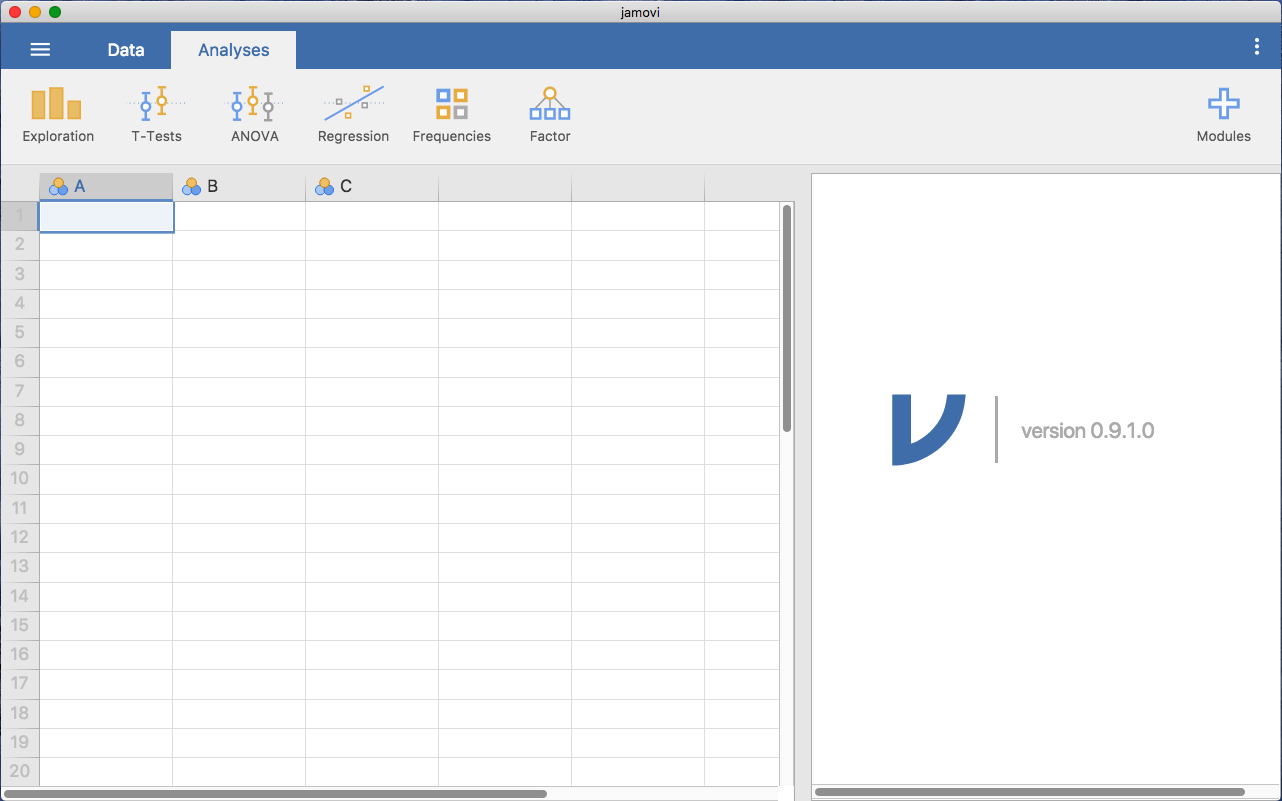
\includegraphics[width=17.81in]{img/introj/startingjamovi} 

}

\caption{jamovi looks like this when you start it}\label{fig:startingjamovi}
\end{figure}

To the left is the spreadsheet view, and to the right is where the results of statistical tests appear. Down the middle is a bar separating these two regions and this can be dragged to the left or the right to change their sizes.

It is possible to simply begin typing values into the jamovi spreadsheet as you would in any other spreadsheet software. Alternatively, existing data sets in the CSV (.csv) file format can be opened in jamovi. Additionally, you can easily import SPSS, SAS, Stata and JASP files directly into jamovi. To open a file select the File tab (three horizontal lines signify this tab) at the top left hand corner, select `Open' and then choose from the files listed on `Browse' depending on whether you want to open an example or a file stored on your computer.

\hypertarget{analyses}{%
\section{Analyses}\label{analyses}}

Analyses can be selected from the analysis ribbon or menu along the top. Selecting an analysis will present an `options panel' for that particular analysis, allowing you to assign different variables to different parts of the analysis, and select different options. At the same time, the results for the analysis will appear in the right `Results panel' and will update in real-time as you make changes to the options.

When you have the analysis set up correctly you can dismiss the analysis options by clicking the arrow to the top right of the optional panel. If you wish to return to these options, you can click on the results that were produced. In this way, you can return to any analysis that you (or say, a colleague) created earlier.

If you decide you no longer need a particular analysis, you can remove it with the results context menu. Right-clicking on the analysis results will bring up a menu and by selecting `Analysis' and then `Remove' the analysis can be removed. But more on this later. First, let's take a more detailed look at the spreadsheet view.

\hypertarget{spreadsheet}{%
\section{The spreadsheet}\label{spreadsheet}}

In jamovi data is represented in a spreadsheet with each column representing a `variable' and each row representing a `case' or `participant.'

\hypertarget{variables}{%
\subsection{Variables}\label{variables}}

The most commonly used variables in jamovi are `Data Variables,' these variables simply contain data either loaded from a data file, or `typed in' by the user. Data variables can be one of three measurement levels:

\begin{center}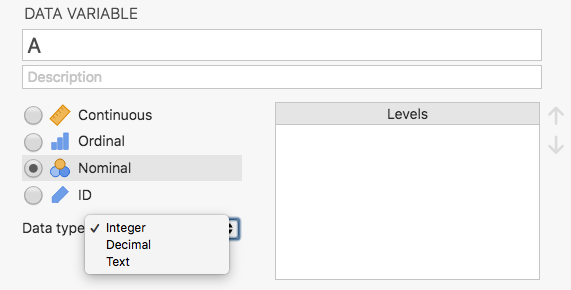
\includegraphics[width=1\linewidth]{img/introj/measurementlevels} \end{center}

These levels are designated by the symbol in the header of the variable's column.

The \emph{ID} variable type is unique to jamovi. It's intended for variables that contain identifiers that you would almost never want to analyse. For example, a persons name, or a participant ID. Specifying an ID variable type can improve performance when interacting with very large data sets.

\begin{itemize}
\tightlist
\item
  \emph{Nominal} variables are for categorical variables which are text labels, for example a column called Gender with the values Male and Female would be nominal. So would a person's name. Nominal variable values can also have a numeric value. These variables are used most often when importing data which codes values with numbers rather than text. For example, a column in a dataset may contain the values 1 for males, and 2 for females. It is possible to add nice `human-readable' labels to these values with the variable editor (more on this later).
\item
  \emph{Ordinal} variables are like Nominal variables, except the values have a specific order. An example is a Likert scale with 3 being `strongly agree' and -3 being `strongly disagree.'
\item
  \emph{Continuous} variables are variables which exist on a continuous scale. Examples might be height or weight. This is also referred to as `Interval' or `Ratio scale.'
\end{itemize}

In addition, you can also specify different data types: variables have a data type of either `Text,' `Integer' or `Decimal.'

When starting with a blank spreadsheet and typing values in the variable type will change automatically depending on the data you enter. This is a good way to get a feel for which variable types go with which sorts of data. Similarly, when opening a data file jamovi will try and guess the variable type from the data in each column. In both cases this automatic approach may not be correct, and it may be necessary to manually specify the variable type with the variable editor.

The variable editor can be opened by selecting `Setup' from the data tab or by double-clicking on the variable column header. The variable editor allows you to change the name of the variable and, for data variables, the variable type, the order of the levels, and the label displayed for each level. Changes can be applied by clicking the `tick' to the top right. The variable editor can be dismissed by clicking the `Hide' arrow.

New variables can be inserted or appended to the data set using the `add' button from the data ribbon. The `add' button also allows the addition of computed variables.

\hypertarget{computed-variables}{%
\subsection{Computed variables}\label{computed-variables}}

Computed Variables are those which take their value by performing a computation on other variables. Computed Variables can be used for a range of purposes, including log transforms, z-scores, sum-scores, negative scoring and means.

Computed variables can be added to the data set with the `add' button available on the data tab. This will produce a formula box where you can specify the formula. The usual arithmetic operators are available. Some examples of formulas are:

\texttt{A\ +\ B}

\texttt{LOG10(len)}

\texttt{MEAN(A,\ B)}

\texttt{(dose\ -\ VMEAN(dose))\ /\ VSTDEV(dose)}

In order, these are the sum of A and B, a log (base 10) transform of len, the mean of A and B, and the z-score of the variable dose. Figure \ref{fig:computedvariable} below shows the jamovi screen for the new variable computed as the z-score of dose (from the `Tooth Growth' example data set).

\begin{figure}

{\centering 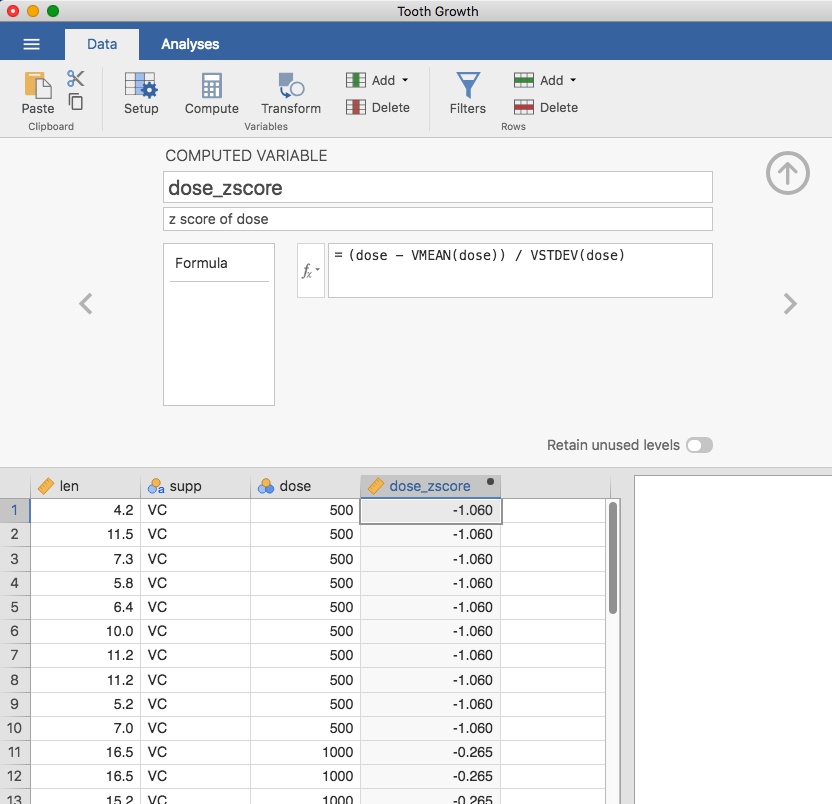
\includegraphics[width=1\linewidth]{img/introj/computedvariable} 

}

\caption{A newly computed variable, the z-score of ‘dose’}\label{fig:computedvariable}
\end{figure}

\emph{V-functions}
Several functions are already available in jamovi and available from the drop down box labelled \emph{\(f\)\textsubscript{x}}. A number of functions appear in pairs, one prefixed with a V and the other not. V functions perform their calculation on a variable as a whole, where as non-V functions perform their calculation row by row. For example, `MEAN(A, B)' will produce the mean of A and B for each row. Where as `VMEAN(A)' gives the mean of all the values in A.

\hypertarget{copypaste}{%
\subsection{Copy and Paste}\label{copypaste}}

jamovi produces nice American Psychological Association (APA) formatted tables and attractive plots. It is often useful to be able to copy and paste these, perhaps into a Word document, or into an email to a colleague. To copy results right click on the object of interest and from the menu select exactly what you want to copy. The menu allows you to choose to copy only the image or the entire analysis. Selecting ``copy'' copies the content to the clipboard and this can be pasted into other programs in the usual way. You can practice this later on when we do some analyses.

\hypertarget{syntaxmode}{%
\subsection{Syntax mode}\label{syntaxmode}}

jamovi also provides an ``R Syntax Mode.'' In this mode jamovi produces equivalent R code for each analysis. To change to syntax mode, select the Application menu to the top right of jamovi (a button with three vertical dots) and click the ``Syntax mode'' checkbox there. You can turn off syntax mode by clicking this a second time.

In syntax mode analyses continue to operate as before but now they produce R syntax, and `ascii output' like an R session. Like all results objects in jamovi, you can right click on these items (including the R syntax) and copy and paste them, for example into an R session. At present, the provided R syntax does not include the data import step and so this must be performed manually in R. There are many resources explaining how to import data into R and if you are interested we recommend you take a look at these; just search on the interweb.

\hypertarget{load}{%
\section{Loading data in jamovi}\label{load}}

There are several different types of files that are likely to be relevant to us when doing data analysis. There are two in particular that are especially important from the perspective of this book:

\begin{itemize}
\tightlist
\item
  \emph{jamovi files} are those with a \texttt{.omv} file extension. This is the standard kind of file that jamovi uses to store data, and variables and analyses.
\item
  \emph{Comma separated value (csv) files} are those with a \texttt{.csv} file extension. These are just regular old text files and they can be opened with many different software programs. It's quite typical for people to store data in csv files, precisely because they're so simple.
\end{itemize}

There are also several other kinds of data file that you might want to import into jamovi. For instance, you might want to open Microsoft Excel spreadsheets \texttt{.xls} files), or data files that have been saved in the native file formats for other statistics software, such as SPSS or SAS. Whichever file formats you are using, it's a good idea to create a folder or folders especially for your jamovi data sets and analyses and to make sure you keep these backed up regularly.

\hypertarget{importing-data-from-csv-files}{%
\subsection{Importing data from csv files}\label{importing-data-from-csv-files}}

One quite commonly used data format is the humble ``comma separated value'' file, also called a csv file, and usually bearing the file extension \texttt{.csv}. csv files are just plain old-fashioned text files and what they store is basically just a table of data. This is illustrated in Figure \ref{fig:booksalescsv}, which shows a file called \textbf{\texttt{booksales.csv}} that I've created. As you can see, each row represents the book sales data for one month. The first row doesn't contain actual data though, it has the names of the variables.

\begin{figure}

{\centering 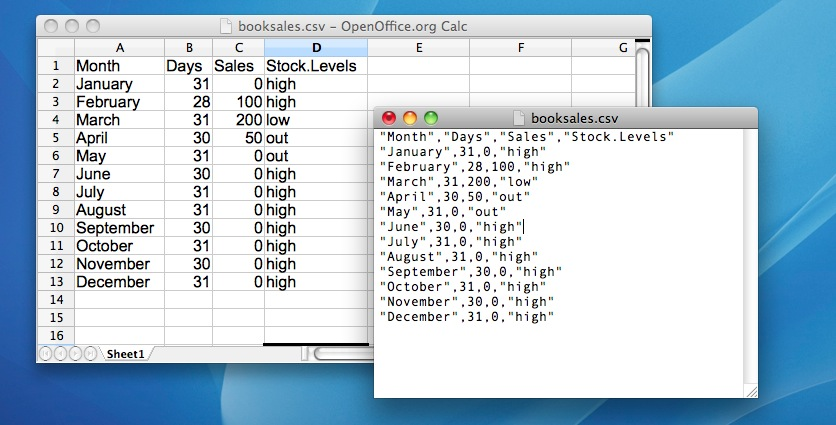
\includegraphics[width=1\linewidth]{img/mechanics/booksalescsv} 

}

\caption{The booksales.csv data file. On the left I’ve opened the file using a spreadsheet program (OpenOffice), which shows that the file is basically a table. On the right the same file is open in a standard text editor (the TextEdit program on a Mac), which shows how the file is formatted. The entries in the table are wrapped in quote marks and separated by commas.}\label{fig:booksalescsv}
\end{figure}

It's easy to open csv files in jamovi. From the top left menu (the button with three parallel lines) choose `Open' and browse to where you have stored the csv file on your computer. If you're on a Mac, it'll look like the usual Finder window that you use to choose a file; on Windows it looks like an Explorer window. An example of what it looks like on a Mac is shown in Figure \ref{fig:fileopen}. I'm assuming that you're familiar with your own computer, so you should have no problem finding the csv file that you want to import! Find the one you want, then click on the `Open' button.

\begin{figure}

{\centering 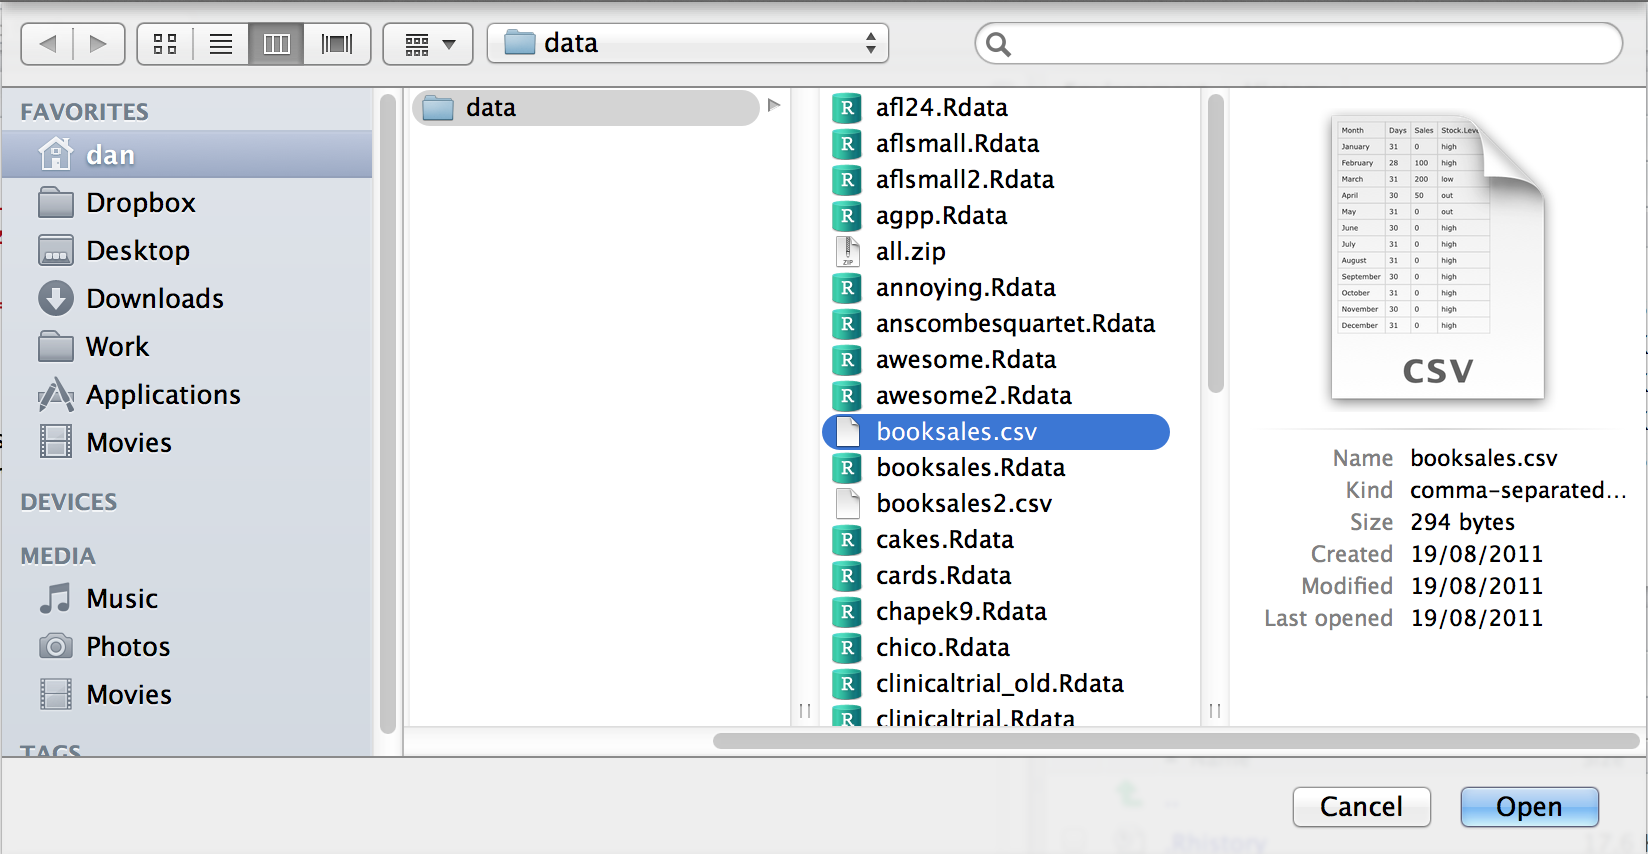
\includegraphics[width=1\linewidth]{img/mechanics/openscreen} 

}

\caption{A dialog box on a Mac asking you to select the csv file jamovi should try to import. Mac users will recognise this immediately, it’s the usual way in which a Mac asks you to find a file. Windows users won’t see this, instead they’ll see the usual explorer window that Windows always gives you when it wants you to select a file.}\label{fig:fileopen}
\end{figure}

There are a few things that you can check to make sure that the data gets imported correctly:

\begin{itemize}
\tightlist
\item
  Heading. Does the first row of the file contain the names for each variable - a ``header'' row? The \textbf{\texttt{booksales.csv}} file has a header, so that's a yes.
\item
  Separator. What character is used to separate different entries? In most csv files this will be a comma (it is ``comma separated'' after all).
\item
  Decimal. What character is used to specify the decimal point? In English speaking countries this is almost always a period (i.e., \texttt{.}). That's not universally true though, many European countries use a comma.
\item
  Quote. What character is used to denote a block of text? That's usually going to be a double quote mark ". It is for the \textbf{\texttt{booksales.csv}} file.
\end{itemize}

\hypertarget{importing}{%
\section{Importing unusual data files}\label{importing}}

Throughout this book I've assumed that your data are stored as a jamovi \texttt{.omv} file or as a ``properly''' formatted csv file. However, in real life that's not a terribly plausible assumption to make so I'd better talk about some of the other possibilities that you might run into.

\hypertarget{loading-data-from-text-files}{%
\subsection{Loading data from text files}\label{loading-data-from-text-files}}

The first thing I should point out is that if your data are saved as a text file but aren't \emph{quite} in the proper csv format then there's still a pretty good chance that jamovi will be able to open it. You just need to try it and see if it works. Sometimes though you will need to change some of the formatting. The ones that I've often found myself needing to change are:

\begin{itemize}
\tightlist
\item
  \textbf{\texttt{header}}. A lot of the time when you're storing data as a csv file the first row actually contains the column names and not data. If that's not true then it's a good idea to open up the csv file in a spreadsheet programme such as Open Office and add the header row manually.
\item
  \textbf{\texttt{sep}}. As the name ``comma separated value'' indicates, the values in a row of a csv file are usually separated by commas. This isn't universal, however. In Europe the decimal point is typically written as \texttt{,} instead of \texttt{.} and as a consequence it would be somewhat awkward to use \texttt{,} as the separator. Therefore it is not unusual to use \texttt{;} instead of \texttt{,} as the separator. At other times, I've seen a TAB character used.
\item
  \textbf{\texttt{quote}}. It's conventional in csv files to include a quoting character for textual data. As you can see by looking at the \textbf{\texttt{booksales.csv}} file, this is usually a double quote character, \texttt{"}. But sometimes there is no quoting character at all, or you might see a single quote mark \texttt{\textquotesingle{}} used instead.
\item
  \textbf{\texttt{skip}}. It's actually very common to receive CSV files in which the first few rows have nothing to do with the actual data. Instead, they provide a human readable summary of where the data came from, or maybe they include some technical info that doesn't relate to the data.
\item
  \textbf{\texttt{missing\ values}}. Often you'll get given data with missing values. For one reason or another, some entries in the table are missing. The data file needs to include a ``special'' value to indicate that the entry is missing. By default jamovi assumes that this value is \textbf{\texttt{99}}\footnote{You can change the default value for missing values in jamovi from the top right menu (three vertical dots), but this only works at the time of importing data files into jamovi. The default missing value in the dataset should not be a valid number associated with any of the variables, e.g.~you could use \textbf{\texttt{-9999}} as this is unlikely to be a valid value.}, for both numeric and text data, so you should make sure that, where necessary, all missing values in the csv file are replaced with \textbf{\texttt{99}} (or \textbf{\texttt{-9999}}; whichever you choose) before opening / importing the file into jamovi. Once you have opened / imported the file into jamovi all the missing values are converted to blank cells in the jamovi spreadsheet view.
\end{itemize}

\hypertarget{loading-data-from-spss-and-other-statistics-packages}{%
\subsection{Loading data from SPSS (and other statistics packages)}\label{loading-data-from-spss-and-other-statistics-packages}}

The commands listed above are the main ones we'll need for data files in this book. But in real life we have many more possibilities. For example, you might want to read data files in from other statistics programs. Since SPSS is probably the most widely used statistics package in psychology, it's worth mentioning that jamovi can also import SPSS data files (file extension \texttt{.sav}). Just follow the instructions above for how to open a csv file, but this time navigate to the .sav file you want to import. For SPSS files, jamovi will regard all values as missing if they are regarded as ``system missing'' files in SPSS. The `Default missings' value does not seem to work as expected when importing SPSS files, so be aware of this - you might need another step: import the SPSS file into jamovi, then export as a csv file before re-opening in jamovi.\footnote{I know this is a bit of a fudge, but it does work and hopefully this will be fixed in a later version of jamovi.}.

And that's pretty much it, at least as far as SPSS goes. As far as other statistical software goes, jamovi can also directly open / import SAS and STATA files.

\hypertarget{loading-excel-files}{%
\subsection{Loading Excel files}\label{loading-excel-files}}

A different problem is posed by Excel files. Despite years of yelling at people for sending data to me encoded in a proprietary data format, I get sent a lot of Excel files. The way to handle Excel files is to open them up first in Excel or another spreadsheet programme that can handle Excel files, and then export the data as a csv file before opening / importing the csv file into jamovi.

\hypertarget{coercion}{%
\section{Changing data from one level to another}\label{coercion}}

Sometimes you want to change the variable level. This can happen for all sorts of reasons. Sometimes when you import data from files, it can come to you in the wrong format. Numbers sometimes get imported as nominal, text values. Dates may get imported as text. ParticipantID values can sometimes be read as continuous: nominal values can sometimes be read as ordinal or even continuous. There's a good chance that sometimes you'll want to convert a variable from one measurement level into another one. Or, to use the correct term, you want to {\textbf{coerce}} the variable from one class into another.

In Section \ref{spreadsheet} we saw how to specify different variable levels, and if you want to change a variable's measurement level then you can do this in the jamovi data view for that variable. Just click the check box for the measurement level you want - continuous, ordinal, or nominal.

\hypertarget{jamovimodules}{%
\section{Installing add-on modules into jamovi}\label{jamovimodules}}

A really great feature of jamovi is the ability to install add-on modules from the jamovi library. These add-on modules have been developed by the jamovi community, i.e., jamovi users and developers who have created special software add-ons that do other, usually more advanced, analyses that go beyond the capabilities of the base jamovi program.

To install add-on modules, just click on the large ``+'' in the top right of the jamovi window, select `jamovi-library' and then browse through the various add-on modules that are available. Choose the one(s) you want, and then install them, as in Figure \ref{fig:modules}. It's that easy. The newly installed modules can then be accessed from the ``Analyses'' button bar. Try it\ldots useful add-on modules to install include ``scatr'' (added under ``Descriptives'') and ``R j.''

\begin{figure}
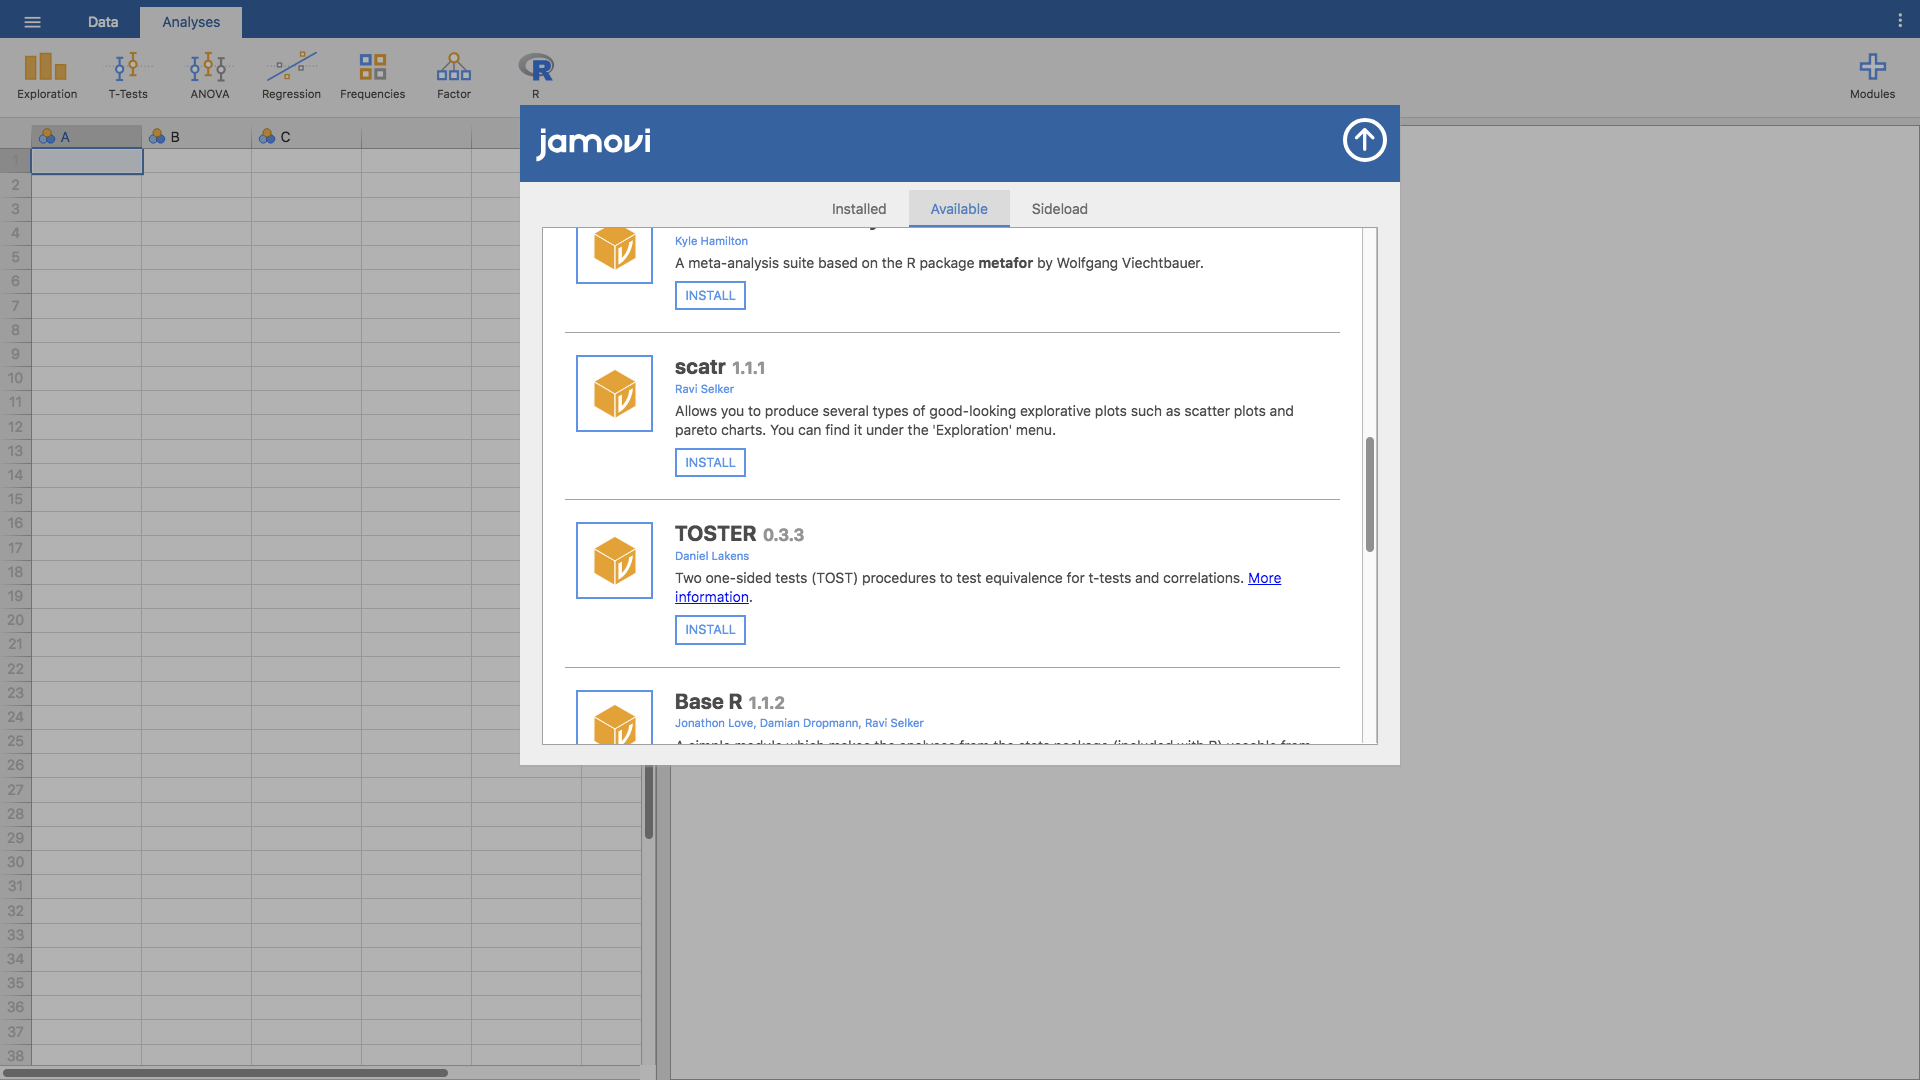
\includegraphics[width=26.67in]{img/graphics/modules} \caption{Installing add-on modules in jamovi}\label{fig:modules}
\end{figure}

\hypertarget{quittingjamovi}{%
\section{Quitting jamovi}\label{quittingjamovi}}

There's one last thing I should cover in this chapter: how to quit jamovi. It's not hard, just close the program the same way you would any other program. However, what you might want to do before you quit is save your work! There are two parts to this: saving any changes to the data set, and saving the analyses that you ran.

It is good practice to save any changes to the data set as a \emph{new} data set. That way you can always go back to the original data. To save any changes in jamovi, select ``Export''\ldots{}``Data'' from the main jamovi menu (button with three horizontal bars in the top left) and create a new file name for the changed data set.

Alternatively, you can save \emph{both} the changed data and any analyses you have undertaken by saving as a jamovi file. To do this, from the main jamovi menu select ``Save as'' and type in a file name for this ``jamovi file (.omv).'' Remember to save the file in a location where you can find it again later. I usually create a new folder for specific data sets and analyses.

\hypertarget{summary-1}{%
\section{Summary}\label{summary-1}}

\begin{itemize}
\tightlist
\item
  Section \ref{gettingjamovi}. We downloaded and installed jamovi, and started it up.
\item
  Section \ref{analyses}. We very briefly oriented to the part of jamovi where analyses are done and results appear, but then deferred this until later in the book.
\item
  Section \ref{spreadsheet}. We spent more time looking at the spreadsheet part of jamovi, and considered different variable types, and how to compute new variables.
\item
  Section \ref{load}. We also saw how to load data files in jamovi.
\item
  Section \ref{importing}. Then we figured out how to open other data files, from different file types.
\item
  Section \ref{coercion}. And saw that sometimes we need to coerce data from one type to another.
\item
  Section \ref{jamovimodules}. Installing add-on modules from the jamovi community really extends jamovi capabilities.
\item
  Section \ref{quittingjamovi}. Finally, we looked at good practice in terms of saving your data set and analyses when you have finished and are about to quit jamovi.
\end{itemize}

\hypertarget{part-iii.-working-with-data}{%
\chapter*{Part III. Working with data}\label{part-iii.-working-with-data}}
\addcontentsline{toc}{chapter}{Part III. Working with data}

\hypertarget{graphics}{%
\chapter{Drawing graphs}\label{graphics}}

~~~~~\emph{Above all else show the data.}\\
\hspace*{0.333em}\hspace*{0.333em}\hspace*{0.333em}\hspace*{0.333em}\hspace*{0.333em}\hspace*{0.333em}\hspace*{0.333em}\hspace*{0.333em}\hspace*{0.333em}\hspace*{0.333em}\hspace*{0.333em}\hspace*{0.333em}\hspace*{0.333em}\hspace*{0.333em}\hspace*{0.333em}\hspace*{0.333em}\hspace*{0.333em}-- Edward Tufte\footnote{The origin of this quote is Tufte's lovely book\emph{The Visual Display of Quantitative Information}}

Visualising data is one of the most important tasks facing the data analyst. It's important for two distinct but closely related reasons. Firstly, there's the matter of drawing `presentation graphics,' displaying your data in a clean, visually appealing fashion makes it easier for your reader to understand what you're trying to tell them. Equally important, perhaps even more important, is the fact that drawing graphs helps \emph{you} to understand the data. To that end, it's important to draw `exploratory graphics' that help you learn about the data as you go about analysing it. These points might seem pretty obvious but I cannot count the number of times I've seen people forget them.

To give a sense of the importance of this chapter, I want to start with a classic illustration of just how powerful a good graph can be. To that end, Figure \ref{fig:snowmap1} shows a redrawing of one of the most famous data visualisations of all time. This is John Snow's 1854 map of cholera deaths. The map is elegant in its simplicity. In the background we have a street map which helps orient the viewer. Over the top we see a large number of small dots, each one representing the location of a cholera case. The larger symbols show the location of water pumps, labelled by name. Even the most casual inspection of the graph makes it very clear that the source of the outbreak is almost certainly the Broad Street pump. Upon viewing this graph Dr Snow arranged to have the handle removed from the pump and ended the outbreak that had killed over 500 people. Such is the power of a good data visualisation.

\begin{figure}
\centering
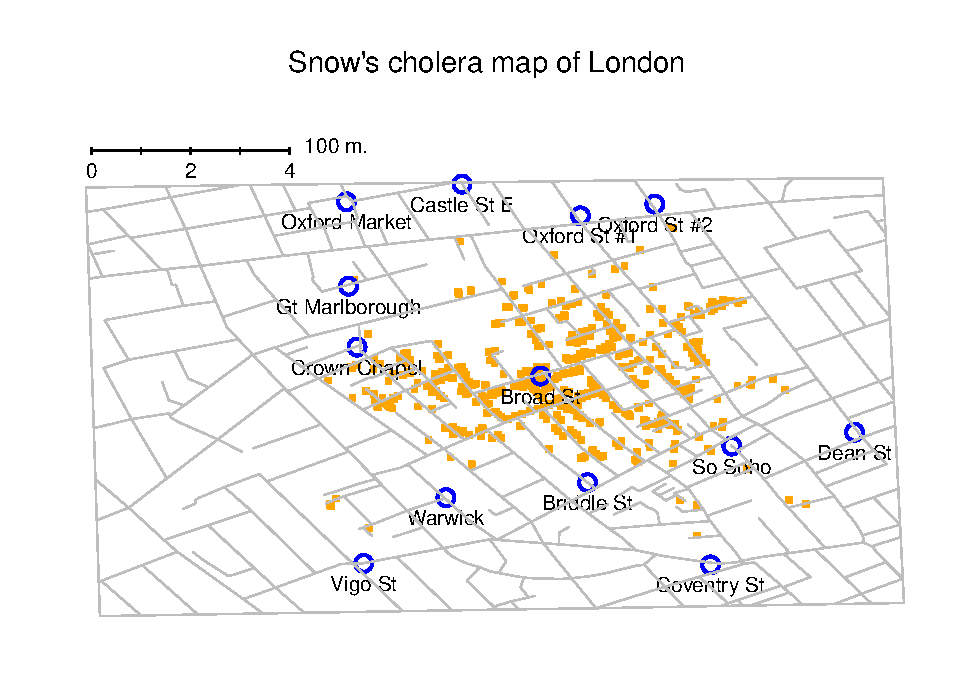
\includegraphics{lsj_files/figure-latex/snowmap1-1.pdf}
\caption{\label{fig:snowmap1}A stylised redrawing of John Snow's original cholera map. Each small dot represents the location of a cholera case and each large circle shows the location of a well. As the plot makes clear, the cholera outbreak is centred very closely on the Broad St pump}
\end{figure}

The goals in this chapter are twofold. First, to discuss several fairly standard graphs that we use a lot when analysing and presenting data, and second to show you how to create these graphs in jamovi. The graphs themselves tend to be pretty straightforward, so in one respect this chapter is pretty simple. Where people usually struggle is learning how to produce graphs, and especially learning how to produce good graphs. Fortunately, learning how to draw graphs in jamovi is reasonably simple as long as you're not too picky about what your graph looks like. What I mean when I say this is that jamovi has a lot of \emph{very} good default graphs, or plots, that most of the time produce a clean, high-quality graphic. However, on those occasions when you do want to do something non-standard, or if you need to make highly specific changes to the figure, then the graphics functionality in jamovi is not yet capable of supporting advanced work or detail editing.

\hypertarget{hist}{%
\section{Histograms}\label{hist}}

Let's begin with the humble {\textbf{histogram}}. Histograms are one of the simplest and most useful ways of visualising data. They make most sense when you have an interval or ratio scale variable (e.g., the \textbf{\texttt{afl.margins}} data from Chapter \ref{descriptives}) and what you want to do is get an overall impression of the variable. Most of you probably know how histograms work, since they're so widely used, but for the sake of completeness I'll describe them. All you do is divide up the possible values into {\textbf{bins}} and then count the number of observations that fall within each bin. This count is referred to as the frequency or density of the bin and is displayed as a vertical bar. Ihe AFL winning margins data there are 33 games in which the winning margin was less than 10 points and it is this fact that is represented by the height of the leftmost bar that we showed earlier in Chapter \ref{descriptives}, Figure \ref{fig:histogram1}. With these earlier graphs we used an advanced plotting package in R which, for now, is beyond the capability of jamovi. But jamovi gets us close, and drawing this histogram in jamovi is pretty straightforward. Open up the `plots' options under `Exploration' - `Descriptives' and click the `histogram' check box, as in Figure \ref{fig:jamovihistogram}. jamovi defaults to labelling the y-axis as `density' and the x-axis with the variable name. The {\textbf{bins}} are selected automatically, and there is no scale, or count, information on the y-axis unlike the previous Figure \ref{fig:histogram1}. But this does not matter too much because after all what we are really interested in is our impression of the shape of the distribution: is it normally distributed or is there a skew or kurtosis? Our first impressions of these characteristics come from drawing a {\textbf{histogram}}.

\begin{figure}

{\centering 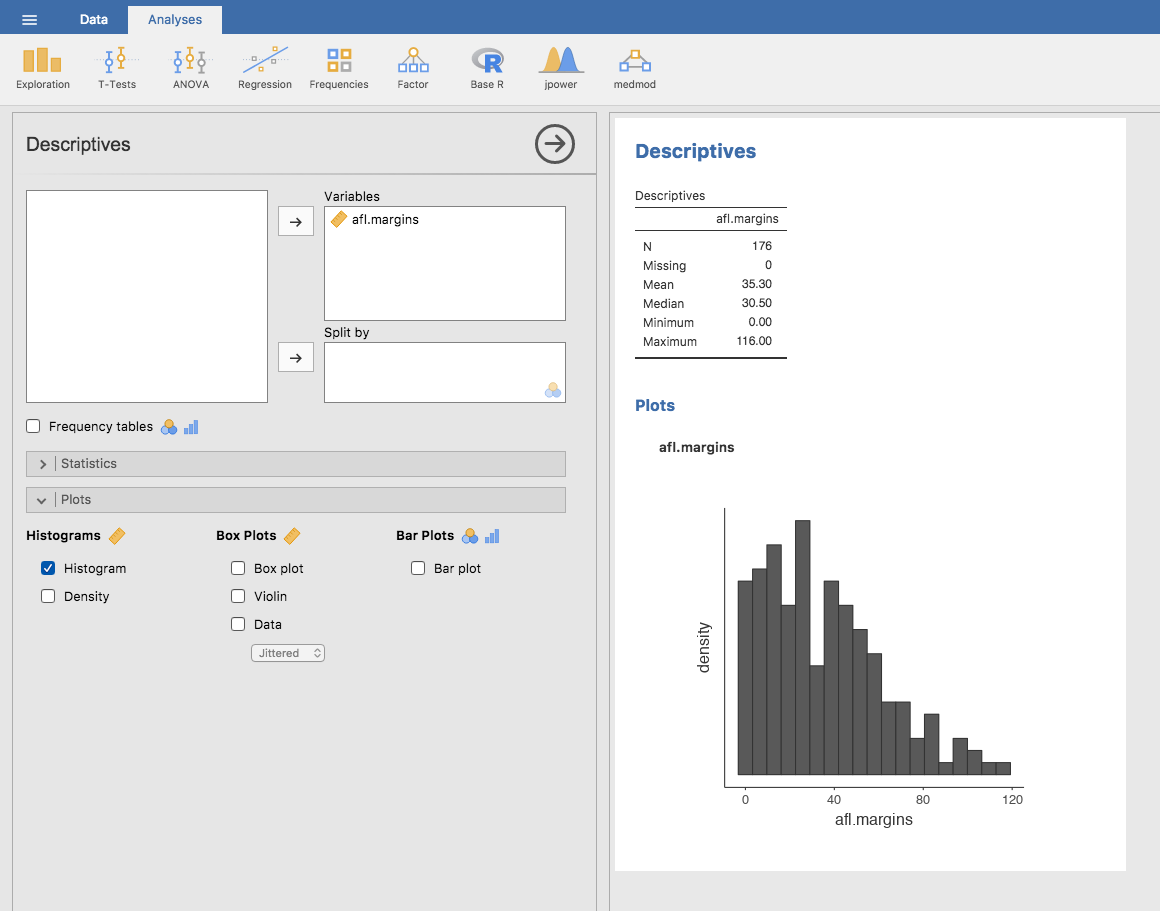
\includegraphics[width=1\linewidth]{img/graphics/jamovi_histogram} 

}

\caption{jamovi screen showing the histogram check box}\label{fig:jamovihistogram}
\end{figure}

One additional feature that jamovi provides is the ability to plot a `Density' curve. You can do this by clicking the `Density' check box under the `Plots' options (and unchecking `Histogram'), and this gives us the plot shown in Figure \ref{fig:histogram2}. A density plot visualises the distribution of data over a continuous interval or time period. This chart is a variation of a histogram that uses {\textbf{kernel smoothing}} to plot values, allowing for smoother distributions by smoothing out the noise. The peaks of a density plot help display where values are concentrated over the interval. An advantage density plots have over histograms is that they are better at determining the distribution shape because they're not affected by the number of bins used (each bar used in a typical histogram). A histogram comprising of only 4 bins wouldn't produce a distinguishable enough shape of distribution as a 20-bin histogram would. However, with density plots, this isn't an issue.

\begin{figure}

{\centering 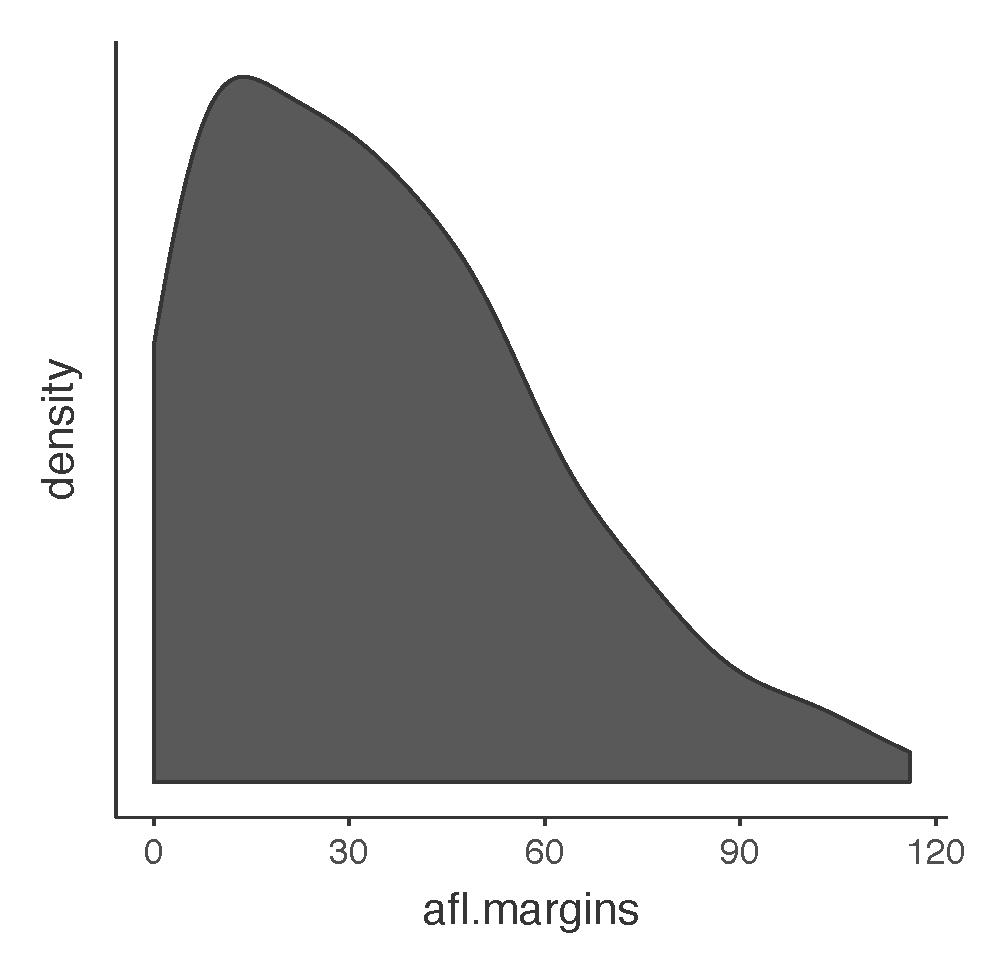
\includegraphics[width=1\linewidth]{img/graphics/histogram2} 

}

\caption{A density plot of the **`afl.margins`** variable plotted in jamovi}\label{fig:histogram2}
\end{figure}

Although this image would need a lot of cleaning up in order to make a good presentation graphic (i.e., one you'd include in a report), it nevertheless does a pretty good job of describing the data. In fact, the big strength of a histogram or density plot is that (properly used) it does show the entire spread of the data, so you can get a pretty good sense about what it looks like. The downside to histograms is that they aren't very compact. Unlike some of the other plots I'll talk about it's hard to cram 20-30 histograms into a single image without overwhelming the viewer. And of course, if your data are nominal scale then histograms are useless.

\hypertarget{boxplots}{%
\section{Boxplots}\label{boxplots}}

Another alternative to histograms is a {\textbf{boxplot}}, sometimes called a `box and whiskers' plot. Like histograms they're most suited to interval or ratio scale data. The idea behind a boxplot is to provide a simple visual depiction of the median, the interquartile range, and the range of the data. And because they do so in a fairly compact way boxplots have become a very popular statistical graphic, especially during the exploratory stage of data analysis when you're trying to understand the data yourself. Let's have a look at how they work, again using the \textbf{\texttt{afl.margins}} data as our example.

\begin{figure}

{\centering 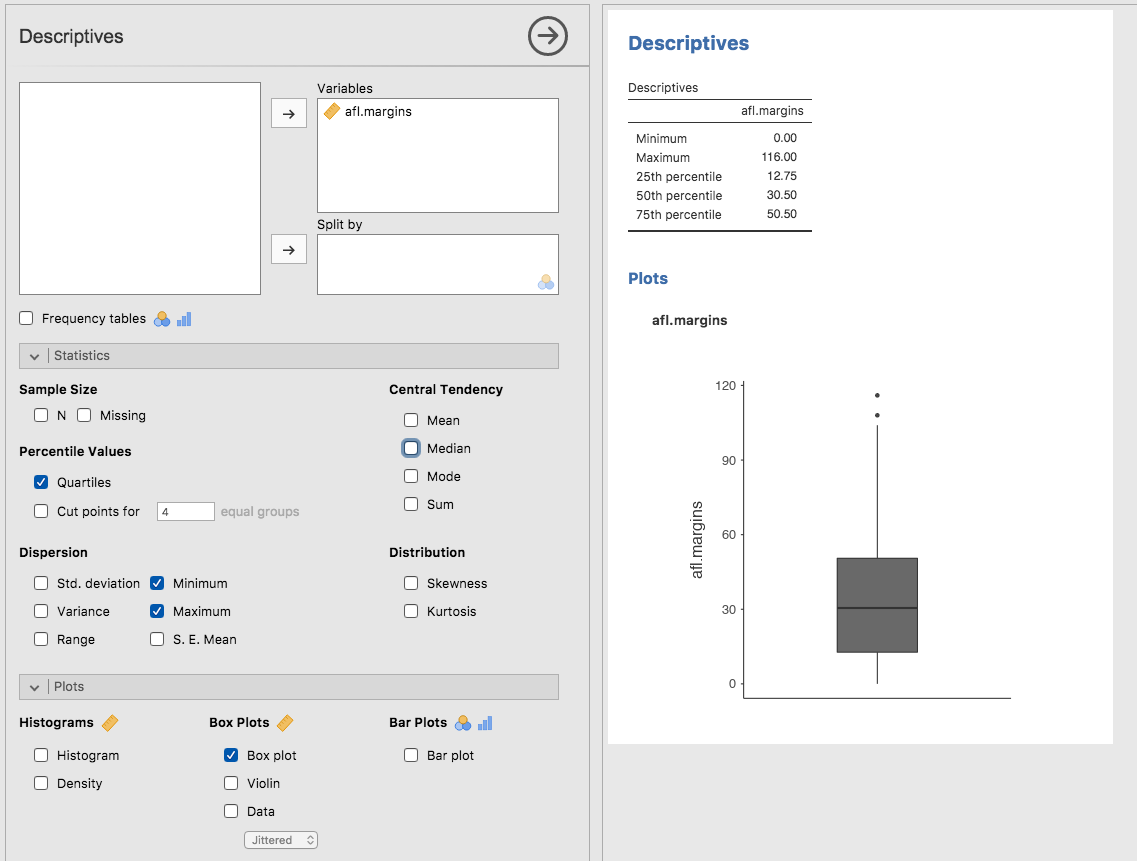
\includegraphics[width=1\linewidth]{img/graphics/boxplot1} 

}

\caption{A box plot of the **`afl.margins`** variable plotted in jamovi}\label{fig:boxplot1}
\end{figure}

The easiest way to describe what a boxplot looks like is just to draw one. Click on the `Box plot' check box and you will get the plot shown on the lower right of Figure \ref{fig:boxplot1}. jamovi has drawn the most basic boxplot possible. When you look at this plot this is how you should interpret it: the thick line in the middle of the box is the median; the box itself spans the range from the 25th percentile to the 75th percentile; and the `whiskers' go out to the most extreme data point that doesn't exceed a certain bound. By default, this value is 1.5 times the interquartile range (IQR), calculated as \texttt{25th\ percentile\ -\ (1.5*IQR)} for the lower boundary, and \texttt{75th\ percentile\ +\ (1.5*IQR)} for the upper boundary. Any observation whose value falls outside this range is plotted as a circle or dot instead of being covered by the whiskers, and is commonly referred to as an {\textbf{outlier}}. For our AFL margins data there are two observations that fall outside this range, and these observations are plotted as dots (the upper boundary is 107, and looking over the data column in the spreadsheet there are two observations with values higher than this, 108 and 116, so these are the dots).

\hypertarget{violinplots}{%
\subsection{Violin plots}\label{violinplots}}

\begin{figure}

{\centering 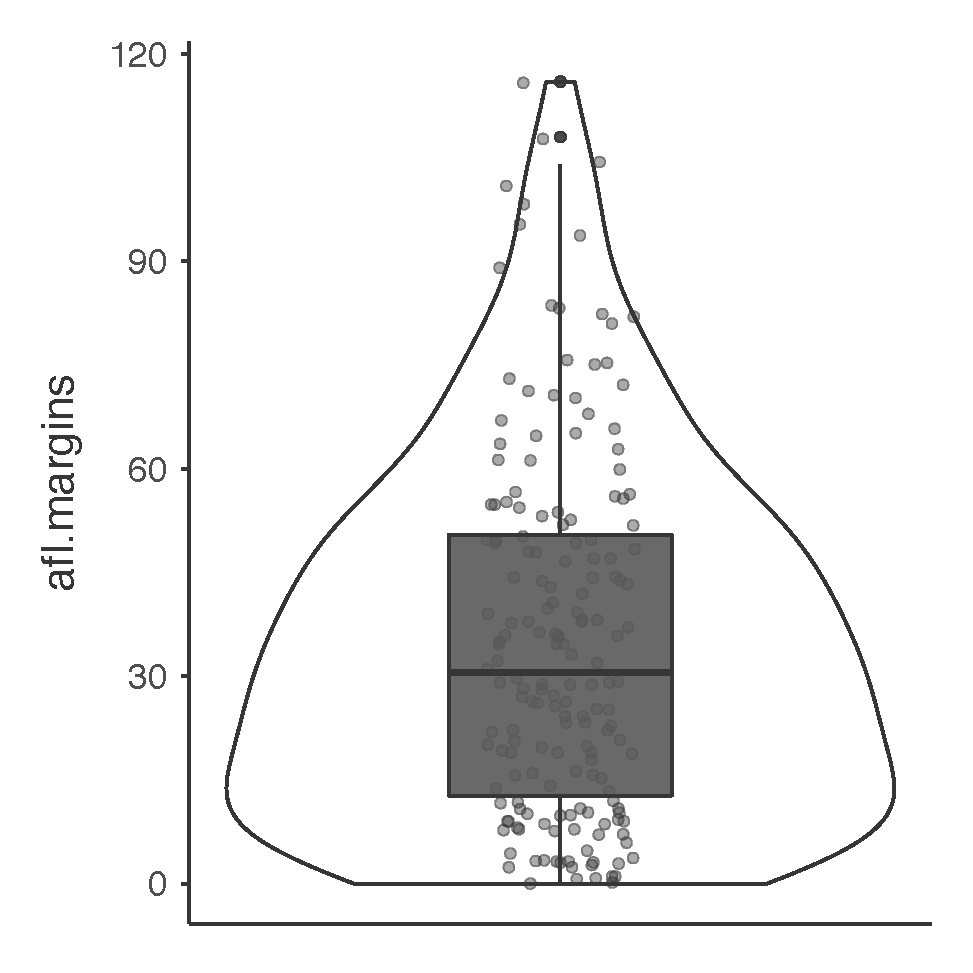
\includegraphics[width=1\linewidth]{img/graphics/boxplot2} 

}

\caption{A violin plot of the **`afl.margins`** variable plotted in jamovi, also showing a box plot and data points}\label{fig:boxplot2}
\end{figure}

A variation to the traditional box plot is the violin plot. Violin plots are similar to box plots except that they also show the kernel probability density of the data at different values. Typically, violin plots will include a marker for the median of the data and a box indicating the interquartile range, as in standard box plots. In jamovi you can achieve this sort of functionality by checking both the `Violin' and the `Box plot' check boxes. See Figure \ref{fig:boxplot2}, which also has the `Data' check box turned on to show the actual data points on the plot. This does tend to make the graph a bit too busy though, in my opinion. Clarity is simplicity, so in practice it might be better to just use a simple box plot.

\hypertarget{multipleboxplots}{%
\subsection{Drawing multiple boxplots}\label{multipleboxplots}}

One last thing. What if you want to draw multiple boxplots at once? Suppose, for instance, I wanted separate boxplots showing the AFL margins not just for 2010 but for every year between 1987 and 2010. To do that the first thing we'll have to do is find the data. These are stored in the \textbf{\texttt{aflsmall2.csv}} file. So let's load it into jamovi and see what is in it. You will see that it is a pretty big data set. It contains 4296 games and the variables that we're interested in. What we want to do is have jamovi draw boxplots for the \textbf{\texttt{margin}} variable, but plotted separately for each \textbf{\texttt{year}}. The way to do this is to move the \texttt{year} variable across into the `Split by' box, as in Figure \ref{fig:splitfile1}

\begin{figure}

{\centering 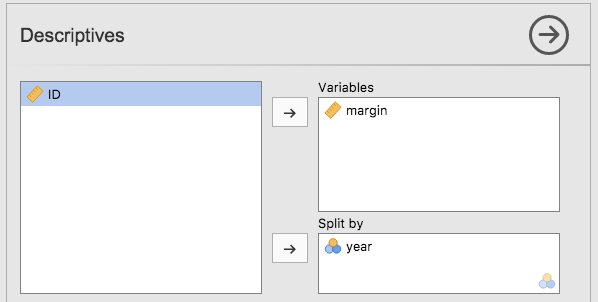
\includegraphics[width=1\linewidth]{img/graphics/splitfile1} 

}

\caption{jamovi screen shot showing the 'Split by' window}\label{fig:splitfile1}
\end{figure}

The result is shown in Figure \ref{fig:boxplot3}. This version of the box plot, split by year, gives a sense of why it's sometimes useful to choose box plots instead of histograms. It's possible to get a good sense of what the data look like from year to year without getting overwhelmed with too much detail. Now imagine what would have happened if I'd tried to cram 24 histograms into this space: no chance at all that the reader is going to learn anything useful.

\begin{figure}

{\centering 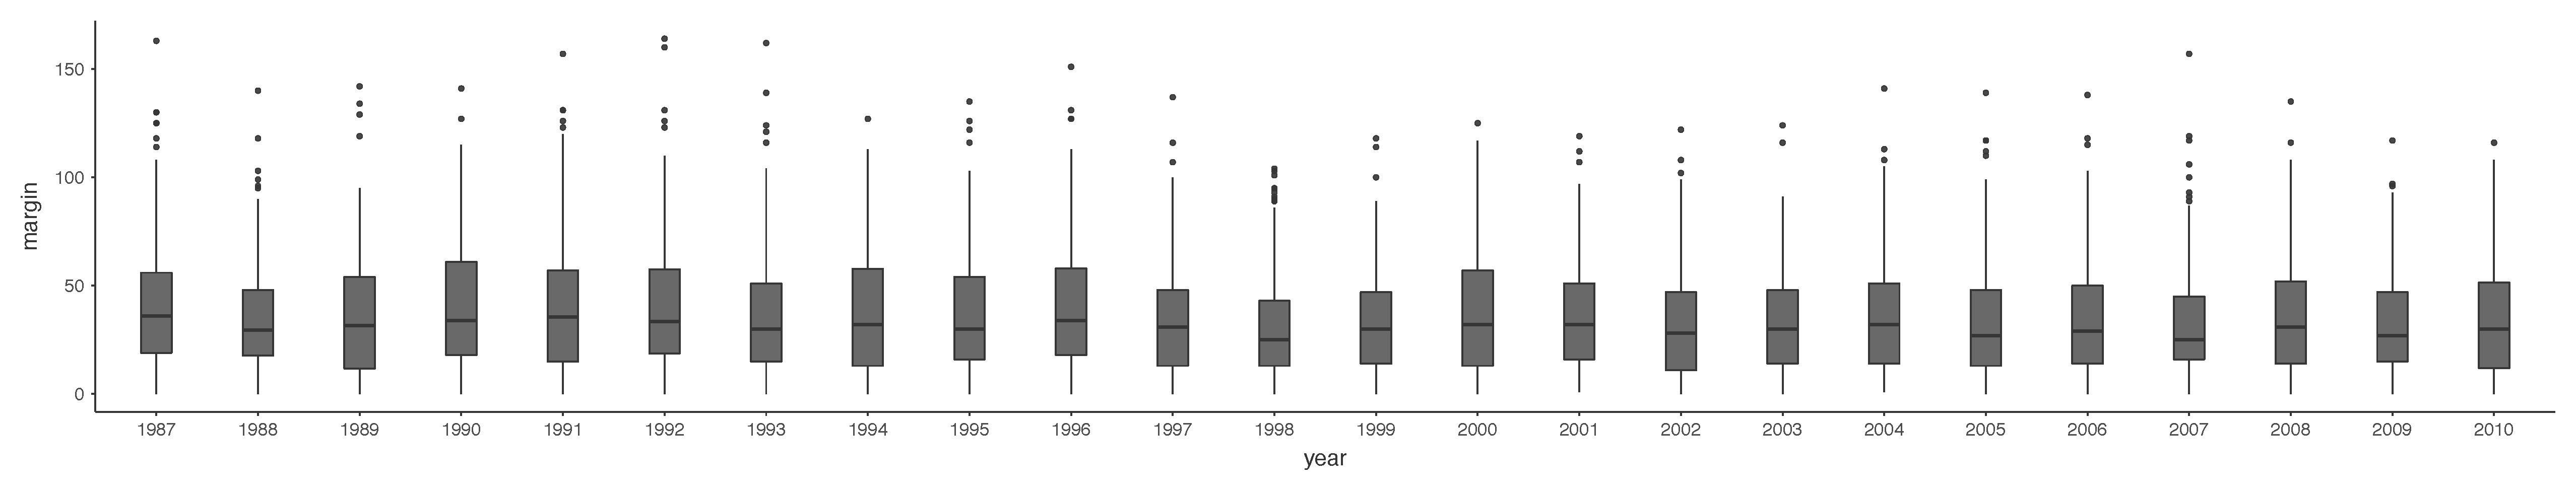
\includegraphics[width=1\linewidth]{img/graphics/boxplot3} 

}

\caption{Multiple boxplots plotted in jamovi, for the **`margin`** by **`year`** variables in the **`aflsmall2`** data set}\label{fig:boxplot3}
\end{figure}

\hypertarget{boxplotoutliers}{%
\subsection{Using box plots to detect outliers}\label{boxplotoutliers}}

Because the boxplot automatically separates out those observations that lie outside a certain range, depicting them with a dot in jamovi, people often use them as an informal method for detecting {\textbf{outliers}}: observations that are `suspiciously' distant from the rest of the data. Here's an example. Suppose that I'd drawn the boxplot for the AFL margins data and it came up looking like Figure \ref{fig:boxplot4}. It's pretty clear that something funny is going on with two of the observations. Apparently, there were two games in which the margin was over 300 points! That doesn't sound right to me. Now that I've become suspicious it's time to look a bit more closely at the data. In jamovi you can quickly find out which of these observations are suspicious and then you can go back to the raw data to see if there has been a mistake in data entry. To do this you need to set up a filter so that only those observations with values over a certain threshold are included. In our example, the threshold is over 300, so that is the filter we will create. First, click on the `Filters' button at the top of the jamovi window, and then type `margin \(>\) 300' into the filter field, as in Figure \ref{fig:filter1}.

\begin{figure}

{\centering 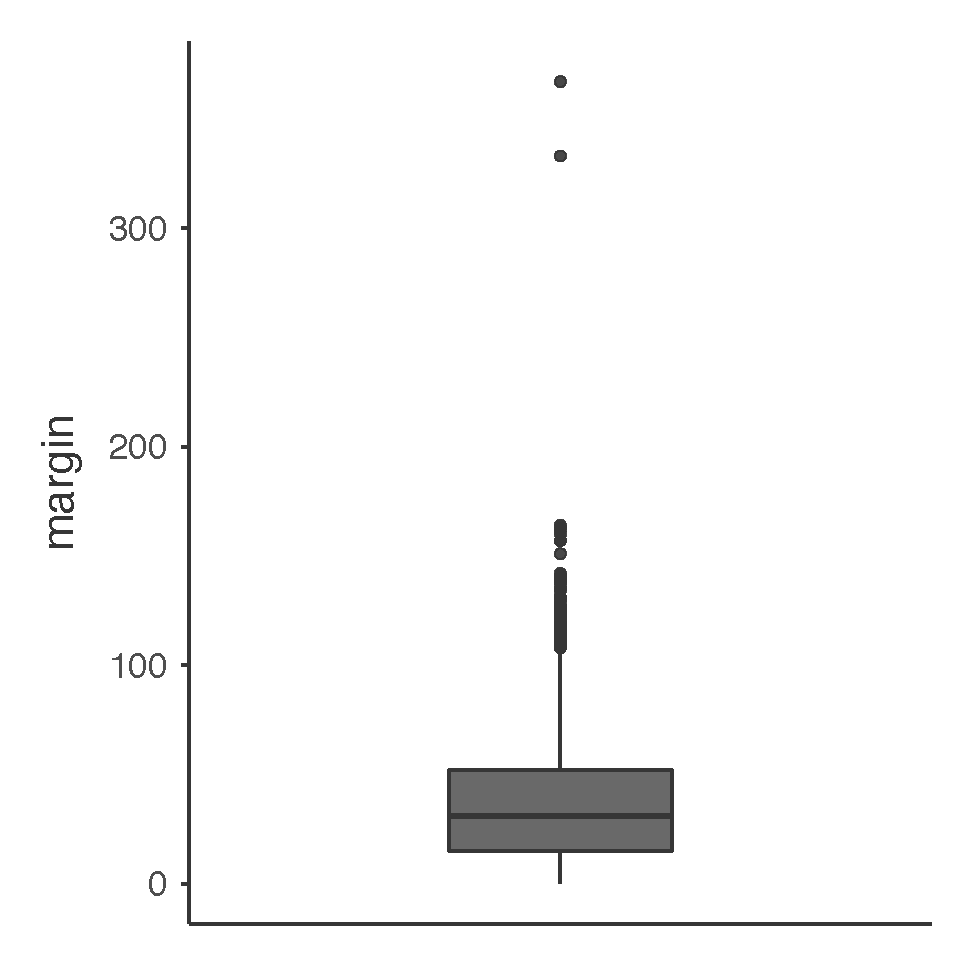
\includegraphics[width=1\linewidth]{img/graphics/boxplot4} 

}

\caption{A boxplot showing two very suspicious outliers!}\label{fig:boxplot4}
\end{figure}

\begin{figure}

{\centering 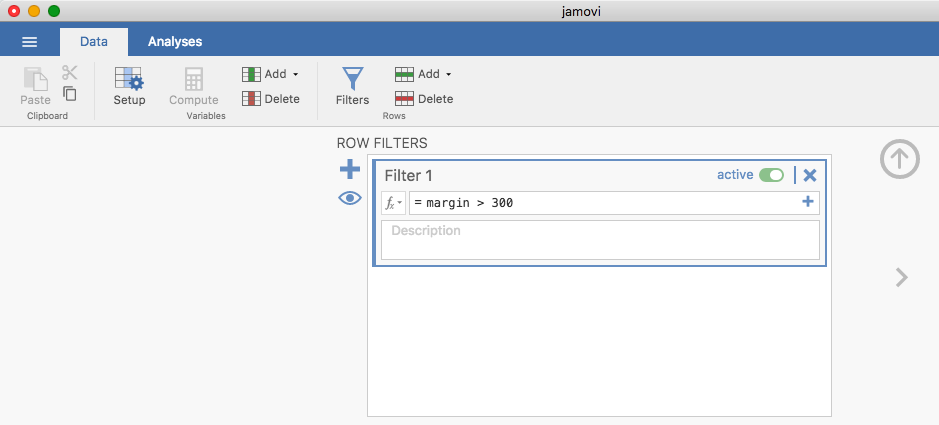
\includegraphics[width=1\linewidth]{img/graphics/filter1} 

}

\caption{the jamovi filter screen}\label{fig:filter1}
\end{figure}

This filter creates a new column in the spreadsheet view where only those observations that pass the filter are included. One neat way to quickly identify which observations these are is to tell jamovi to produce a `Frequency table' (in the `Exploration' - `Descriptives' window) for the ID variable (which must be a nominal variable otherwise the Frequency table is not produced). In Figure \ref{fig:filter2} you can see that the ID values for the observations where the margin was over 300 are \texttt{14} and \texttt{134}. These are suspicious cases, or observations, where you should go back to the original data source to find out what is going on.

\begin{figure}

{\centering 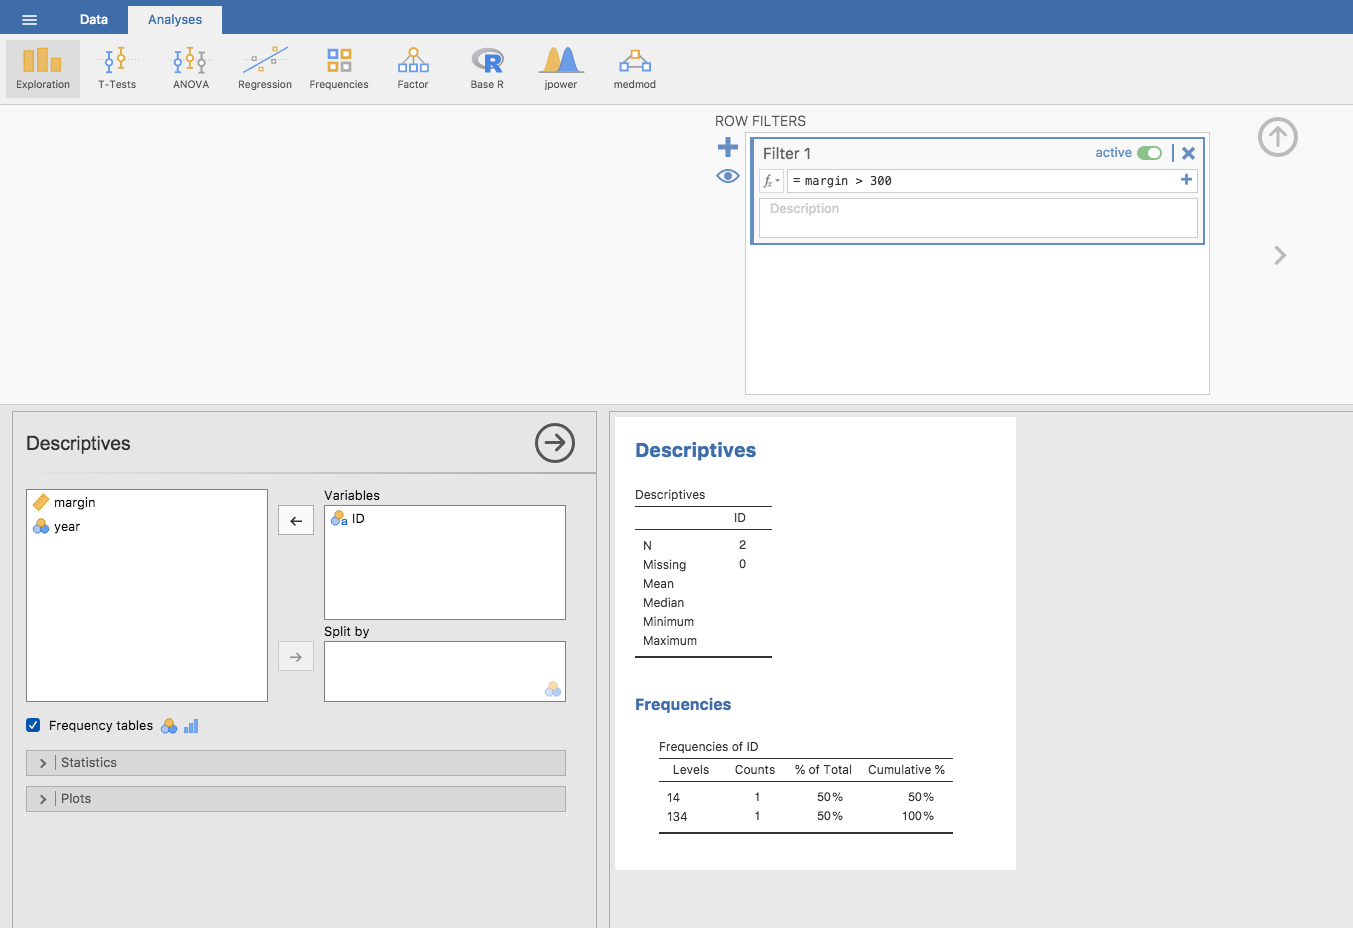
\includegraphics[width=1\linewidth]{img/graphics/filter2} 

}

\caption{Frequency table for `ID` showing the ID numbers for the two suspicious outliers: `14` and `134`}\label{fig:filter2}
\end{figure}

Usually you find that someone has just typed in the wrong number. Whilst this might seem like a silly example, I should stress that this kind of thing actually happens a lot. Real world data sets are often riddled with stupid errors, especially when someone had to type something into a computer at some point. In fact, there's actually a name for this phase of data analysis and in practice it can take up a huge chunk of our time: {\textbf{data cleaning}}. It involves searching for typing mistakes (`typos'), missing data and all sorts of other obnoxious errors in raw data files.

For less extreme values, even if they are flagged in a a boxplot as outliers, the decision about whether to include outliers or exclude them in any analysis depends heavily on \emph{why} you think the data look they way they do and what you want to use the data \emph{for}. You really need to exercise good judgement here. If the outlier looks legitimate to you, then keep it. In any case, I'll return to the topic again in Section \ref{regressiondiagnostics}.

\hypertarget{bargraph}{%
\section{Bar graphs}\label{bargraph}}

Another form of graph that you often want to plot is the {\textbf{bar graph}}. Let's use the \textbf{\texttt{afl.finalists}} data set with the \textbf{\texttt{afl.finalists}} variable that I introduced in Section \ref{mode}. What I want to do is draw a bar graph that displays the number of finals that each team has played in over the time spanned by the \textbf{\texttt{afl.finalists}} data set. There are lots of teams, but I am particularly interested in just four: Brisbane, Carlton, Fremantle and Richmond. So the first step is to set up a filter so just those four teams are included in the bar graph. This is straightforward in jamovi and you can do it by using the `Filters' function that we used previously. Open up the `Filters' screen and type in the following:

\texttt{afl.finalists\ ==\ ‘Brisbane’\ or\ afl.finalists\ ==\ ‘Carlton’\ or\ afl.finalists\ ==\ ‘Fremantle’\ or\ afl.finalists\ ==\ ‘Richmond’}\footnote{jamovi uses the symbol \texttt{==} here to mean `matches.'}

When you have done this you will see, in the `Data' view, that jamovi has filtered out all values apart from those we have specified. Next, open up the `Exploration' - `Descriptives' window and click on the `Bar plot' check box (remember to move the \textbf{\texttt{afl.finalists}} variable across into the `Variables' box so that jamovi knows which variable to use). You should then get a bar graph, something like that shown in Figure \ref{fig:bar1}.

\begin{figure}

{\centering 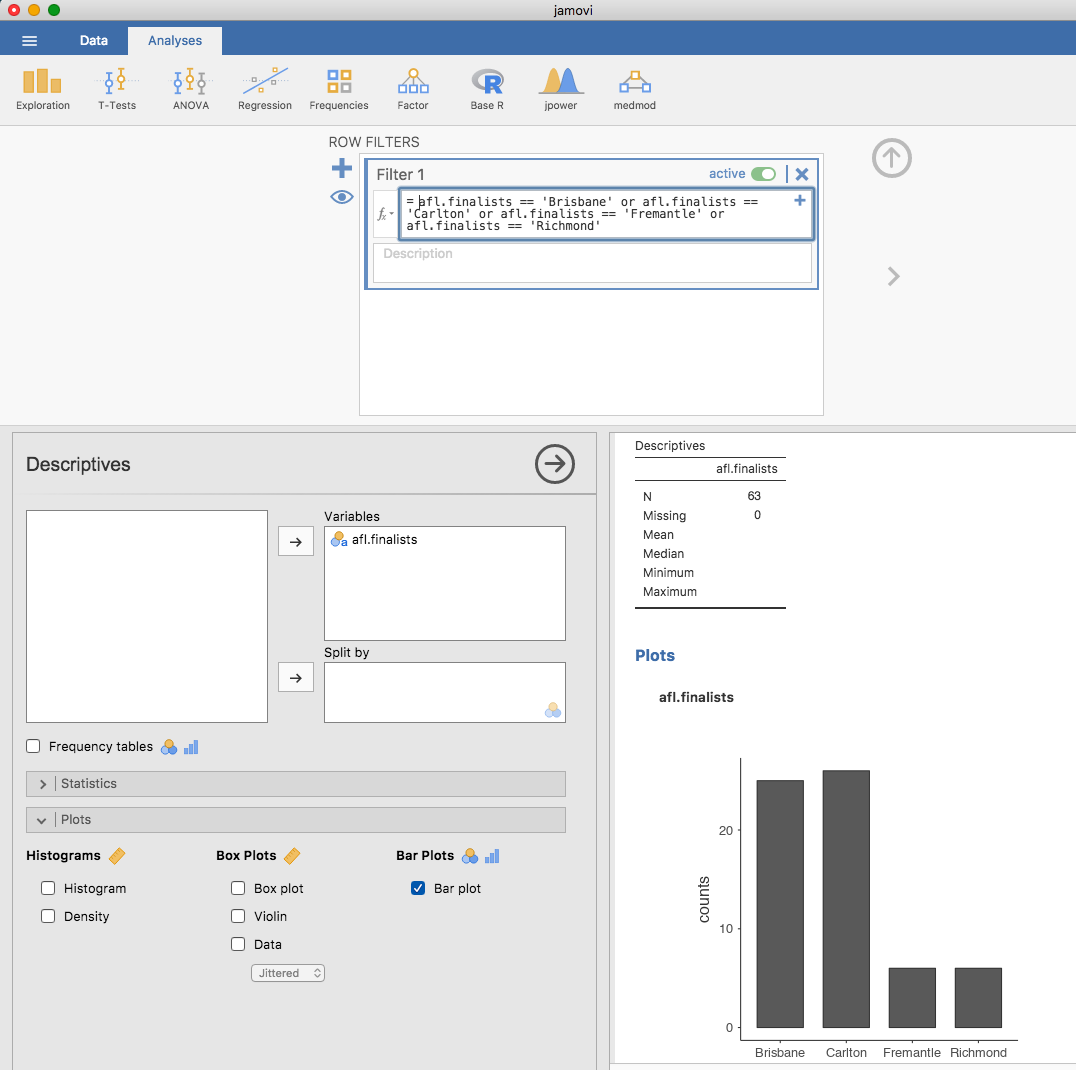
\includegraphics[width=1\linewidth]{img/graphics/bar1} 

}

\caption{Filtering to include just four AFL teams, and drawing a bar plot in jamovi}\label{fig:bar1}
\end{figure}

\hypertarget{saveimage}{%
\section{Saving image files using jamovi}\label{saveimage}}

Hold on, you might be thinking. What's the good of being able to draw pretty pictures in jamovi if I can't save them and send them to friends to brag about how awesome my data is? How do I save the picture? Simple. Just right click on the plot image and save it to a file, either as `eps,' `svg' or `pdf.' These formats all produce nice images that you can the send to your friends, or include in your assignments or papers.

\hypertarget{summary-2}{%
\section{Summary}\label{summary-2}}

Perhaps I'm a simple minded person, but I love pictures. Every time I write a new scientific paper one of the first things I do is sit down and think about what the pictures will be. In my head an article is really just a sequence of pictures linked together by a story. All the rest of it is just window dressing. What I'm really trying to say here is that the human visual system is a very powerful data analysis tool. Give it the right kind of information and it will supply a human reader with a massive amount of knowledge very quickly. Not for nothing do we have the saying `a picture is worth a thousand words.' With that in mind, I think that this is one of the most important chapters in the book. The topics covered were:

\begin{itemize}
\tightlist
\item
  \emph{Common plots}. Much of the chapter was focused on standard graphs that statisticians like to produce: histograms (Section \ref{hist}), boxplots (Section \ref{boxplots}) and bar graphs (Section \ref{bargraph})
\item
  \emph{Saving image files}. Importantly, we also covered how to export your pictures (Section \ref{saveimage})
\end{itemize}

One final thing to point out. Whilst jamovi produces some really neat default graphics, editing the plots is currently not possible. For more advanced graphics and plotting capability the packages available in R are much more powerful. One of the most popular graphics systems is provided by the \texttt{ggplot2} package (see \url{http://ggplot2.org/}), which is loosely based on `The grammar of graphics' (\protect\hyperlink{ref-Wilkinson2006}{Wilkinson et al., 2006}). It's not for novices. You need to have a pretty good grasp of R before you can start using it, and even then it takes a while to really get the hang of it. But when you're ready it's worth taking the time to teach yourself, because it's a much more powerful and cleaner system.

\hypertarget{datahandling}{%
\chapter{Pragmatic matters}\label{datahandling}}

~~~~~~\emph{The garden of life never seems to confine itself to the plots philosophers have laid out for its convenience. Maybe a few more tractors would do the trick.}\\
\hspace*{0.333em}\hspace*{0.333em}\hspace*{0.333em}\hspace*{0.333em}\hspace*{0.333em}\hspace*{0.333em}\hspace*{0.333em}\hspace*{0.333em}\hspace*{0.333em}\hspace*{0.333em}\hspace*{0.333em}\hspace*{0.333em}\hspace*{0.333em}\hspace*{0.333em}\hspace*{0.333em}\hspace*{0.333em}\hspace*{0.333em}\hspace*{0.333em}\hspace*{0.333em}\hspace*{0.333em}\hspace*{0.333em}\hspace*{0.333em}\hspace*{0.333em}\hspace*{0.333em}\hspace*{0.333em}\hspace*{0.333em}\hspace*{0.333em}\hspace*{0.333em}\hspace*{0.333em}\hspace*{0.333em}-- Roger Zelazny\footnote{The quote comes from \emph{Home is the Hangman}, published in 1975.}

This is a somewhat strange chapter, even by my standards. My goal in this chapter is to talk a bit more honestly about the realities of working with data than you'll see anywhere else in the book. The problem with real world data sets is that they are \emph{messy}. Very often the data file that you start out with doesn't have the variables stored in the right format for the analysis you want to do. Sometimes there might be a lot of missing values in your data set. Sometimes you only want to analyse a subset of the data. Et cetera. In other words, there's a lot of {\textbf{data manipulation}} that you need to do just to get the variables in your data set into the format that you need it. The purpose of this chapter is to provide a basic introduction to these pragmatic topics. Although the chapter is motivated by the kinds of practical issues that arise when manipulating real data, I'll stick with the practice that I've adopted through most of the book and rely on very small, toy data sets that illustrate the underlying issue. Because this chapter is essentially a collection of techniques and doesn't tell a single coherent story, it may be useful to start with a list of topics:

\begin{itemize}
\tightlist
\item
  Section \ref{freqtables}. Tabulating data.
\item
  Section \ref{logicals}. Using logical expressions.
\item
  Section \ref{transform}. Transforming or recoding a variable.
\item
  Section \ref{mathfunc}. Some useful mathematical functions.
\item
  Section \ref{subset}. Extracting a subset of a data set.
\end{itemize}

As you can see, the list of topics that the chapter covers is pretty broad, and there's a \emph{lot} of content there. Even though this is one of the longest and hardest chapters in the book, I'm really only scratching the surface of several fairly different and important topics. My advice, as usual, is to read through the chapter once and try to follow as much of it as you can. Don't worry too much if you can't grasp it all at once, especially the later sections. The rest of the book is only lightly reliant on this chapter so you can get away with just understanding the basics. However, what you'll probably find is that later on you'll need to flick back to this chapter in order to understand some of the concepts that I refer to here.

\hypertarget{freqtables}{%
\section{Tabulating and cross-tabulating data}\label{freqtables}}

A very common task when analysing data is the construction of frequency tables, or cross-tabulation of one variable against another. These tasks can be achieved in jamovi and I'll show you how in this section.

\hypertarget{creating-tables-for-single-variables}{%
\subsection{Creating tables for single variables}\label{creating-tables-for-single-variables}}

Let's start with a simple example. As the father of a small child I naturally spend a lot of time watching TV shows like \emph{In the Night Garden}. In the \textbf{\texttt{nightgarden.csv}} file, I've transcribed a short section of the dialogue. The file contains two variables of interest, \textbf{\texttt{speaker}} and \textbf{\texttt{utterance}}. Open up this data set in jamovi and take a look at the data in the `spreadsheet' view. You will see that the data looks something like this:

`speaker' variable:

\texttt{upsy-daisy\ upsy-daisy\ upsy-daisy\ upsy-daisy\ tombliboo\ tombliboo\ makka-pakka\ makka-pakka\ makka-pakka\ makka-pakka}

`utterance' variable:

\texttt{pip\ pip\ onk\ onk\ ee\ oo\ pip\ pip\ onk\ onk}

Looking at this it becomes very clear what happened to my sanity! With these as my data, one task I might find myself needing to do is construct a frequency count of the number of words each character speaks during the show. The jamovi `Descriptives' screen has a check box called `Frequency tables' which does just this, see Figure \ref{fig:freqtable}.

\begin{figure}

{\centering 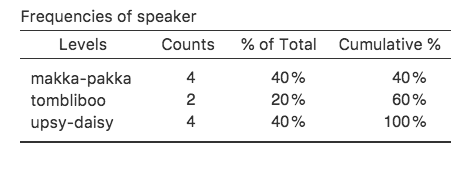
\includegraphics[width=1\linewidth]{img/mechanics/freqtable} 

}

\caption{Frequency table for the **`speaker`** variable}\label{fig:freqtable}
\end{figure}

The output here tells us on the first line that what we're looking at is a tabulation of the \textbf{\texttt{speaker}} variable. In the `Levels' column it lists all the different speakers that exist in the data, and in the `Counts' column it tells you how many times that speaker appears in the data. In other words, it's a frequency table.

In jamovi, the `Frequency tables' check box will only produce a table for single variables. For a table of two variables, for example combining \textbf{\texttt{speaker}} and \textbf{\texttt{utterance}} so that we can see how many times each speaker said a particular utterance, we need a cross-tabulation or contingency table. In jamovi you can do this by selecting the `Frequencies' - `Contingency Tables' - `Independent Samples' analysis, and moving the \textbf{\texttt{speaker}} variable into the `Rows' box, and the \textbf{\texttt{utterance}} variable into the `Columns' box. You then should have a contingency table like the one shown in Figure \ref{fig:contingencytable}.

\begin{figure}

{\centering 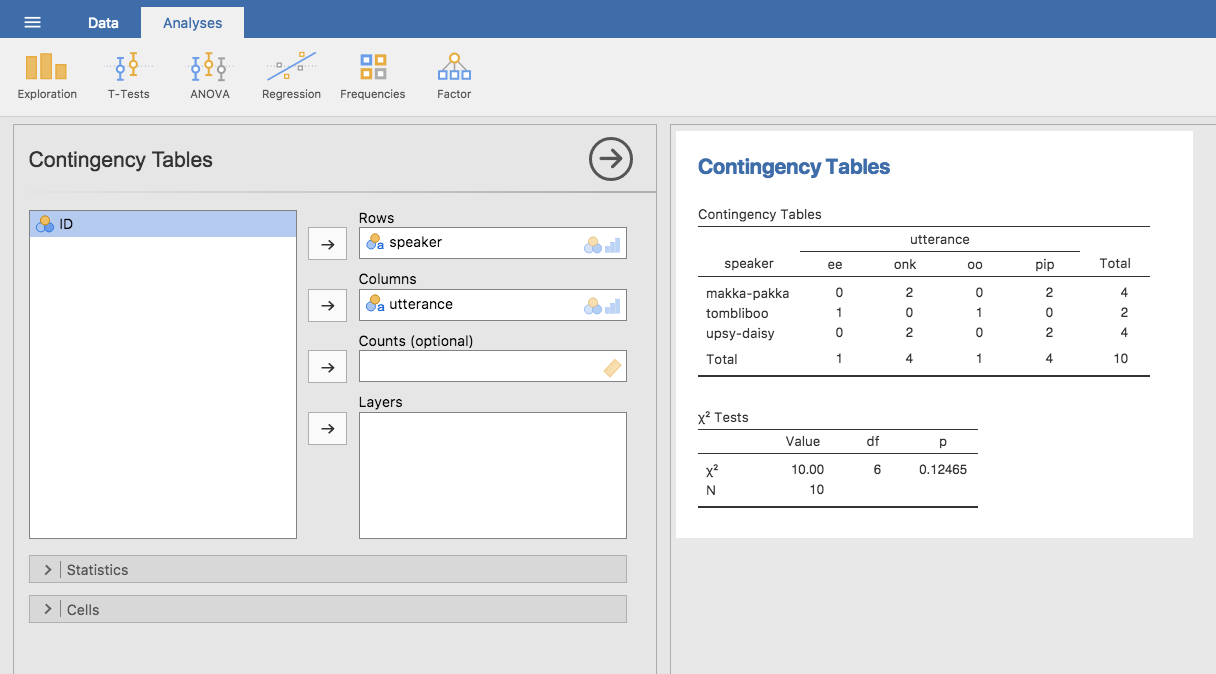
\includegraphics[width=1\linewidth]{img/mechanics/contingencytable} 

}

\caption{Contingency table for the **`speaker`** and **`utterance`** variables}\label{fig:contingencytable}
\end{figure}

Don't worry about the ``\(\chi^2\) Tests'' table that is produced. We are going to cover this later on in Chapter \ref{chisquare}. When interpreting the contingency table remember that these are counts, so the fact that the first row and second column of numbers corresponds to a value of 2 indicates that Makka-Pakka (row 1) says `onk' (column 2) twice in this data set.

\hypertarget{adding-percentages-to-a-contingency-table}{%
\subsection{Adding percentages to a contingency table}\label{adding-percentages-to-a-contingency-table}}

The contingency table shown in Figure \ref{fig:contingencytable} shows a table of raw frequencies. That is, a count of the total number of cases for different combinations of levels of the specified variables. However, often you want your data to be organised in terms of percentages as well as counts. You can find the check boxes for different percentages under the `Cells' option in the `Contingency Tables' window. First, click on the `Row' check box and the Contingency Table in the output window will change to the one in Figure \ref{fig:contingencyrow}.

\begin{figure}

{\centering 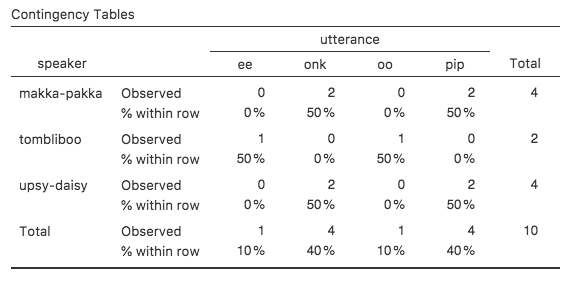
\includegraphics[width=1\linewidth]{img/mechanics/contingencyrow} 

}

\caption{Contingency table for the **`speaker`** and **`utterance`** variables, with row percentages}\label{fig:contingencyrow}
\end{figure}

\begin{figure}

{\centering 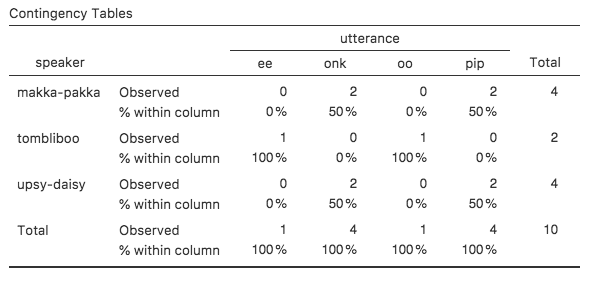
\includegraphics[width=1\linewidth]{img/mechanics/contingencycol} 

}

\caption{Contingency table for the **`speaker`** and **`utterance`** variables, with column percentages}\label{fig:contingencycol}
\end{figure}

What we're looking at here is the percentage of utterances made by each character. In other words, 50\% of Makka-Pakka's utterances are `pip,' and the other 50\% are onk'. Let's contrast this with the table we get when we calculate column percentages (uncheck `Row' and check `Column' in the Cells options window), see Figure \ref{fig:contingencycol}. In this version, what we're seeing is the percentage of characters associated with each utterance. For instance, whenever the utterance `ee' is made (in this data set), 100\% of the time it's a Tombliboo saying it.

\hypertarget{logicals}{%
\section{Logical expressions in jamovi}\label{logicals}}

A key concept that a lot of data transformations in jamovi rely on is the idea of a {\textbf{logical value}}. A logical value is an assertion about whether something is true or false. This is implemented in jamovi in a pretty straightforward way. There are two logical values, namely \texttt{TRUE} and \texttt{FALSE}. Despite the simplicity, logical values are very useful things. Let's see how they work.

\hypertarget{assessing-mathematical-truths}{%
\subsection{Assessing mathematical truths}\label{assessing-mathematical-truths}}

In George Orwell's classic book \emph{1984} one of the slogans used by the totalitarian Party was `two plus two equals five.' The idea being that the political domination of human freedom becomes complete when it is possible to subvert even the most basic of truths. It's a terrifying thought, especially when the protagonist Winston Smith finally breaks down under torture and agrees to the proposition. `Man is infinitely malleable,' the book says. I'm pretty sure that this isn't true of humans\footnote{I offer up my teenage attempts to be ``cool'' as evidence that some things just can't be done.} and it's definitely not true of jamovi. jamovi is not infinitely malleable, it has rather firm opinions on the topic of what is and isn't true, at least as regards basic mathematics. If I ask it to calculate \texttt{2\ +\ 2}\footnote{You can do this in the Compute new variable screen, though just calculating \texttt{2\ +\ 2} for every cell of a new variable is not very useful!}, it always gives the same answer, and it's not bloody 5!

Of course, so far jamovi is just doing the calculations. I haven't asked it to explicitly assert that \(2+2 = 4\) is a true statement. If I want jamovi to make an explicit judgement, I can use a command like this: \texttt{2\ +\ 2\ ==\ 4}

What I've done here is use the {\textbf{equality operator}}, \texttt{==}, to force jamovi to make a ``true or false'' judgement.\footnote{Note that this is a very different operator to the equals operator \texttt{=}. A common typo that people make when trying to write logical commands in jamovi (or other languages, since the \texttt{=} versus \texttt{==} distinction is important in many computer and statistical programs) is to accidentally type \texttt{=} when you really mean \texttt{==}. Be especially cautious with this, I've been programming in various languages since I was a teenager and I \emph{still} screw this up a lot. Hmm. I think I see why I wasn't cool as a teenager. And why I'm still not cool.} Okay, let's see what jamovi thinks of the Party slogan, so type this into the compute new variable `formula' box:

\texttt{2\ +\ 2\ ==\ 5}

And what do you get? It should be a whole set of `false' values in the spreadsheet column for your newly computed variable. Booyah! Freedom and ponies for all! Or something like that. Anyway, it was worth having a look at what happens if I try to \emph{force} jamovi to believe that two plus two is five by making a statement like \texttt{2\ +\ 2\ =\ 5}. I know that if I do this in another program, say R, then it throws up an error message. But wait, if you do this in jamovi you get a whole set of `false' values. So what is going on? Well, it seems that jamovi is being pretty smart and realises that you are testing whether it is TRUE or FALSE that \texttt{2\ +\ 2\ =\ 5}, regardless of whether you use the correct {\textbf{equality operator}}, \texttt{==}, or the equals sign \texttt{=}.

\hypertarget{logical-operations}{%
\subsection{Logical operations}\label{logical-operations}}

So now we've seen logical operations at work. But so far we've only seen the simplest possible example. You probably won't be surprised to discover that we can combine logical operations with other operations and functions in a more complicated way, like this:

\texttt{3*3\ +\ 4*4\ ==\ 5*5}

or this

\texttt{SQRT(25)\ ==\ 5}

Not only that, but as Table \ref{tab:logicaltab} illustrates, there are several other logical operators that you can use corresponding to some basic mathematical concepts. Hopefully these are all pretty self-explanatory. For example, the {\textbf{less than}} operator \texttt{\textless{}} checks to see if the number on the left is less than the number on the right. If it's less, then jamovi returns an answer of \texttt{TRUE}, but if the two numbers are equal, or if the one on the right is larger, then jamovi returns an answer of \texttt{FALSE}.

In contrast, the {\textbf{less than or equal to}} operator \texttt{\textless{}=} will do exactly what it says. It returns a value of \texttt{TRUE} if the number of the left hand side is less than or equal to the number on the right hand side. At this point I hope it's pretty obvious what the {\textbf{greater than}} operator \texttt{\textgreater{}} and the {\textbf{greater than or equal to}} operator \texttt{\textgreater{}=} do!

Next on the list of logical operators is the {\textbf{not equal to}} operator \texttt{!=} which, as with all the others, does what it says it does. It returns a value of \texttt{TRUE} when things on either side are not identical to each other. Therefore, since \(2+2\) isn't equal to \(5\), we would get `true' as the value for our newly computed variable. Try it and see:

\texttt{2\ +\ 2\ !=\ 5}

\begin{table}

\caption{\label{tab:logicaltab}Some logical operators. Technically I should be calling these "binary relational operators", but quite frankly I don't want to. It's my book so no-one can make me.}
\centering
\begin{tabular}[t]{llll}
\toprule
operation & operator & example input & answer\\
\midrule
less than & < & 2 < 3 & `TRUE`\\
less than or equal to & <= & 2 <= 2 & `TRUE`\\
greater than & > & 2 > 3 & `FALSE`\\
greater than or equal to & >= & 2 >= 2 & `TRUE`\\
equal to & == & 2 == 3 & `FALSE`\\
\addlinespace
not equal to & != & 2 != 3 & `TRUE`\\
\bottomrule
\end{tabular}
\end{table}

We're not quite done yet. There are three more logical operations that are worth knowing about, listed in Table \ref{tab:logicals2}. These are the {\textbf{not}} operator \texttt{!}, the {\textbf{and}} operator \texttt{and}, and the {\textbf{or}} operator \texttt{or}. Like the other logical operators, their behaviour is more or less exactly what you'd expect given their names. For instance, if I ask you to assess the claim that `either \(2+2 = 4\) \emph{or} \(2+2 = 5\)' you'd say that it's true. Since it's an `either-or' statement, all we need is for one of the two parts to be true. That's what the \texttt{or} operator does:\footnote{Now, here's a quirk in jamovi. When you have simple logical expressions like the ones we have already met, e.g.~\texttt{2\ +\ 2\ ==\ 5} then jamovi neatly states `false' (or `true') in the corresponding spreadsheet column. Underneath the hood, jamovi stores `false' as \texttt{0} and `true' as \texttt{1}. When we have more complex logical expressions, such as \texttt{(2+2\ ==\ 4)\ or\ (2+2\ ==\ 5)}, then jamovi just displays either \texttt{0} or \texttt{1}, depending whether the logical expression is evaluated as false, or true.}

\texttt{(2+2\ ==\ 4)\ or\ (2+2\ ==\ 5)}

On the other hand, if I ask you to assess the claim that `both \(2+2 = 4\) \emph{and} \(2+2 = 5\)' you'd say that it's false. Since this is an \emph{and} statement we need both parts to be true. And that's what the \texttt{and} operator does:

\texttt{(2+2\ ==\ 4)\ and\ (2+2\ ==\ 5)}

Finally, there's the \emph{not} operator, which is simple but annoying to describe in English. If I ask you to assess my claim that `it is not true that \(2+2 = 5\)' then you would say that my claim is true, because actually my claim is that ``\(2+2 = 5\) is false.'' And I'm right. If we write this in jamovi we use this:

\texttt{NOT(2+2\ ==\ 5)}

In other words, since \texttt{2+2\ ==\ 5} is a \texttt{FALSE} statement, it must be the case that \texttt{NOT(2+2\ ==\ 5)} is a \texttt{TRUE} one. Essentially, what we've really done is claim that ``not false'' is the same thing as ``true.'' Obviously, this isn't really quite right in real life. But jamovi lives in a much more black or white world. For jamovi everything is either true or false. No shades of grey are allowed.

Of course, in our \(2+2 = 5\) example, we didn't really need to use the `not' operator \texttt{NOT} and the ``equals to'' operator \texttt{==} as two separate operators. We could have just used the `not equals to' operator \texttt{!=} like this:

\texttt{2+2\ !=\ 5}

\begin{table}

\caption{\label{tab:logicals2}Some more logical operators.}
\centering
\begin{tabular}[t]{llll}
\toprule
operation & operator & example input & answer\\
\midrule
not & NOT & NOT(1==1) & `FALSE`\\
or & or & (1==1) or (2==3) & `TRUE`\\
and & and & (1==1) and (2==3) & `FALSE`\\
\bottomrule
\end{tabular}
\end{table}

\hypertarget{logictext}{%
\subsection{Applying logical operation to text}\label{logictext}}

I also want to briefly point out that you can apply these logical operators to text as well as to logical data. It's just that we need to be a bit more careful in understanding how jamovi interprets the different operations. In this section I'll talk about how the equal to operator \texttt{==} applies to text, since this is the most important one. Obviously, the not equal to operator \texttt{!=} gives the exact opposite answers to \texttt{==} so I'm implicitly talking about that one too, but I won't give specific commands showing the use of \texttt{!=}.

Okay, let's see how it works. In one sense, it's very simple. For instance, I can ask jamovi if the word \texttt{"cat"} is the same as the word \texttt{"dog"}, like this:

\texttt{"cat"\ ==\ "dog"}

That's pretty obvious, and it's good to know that even jamovi can figure that out. Similarly, jamovi does recognise that a \texttt{"cat"\ is\ a}``cat''`

\texttt{"cat"\ ==\ "cat"}

Again, that's exactly what we'd expect. However, what you need to keep in mind is that jamovi is not at all tolerant when it comes to grammar and spacing. If two strings differ in any way whatsoever, jamovi will say that they're not equal to each other, as with the following:

\texttt{"\ cat"\ ==\ "cat"}
\texttt{"cat"\ ==\ "CAT"}
\texttt{"cat"\ ==\ "c\ a\ t"}

You can also use other logical operators too. For instance jamovi also allows you to use the \texttt{\textless{}} and \texttt{\textgreater{}} operators to determine which of two text `strings' comes first, alphabetically speaking. Sort of. Actually, it's a bit more complicated than that, but let's start with a simple example:

\texttt{"cat"\ \textless{}\ "dog"}

In jamovi, this example evaluates to `true.' This is because \texttt{"cat"} does does come before \texttt{"dog"} alphabetically, so jamovi judges the statement to be true. However, if we ask jamovi to tell us if \texttt{"cat"} comes before \texttt{"anteater"} then it will evaluate the expression as false. So far, so good. But text data is a bit more complicated than the dictionary suggests. What about \texttt{"cat"} and \texttt{"CAT"}? Which of these comes first? Try it and find out:

\texttt{"CAT"\ \textless{}\ "cat"}

This in fact evaluates to `true.' In other words, jamovi assumes that uppercase letters come before lowercase ones. Fair enough. No-one is likely to be surprised by that. What you might find surprising is that jamovi assumes that \emph{all} uppercase letters come before \emph{all} lowercase ones. That is, while \texttt{"anteater"\ \textless{}\ "zebra"} is a true statement, and the uppercase equivalent \texttt{"ANTEATER"\ \textless{}\ "ZEBRA"} is also true, it is \emph{not} true to say that \texttt{"anteater"\ \textless{}\ "ZEBRA"}, as the following extract illustrates. Try this:

\texttt{"anteater"\ \textless{}\ "ZEBRA"}

This evaluates to `false,' and this may seem slightly counterintuitive. With that in mind, it may help to have a quick look at Table \ref{tab:asciiorder} which lists various text characters in the order that jamovi processes them.

\begin{table}

\caption{\label{tab:asciiorder}The ordering of various text characters used by the < and > operators. Not shown is the “space” character, which actually comes <U+FB01>rst on the list.}
\centering
\begin{tabular}[t]{l}
\hline
Characters\\
\hline
! " \# \$ \% \& ’ ( ) * + , - . / 0 1 2 3 4 5 6 7 8 9 : ; < = > ? @ A B C D E F G H I J K L M N O P Q R S T U V W X Y Z [  ] \textasciicircum{} \_ ‘ a b c d e f g h i j k l m n o p q r s t u v w x y z \} | \{\\
\hline
\end{tabular}
\end{table}

\hypertarget{transform}{%
\section{Transforming and recoding a variable}\label{transform}}

It's not uncommon in real world data analysis to find that one of your variables isn't quite equivalent to the variable that you really want. For instance, it's often convenient to take a continuous-valued variable (e.g., age) and break it up into a smallish number of categories (e.g., younger, middle, older). At other times, you may need to convert a numeric variable into a different numeric variable (e.g., you may want to analyse at the absolute value of the original variable). In this section I'll describe a few key ways you can do these things in jamovi.

\hypertarget{creating-a-transformed-variable}{%
\subsection{Creating a transformed variable}\label{creating-a-transformed-variable}}

The first trick to discuss is the idea of {\textbf{transforming}} a variable. Taken literally, \emph{anything} you do to a variable is a transformation, but in practice what it usually means is that you apply a relatively simple mathematical function to the original variable in order to create a new variable that either (a) provides a better way of describing the thing you're actually interested in, or (b) is more closely in agreement with the assumptions of the statistical tests you want to do. Since, at this stage, I haven't talked about statistical tests or their assumptions, I'll show you an example based on the first case.

Suppose I've run a short study in which I ask 10 people a single question:

\begin{quote}
On a scale of 1 (strongly disagree) to 7 (strongly agree), to what extent do you agree with the proposition that ``Dinosaurs are awesome?''
\end{quote}

Now let's load and look at the data. The data file \textbf{\texttt{likert.omv}} contains a single variable that contains raw Likert-scale responses for these 10 people. However, if you think about it, this isn't the best way to represent these responses. Because of the fairly symmetric way that we set up the response scale, there's a sense in which the midpoint of the scale should have been coded as 0 (no opinion), and the two endpoints should be \(+3\) (strongly agree) and \(-3\) (strongly disagree). By recoding the data in this way it's a bit more reflective of how we really think about the responses. The recoding here is pretty straightforward, we just subtract 4 from the raw scores. In jamovi you can do this by computing a new variable: click on the `Data' - `Compute' button and you will see that a new variable has been added to the spreadsheet. Let's call this new variable \textbf{\texttt{likert.centred}} (go ahead and type that in) and then add the following in the formula box, like in Figure \ref{fig:likertraw}: `\textbf{\texttt{likert.raw\ -\ 4}}'

\begin{figure}

{\centering 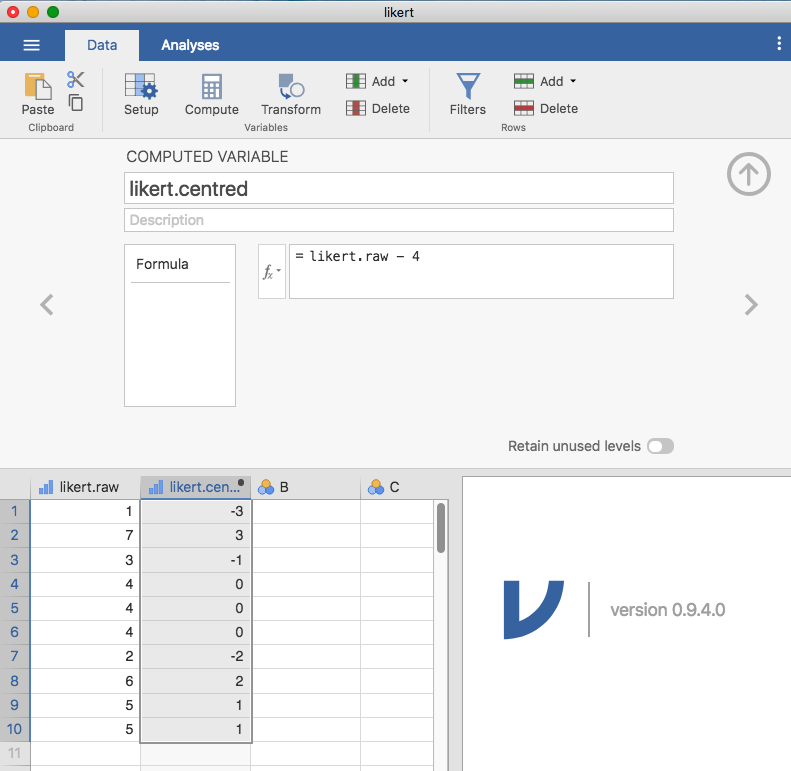
\includegraphics[width=1\linewidth]{img/mechanics/likertraw} 

}

\caption{Creating a new computed variable in jamovi}\label{fig:likertraw}
\end{figure}

One reason why it might be useful to have the data in this format is that there are a lot of situations where you might prefer to analyse the \emph{strength} of the opinion separately from the \emph{direction} of the opinion. We can do two different transformations on this \textbf{\texttt{likert.centred}} variable in order to distinguish between these two different concepts. First, to compute an \textbf{\texttt{opinion.strength}} variable, we want to take the absolute value of the centred data (using the `ABS' function).\footnote{The absolute value of a number is its distance from zero, regardless of whether it's sign is negative or positive.} In jamovi, create another new variable using the `Compute' button. Name the variable \textbf{\texttt{opinion.strength}} and this time click on the \emph{\(f\)\textsubscript{x}} button next to the `Formula' box. This shows the different `Functions' and `Variables' that you can add to the `Formula' box, so double click on `ABS' and then double click on `likert.centred' and you will see that the `Formula' box is populated with ABS(likert.centred) and a new variable has been created in the spreadsheet view, as in Figure \ref{fig:opinionstrength}

\begin{figure}

{\centering 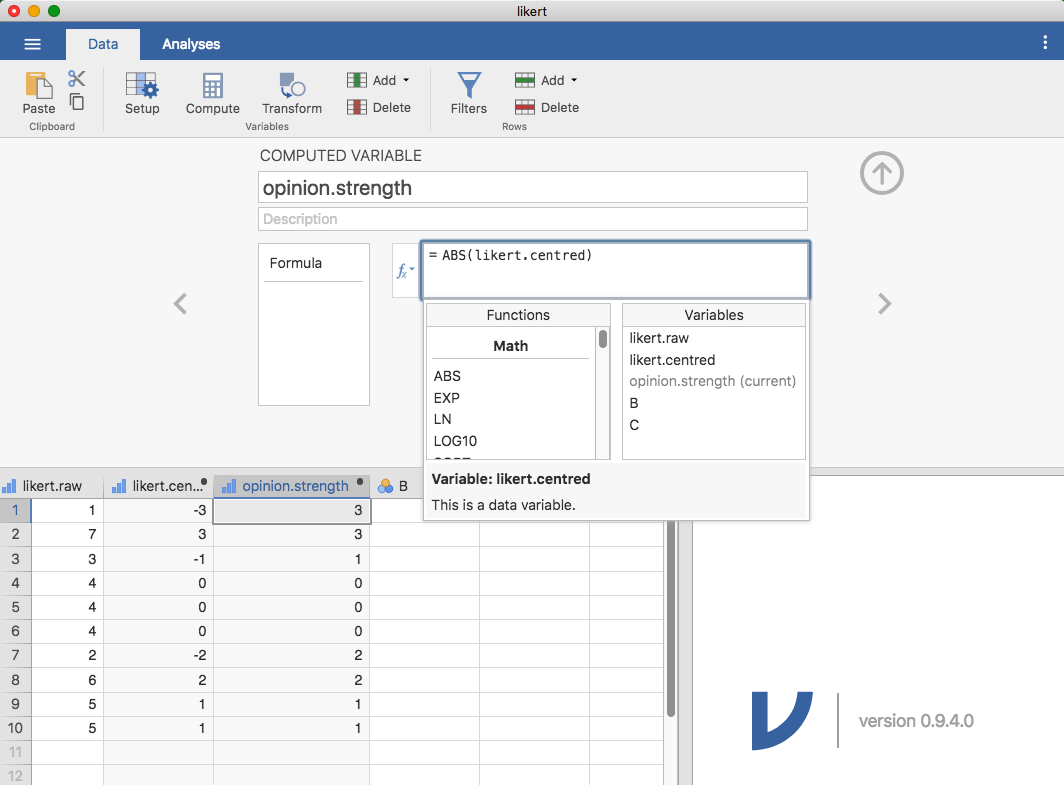
\includegraphics[width=1\linewidth]{img/mechanics/opinionstrength} 

}

\caption{Using the *$f$~x~* button to select functions and variables}\label{fig:opinionstrength}
\end{figure}

Second, to compute a variable that contains only the direction of the opinion and ignores the strength, we want to calculate the `sign' of the variable. In jamovi we can use the `IF' function to do this. Create another new variable using the `Compute' button, name this one \textbf{\texttt{opinion.sign}}, and then type the following into the function box:

\texttt{IF(likert.centred\ ==\ 0,\ 0,\ likert.centred\ /\ opinion.strength)}

When done, you'll see that all negative numbers from the \textbf{\texttt{likert.centred}} variable are converted to \(-1\), all positive numbers are converted to \(1\) and zero stays as \(0\), like so:

\texttt{-1\ \ 1\ -1\ \ 0\ \ 0\ \ 0\ -1\ \ 1\ \ 1\ \ 1}

Let's break down what this `IF' command is doing. In jamovi there are three parts to an `IF' statement, written as `IF(expression, value, else).' The first part, `expression' can be a logical or mathematical statement. In our example, we have specified `likert.centred == 0,' which is TRUE for values where likert.centred is zero. The next part, `value,' is the new value where the expression in part one is TRUE. In our example, we have said that for all those values where likert.centred is zero, keep them zero. In the next part, `else,' we can enter another logical or mathematical statement to be used if part one evaluates to FALSE, i.e.~where \textbf{\texttt{likert.centred}} is not zero. In our example we have divided likert.centred by opinion.strength to give `-1' or `+1' depending of the sign of the original value in likert.centred.\footnote{The reason we have to use the `IF' command and keep zero as zero is that you cannot just use likert.centred / opinion.strength to calculate the sign of likert.centred, because mathematically dividing zero by zero does not work. Try it and see}

And we're done. We now have three shiny new variables, all of which are useful transformations of the original \textbf{\texttt{likert.raw}} data.

\hypertarget{collapsing-a-variable-into-a-smaller-number-of-discrete-levels-or-categories}{%
\subsection{Collapsing a variable into a smaller number of discrete levels or categories}\label{collapsing-a-variable-into-a-smaller-number-of-discrete-levels-or-categories}}

One pragmatic task that comes up quite often is the problem of collapsing a variable into a smaller number of discrete levels or categories. For instance, suppose I'm interested in looking at the age distribution of people at a social gathering:

\texttt{60,58,24,26,34,42,31,30,33,2,9}

In some situations it can be quite helpful to group these into a smallish number of categories. For example, we could group the data into three broad categories: young (0-20), adult (21-40) and older (41-60). This is a quite coarse-grained classification, and the labels that I've attached only make sense in the context of this data set (e.g., viewed more generally, a 42 year old wouldn't consider themselves as `older'). We can slice this variable up quite easily using the jamovi `IF' function that we have already used. This time we have to specify nested `IF' statements, meaning simply that IF the first logical expression is TRUE, insert a first value, but IF a second logical expression is TRUE, insert a second value, but IF a third logical expression is TRUE, then insert a third value. This can be written as:

\begin{verbatim}
IF(Age >= 0 and Age <= 20, 1,
IF(Age >= 21 and Age <= 40, 2,
IF(Age >= 41 and Age <= 60, 3 )))
\end{verbatim}

Note that there are three left parentheses used during the nesting, so the whole statement has to end with three right parentheses otherwise you will get an error message. The jamovi screen shot for this data manipulation, along with an accompanying frequency table, is shown in Figure \ref{fig:agecats}

\begin{figure}

{\centering 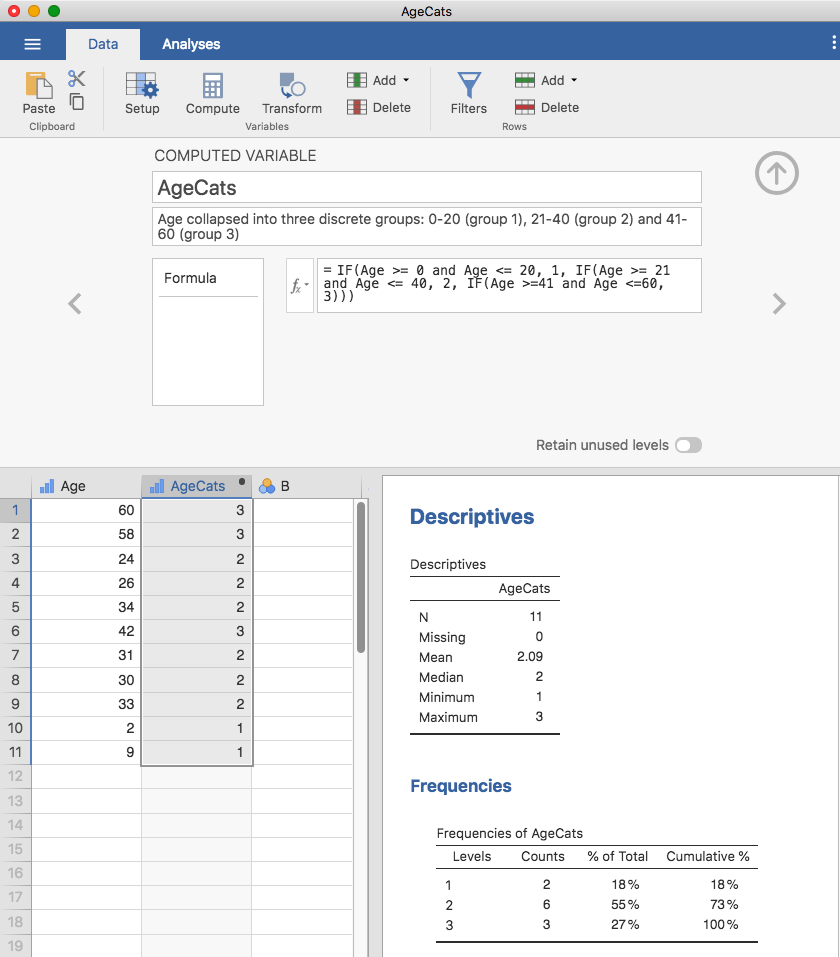
\includegraphics[width=1\linewidth]{img/mechanics/agecats} 

}

\caption{Collapsing a variable into a smaller number of discrete levels using the jamovi 'IF' function}\label{fig:agecats}
\end{figure}

It's important to take the time to figure out whether or not the resulting categories make any sense at all in terms of your research project. If they don't make any sense to you as meaningful categories, then any data analysis that uses those categories is likely to be just as meaningless. More generally, in practice I've noticed that people have a very strong desire to carve their (continuous and messy) data into a few (discrete and simple) categories, and then run analyses using the categorised data instead of the original data.\footnote{If you've read further into the book, and are re-reading this section, then a good example of this would be someone choosing to do an ANOVA using \texttt{AgeCats} as the grouping variable, instead of running a regression using \texttt{Age} as a predictor. There are sometimes good reasons for doing this. For instance, if the relationship between \texttt{Age} and your outcome variable is highly non-linear and you aren't comfortable with trying to run non-linear regression! However, unless you really do have a good rationale for doing this, it's best not to. It tends to introduce all sorts of other problems (e.g., the data will probably violate the normality assumption) and you can lose a lot of statistical power.} I wouldn't go so far as to say that this is an inherently bad idea, but it does have some fairly serious drawbacks at times, so I would advise some caution if you are thinking about doing it.

\hypertarget{creating-a-transformation-that-can-be-applied-to-multiple-variables}{%
\subsection{Creating a transformation that can be applied to multiple variables}\label{creating-a-transformation-that-can-be-applied-to-multiple-variables}}

Sometimes you want to apply the same transformation to more than one variable, for example when you have multiple questionnaire items that all need to be recalculated or recoded in the same way. And one of the neat features in jamovi is that you can create a transformation, using the `Data' - `Transform' button, that can then be saved and applied to multiple variables. Let's go back to the first example above, using the data file \textbf{\texttt{likert.omv}} that contains a single variable with raw Likert-scale responses for 10 people. To create a transformation that you can save and then apply across multiple variables (assuming you had more variables like this in your data file), first in the spreadsheet editor select (i.e., click) the variable you want to use to initially create the transformation. In our example this is \textbf{\texttt{likert.raw}}. Next click the `Transform' button in the jamovi `Data' ribbon, and you'll see something like Figure \ref{fig:transform1}.

\begin{figure}

{\centering 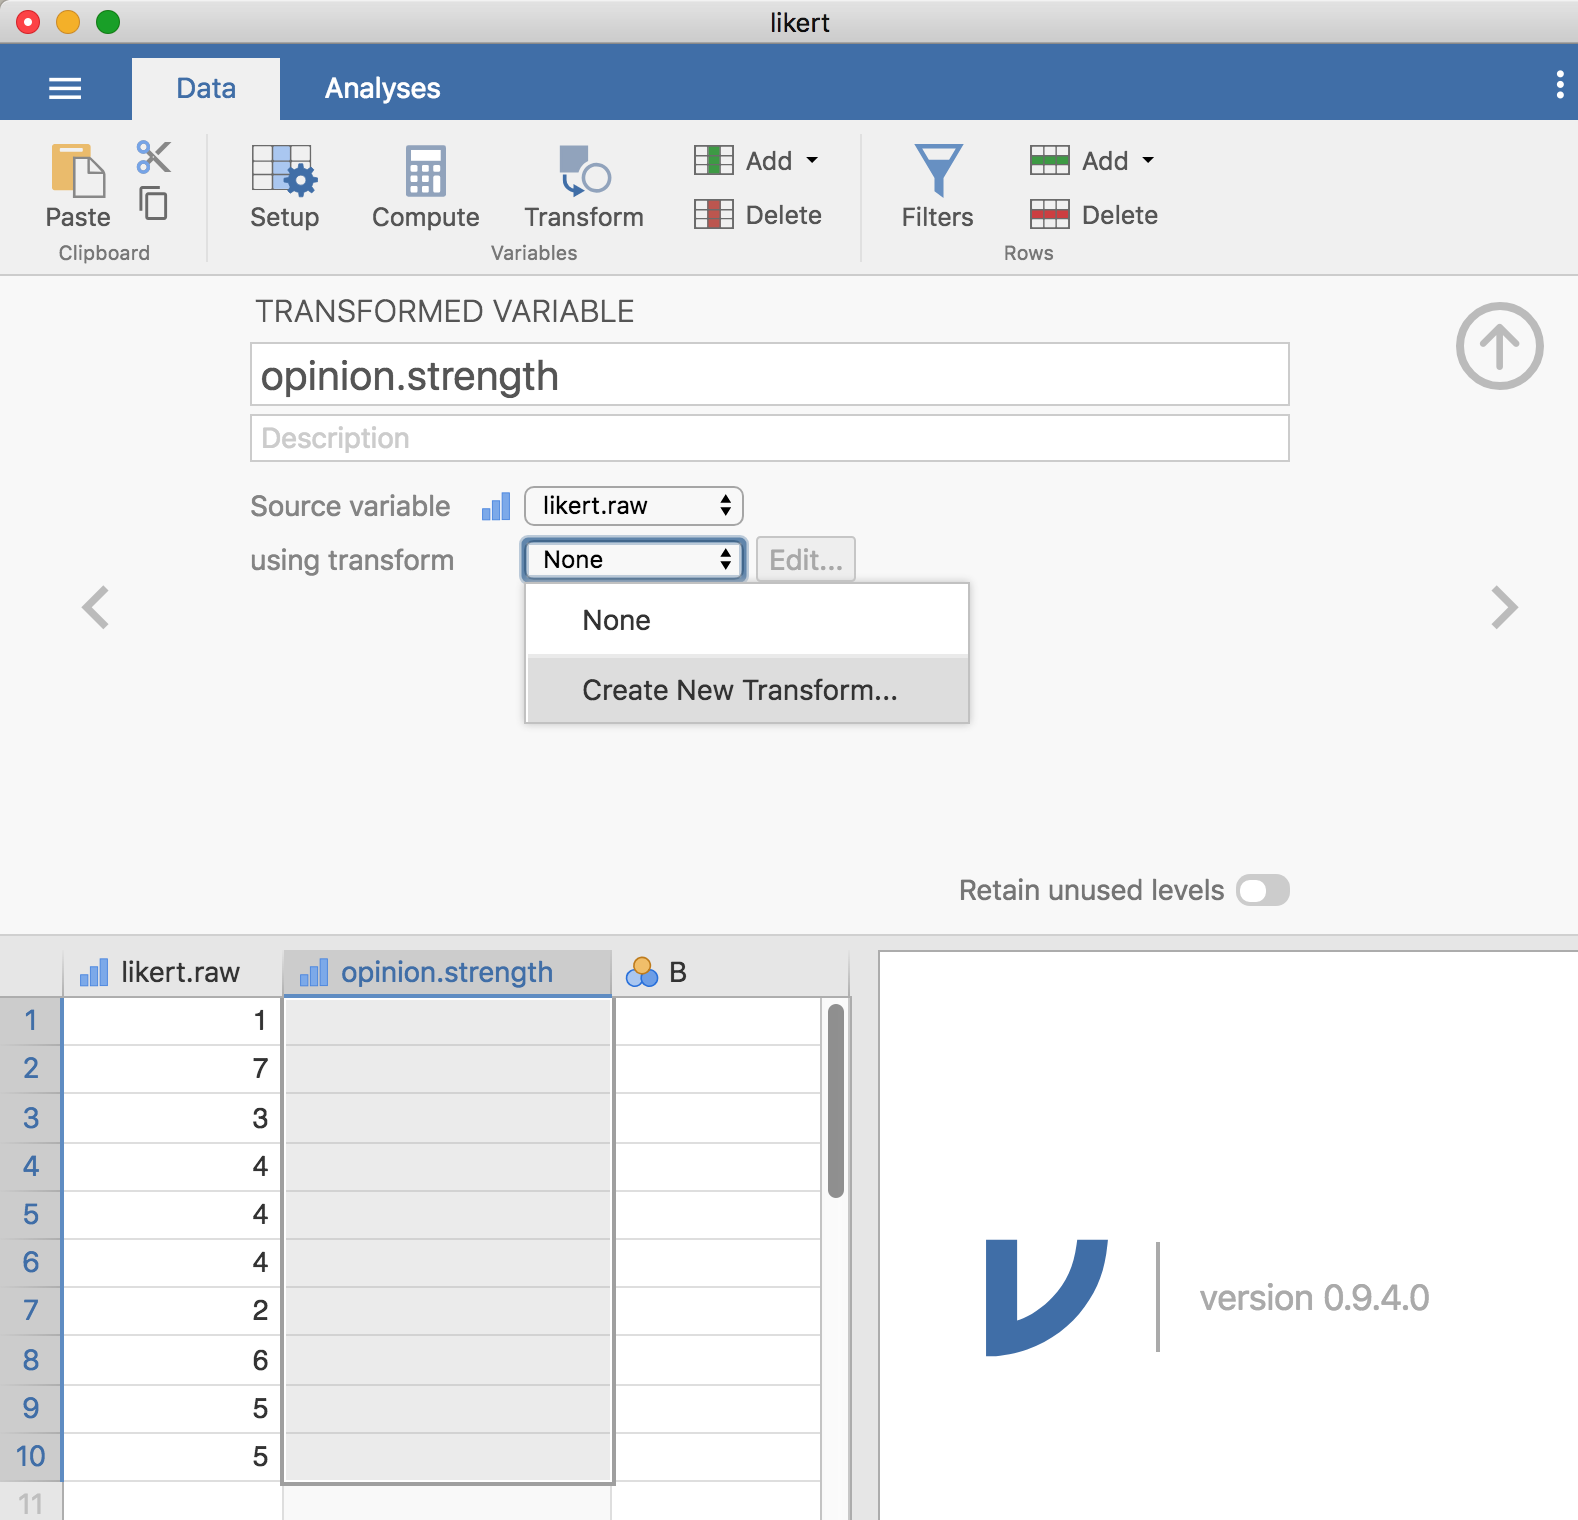
\includegraphics[width=1\linewidth]{img/mechanics/transform1} 

}

\caption{Creating a new variable transformation using the jamovi 'Transform' command}\label{fig:transform1}
\end{figure}

Give your new variable a name, let's call it \textbf{\texttt{opinion.strength}} and then click on the `using transform' selection box and select `Create New Transform\ldots{}.' This is where you will create, and name, the transformation that can be re-applied to as many variables as you like. The transformation is automatically named for us as `Transform 1' (imaginative, huh. You can change this if you like). Then type the expression `\texttt{ABS(\$source\ -\ 4)}' into the function text box, as in Figure \ref{fig:transform2}, press Enter or Return on your keyboard and, hey presto, you have created a new transformation and applied it to the \textbf{\texttt{likert.raw}} variable! Good, eh. Note that instead of using the variable label in the expression, we have instead used \textbf{\texttt{\$source}}. This is so that we can then use the same transformation with as many different variables as we like - jamovi requires you to use \textbf{\texttt{\$source}} to refer to the source variable you are transforming. Your transformation has also been saved and can be re-used any time you like (providing you save the dataset as an `.omv' file, otherwise you'll lose it!).

\begin{figure}

{\centering 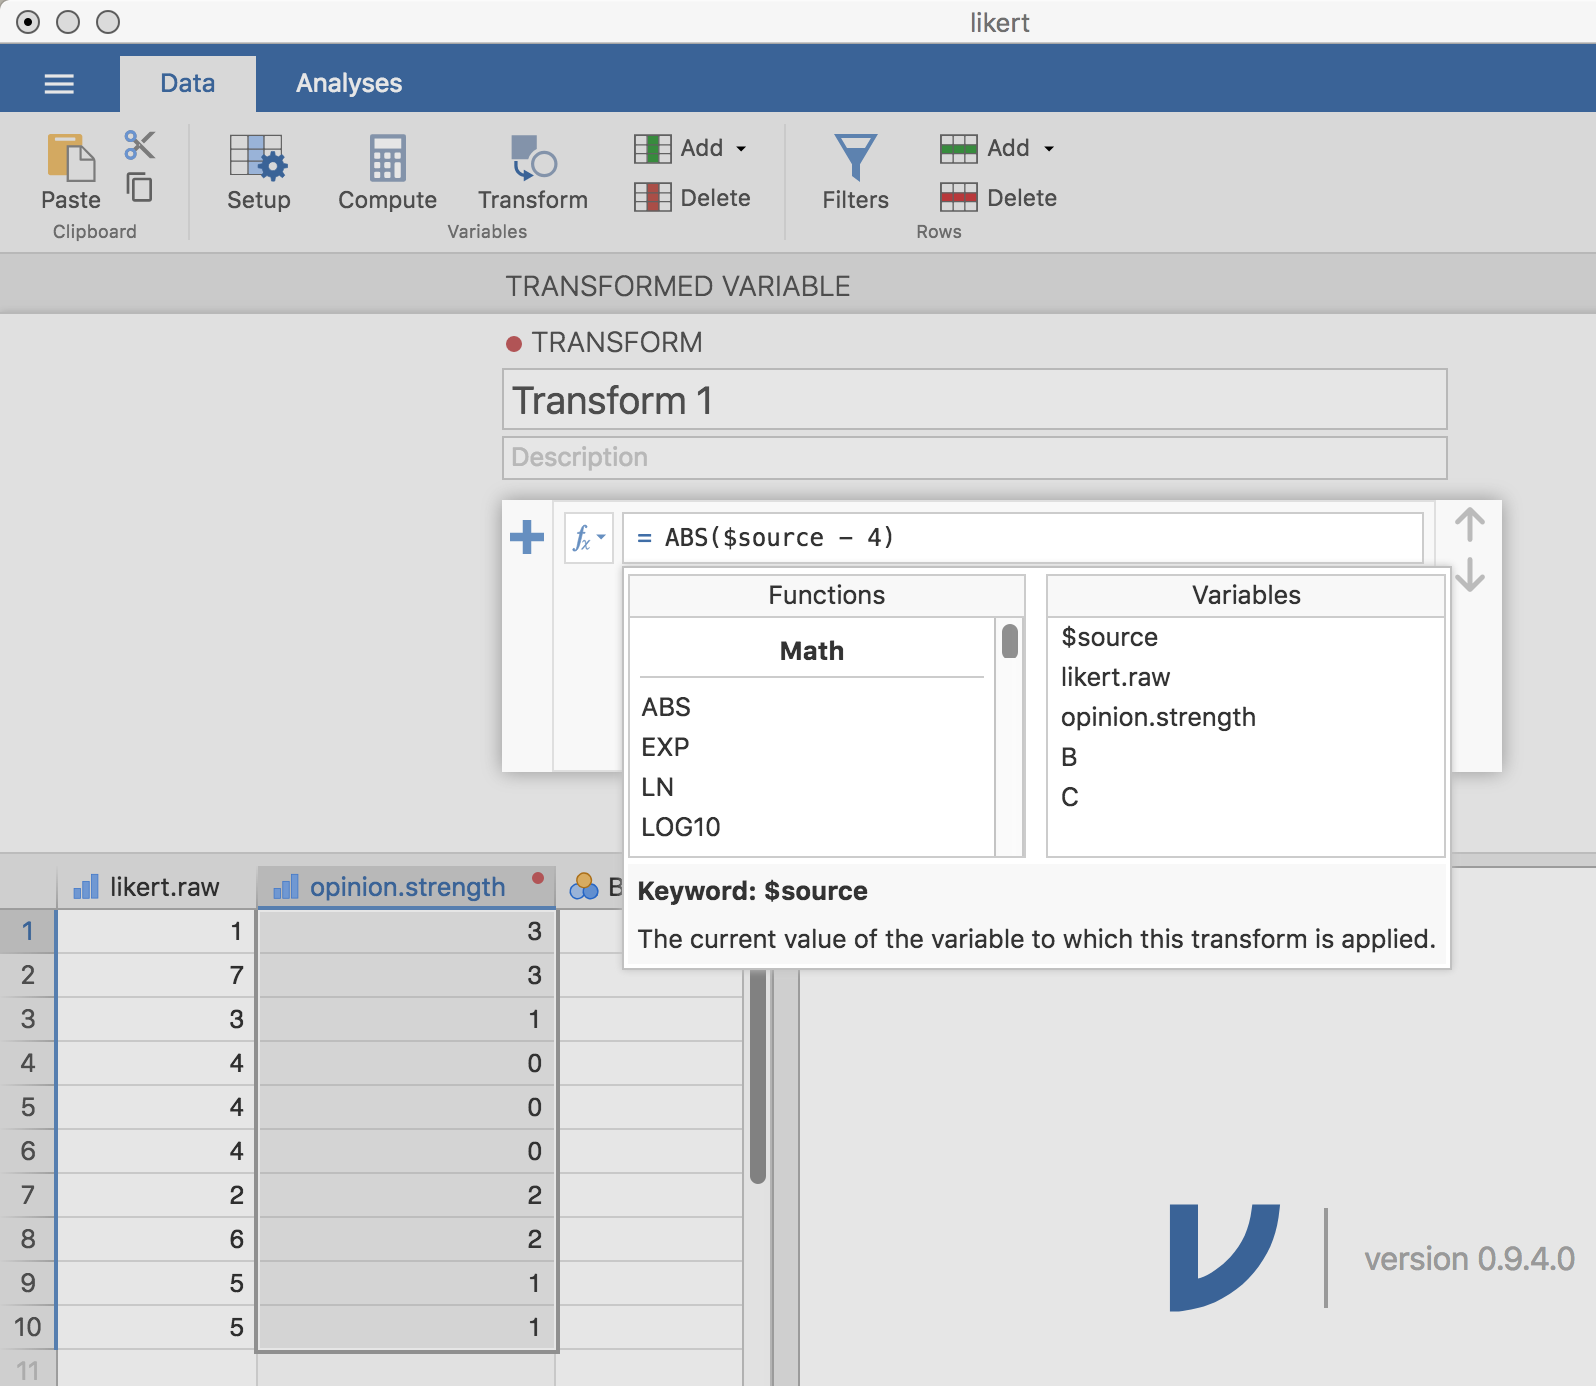
\includegraphics[width=1\linewidth]{img/mechanics/transform2} 

}

\caption{Specifying a transformation in jamovi, to be saved as the imaginatively named 'Transform 1'}\label{fig:transform2}
\end{figure}

You can also create a transformation with the second example we looked at, the age distribution of people at a social gathering. Go on, you know you want to! Remember that we collapsed this variable into three groups: younger, adult and older. This time we will achieve the same thing, but using the jamovi `Transform' - `Add condition' button. With this data set (go back to it or create it again if you didn't save it) set up a new variable transformation. Call the transformed variable \texttt{AgeCats} and the transformation you will create \textbf{\texttt{Agegroupings}}. Then click on the big ``+'' sign next to the function box. This is the `Add condition' button and I've stuck a big red arrow onto Figure \ref{fig:transform3} so you can see exactly where this is. Re-create the transformation shown in Figure \ref{fig:transform3} and when you have done, you will see the new values appear in the spreadsheet window. What's more, the \texttt{Agegroupings} transformation has been saved and can be re-applied any time you like. Ok, so I know that it's unlikely you will have more than one `Age' variable, but you get the idea now of how to set up transformations in jamovi, so you can follow this idea with other sorts of variables. A typical scenario for this is when you have a questionnaire scale with, say, 20 items (variables) and each item was originally scored from 1 to 6 but, for some reason or quirk of the data you decide to recode all the items as 1 to 3. You can easily do this in jamovi by creating and then re-applying your transformation for each variable that you want to recode.

\begin{figure}

{\centering 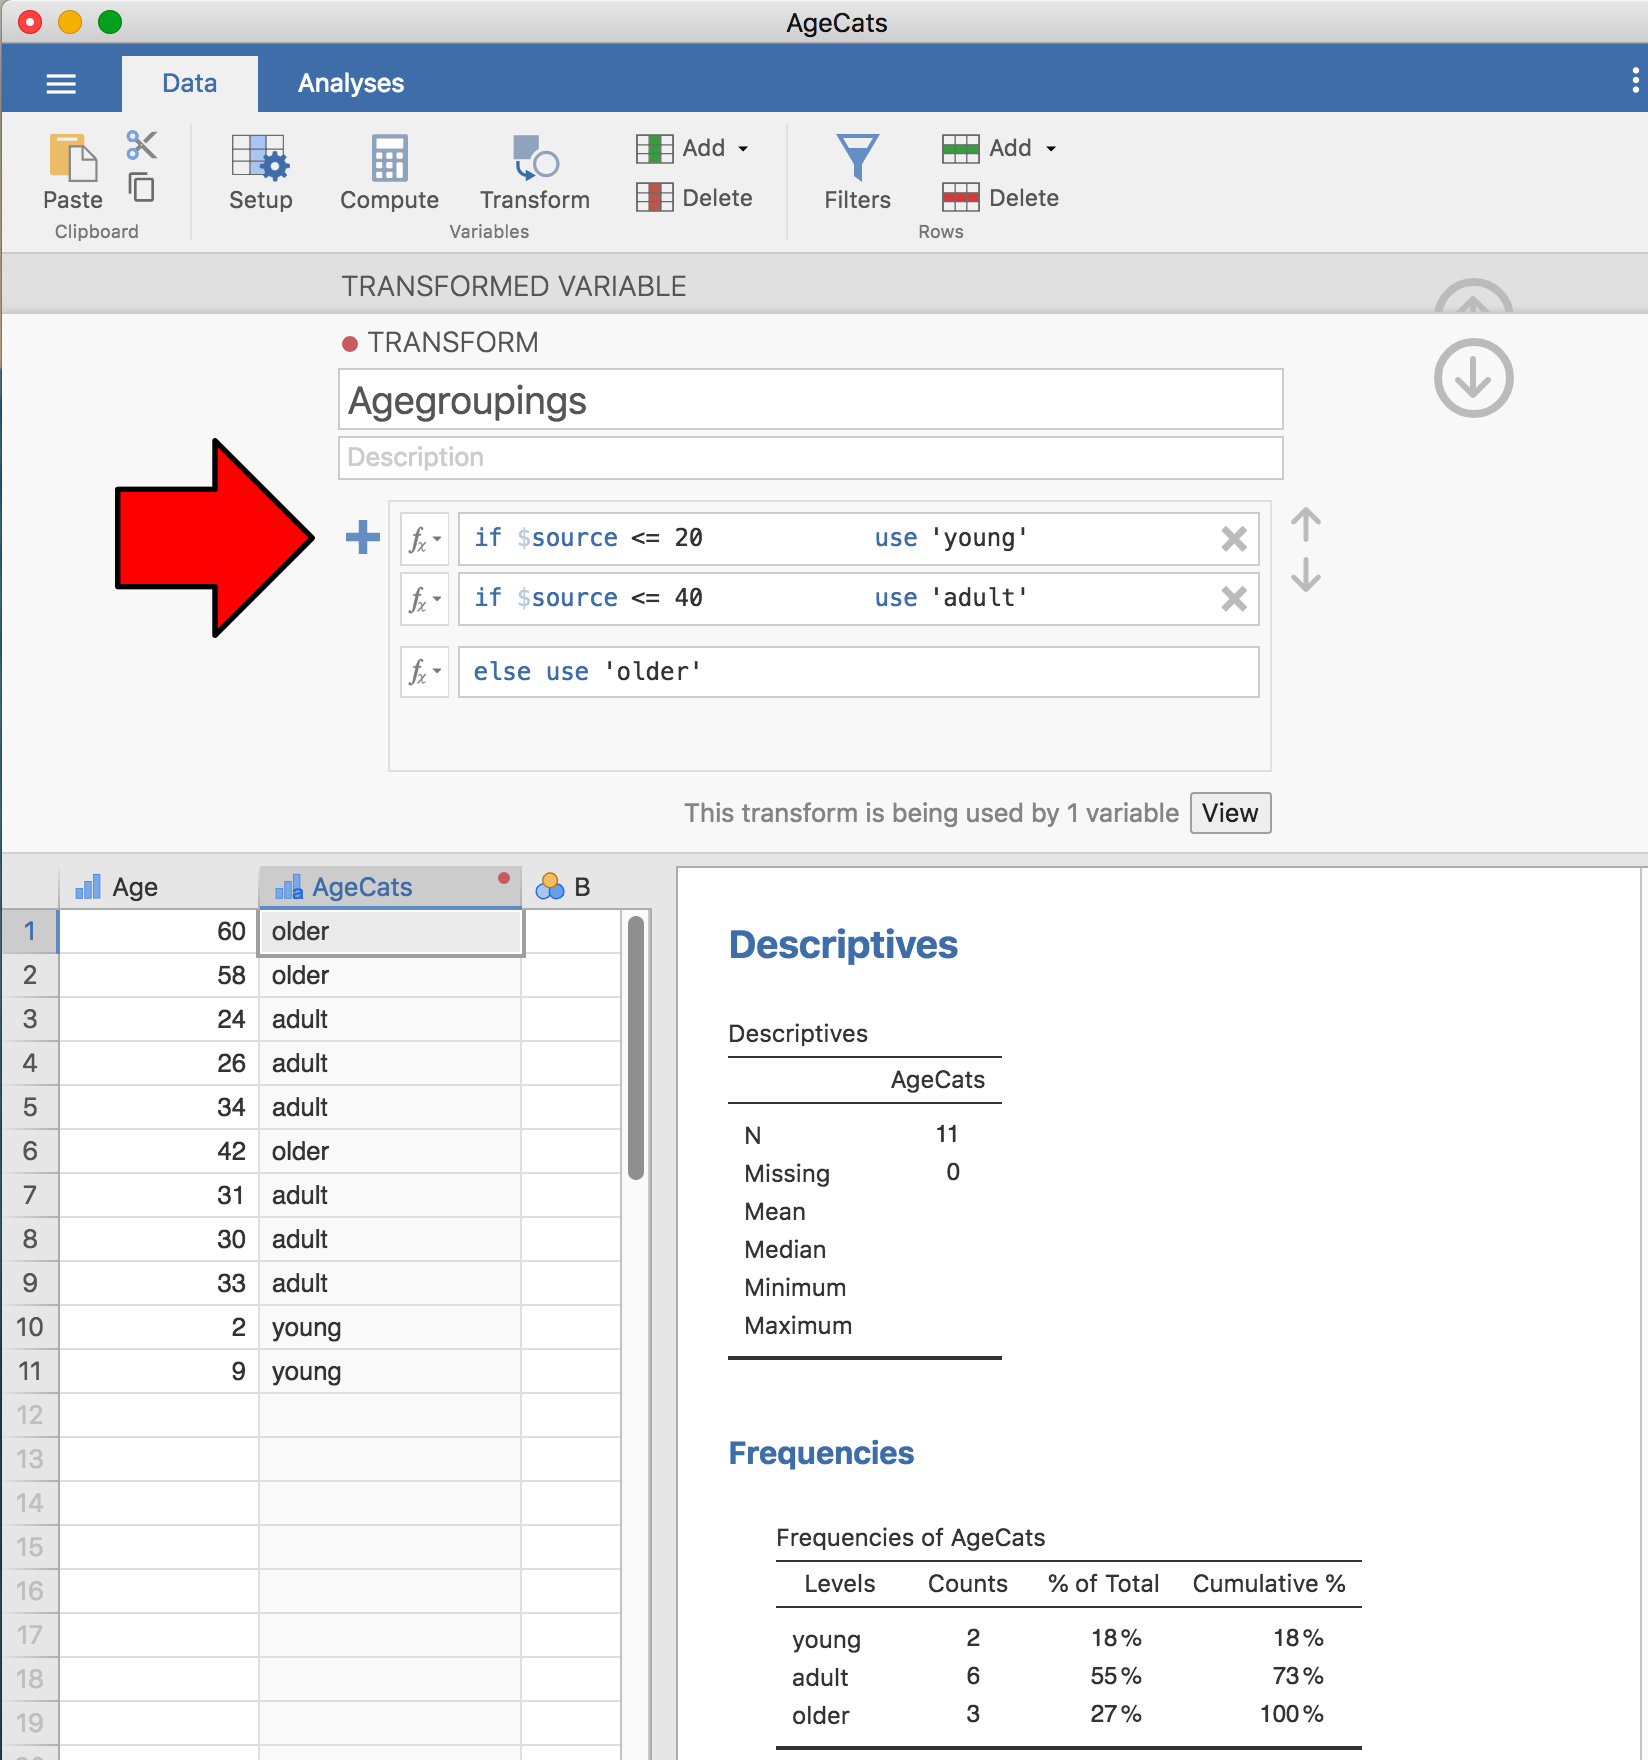
\includegraphics[width=1\linewidth]{img/mechanics/transform3} 

}

\caption{jamovi transformation into three age categories, using the 'Add condition' button}\label{fig:transform3}
\end{figure}

\hypertarget{mathfunc}{%
\section{A few more mathematical functions and operations}\label{mathfunc}}

In Section \ref{transform} I discussed the ideas behind variable transformations and showed that a lot of the transformations that you might want to apply to your data are based on fairly simple mathematical functions and operations. In this section I want to return to that discussion and mention several other mathematical functions and arithmetic operations that are actually quite useful for a lot of real world data analysis. Table \ref{tab:mathfunc} gives a brief overview of the various mathematical functions I want to talk about here, or later.\footnote{We'll leave the box-cox function until later on, see Subsection \ref{regressionnormality}} Obviously this doesn't even come close to cataloguing the range of possibilities available, but it does cover a range of functions that are used regularly in data analysis and that are available in jamovi.

\begin{table}

\caption{\label{tab:mathfunc}Some of the mathematical functions available in jamovi}
\centering
\begin{tabular}[t]{l|l|l|l}
\hline
mathematical.function & R.function & example.input & answer\\
\hline
square root & SQRT(x) & SQRT(25) & 5\\
\hline
absolute value & ABS(x) & ABS(-23) & 23\\
\hline
logarithm (base 10) & LOG10(x) & LOG10(1000) & 3\\
\hline
logarithm (base e) & LN(x) & LN(1000) & 6.908\\
\hline
exponentiation & EXP(x) & EXP(6.908) & 1000.245\\
\hline
box-cox & BOXCOX(x, lamda) & BOXCOX(6.908, 3) & 109.551\\
\hline
\end{tabular}
\end{table}

\hypertarget{logarithms-and-exponentials}{%
\subsection{Logarithms and exponentials}\label{logarithms-and-exponentials}}

As I've mentioned earlier, jamovi has an useful range of mathematical functions built into it and there really wouldn't be much point in trying to describe or even list all of them. For the most part, I've focused only on those functions that are strictly necessary for this book. However I do want to make an exception for logarithms and exponentials. Although they aren't needed anywhere else in this book, they are \emph{everywhere} in statistics more broadly. And not only that, there are a \emph{lot} of situations in which it is convenient to analyse the logarithm of a variable (i.e., to take a `log-transform' of the variable). I suspect that many (maybe most) readers of this book will have encountered logarithms and exponentials before, but from past experience I know that there's a substantial proportion of students who take a social science statistics class who haven't touched logarithms since high school, and would appreciate a bit of a refresher.

In order to understand logarithms and exponentials, the easiest thing to do is to actually calculate them and see how they relate to other simple calculations. There are three jamovi functions in particular that I want to talk about, namely \texttt{LN()}, \texttt{LOG10()} and \texttt{EXP()}. To start with, let's consider \texttt{LOG10()}, which is known as the `llogarithm in base 10.' The trick to understanding a {\textbf{logarithm}} is to understand that it's basically the ``opposite'' of taking a power. Specifically, the logarithm in base 10 is closely related to the powers of 10. So let's start by noting that 10-cubed is 1000. Mathematically, we would write this:
\[ 
10^3 = 1000
\]
The trick to understanding a logarithm is to recognise that the statement that ``10 to the power of 3 is equal to 1000'' is equivalent to the statement that ``the logarithm (in base 10) of 1000 is equal to 3.'' Mathematically, we write this as follows,
\[
\log_{10}( 1000 ) = 3
\]

Okay, since the \texttt{LOG10()} function is related to the powers of 10, you might expect that there are other logarithms (in bases other than 10) that are related to other powers too. And of course that's true: there's not really anything mathematically special about the number 10. You and I happen to find it useful because decimal numbers are built around the number 10, but the big bad world of mathematics scoffs at our decimal numbers. Sadly, the universe doesn't actually care how we write down numbers. Anyway, the consequence of this cosmic indifference is that there's nothing particularly special about calculating logarithms in base 10. You could, for instance, calculate your logarithms in base 2. Alternatively, a third type of logarithm, and one we see a lot more of in statistics than either base 10 or base 2, is called the {\textbf{natural logarithm}}, and corresponds to the logarithm in base \(e\). Since you might one day run into it, I'd better explain what \(e\) is. The number \(e\), known as {\textbf{Euler's number}}, is one of those annoying ``irrational'' numbers whose decimal expansion is infinitely long, and is considered one of the most important numbers in mathematics. The first few digits of \(e\) are:
\[
e = 2.718282 
\]
There are quite a few situation in statistics that require us to calculate powers of \(e\), though none of them appear in this book. Raising \(e\) to the power \(x\) is called the {\textbf{exponential}} of \(x\), and so it's very common to see \(e^x\) written as \(\exp(x)\). And so it's no surprise that jamovi has a function that calculates exponentials, called \texttt{EXP()}. Because the number \(e\) crops up so often in statistics, the natural logarithm (i.e., logarithm in base \(e\)) also tends to turn up. Mathematicians often write it as \(\log_e(x)\) or \(\ln(x)\). In fact, jamovi works the same way: the \texttt{LN()} function corresponds to the natural logarithm.

And with that, I think we've had quite enough exponentials and logarithms for this book!

\hypertarget{subset}{%
\section{Extracting a subset of the data}\label{subset}}

One very important kind of data handling is being able to extract a particular subset of the data. For instance, you might be interested only in analysing the data from one experimental condition, or you may want to look closely at the data from people over 50 years in age. To do this, the first step is getting jamovi to filter the subset of the data corresponding to the observations that you're interested in.

This section returns to the \textbf{\texttt{nightgarden.csv}} data set. If you're reading this whole chapter in one sitting, then you should already have this data set loaded into a jamovi window. For this section, let's focus on the two variables \textbf{\texttt{speaker}} and \textbf{\texttt{utterance}} (see Section \ref{freqtables} if you've forgotten what those variables look like). Suppose that what I want to do is pull out only those utterances that were made by Makka-Pakka. To that end, we need to specify a filter in jamovi. First open up a filter window by clicking on `Filters' on the main jamovi `Data' toolbar. Then, in the `Filter 1' text box, next to the `=' sign, type the following:

\texttt{speaker\ ==\ \textquotesingle{}makka-pakka\textquotesingle{}}

\begin{figure}

{\centering 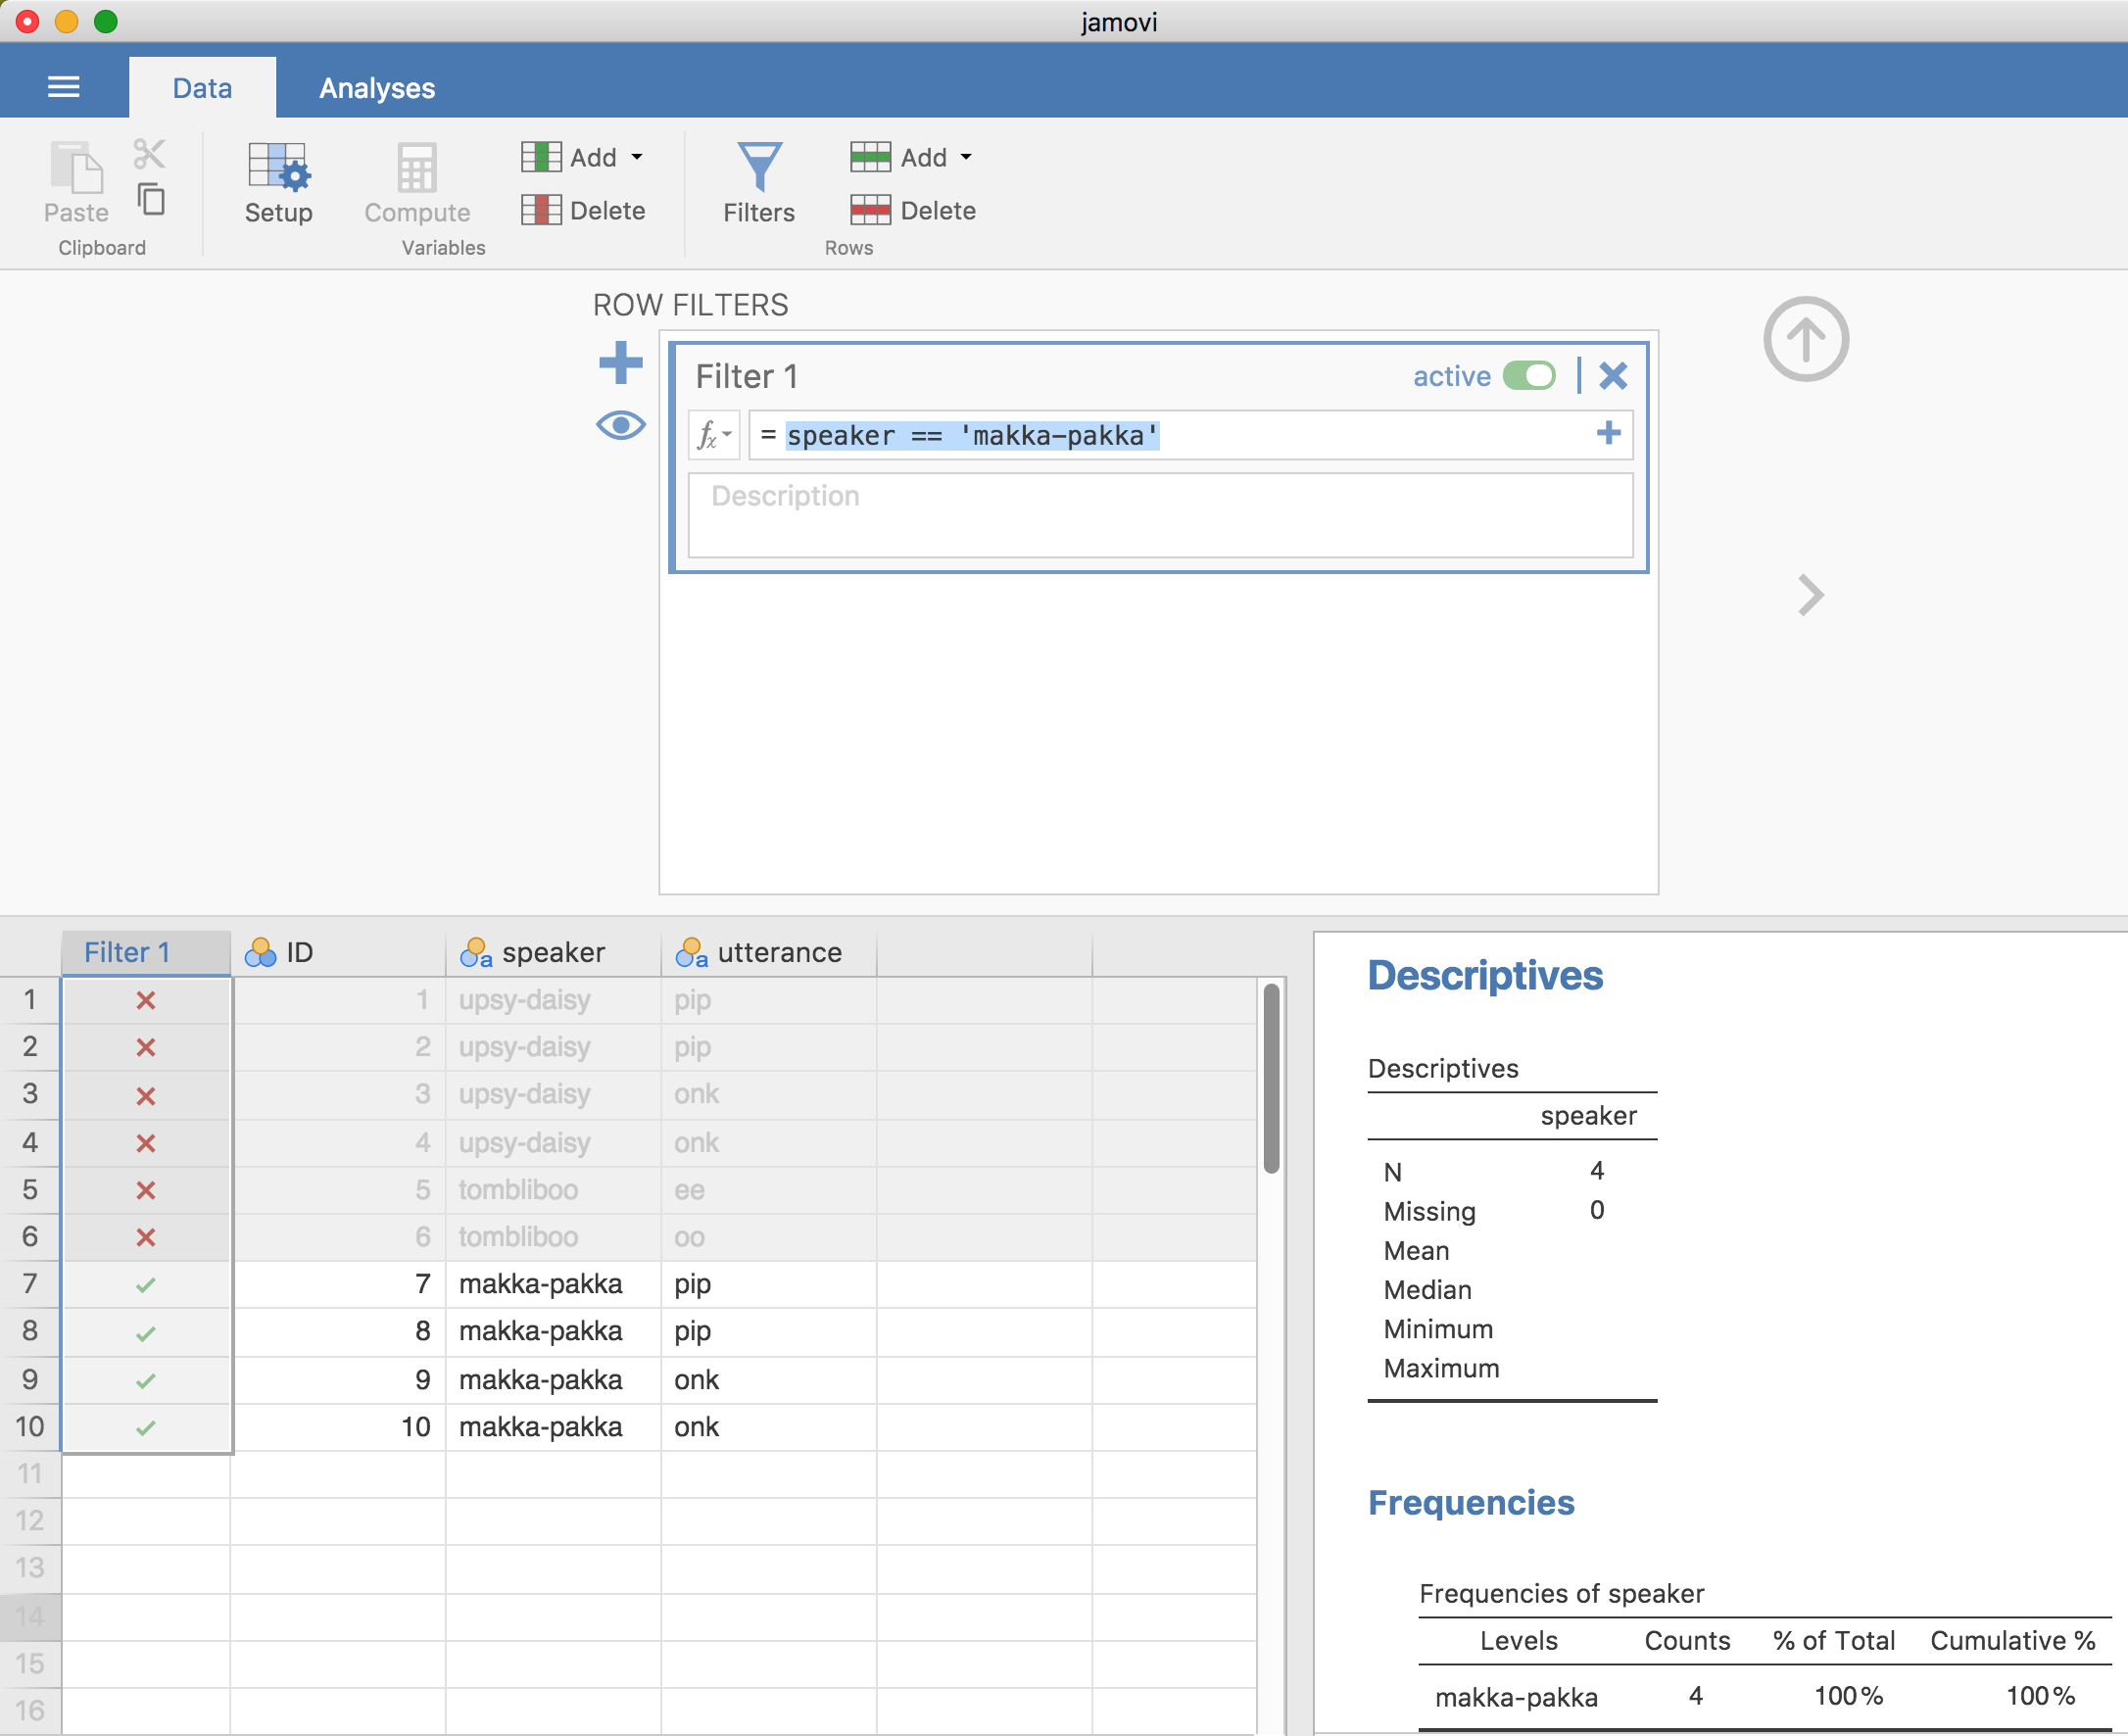
\includegraphics[width=1\linewidth]{img/mechanics/subset1} 

}

\caption{Creating a subset of the `nightgarden` data using the jamovi 'Filters' option}\label{fig:subset1}
\end{figure}

When you have done this, you will see that a new column has been added to the spreadsheet window (see Figure \ref{fig:subset1}), labelled `Filter 1,' with the cases where \textbf{\texttt{speaker}} \textbf{is not} `makka-pakka' greyed-out (i.e., filtered out) and, conversely, the cases where \textbf{\texttt{speaker}} \textbf{is} `makka-pakka' have a green check mark indicating they are filtered in. You can test this by running `Exploration' - `Descriptives' - `Frequency tables' for the \textbf{\texttt{speaker}} variable and seeing what that shows. Go on, try it!

Following on from this simple example, you can also build up more complex filters using logical expressions in jamovi. For instance, suppose I wanted to keep only those cases when the utterance is either `pip' or `oo.' In this case in the `Filter 1' text box, next to the `=' sign, you would type the following:

\texttt{utterance\ ==\ \textquotesingle{}pip\textquotesingle{}\ or\ utterance\ ==\ \textquotesingle{}oo\textquotesingle{}}

\hypertarget{summary-3}{%
\section{Summary}\label{summary-3}}

Obviously, there's no real coherence to this chapter. It's just a grab bag of topics and tricks that can be handy to know about, so the best wrap up I can give here is just to repeat this list:

\begin{itemize}
\tightlist
\item
  Section \ref{freqtables}. Tabulating data.
\item
  Section \ref{logicals}. Using logical expressions.
\item
  Section \ref{transform}. Transforming or recoding a variable.
\item
  Section \ref{mathfunc}. Some useful mathematical functions.
\item
  Section \ref{subset}. Extracting a subset of a data set.
\end{itemize}

\hypertarget{part-iv.-statistical-theory}{%
\chapter*{Part IV. Statistical Theory}\label{part-iv.-statistical-theory}}
\addcontentsline{toc}{chapter}{Part IV. Statistical Theory}

\hypertarget{prelude-to-part-iv}{%
\chapter*{Prelude to Part IV}\label{prelude-to-part-iv}}
\addcontentsline{toc}{chapter}{Prelude to Part IV}

Part IV of the book is by far the most theoretical, focusing as it does on the theory of statistical inference. Over the next three chapters my goal is to give you an introduction to probability theory (Chapter \ref{probability}), sampling and estimation (Chapter \ref{estimation}) and statistical hypothesis testing (Chapter \ref{hypothesistesting}). Before we get started though, I want to say something about the big picture. Statistical inference is primarily about \emph{learning from data} The goal is no longer merely to describe our data but to use the data to draw conclusions about the world. To motivate the discussion I want to spend a bit of time talking about a philosophical puzzle known as the \emph{riddle of induction}, because it speaks to an issue that will pop up over and over again throughout the book: statistical inference relies on \emph{assumptions}. This sounds like a bad thing. In everyday life people say things like ``you should never make assumptions,'' and psychology classes often talk about assumptions and biases as bad things that we should try to avoid. From bitter personal experience I have learned never to say such things around philosophers!

\hypertarget{on-the-limits-of-logical-reasoning}{%
\section*{On the limits of logical reasoning}\label{on-the-limits-of-logical-reasoning}}
\addcontentsline{toc}{section}{On the limits of logical reasoning}

~~~~~~\emph{The whole art of war consists in getting at what is on the other side of the hill, or, in other words, in learning what we do not know from what we do.}\\
\hspace*{0.333em}\hspace*{0.333em}\hspace*{0.333em}\hspace*{0.333em}\hspace*{0.333em}\hspace*{0.333em}\hspace*{0.333em}\hspace*{0.333em}\hspace*{0.333em}\hspace*{0.333em}\hspace*{0.333em}\hspace*{0.333em}\hspace*{0.333em}\hspace*{0.333em}\hspace*{0.333em}\hspace*{0.333em}\hspace*{0.333em}\hspace*{0.333em}\hspace*{0.333em}\hspace*{0.333em}\hspace*{0.333em}\hspace*{0.333em}\hspace*{0.333em}\hspace*{0.333em}\hspace*{0.333em}\hspace*{0.333em}\hspace*{0.333em}\hspace*{0.333em}\hspace*{0.333em}\hspace*{0.333em}-- Arthur Wellesley, 1st Duke of Wellington

I am told that quote above came about as a consequence of a carriage ride across the countryside.\footnote{\url{http://www.bartleby.com/344/400.html}} He and his companion, J. W. Croker, were playing a guessing game, each trying to predict what would be on the other side of each hill. In every case it turned out that Wellesley was right and Croker was wrong. Many years later when Wellesley was asked about the game he explained that ``the whole art of war consists in getting at what is on the other side of the hill.'' Indeed, war is not special in this respect. All of life is a guessing game of one form or another, and getting by on a day to day basis requires us to make good guesses. So let's play a guessing game of our own.

Suppose you and I are observing the Wellesley-Croker competition and after every three hills you and I have to predict who will win the next one, Wellesley or Croker. Let's say that ``W'' refers to a Wellesley victory and ``C'' refers to a Croker victory. After three hills, our data set looks like this:

\begin{verbatim}
WWW
\end{verbatim}

Our conversation goes like this:
- YOU: Three in a row doesn't mean much. I suppose Wellesley might be better at this than Croker, but it might just be luck. Still, I'm a bit of a gambler. I'll bet on Wellesley.
- ME: I agree that three in a row isn't informative and I see no reason to prefer Wellesley's guesses over Croker's. I can't justify betting at this stage. Sorry. No bet for me.

Your gamble paid off: three more hills go by and Wellesley wins all three. Going into the next round of our game the score is 1-0 in favour of you and our data set looks like this:

\begin{verbatim}
WWW WWW
\end{verbatim}

I've organised the data into blocks of three so that you can see which batch corresponds to the observations that we had available at each step in our little side game. After seeing this new batch, our conversation continues:

\begin{itemize}
\tightlist
\item
  YOU: Six wins in a row for Duke Wellesley. This is starting to feel a bit suspicious. I'm still not certain, but I reckon that he's going to win the next one too.
\item
  ME: I guess I don't see that. Sure, I agree that Wellesley has won six in a row, but I don't see any logical reason why that means he'll win the seventh one. No bet.
\item
  YOU: Do you really think so? Fair enough, but my bet worked out last time and I'm okay with my choice.
\end{itemize}

For a second time you were right, and for a second time I was wrong. Wellesley wins the next three hills, extending his winning record against Croker to 9-0. The data set available to us is now this:

\begin{verbatim}
WWW WWW WWW
\end{verbatim}

And our conversation goes like this:

\begin{itemize}
\tightlist
\item
  YOU: Okay, this is pretty obvious. Wellesley is way better at this game. We both agree he's going to win the next hill, right?
\item
  ME: Is there really any logical evidence for that? Before we started this game, there were lots of possibilities for the first 10 outcomes, and I had no idea which one to expect. ``WWW WWW WWW W'' was one possibility, but so was ``\{WCC CWC WWC C'' and ``WWW WWW WWW C'' or even ``\{CCC CCC CCC C.'' Because I had no idea what would happen so I'd have said they were all equally likely. I assume you would have too, right? I mean, that's what it \emph{means} to say you have ``no idea,'' isn't it?
\item
  YOU: I suppose so.
\item
  ME: Well then, the observations we've made logically rule out all possibilities except two: ``WWW WWW WWW C'' or ``WWW WWW WWW W.'' Both of these are perfectly consistent with the evidence we've encountered so far, aren't they?\\
\item
  YOU: Yes, of course they are. Where are you going with this?
\item
  ME: So what's changed then? At the start of our game, you'd have agreed with me that these are equally plausible and none of the evidence that we've encountered has discriminated between these two possibilities. Therefore, both of these possibilities remain equally plausible and I see no logical reason to prefer one over the other. So yes, while I agree with you that Wellesley's run of 9 wins in a row is remarkable, I can't think of a good reason to think he'll win the 10th hill. No bet.
\item
  YOU: I see your point, but I'm still willing to chance it. I'm betting on Wellesley.
\end{itemize}

Wellesley's winning streak continues for the next three hills. The score in the Wellesley-Croker game is now 12-0, and the score in our game is now 3-0. As we approach the fourth round of our game, our data set is this:

\begin{verbatim}
WWW WWW WWW WWW
\end{verbatim}

and the conversation continues:

\begin{itemize}
\tightlist
\item
  YOU: Oh yeah! Three more wins for Wellesley and another victory for me. Admit it, I was right about him! I guess we're both betting on Wellesley this time around, right?
\item
  ME: I don't know what to think. I feel like we're in the same situation we were in last round, and nothing much has changed. There are only two legitimate possibilities for a sequence of 13 hills that haven't already been ruled out, ``WWW WWW WWW WWW C'' and ``WWW WWW WWW WWW W.'' It's just like I said last time. If all possible outcomes were equally sensible before the game started, shouldn't these two be equally sensible now given that our observations don't rule out either one? I agree that it feels like Wellesley is on an amazing winning streak, but where's the logical evidence that the streak will continue?
\item
  YOU: I think you're being unreasonable. Why not take a look at \emph{our} scorecard, if you need evidence? You're the expert on statistics and you've been using this fancy logical analysis, but the fact is you're losing. I'm just relying on common sense and I'm winning. Maybe you should switch strategies.
\item
  ME: Hmm, that is a good point and I don't want to lose the game, but I'm afraid I don't see any logical evidence that your strategy is better than mine. It seems to me that if there were someone else watching our game, what they'd have observed is a run of three wins to you. Their data would look like this: ``YYY.'' Logically, I don't see that this is any different to our first round of watching Wellesley and Croker. Three wins to you doesn't seem like a lot of evidence, and I see no reason to think that your strategy is working out any better than mine. If I didn't think that ``WWW'' was good evidence then for Wellesley being better than Croker at \emph{their} game, surely I have no reason now to think that ``YYY'' is good evidence that you're better at \emph{ours}?
\item
  YOU: Okay, now I think you're being a jerk.
\item
  ME: I don't see the logical evidence for that.
\end{itemize}

\hypertarget{learning-without-making-assumptions-is-a-myth}{%
\section*{Learning without making assumptions is a myth}\label{learning-without-making-assumptions-is-a-myth}}
\addcontentsline{toc}{section}{Learning without making assumptions is a myth}

There are lots of different ways in which we could dissect this dialogue, but since this is a statistics book pitched at psychologists and not an introduction to the philosophy and psychology of reasoning, I'll keep it brief. What I've described above is sometimes referred to as the riddle of induction. It seems entirely \emph{reasonable} to think that a 12-0 winning record by Wellesley is pretty strong evidence that he will win the 13th game, but it is not easy to provide a proper logical justification for this belief. On the contrary, despite the \emph{obviousness} of the answer, it's not actually possible to justify betting on Wellesley without relying on some assumption that you don't have any logical justification for.

The riddle of induction is most associated with the philosophical work of David Hume and more recently Nelson Goodman, but you can find examples of the problem popping up in fields as diverse as literature (Lewis Carroll) and machine learning (the ``no free lunch'' theorem). There really is something weird about trying to ``learn what we do not know from what we do know.'' The critical point is that assumptions and biases are unavoidable if you want to learn anything about the world. There is no escape from this, and it is just as true for statistical inference as it is for human reasoning. In the dialogue I was taking aim at your perfectly sensible inferences as a human being, but the common sense reasoning that you relied on is no different to what a statistician would have done. Your ``common sense'' half of the dialog relied on an implicit \emph{assumption} that there exists some difference in skill between Wellesley and Croker, and what you were doing was trying to work out what that difference in skill level would be. My ``logical analysis'' rejects that assumption entirely. All I was willing to accept is that there are sequences of wins and losses and that I did not know which sequences would be observed. Throughout the dialogue I kept insisting that all logically possible data sets were equally plausible at the start of the Wellesely-Croker game, and the only way in which I ever revised my beliefs was to eliminate those possibilities that were factually inconsistent with the observations.

That sounds perfectly sensible on its own terms. In fact, it even sounds like the hallmark of good deductive reasoning. Like Sherlock Holmes, my approach was to rule out that which is impossible in the hope that what would be left is the truth. Yet as we saw, ruling out the impossible \emph{never} led me to make a prediction. On its own terms everything I said in my half of the dialogue was entirely correct. An inability to make any predictions is the logical consequence of making ``no assumptions.'' In the end I lost our game because you did make some assumptions and those assumptions turned out to be right. Skill is a real thing, and because you believed in the existence of skill you were able to learn that Wellesley had more of it than Croker. Had you relied on a less sensible assumption to drive your learning you might not have won the game.

Ultimately there are two things you should take away from this. First, as I've said, you cannot avoid making assumptions if you want to learn anything from your data. But second, once you realise that assumptions are necessary it becomes important to make sure you \emph{make the right ones!} A data analysis that relies on few assumptions is not necessarily better than one that makes many assumptions, it all depends on whether those assumptions are good ones for your data. As we go through the rest of this book I'll often point out the assumptions that underpin a particular statistical technique, and how you can check whether those assumptions are sensible.

\hypertarget{hypothesistesting}{%
\chapter{Hypothesis testing}\label{hypothesistesting}}

~~~~~~\emph{The process of induction is the process of assuming the simplest law that can be made to harmonize with our experience. This process, however, has no logical foundation but only a psychological one. It is clear that there are no grounds for believing that the simplest course of events will really happen. It is an hypothesis that the sun will rise tomorrow: and this means that we do not know whether it will rise.}\\
\hspace*{0.333em}\hspace*{0.333em}\hspace*{0.333em}\hspace*{0.333em}\hspace*{0.333em}\hspace*{0.333em}\hspace*{0.333em}\hspace*{0.333em}\hspace*{0.333em}\hspace*{0.333em}\hspace*{0.333em}\hspace*{0.333em}\hspace*{0.333em}\hspace*{0.333em}\hspace*{0.333em}\hspace*{0.333em}\hspace*{0.333em}\hspace*{0.333em}\hspace*{0.333em}\hspace*{0.333em}\hspace*{0.333em}\hspace*{0.333em}\hspace*{0.333em}\hspace*{0.333em}\hspace*{0.333em}\hspace*{0.333em}\hspace*{0.333em}\hspace*{0.333em}\hspace*{0.333em}\hspace*{0.333em}-- Ludwig Wittgenstein\footnote{The quote comes from Wittgenstein's (1922) text, \emph{Tractatus Logico-Philosphicus}.}

In the last chapter I discussed the ideas behind estimation, which is one of the two ``big ideas'' in inferential statistics. It's now time to turn our attention to the other big idea, which is \emph{hypothesis testing}. In its most abstract form, hypothesis testing is really a very simple idea. The researcher has some theory about the world and wants to determine whether or not the data actually support that theory. However, the details are messy and most people find the theory of hypothesis testing to be the most frustrating part of statistics. The structure of the chapter is as follows. First, I'll describe how hypothesis testing works in a fair amount of detail, using a simple running example to show you how a hypothesis test is ``built.'' I'll try to avoid being too dogmatic while doing so, and focus instead on the underlying logic of the testing procedure.\footnote{A technical note. The description below differs subtly from the standard description given in a lot of introductory texts. The orthodox theory of null hypothesis testing emerged from the work of Sir Ronald Fisher and Jerzy Neyman in the early 20th century; but Fisher and Neyman actually had very different views about how it should work. The standard treatment of hypothesis testing that most texts use is a hybrid of the two approaches. The treatment here is a little more Neyman-style than the orthodox view, especially as regards the meaning of the \(p\) value.} Afterwards, I'll spend a bit of time talking about the various dogmas, rules and heresies that surround the theory of hypothesis testing.

\hypertarget{hypotheses}{%
\section{A menagerie of hypotheses}\label{hypotheses}}

Eventually we all succumb to madness. For me, that day will arrive once I'm finally promoted to full professor. Safely ensconced in my ivory tower, happily protected by tenure, I will finally be able to take leave of my senses (so to speak) and indulge in that most thoroughly unproductive line of psychological research, the search for extrasensory perception (ESP).\footnote{My apologies to anyone who actually believes in this stuff, but on my reading of the literature on ESP it's just not reasonable to think this is real. To be fair, though, some of the studies are rigorously designed, so it's actually an interesting area for thinking about psychological research design. And of course it's a free country so you can spend your own time and effort proving me wrong if you like, but I wouldn't think that's a terribly practical use of your intellect.}

Let's suppose that this glorious day has come. My first study is a simple one in which I seek to test whether clairvoyance exists. Each participant sits down at a table and is shown a card by an experimenter. The card is black on one side and white on the other. The experimenter takes the card away and places it on a table in an adjacent room. The card is placed black side up or white side up completely at random, with the randomisation occurring only after the experimenter has left the room with the participant. A second experimenter comes in and asks the participant which side of the card is now facing upwards. It's purely a one-shot experiment. Each person sees only one card and gives only one answer, and at no stage is the participant actually in contact with someone who knows the right answer. My data set, therefore, is very simple. I have asked the question of \(N\) people and some number \(X\) of these people have given the correct response. To make things concrete, let's suppose that I have tested \(N = 100\) people and \(X = 62\) of these got the answer right. A surprisingly large number, sure, but is it large enough for me to feel safe in claiming I've found evidence for ESP? This is the situation where hypothesis testing comes in useful. However, before we talk about how to \emph{test} hypotheses, we need to be clear about what we mean by hypotheses.

\hypertarget{research-hypotheses-versus-statistical-hypotheses}{%
\subsection{Research hypotheses versus statistical hypotheses}\label{research-hypotheses-versus-statistical-hypotheses}}

The first distinction that you need to keep clear in your mind is between research hypotheses and statistical hypotheses. In my ESP study my overall scientific goal is to demonstrate that clairvoyance exists. In this situation I have a clear research goal: I am hoping to discover evidence for ESP. In other situations I might actually be a lot more neutral than that, so I might say that my research goal is to determine whether or not clairvoyance exists. Regardless of how I want to portray myself, the basic point that I'm trying to convey here is that a research hypothesis involves making a substantive, testable scientific claim. If you are a psychologist then your research hypotheses are fundamentally \emph{about} psychological constructs. Any of the following would count as {\textbf{research hypotheses}}:

\begin{itemize}
\tightlist
\item
  \emph{Listening to music reduces your ability to pay attention to other things.} This is a claim about the causal relationship between two psychologically meaningful concepts (listening to music and paying attention to things), so it's a perfectly reasonable research hypothesis.
\item
  \emph{Intelligence is related to personality}. Like the last one, this is a relational claim about two psychological constructs (intelligence and personality), but the claim is weaker: correlational not causal.
\item
  \emph{Intelligence} \textbf{\emph{is}} \emph{speed of information processing}. This hypothesis has a quite different character. It's not actually a relational claim at all. It's an ontological claim about the fundamental character of intelligence (and I'm pretty sure it's wrong). It's worth expanding on this one actually. It's usually easier to think about how to construct experiments to test research hypotheses of the form ``does X affect Y?'' than it is to address claims like ``what is X?'' And in practice what usually happens is that you find ways of testing relational claims that follow from your ontological ones. For instance, if I believe that intelligence \emph{is} speed of information processing in the brain, my experiments will often involve looking for relationships between measures of intelligence and measures of speed. As a consequence most everyday research questions do tend to be relational in nature, but they're almost always motivated by deeper ontological questions about the state of nature.
\end{itemize}

Notice that in practice, my research hypotheses could overlap a lot. My ultimate goal in the ESP experiment might be to test an ontological claim like ``ESP exists,'' but I might operationally restrict myself to a narrower hypothesis like ``Some people can `see' objects in a clairvoyant fashion.'' That said, there are some things that really don't count as proper research hypotheses in any meaningful sense:

\begin{itemize}
\tightlist
\item
  \emph{Love is a battlefield}. This is too vague to be testable. Whilst it's okay for a research hypothesis to have a degree of vagueness to it, it has to be possible to operationalise your theoretical ideas. Maybe I'm just not creative enough to see it, but I can't see how this can be converted into any concrete research design. If that's true then this isn't a scientific research hypothesis, it's a pop song. That doesn't mean it's not interesting. A lot of deep questions that humans have fall into this category. Maybe one day science will be able to construct testable theories of love, or to test to see if God exists, and so on. But right now we can't, and I wouldn't bet on ever seeing a satisfying scientific approach to either.
\item
  \emph{The first rule of tautology club is the first rule of tautology club}. This is not a substantive claim of any kind. It's true by definition. No conceivable state of nature could possibly be inconsistent with this claim. We say that this is an unfalsifiable hypothesis, and as such it is outside the domain of science. Whatever else you do in science your claims must have the possibility of being wrong.
\item
  \emph{More people in my experiment will say ``yes'' than ``no''}. This one fails as a research hypothesis because it's a claim about the data set, not about the psychology (unless of course your actual research question is whether people have some kind of ``yes'' bias!). Actually, this hypothesis is starting to sound more like a statistical hypothesis than a research hypothesis.
\end{itemize}

As you can see, research hypotheses can be somewhat messy at times and ultimately they are \emph{scientific} claims. {\textbf{Statistical hypotheses}} are neither of these two things. Statistical hypotheses must be mathematically precise and they must correspond to specific claims about the characteristics of the data generating mechanism (i.e., the ``population''). Even so, the intent is that statistical hypotheses bear a clear relationship to the substantive research hypotheses that you care about! For instance, in my ESP study my research hypothesis is that some people are able to see through walls or whatever. What I want to do is to ``map'' this onto a statement about how the data were generated. So let's think about what that statement would be. The quantity that I'm interested in within the experiment is \(P(\mbox{"correct"})\), the true-but-unknown probability with which the participants in my experiment answer the question correctly. Let's use the Greek letter \(\theta\) (theta) to refer to this probability. Here are four different statistical hypotheses:

\begin{itemize}
\tightlist
\item
  If ESP doesn't exist and if my experiment is well designed then my participants are just guessing. So I should expect them to get it right half of the time and so my statistical hypothesis is that the true probability of choosing correctly is \(\theta = 0.5\).
\item
  Alternatively, suppose ESP does exist and participants can see the card. If that's true people will perform better than chance and the statistical hypothesis is that \(\theta > 0.5\).
\item
  A third possibility is that ESP does exist, but the colours are all reversed and people don't realise it (okay, that's wacky, but you never know). If that's how it works then you'd expect people's performance to be \emph{below} chance. This would correspond to a statistical hypothesis that \(\theta < 0.5\).
\item
  Finally, suppose ESP exists but I have no idea whether people are seeing the right colour or the wrong one. In that case the only claim I could make about the data would be that the probability of making the correct answer is \emph{not} equal to 0.5. This corresponds to the statistical hypothesis that \(\theta \neq 0.5\).
\end{itemize}

All of these are legitimate examples of a statistical hypothesis because they are statements about a population parameter and are meaningfully related to my experiment.

What this discussion makes clear, I hope, is that when attempting to construct a statistical hypothesis test the researcher actually has two quite distinct hypotheses to consider. First, he or she has a research hypothesis (a claim about psychology), and this then corresponds to a statistical hypothesis (a claim about the data generating population). In my ESP example these might be:

\[
\begin{array}{cc}
\mbox{Dani's research hypothesis: } ``\mbox{ESP exists}" \\
\mbox{Dani's statistical hypothesis: } \theta \neq 0.5 \\
\end{array}
\]
And a key thing to recognise is this. \emph{A statistical hypothesis test is a test of the statistical hypothesis, not the research hypothesis}. If your study is badly designed then the link between your research hypothesis and your statistical hypothesis is broken. To give a silly example, suppose that my ESP study was conducted in a situation where the participant can actually see the card reflected in a window. If that happens I would be able to find very strong evidence that \(\theta \neq 0.5\), but this would tell us nothing about whether ``ESP exists.''

\hypertarget{null-hypotheses-and-alternative-hypotheses}{%
\subsection{Null hypotheses and alternative hypotheses}\label{null-hypotheses-and-alternative-hypotheses}}

So far, so good. I have a research hypothesis that corresponds to what I want to believe about the world, and I can map it onto a statistical hypothesis that corresponds to what I want to believe about how the data were generated. It's at this point that things get somewhat counter-intuitive for a lot of people. Because what I'm about to do is invent a new statistical hypothesis (the ``null'' hypothesis, \(H_0\)) that corresponds to the exact opposite of what I want to believe, and then focus exclusively on that almost to the neglect of the thing I'm actually interested in (which is now called the ``alternative'' hypothesis, \(H_1\)). In our ESP example, the null hypothesis is that \(\theta = 0.5\), since that's what we'd expect if ESP \emph{didn't} exist. My hope, of course, is that ESP is totally real and so the \emph{alternative} to this null hypothesis is \(\theta \neq 0.5\). In essence, what we're doing here is dividing up the possible values of \(\theta\) into two groups: those values that I really hope aren't true (the null), and those values that I'd be happy with if they turn out to be right (the alternative). Having done so, the important thing to recognise is that the goal of a hypothesis test is \emph{not} to show that the alternative hypothesis is (probably) true. The goal is to show that the null hypothesis is (probably) false. Most people find this pretty weird.

The best way to think about it, in my experience, is to imagine that a hypothesis test is a criminal trial\footnote{This analogy only works if you're from an adversarial legal system like UK/US/Australia. As I understand these things, the French inquisitorial system is quite different.}, \emph{the trial of the null hypothesis}. The null hypothesis is the defendant, the researcher is the prosecutor, and the statistical test itself is the judge. Just like a criminal trial, there is a presumption of innocence. The null hypothesis is \emph{deemed} to be true unless you, the researcher, can prove beyond a reasonable doubt that it is false. You are free to design your experiment however you like (within reason, obviously!) and your goal when doing so is to maximise the chance that the data will yield a conviction for the crime of being false. The catch is that the statistical test sets the rules of the trial and those rules are designed to protect the null hypothesis, specifically to ensure that if the null hypothesis is actually true the chances of a false conviction are guaranteed to be low. This is pretty important. After all, the null hypothesis doesn't get a lawyer, and given that the researcher is trying desperately to prove it to be false \emph{someone} has to protect it.

\hypertarget{errortypes}{%
\section{Two types of errors}\label{errortypes}}

Before going into details about how a statistical test is constructed it's useful to understand the philosophy behind it. I hinted at it when pointing out the similarity between a null hypothesis test and a criminal trial, but I should now be explicit. Ideally, we would like to construct our test so that we never make any errors. Unfortunately, since the world is messy, this is never possible. Sometimes you're just really unlucky. For instance, suppose you flip a coin 10 times in a row and it comes up heads all 10 times. That feels like very strong evidence for a conclusion that the coin is biased, but of course there's a 1 in 1024 chance that this would happen even if the coin was totally fair. In other words, in real life we \emph{always} have to accept that there's a chance that we made a mistake. As a consequence the goal behind statistical hypothesis testing is not to \emph{eliminate} errors, but to \emph{minimise} them.

At this point, we need to be a bit more precise about what we mean by ``errors.'' First, let's state the obvious. It is either the case that the null hypothesis is true or that it is false, and our test will either retain the null hypothesis or reject it.\footnote{An aside regarding the language you use to talk about hypothesis testing. First, one thing you really want to avoid is the word ``prove.'' A statistical test really doesn't \emph{prove} that a hypothesis is true or false. Proof implies certainty and, as the saying goes, statistics means never having to say you're certain. On that point almost everyone would agree. However, beyond that there's a fair amount of confusion. Some people argue that you're only allowed to make statements like ``rejected the null,'' ``failed to reject the null,'' or possibly ``retained the null.'' According to this line of thinking you can't say things like ``accept the alternative'' or ``accept the null.'' Personally I think this is too strong. In my opinion, this conflates null hypothesis testing with Karl Popper's falsificationist view of the scientific process. Whilst there are similarities between falsificationism and null hypothesis testing, they aren't equivalent. However, whilst I personally think it's fine to talk about accepting a hypothesis (on the proviso that ``acceptance'' doesn't actually mean that it's necessarily true, especially in the case of the null hypothesis), many people will disagree. And more to the point, you should be aware that this particular weirdness exists so that you're not caught unawares by it when writing up your own results.} So, as the table below illustrates, after we run the test and make our choice one of four things might have happened:

\begin{tabular}{l|c|c}
\hline
 & retain \$H\_0\$ & reject \$H\_0\$\\
\hline
\$H\_0\$ is true & correct decision & error (type I)\\
\hline
\$H\_0\$ is false & error (type II) & correct decision\\
\hline
\end{tabular}

As a consequence there are actually \emph{two} different types of error here. If we reject a null hypothesis that is actually true then we have made a {\textbf{type I error}}. On the other hand, if we retain the null hypothesis when it is in fact false then we have made a {\textbf{type II error}}.

Remember how I said that statistical testing was kind of like a criminal trial? Well, I meant it. A criminal trial requires that you establish ``beyond a reasonable doubt'' that the defendant did it. All of the evidential rules are (in theory, at least) designed to ensure that there's (almost) no chance of wrongfully convicting an innocent defendant. The trial is designed to protect the rights of a defendant, as the English jurist William Blackstone famously said, it is ``better that ten guilty persons escape than that one innocent suffer.'' In other words, a criminal trial doesn't treat the two types of error in the same way. Punishing the innocent is deemed to be much worse than letting the guilty go free. A statistical test is pretty much the same. The single most important design principle of the test is to \emph{control} the probability of a type I error, to keep it below some fixed probability. This probability, which is denoted \(\alpha\), is called the {\textbf{significance level}} of the test. And I'll say it again, because it is so central to the whole set-up, a hypothesis test is said to have significance level \(\alpha\) if the type I error rate is no larger than \(\alpha\).

So, what about the type II error rate? Well, we'd also like to keep those under control too, and we denote this probability by \(\beta\). However, it's much more common to refer to the {\textbf{power}} of the test, that is the probability with which we reject a null hypothesis when it really is false, which is \(1-\beta\). To help keep this straight, here's the same table again but with the relevant numbers added:

\begin{tabular}{l|c|c}
\hline
 & retain \$H\_0\$ & reject \$H\_0\$\\
\hline
\$H\_0\$ is true & \$1-\textbackslash{}alpha\$ (probability of correct retention) & \$\textbackslash{}alpha\$ (type I error rate)\\
\hline
\$H\_0\$ is false & \$\textbackslash{}beta\$ (type II error rate) & \$1-\textbackslash{}beta\$  (power of the test)\\
\hline
\end{tabular}

A ``powerful'' hypothesis test is one that has a small value of \(\beta\), while still keeping \(\alpha\) fixed at some (small) desired level. By convention, scientists make use of three different \(\alpha\) levels: \(.05\), \(.01\) and \(.001\). Notice the asymmetry here; the tests are designed to \emph{ensure} that the \(\alpha\) level is kept small but there's no corresponding guarantee regarding \(\beta\). We'd certainly \emph{like} the type II error rate to be small and we try to design tests that keep it small, but this is typically secondary to the overwhelming need to control the type I error rate. As Blackstone might have said if he were a statistician, it is ``better to retain 10 false null hypotheses than to reject a single true one.'' To be honest, I don't know that I agree with this philosophy. There are situations where I think it makes sense, and situations where I think it doesn't, but that's neither here nor there. It's how the tests are built.

\hypertarget{teststatistics}{%
\section{Test statistics and sampling distributions}\label{teststatistics}}

At this point we need to start talking specifics about how a hypothesis test is constructed. To that end, let's return to the ESP example. Let's ignore the actual data that we obtained, for the moment, and think about the structure of the experiment. Regardless of what the actual numbers are, the \emph{form} of the data is that \(X\) out of \(N\) people correctly identified the colour of the hidden card. Moreover, let's suppose for the moment that the null hypothesis really is true, that ESP doesn't exist and the true probability that anyone picks the correct colour is exactly \(\theta = 0.5\). What would we \emph{expect} the data to look like? Well, obviously we'd expect the proportion of people who make the correct response to be pretty close to 50\%. Or, to phrase this in more mathematical terms, we'd say that \(X/N\) is approximately \(0.5\). Of course, we wouldn't expect this fraction to be \emph{exactly} 0.5. If, for example, we tested \(N=100\) people and \(X = 53\) of them got the question right, we'd probably be forced to concede that the data are quite consistent with the null hypothesis. On the other hand, if \(X = 99\) of our participants got the question right then we'd feel pretty confident that the null hypothesis is wrong. Similarly, if only \(X=3\) people got the answer right we'd be similarly confident that the null was wrong. Let's be a little more technical about this. We have a quantity \(X\) that we can calculate by looking at our data. After looking at the value of \(X\) we make a decision about whether to believe that the null hypothesis is correct, or to reject the null hypothesis in favour of the alternative. The name for this thing that we calculate to guide our choices is a {\textbf{test statistic}}.

Having chosen a test statistic, the next step is to state precisely which values of the test statistic would cause us to reject the null hypothesis, and which values would cause us to keep it. In order to do so we need to determine what the {\textbf{sampling distribution of the test statistic}} would be if the null hypothesis were actually true (we talked about sampling distributions earlier in Section \ref{samplingdists}). Why do we need this? Because this distribution tells us exactly what values of \(X\) our null hypothesis would lead us to expect. And, therefore, we can use this distribution as a tool for assessing how closely the null hypothesis agrees with our data.

How do we actually determine the sampling distribution of the test statistic? For a lot of hypothesis tests this step is actually quite complicated, and later on in the book you'll see me being slightly evasive about it for some of the tests (some of them I don't even understand myself). However, sometimes it's very easy. And, fortunately for us, our ESP example provides us with one of the easiest cases. Our population parameter \(\theta\) is just the overall probability that people respond correctly when asked the question, and our test statistic \(X\) is the \emph{count} of the number of people who did so out of a sample size of \(N\). We've seen a distribution like this before, in Section \ref{binomial}, and that's exactly what the binomial distribution describes! So, to use the notation and terminology that I introduced in that section, we would say that the null hypothesis predicts that \(X\) is binomially distributed, which is written
\[
X \sim \mbox{Binomial}(\theta,N)
\]
Since the null hypothesis states that \(\theta = 0.5\) and our experiment has \(N=100\) people, we have the sampling distribution we need. This sampling distribution is plotted in Figure \ref{fig:samplingdist}. No surprises really, the null hypothesis says that \(X=50\) is the most likely outcome, and it says that we're almost certain to see somewhere between 40 and 60 correct responses.

\begin{figure}

{\centering 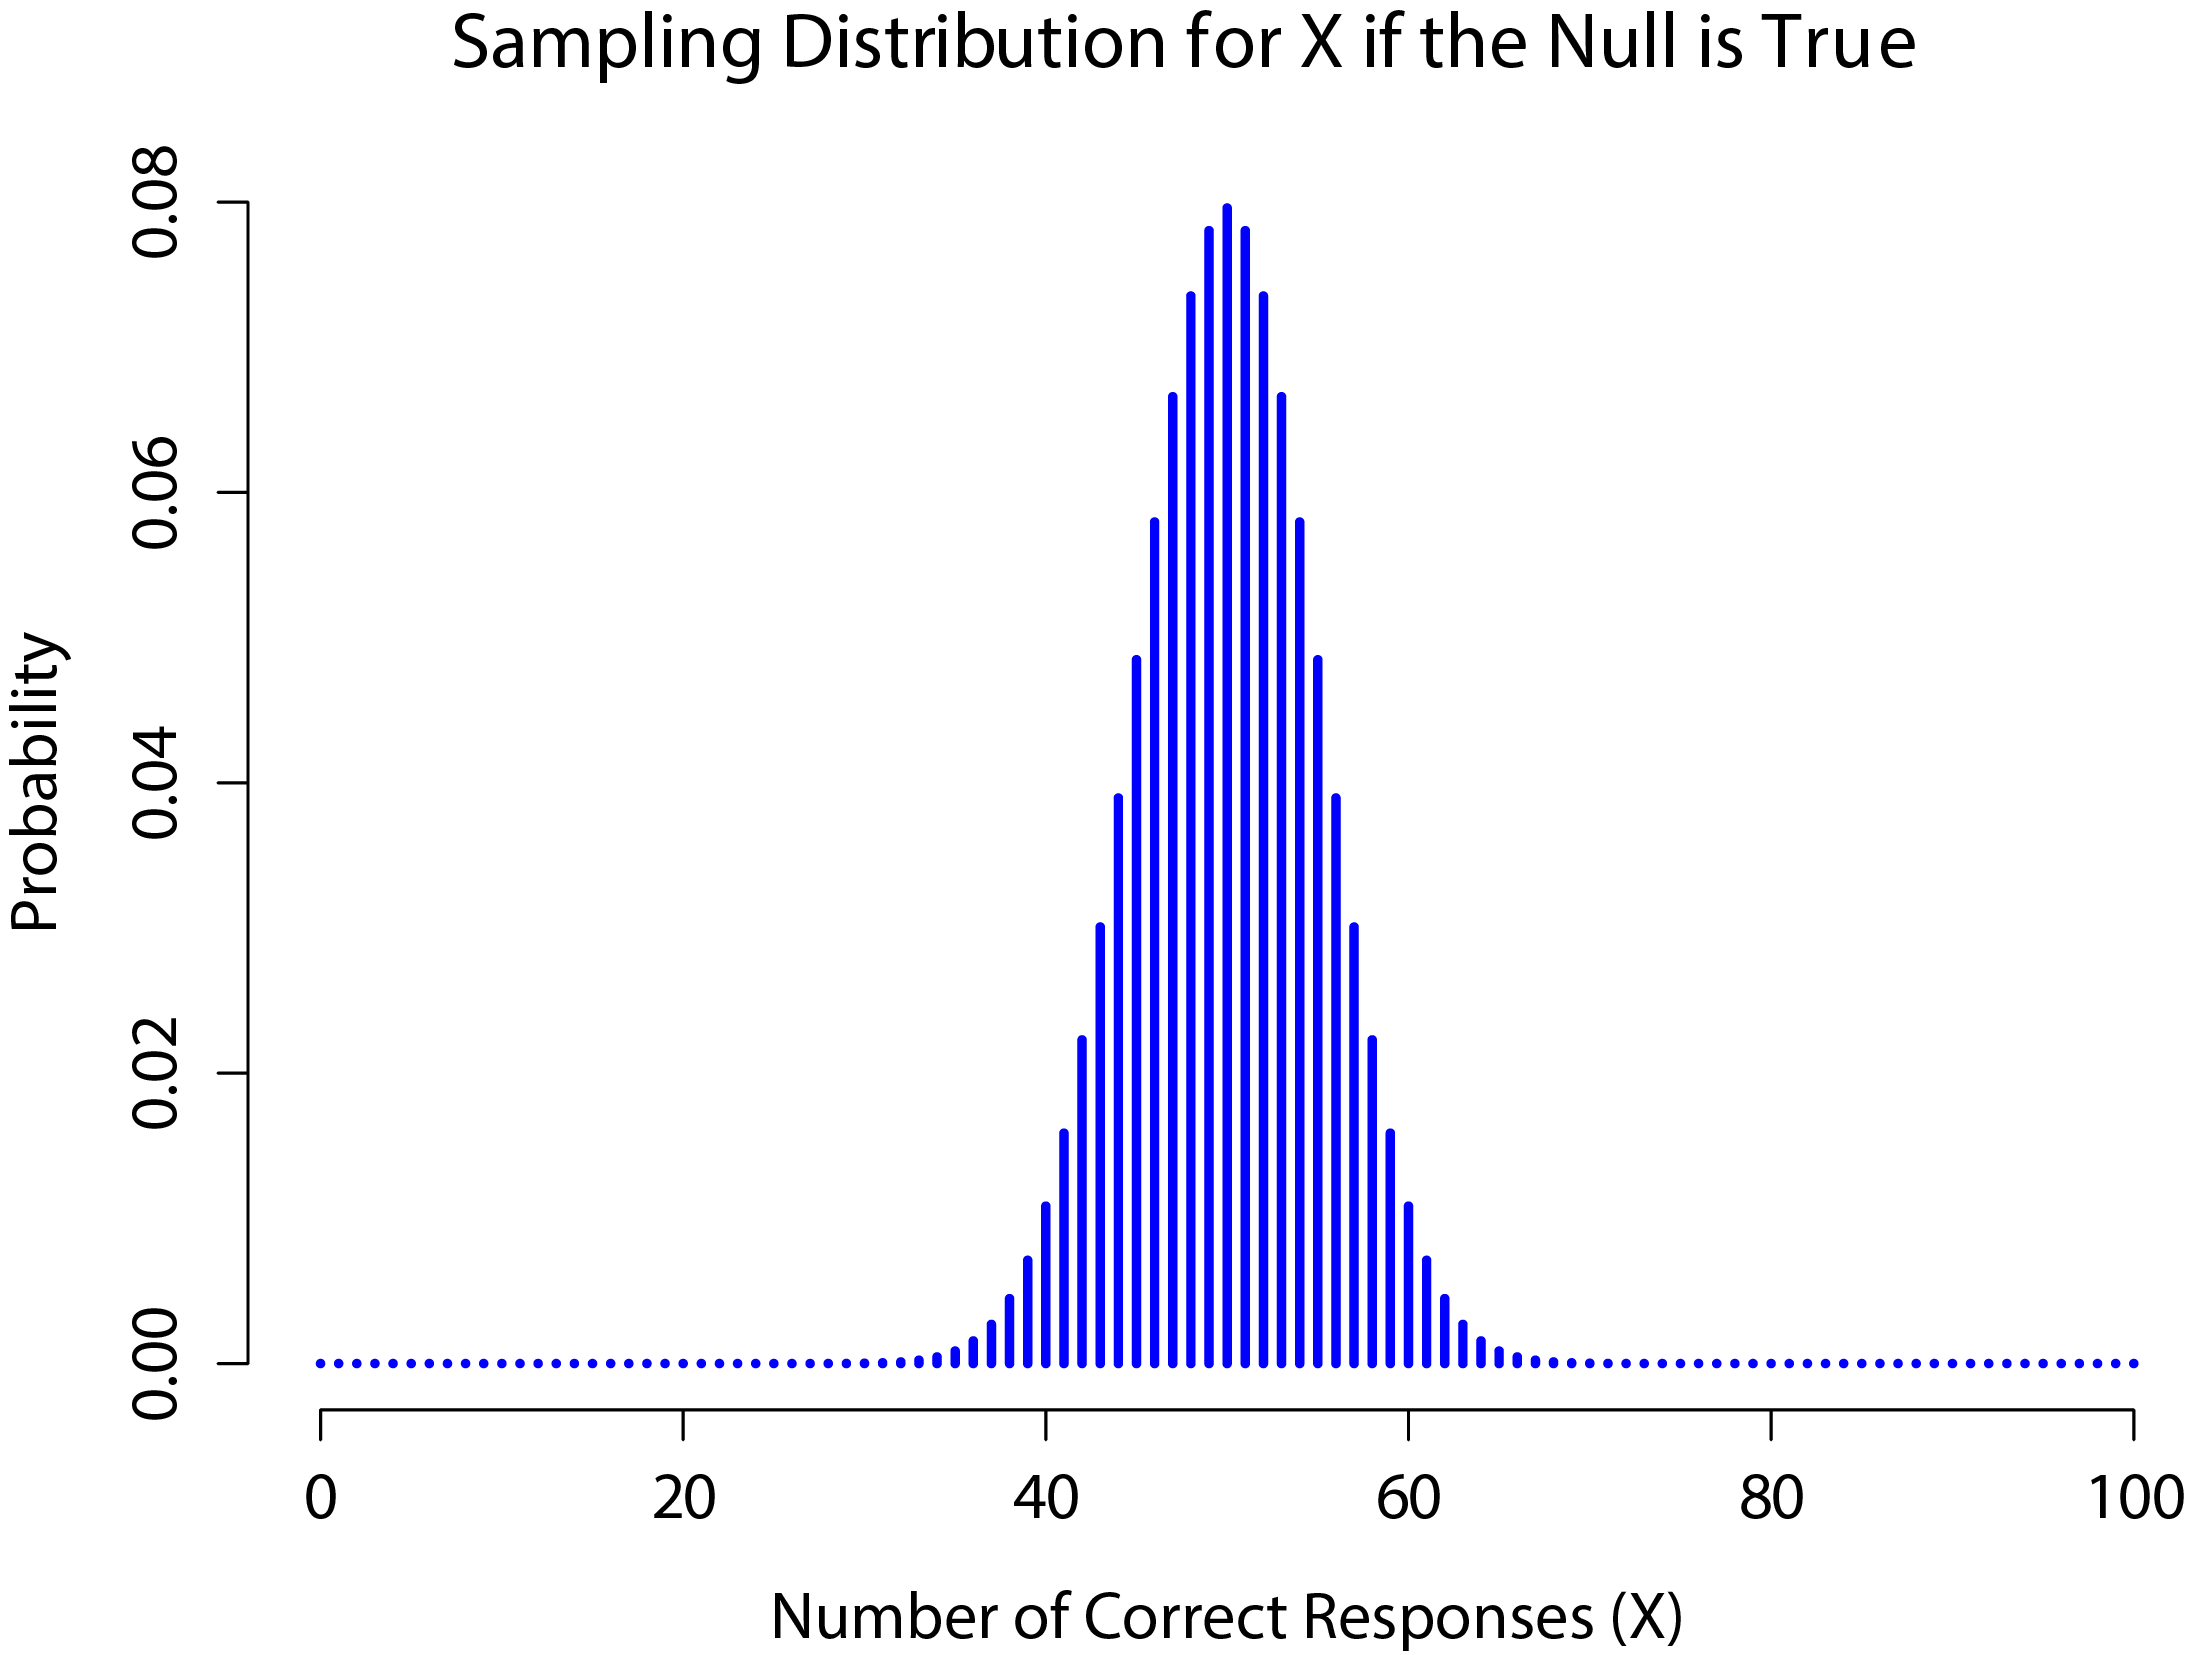
\includegraphics[width=1\linewidth]{img/nhst/samplingDist} 

}

\caption{The sampling distribution for our test statistic $X$ when the null hypothesis is true. For our ESP scenario this is a binomial distribution. Not surprisingly, since the null hypothesis says that the probability of a correct response is $  heta = .5$, the sampling distribution says that the most likely value is 50 (out of 100) correct responses. Most of the probability mass lies between 40 and 60.}\label{fig:samplingdist}
\end{figure}

\hypertarget{decisionmaking}{%
\section{Making decisions}\label{decisionmaking}}

Okay, we're very close to being finished. We've constructed a test statistic (\(X\)) and we chose this test statistic in such a way that we're pretty confident that if \(X\) is close to \(N/2\) then we should retain the null, and if not we should reject it. The question that remains is this. Exactly which values of the test statistic should we associate with the null hypothesis, and exactly which values go with the alternative hypothesis? In my ESP study, for example, I've observed a value of \(X=62\). What decision should I make? Should I choose to believe the null hypothesis or the alternative hypothesis?

\hypertarget{critical-regions-and-critical-values}{%
\subsection{Critical regions and critical values}\label{critical-regions-and-critical-values}}

To answer this question we need to introduce the concept of a {\textbf{critical region}} for the test statistic \(X\). The critical region of the test corresponds to those values of \(X\) that would lead us to reject null hypothesis (which is why the critical region is also sometimes called the rejection region). How do we find this critical region? Well, let's consider what we know:

\begin{itemize}
\tightlist
\item
  \(X\) should be very big or very small in order to reject the null hypothesis.
\item
  If the null hypothesis is true, the sampling distribution of \(X\) is Binomial\((0.5, N)\).
\item
  If \(\alpha =.05\), the critical region must cover 5\% of this sampling distribution.
\end{itemize}

It's important to make sure you understand this last point. The critical region corresponds to those values of \(X\) for which we would reject the null hypothesis, and the sampling distribution in question describes the probability that we would obtain a particular value of \(X\) if the null hypothesis were actually true. Now, let's suppose that we chose a critical region that covers 20\% of the sampling distribution, and suppose that the null hypothesis is actually true. What would be the probability of incorrectly rejecting the null? The answer is of course 20\%. And, therefore, we would have built a test that had an \(\alpha\) level of \(0.2\). If we want \(\alpha = .05\), the critical region is only \emph{allowed} to cover 5\% of the sampling distribution of our test statistic.

As it turns out those three things uniquely solve the problem. Our critical region consists of the most \emph{extreme values}, known as the {\textbf{tails}} of the distribution. This is illustrated in Figure \ref{fig:crit2}. If we want \(\alpha = .05\) then our critical regions correspond to \(X \leq 40\) and \(X \geq 60\).\footnote{Strictly speaking, the test I just constructed has \(\alpha = .057\), which is a bit too generous. However, if I'd chosen 39 and 61 to be the boundaries for the critical region then the critical region only covers 3.5\% of the distribution. I figured that it makes more sense to use 40 and 60 as my critical values, and be willing to tolerate a 5.7\% type I error rate, since that's as close as I can get to a value of \(\alpha = .05\).} That is, if the number of people saying ``true'' is between 41 and 59, then we should retain the null hypothesis. If the number is between 0 to 40, or between 60 to 100, then we should reject the null hypothesis. The numbers 40 and 60 are often referred to as the {\textbf{critical values}} since they define the edges of the critical region.

\textbackslash begin\{figure\}

\{\centering 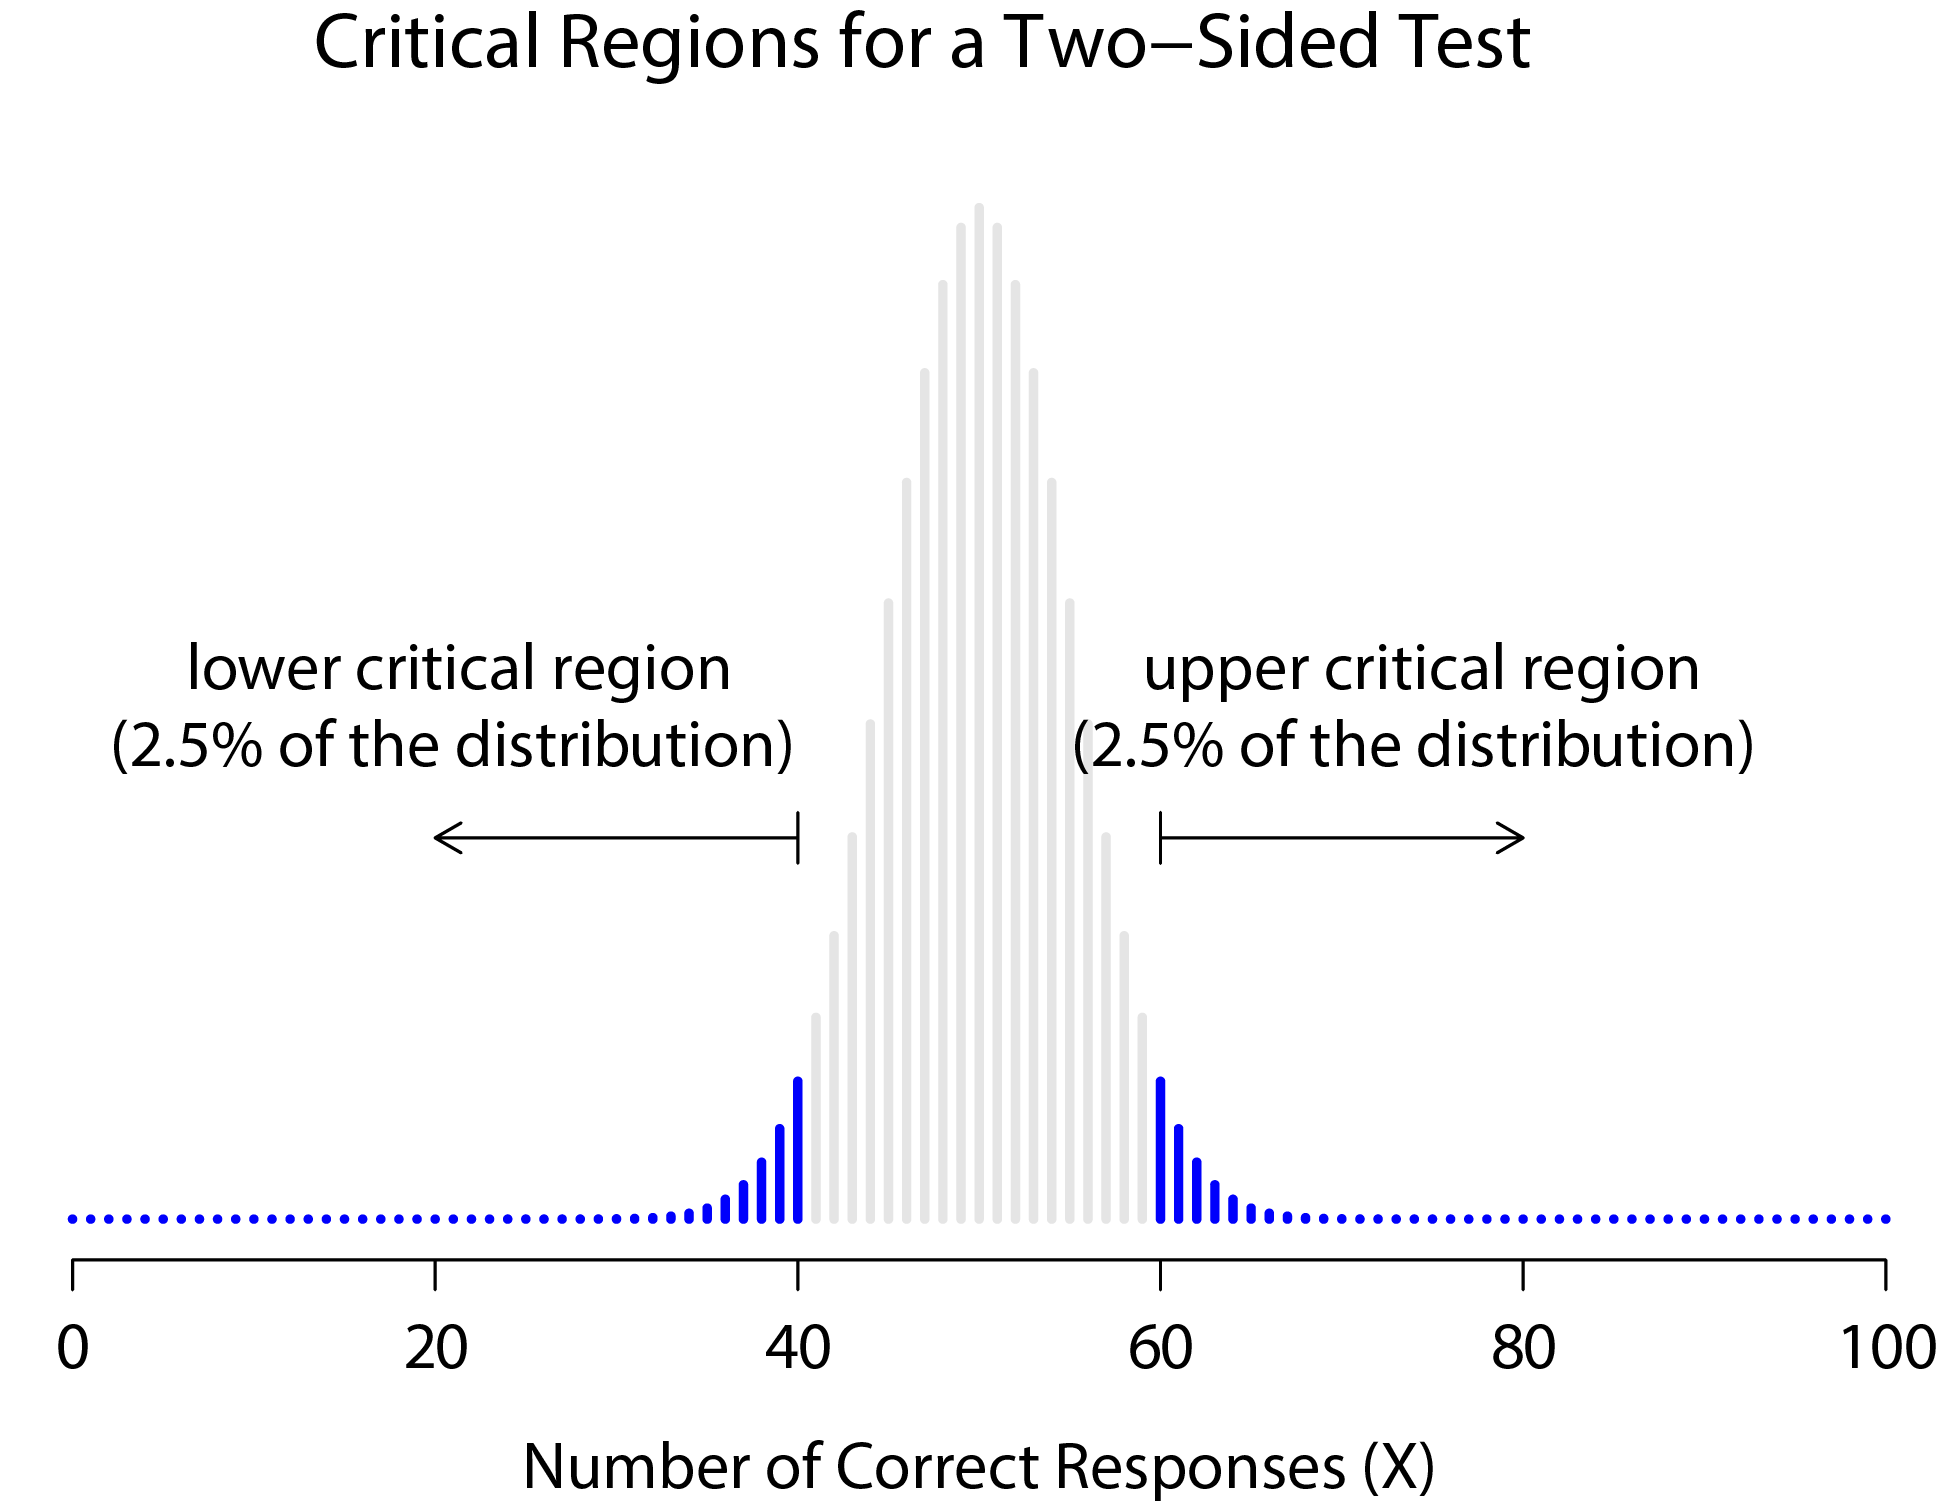
\includegraphics[width=1\linewidth]{img/nhst/rejectionRegion1}

\}

\textbackslash caption\{The critical region associated with the hypothesis test for the ESP study, for a hypothesis test with a significance level of \(\alpha = .05\). The plot shows the sampling distribution of \(X\) under the null hypothesis (i.e., same as Figure \ref{fig:samplingdist}). The grey bars correspond to those values of \(X\) for which we would retain the null hypothesis. The blue (darker shaded) bars show the critical region, those values of \(X\) for which we would reject the null. Because the alternative hypothesis is two sided (i.e., allows both \(\theta <.5\) and \(\theta >.5\)), the critical region covers both tails of the distribution. To ensure an \(\alpha\) level of \(.05\), we need to ensure that each of the two regions encompasses 2.5\% of the sampling distribution. \}\label{fig:crit2}
\textbackslash end\{figure\}

At this point, our hypothesis test is essentially complete:

\begin{enumerate}
\def\labelenumi{\arabic{enumi}.}
\tightlist
\item
  we choose an \(\alpha\) level (e.g., \(\alpha = .05\);
\item
  come up with some test statistic (e.g., \(X\)) that does a good job (in some meaningful sense) of comparing \(H_0\) to \(H_1\);
\item
  figure out the sampling distribution of the test statistic on the assumption that the null hypothesis is true (in this case, binomial); and then
\item
  calculate the critical region that produces an appropriate \(\alpha\) level (0-40 and 60-100).
\end{enumerate}

All that we have to do now is calculate the value of the test statistic for the real data (e.g., \(X = 62\)) and then compare it to the critical values to make our decision. Since 62 is greater than the critical value of 60 we would reject the null hypothesis. Or, to phrase it slightly differently, we say that the test has produced a statistically {\textbf{significant}} result.

\hypertarget{a-note-on-statistical-significance}{%
\subsection{A note on statistical ``significance''}\label{a-note-on-statistical-significance}}

~~~~~~\emph{Like other occult techniques of divination, the statistical method has a private jargon deliberately contrived to obscure its methods from non-practitioners.}\\
\hspace*{0.333em}\hspace*{0.333em}\hspace*{0.333em}\hspace*{0.333em}\hspace*{0.333em}\hspace*{0.333em}\hspace*{0.333em}\hspace*{0.333em}\hspace*{0.333em}\hspace*{0.333em}\hspace*{0.333em}\hspace*{0.333em}\hspace*{0.333em}\hspace*{0.333em}\hspace*{0.333em}\hspace*{0.333em}\hspace*{0.333em}\hspace*{0.333em}\hspace*{0.333em}\hspace*{0.333em}\hspace*{0.333em}\hspace*{0.333em}\hspace*{0.333em}\hspace*{0.333em}\hspace*{0.333em}\hspace*{0.333em}\hspace*{0.333em}\hspace*{0.333em}\hspace*{0.333em}\hspace*{0.333em}-- Attributed to G. O. Ashley\footnote{The internet seems fairly convinced that Ashley said this, though I can't for the life of me find anyone willing to give a source for the claim.}

A very brief digression is in order at this point, regarding the word ``significant.'' The concept of statistical significance is actually a very simple one, but has a very unfortunate name. If the data allow us to reject the null hypothesis, we say that ``the result is \emph{statistically significant},'' which is often shortened to ``the result is significant.'' This terminology is rather old and dates back to a time when ``significant'' just meant something like ``indicated,'' rather than its modern meaning which is much closer to ``important.'' As a result, a lot of modern readers get very confused when they start learning statistics because they think that a ``significant result'' must be an important one. It doesn't mean that at all. All that ``statistically significant'' means is that the data allowed us to reject a null hypothesis. Whether or not the result is actually important in the real world is a very different question, and depends on all sorts of other things.

\hypertarget{onesidedtests}{%
\subsection{The difference between one sided and two sided tests}\label{onesidedtests}}

There's one more thing I want to point out about the hypothesis test that I've just constructed. If we take a moment to think about the statistical hypotheses I've been using,
\[
\begin{array}{cc}
H_0 : & \theta = .5 \\
H_1 : & \theta \neq .5 
\end{array}
\]
we notice that the alternative hypothesis covers \emph{both} the possibility that \(\theta < .5\) and the possibility that \(\theta > .5\). This makes sense if I really think that ESP could produce either better-than-chance performance \emph{or} worse-than-chance performance (and there are some people who think that). In statistical language this is an example of a {\textbf{two-sided test}}. It's called this because the alternative hypothesis covers the area on both ``sides'' of the null hypothesis, and as a consequence the critical region of the test covers both tails of the sampling distribution (2.5\% on either side if \(\alpha =.05\)), as illustrated earlier in Figure \ref{fig:crit2}.

However, that's not the only possibility. I might only be willing to believe in ESP if it produces better than chance performance. If so, then my alternative hypothesis would only covers the possibility that \(\theta > .5\), and as a consequence the null hypothesis now becomes \(\theta \leq .5\)
\[
\begin{array}{cc}
H_0 : & \theta \leq .5 \\
H_1 : & \theta > .5 
\end{array}
\]
When this happens, we have what's called a {\textbf{one-sided test}} and the critical region only covers one tail of the sampling distribution. This is illustrated in Figure \ref{fig:crit1}.

\textbackslash begin\{figure\}

\{\centering 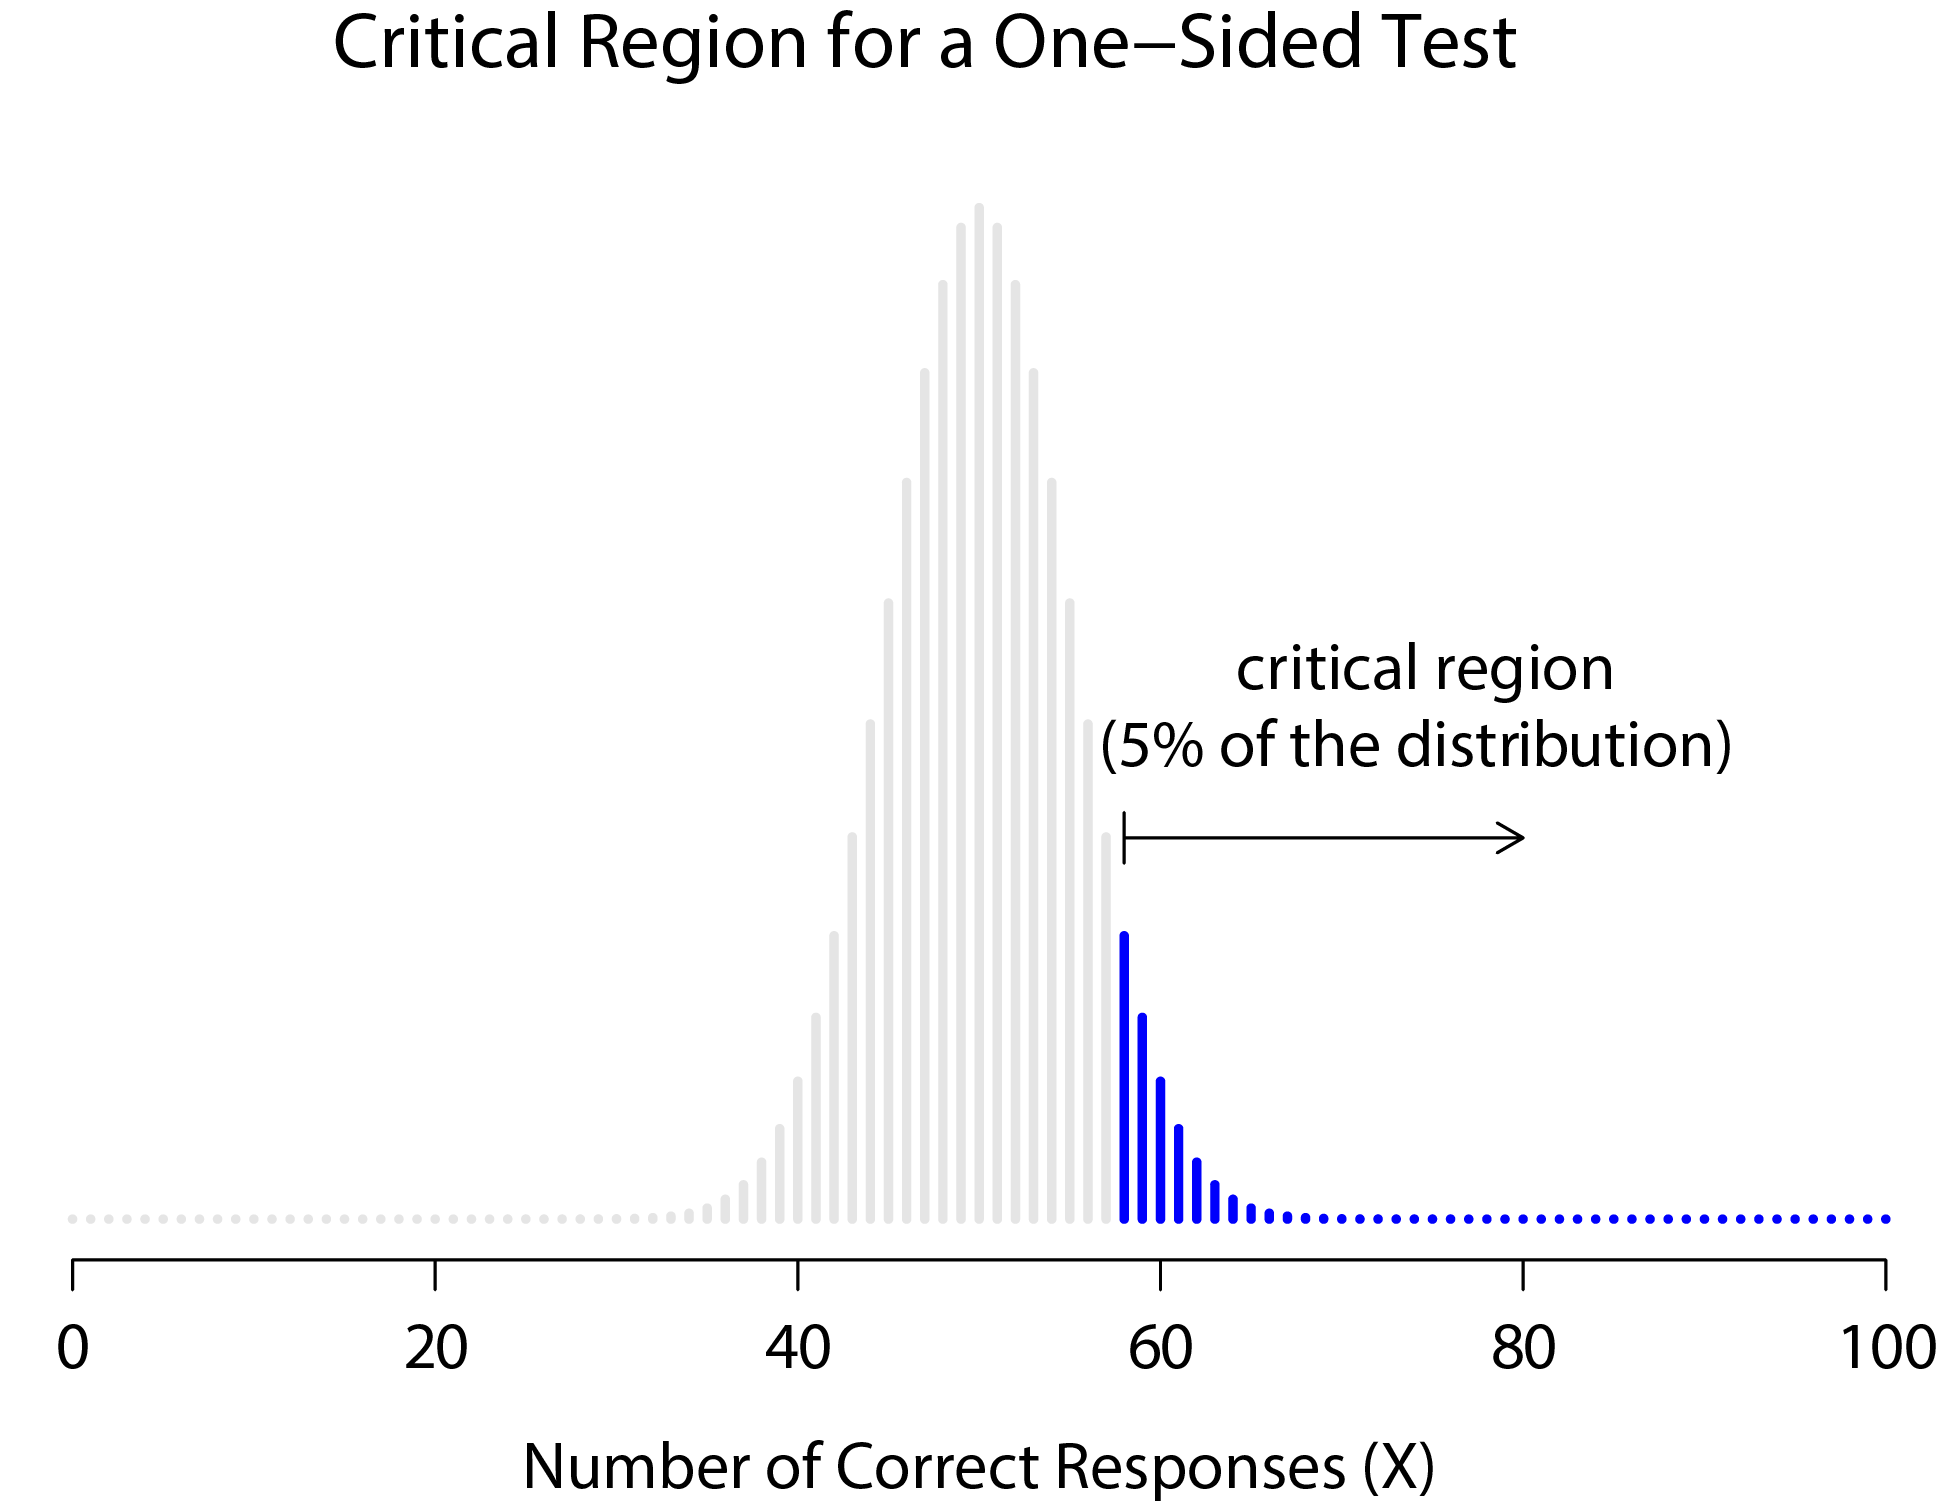
\includegraphics[width=1\linewidth]{img/nhst/rejectionRegion2}

\}

\textbackslash caption\{The critical region for a one sided test. In this case, the alternative hypothesis is that \(\theta > .5\) so we would only reject the null hypothesis for large values of \(X\). As a consequence, the critical region only covers the upper tail of the sampling distribution, specifically the upper 5\% of the distribution. Contrast this to the two-sided version in Figure \ref{fig:crit2}.\}\label{fig:crit1}
\textbackslash end\{figure\}

\hypertarget{pvalue}{%
\section{\texorpdfstring{The \(p\) value of a test}{The p value of a test}}\label{pvalue}}

In one sense, our hypothesis test is complete. We've constructed a test statistic, figured out its sampling distribution if the null hypothesis is true, and then constructed the critical region for the test. Nevertheless, I've actually omitted the most important number of all, {\textbf{the \(p\) value}}. It is to this topic that we now turn. There are two somewhat different ways of interpreting a \(p\) value, one proposed by Sir Ronald Fisher and the other by Jerzy Neyman. Both versions are legitimate, though they reflect very different ways of thinking about hypothesis tests. Most introductory textbooks tend to give Fisher's version only, but I think that's a bit of a shame. To my mind, Neyman's version is cleaner and actually better reflects the logic of the null hypothesis test. You might disagree though, so I've included both. I'll start with Neyman's version.

\hypertarget{a-softer-view-of-decision-making}{%
\subsection{A softer view of decision making}\label{a-softer-view-of-decision-making}}

One problem with the hypothesis testing procedure that I've described is that it makes no distinction at all between a result that is ``barely significant'' and those that are ``highly significant.'' For instance, in my ESP study the data I obtained only just fell inside the critical region, so I did get a significant effect but it was a pretty near thing. In contrast, suppose that I'd run a study in which \(X=97\) out of my \(N=100\) participants got the answer right. This would obviously be significant too but by a much larger margin, such that there's really no ambiguity about this at all. The procedure that I have already described makes no distinction between the two. If I adopt the standard convention of allowing \(\alpha = .05\) as my acceptable Type I error rate, then both of these are significant results.

This is where the \(p\) value comes in handy. To understand how it works, let's suppose that we ran lots of hypothesis tests on the same data set, but with a different value of \(\alpha\) in each case. When we do that for my original ESP data what we'd get is something like this

\begin{tabular}{c|c}
\hline
Value of \$\textbackslash{}alpha\$ & Reject the null?\\
\hline
0.05 & Yes\\
\hline
0.04 & Yes\\
\hline
0.03 & Yes\\
\hline
0.02 & No\\
\hline
0.01 & No\\
\hline
\end{tabular}

When we test the ESP data (\(X=62\) successes out of \(N=100\) observations), using \(\alpha\) levels of .03 and above, we'd always find ourselves rejecting the null hypothesis. For \(\alpha\) levels of .02 and below we always end up retaining the null hypothesis. Therefore, somewhere between .02 and .03 there must be a smallest value of \(\alpha\) that would allow us to reject the null hypothesis for this data. This is the \(p\) value. As it turns out the ESP data has \(p = .021\). In short,

\begin{quote}
\(p\) is defined to be the smallest Type I error rate (\(\alpha\)) that you have to be willing to tolerate if you want to reject the null hypothesis.
\end{quote}

If it turns out that \(p\) describes an error rate that you find intolerable, then you must retain the null. If you're comfortable with an error rate equal to \(p\), then it's okay to reject the null hypothesis in favour of your preferred alternative.

In effect, \(p\) is a summary of all the possible hypothesis tests that you could have run, taken across all possible \(\alpha\) values. And as a consequence it has the effect of ``softening'' our decision process. For those tests in which \(p \leq \alpha\) you would have rejected the null hypothesis, whereas for those tests in which \(p > \alpha\) you would have retained the null. In my ESP study I obtained \(X=62\) and as a consequence I've ended up with \(p = .021\). So the error rate I have to tolerate is 2.1\%. In contrast, suppose my experiment had yielded \(X=97\). What happens to my \(p\) value now? This time it's shrunk to \(p = 1.36 \times 10^{-25}\), which is a tiny, tiny\footnote{That's \(p = .000000000000000000000000136\) for folks that don't like scientific notation!} Type I error rate. For this second case I would be able to reject the null hypothesis with a lot more confidence, because I only have to be ``willing'' to tolerate a type I error rate of about 1 in 10 trillion trillion in order to justify my decision to reject.

\hypertarget{the-probability-of-extreme-data}{%
\subsection{The probability of extreme data}\label{the-probability-of-extreme-data}}

The second definition of the \(p\)-value comes from Sir Ronald Fisher, and it's actually this one that you tend to see in most introductory statistics textbooks. Notice how, when I constructed the critical region, it corresponded to the \emph{tails} (i.e., extreme values) of the sampling distribution? That's not a coincidence, almost all ``good'' tests have this characteristic (good in the sense of minimising our type II error rate, \(\beta\)). The reason for that is that a good critical region almost always corresponds to those values of the test statistic that are least likely to be observed if the null hypothesis is true. If this rule is true, then we can define the \(p\)-value as the probability that we would have observed a test statistic that is at least as extreme as the one we actually did get. In other words, if the data are extremely implausible according to the null hypothesis, then the null hypothesis is probably wrong.

\hypertarget{a-common-mistake}{%
\subsection{A common mistake}\label{a-common-mistake}}

Okay, so you can see that there are two rather different but legitimate ways to interpret the \(p\) value, one based on Neyman's approach to hypothesis testing and the other based on Fisher's. Unfortunately, there is a third explanation that people sometimes give, especially when they're first learning statistics, and it is \emph{absolutely and completely wrong}. This mistaken approach is to refer to the \(p\) value as ``the probability that the null hypothesis is true.'' It's an intuitively appealing way to think, but it's wrong in two key respects. First, null hypothesis testing is a frequentist tool and the frequentist approach to probability does \emph{not} allow you to assign probabilities to the null hypothesis. According to this view of probability, the null hypothesis is either true or it is not, it cannot have a ``5\% chance'' of being true. Second, even within the Bayesian approach, which does let you assign probabilities to hypotheses, the \(p\) value would not correspond to the probability that the null is true. This interpretation is entirely inconsistent with the mathematics of how the \(p\) value is calculated. Put bluntly, despite the intuitive appeal of thinking this way, there is \textbf{no} justification for interpreting a \(p\) value this way. Never do it.

\hypertarget{writeup}{%
\section{Reporting the results of a hypothesis test}\label{writeup}}

When writing up the results of a hypothesis test there's usually several pieces of information that you need to report, but it varies a fair bit from test to test. Throughout the rest of the book I'll spend a little time talking about how to report the results of different tests (see Section \ref{chisqreport} for a particularly detailed example), so that you can get a feel for how it's usually done. However, regardless of what test you're doing, the one thing that you always have to do is say something about the \(p\) value and whether or not the outcome was significant.

The fact that you have to do this is unsurprising, it's the whole point of doing the test. What might be surprising is the fact that there is some contention over exactly how you're supposed to do it. Leaving aside those people who completely disagree with the entire framework underpinning null hypothesis testing, there's a certain amount of tension that exists regarding whether or not to report the exact \(p\) value that you obtained, or if you should state only that \(p < \alpha\) for a significance level that you chose in advance (e.g., \(p<.05\)).

\hypertarget{the-issue}{%
\subsection{The issue}\label{the-issue}}

To see why this is an issue, the key thing to recognise is that \(p\) values are \emph{terribly} convenient. In practice, the fact that we can compute a \(p\) value means that we don't actually have to specify any \(\alpha\) level at all in order to run the test. Instead, what you can do is calculate your \(p\) value and interpret it directly. If you get \(p = .062\), then it means that you'd have to be willing to tolerate a Type I error rate of 6.2\% to justify rejecting the null. If you personally find 6.2\% intolerable then you retain the null. Therefore, the argument goes, why don't we just report the actual \(p\) value and let the reader make up their own minds about what an acceptable Type I error rate is? This approach has the big advantage of ``softening'' the decision making process. In fact, if you accept the Neyman definition of the \(p\) value, that's the whole point of the \(p\) value. We no longer have a fixed significance level of \(\alpha = .05\) as a bright line separating ``accept'' from ``reject'' decisions, and this removes the rather pathological problem of being forced to treat \(p = .051\) in a fundamentally different way to \(p = .049\).

This flexibility is both the advantage and the disadvantage to the \(p\) value. The reason why a lot of people don't like the idea of reporting an exact \(p\) value is that it gives the researcher a bit \emph{too much} freedom. In particular, it lets you change your mind about what error tolerance you're willing to put up with \emph{after} you look at the data. For instance, consider my ESP experiment. Suppose I ran my test and ended up with a \(p\) value of .09. Should I accept or reject? Now, to be honest, I haven't yet bothered to think about what level of Type I error I'm ``really'' willing to accept. I don't have an opinion on that topic. But I \emph{do} have an opinion about whether or not ESP exists, and I \emph{definitely} have an opinion about whether my research should be published in a reputable scientific journal. And amazingly, now that I've looked at the data I'm starting to think that a 9\% error rate isn't so bad, especially when compared to how annoying it would be to have to admit to the world that my experiment has failed. So, to avoid looking like I just made it up after the fact, I now say that my \(\alpha\) is .1, with the argument that a 10\% type I error rate isn't too bad and at that level my test is significant! I win.

In other words, the worry here is that I might have the best of intentions, and be the most honest of people, but the temptation to just ``shade'' things a little bit here and there is really, really strong. As anyone who has ever run an experiment can attest, it's a long and difficult process and you often get \emph{very} attached to your hypotheses. It's hard to let go and admit the experiment didn't find what you wanted it to find. And that's the danger here. If we use the ``raw'' \(p\)-value, people will start interpreting the data in terms of what they \emph{want} to believe, not what the data are actually saying and, if we allow that, why are we even bothering to do science at all? Why not let everyone believe whatever they like about anything, regardless of what the facts are? Okay, that's a bit extreme, but that's where the worry comes from. According to this view, you really \emph{must} specify your \(\alpha\) value in advance and then only report whether the test was significant or not. It's the only way to keep ourselves honest.

\hypertarget{two-proposed-solutions}{%
\subsection{Two proposed solutions}\label{two-proposed-solutions}}

In practice, it's pretty rare for a researcher to specify a single \(\alpha\) level ahead of time. Instead, the convention is that scientists rely on three standard significance levels: .05, .01 and .001. When reporting your results, you indicate which (if any) of these significance levels allow you to reject the null hypothesis. This is summarised in Table \ref{tab:pvaltable}. This allows us to soften the decision rule a little bit, since \(p<.01\) implies that the data meet a stronger evidential standard than \(p<.05\) would. Nevertheless, since these levels are fixed in advance by convention, it does prevent people choosing their \(\alpha\) level after looking at the data.

\begin{table}

\caption{\label{tab:pvaltable}A commonly adopted convention for reporting $p$ values: in many places it is conventional to report one of four different things (e.g., $p<.05$) as shown below. I've included the "significance stars" notation (i.e., a * indicates $p<.05$) because you sometimes see this notation produced by statistical software. It's also worth noting that some people will write *n.s.* (not significant) rather than $p>.05$.}
\centering
\begin{tabular}[t]{l|l|l|l}
\hline
Usual notation & Signif stars & English Translation & The null is...\\
\hline
\$p>.05\$ &  & The test wasn't significant & Retained\\
\hline
\$p<.05\$ & * & The test was significant at \$\textbackslash{}alpha\$ = .05 but not at  \$\textbackslash{}alpha =.01\$ or \$\textbackslash{}alpha = .001\$ & Rejected\\
\hline
\$p<.01\$ & ** & The test was significant at \$\textbackslash{}alpha\$ = .05  and \$\textbackslash{}alpha = .01\$ but not at  \$\textbackslash{}alpha = .001\$ & Rejected\\
\hline
\$p<.001\$ & *** & The test was significant at all levels & Rejected\\
\hline
\end{tabular}
\end{table}

Nevertheless, quite a lot of people still prefer to report exact \(p\) values. To many people, the advantage of allowing the reader to make up their own mind about how to interpret \(p = .06\) outweighs any disadvantages. In practice, however, even among those researchers who prefer exact \(p\) values it is quite common to just write \(p<.001\) instead of reporting an exact value for small \(p\). This is in part because a lot of software doesn't actually print out the \(p\) value when it's that small (e.g., SPSS just writes \(p = .000\) whenever \(p<.001\)), and in part because a very small \(p\) value can be kind of misleading. The human mind sees a number like .0000000001 and it's hard to suppress the gut feeling that the evidence in favour of the alternative hypothesis is a near certainty. In practice however, this is usually wrong. Life is a big, messy, complicated thing, and every statistical test ever invented relies on simplifications, approximations and assumptions. As a consequence, it's probably not reasonable to walk away from \emph{any} statistical analysis with a feeling of confidence stronger than \(p<.001\) implies. In other words, \(p<.001\) is really code for ``as far as \emph{this test} is concerned, the evidence is overwhelming.''

In light of all this, you might be wondering exactly what you should do. There's a fair bit of contradictory advice on the topic, with some people arguing that you should report the exact \(p\) value, and other people arguing that you should use the tiered approach illustrated in Table \ref{tab:pvaltable}. As a result, the best advice I can give is to suggest that you look at papers/reports written in your field and see what the convention seems to be. If there doesn't seem to be any consistent pattern, then use whichever method you prefer.

\hypertarget{runhyp}{%
\section{Running the hypothesis test in practice}\label{runhyp}}

At this point some of you might be wondering if this is a ``real'' hypothesis test, or just a toy example that I made up. It's real. In the previous discussion I built the test from first principles, thinking that it was the simplest possible problem that you might ever encounter in real life. However, this test already exists. It's called the \emph{binomial test}, and it's implemented by jamovi as one of the statistical analyses available when you hit the `Frequencies' button. To test the null hypothesis that the response probability is one-half \texttt{p\ =\ .5},\footnote{Note that the \texttt{p} here has nothing to do with a \(p\) value. The \texttt{p} argument in the jamovi binomial test corresponds to the probability of making a correct response, according to the null hypothesis. In other words, it's the \(\theta\) value.} and using data in which \texttt{x\ =\ 62} of \texttt{n\ =\ 100} people made the correct response, available in the \textbf{\texttt{binomialtest.omv}} data file, we get the results shown in Figure \ref{fig:binomialtest}.

\begin{figure}

{\centering 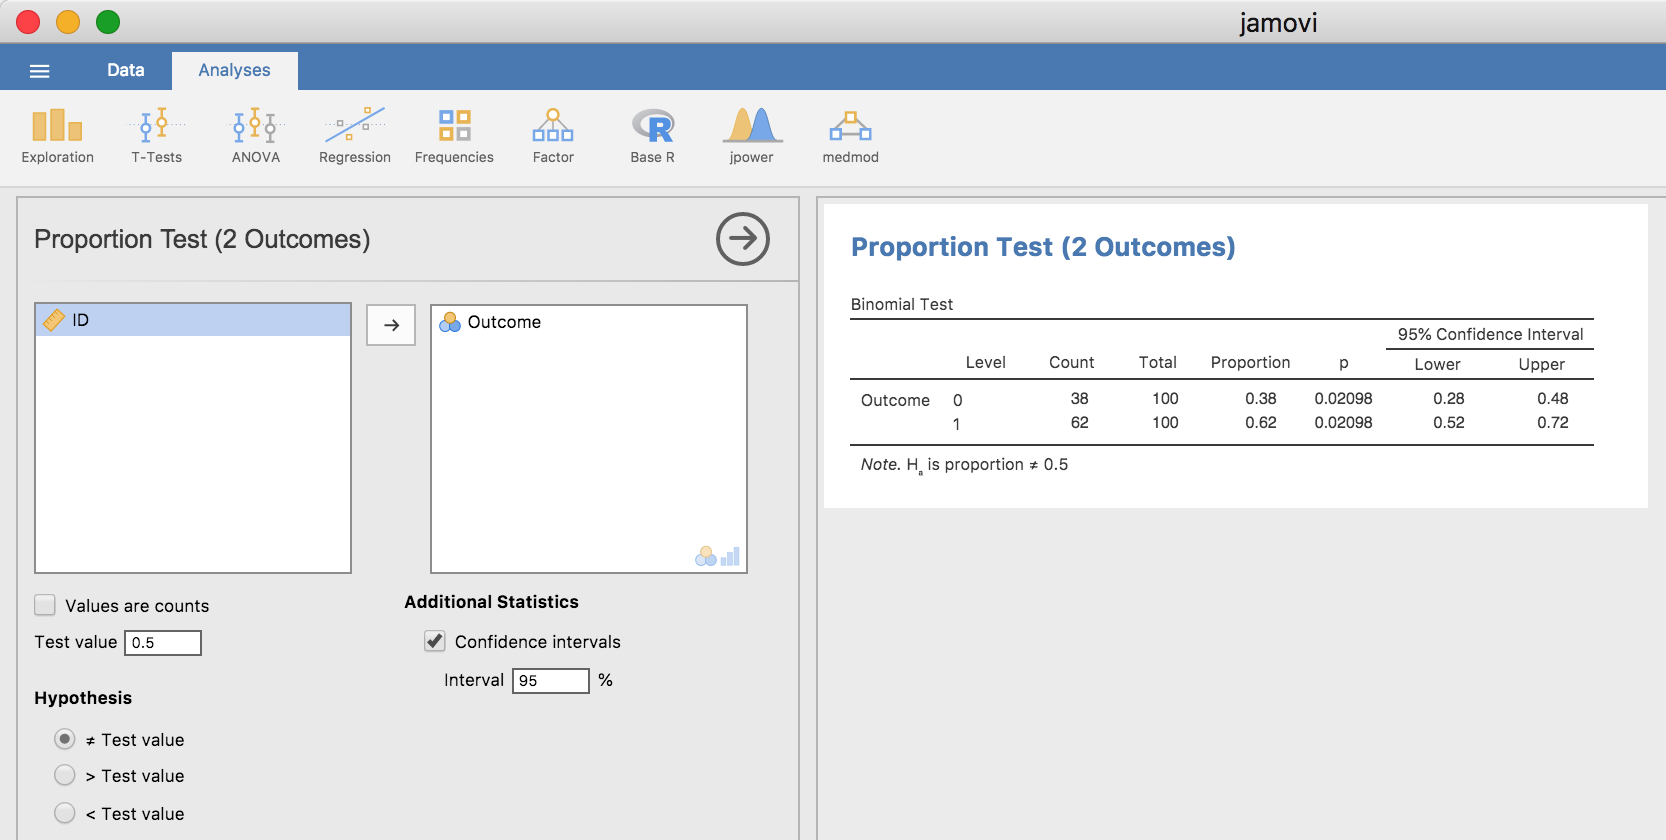
\includegraphics[width=1\linewidth]{img/nhst/binomialtest} 

}

\caption{Binomial test analysis and results in jamovi}\label{fig:binomialtest}
\end{figure}

Right now, this output looks pretty unfamiliar to you, but you can see that it's telling you more or less the right things. Specifically, the \(p\)-value of 0.02 is less than the usual choice of \(\alpha = .05\), so you can reject the null. We'll talk a lot more about how to read this sort of output as we go along, and after a while you'll hopefully find it quite easy to read and understand.

\hypertarget{effectsize}{%
\section{Effect size, sample size and power}\label{effectsize}}

In previous sections I've emphasised the fact that the major design principle behind statistical hypothesis testing is that we try to control our Type I error rate. When we fix \(\alpha = .05\) we are attempting to ensure that only 5\% of true null hypotheses are incorrectly rejected. However, this doesn't mean that we don't care about Type II errors. In fact, from the researcher's perspective, the error of failing to reject the null when it is actually false is an extremely annoying one. With that in mind, a secondary goal of hypothesis testing is to try to minimise \(\beta\), the Type II error rate, although we don't usually \emph{talk} in terms of minimising Type II errors. Instead, we talk about maximising the \emph{power} of the test. Since power is defined as \(1-\beta\), this is the same thing.

\hypertarget{the-power-function}{%
\subsection{The power function}\label{the-power-function}}

Let's take a moment to think about what a Type II error actually is. A Type II error occurs when the alternative hypothesis is true, but we are nevertheless unable to reject the null hypothesis. Ideally, we'd be able to calculate a single number \(\beta\) that tells us the Type II error rate, in the same way that we can set \(\alpha = .05\) for the Type I error rate. Unfortunately, this is a lot trickier to do. To see this, notice that in my ESP study the alternative hypothesis actually corresponds to lots of possible values of \(\theta\). In fact, the alternative hypothesis corresponds to every value of \(\theta\) \emph{except} 0.5. Let's suppose that the true probability of someone choosing the correct response is 55\% (i.e., \(\theta = .55\)). If so, then the \emph{true} sampling distribution for \(X\) is not the same one that the null hypothesis predicts, as the most likely value for \(X\) is now 55 out of 100. Not only that, the whole sampling distribution has now shifted, as shown in Figure \ref{fig:crit3}.

\begin{figure}

{\centering 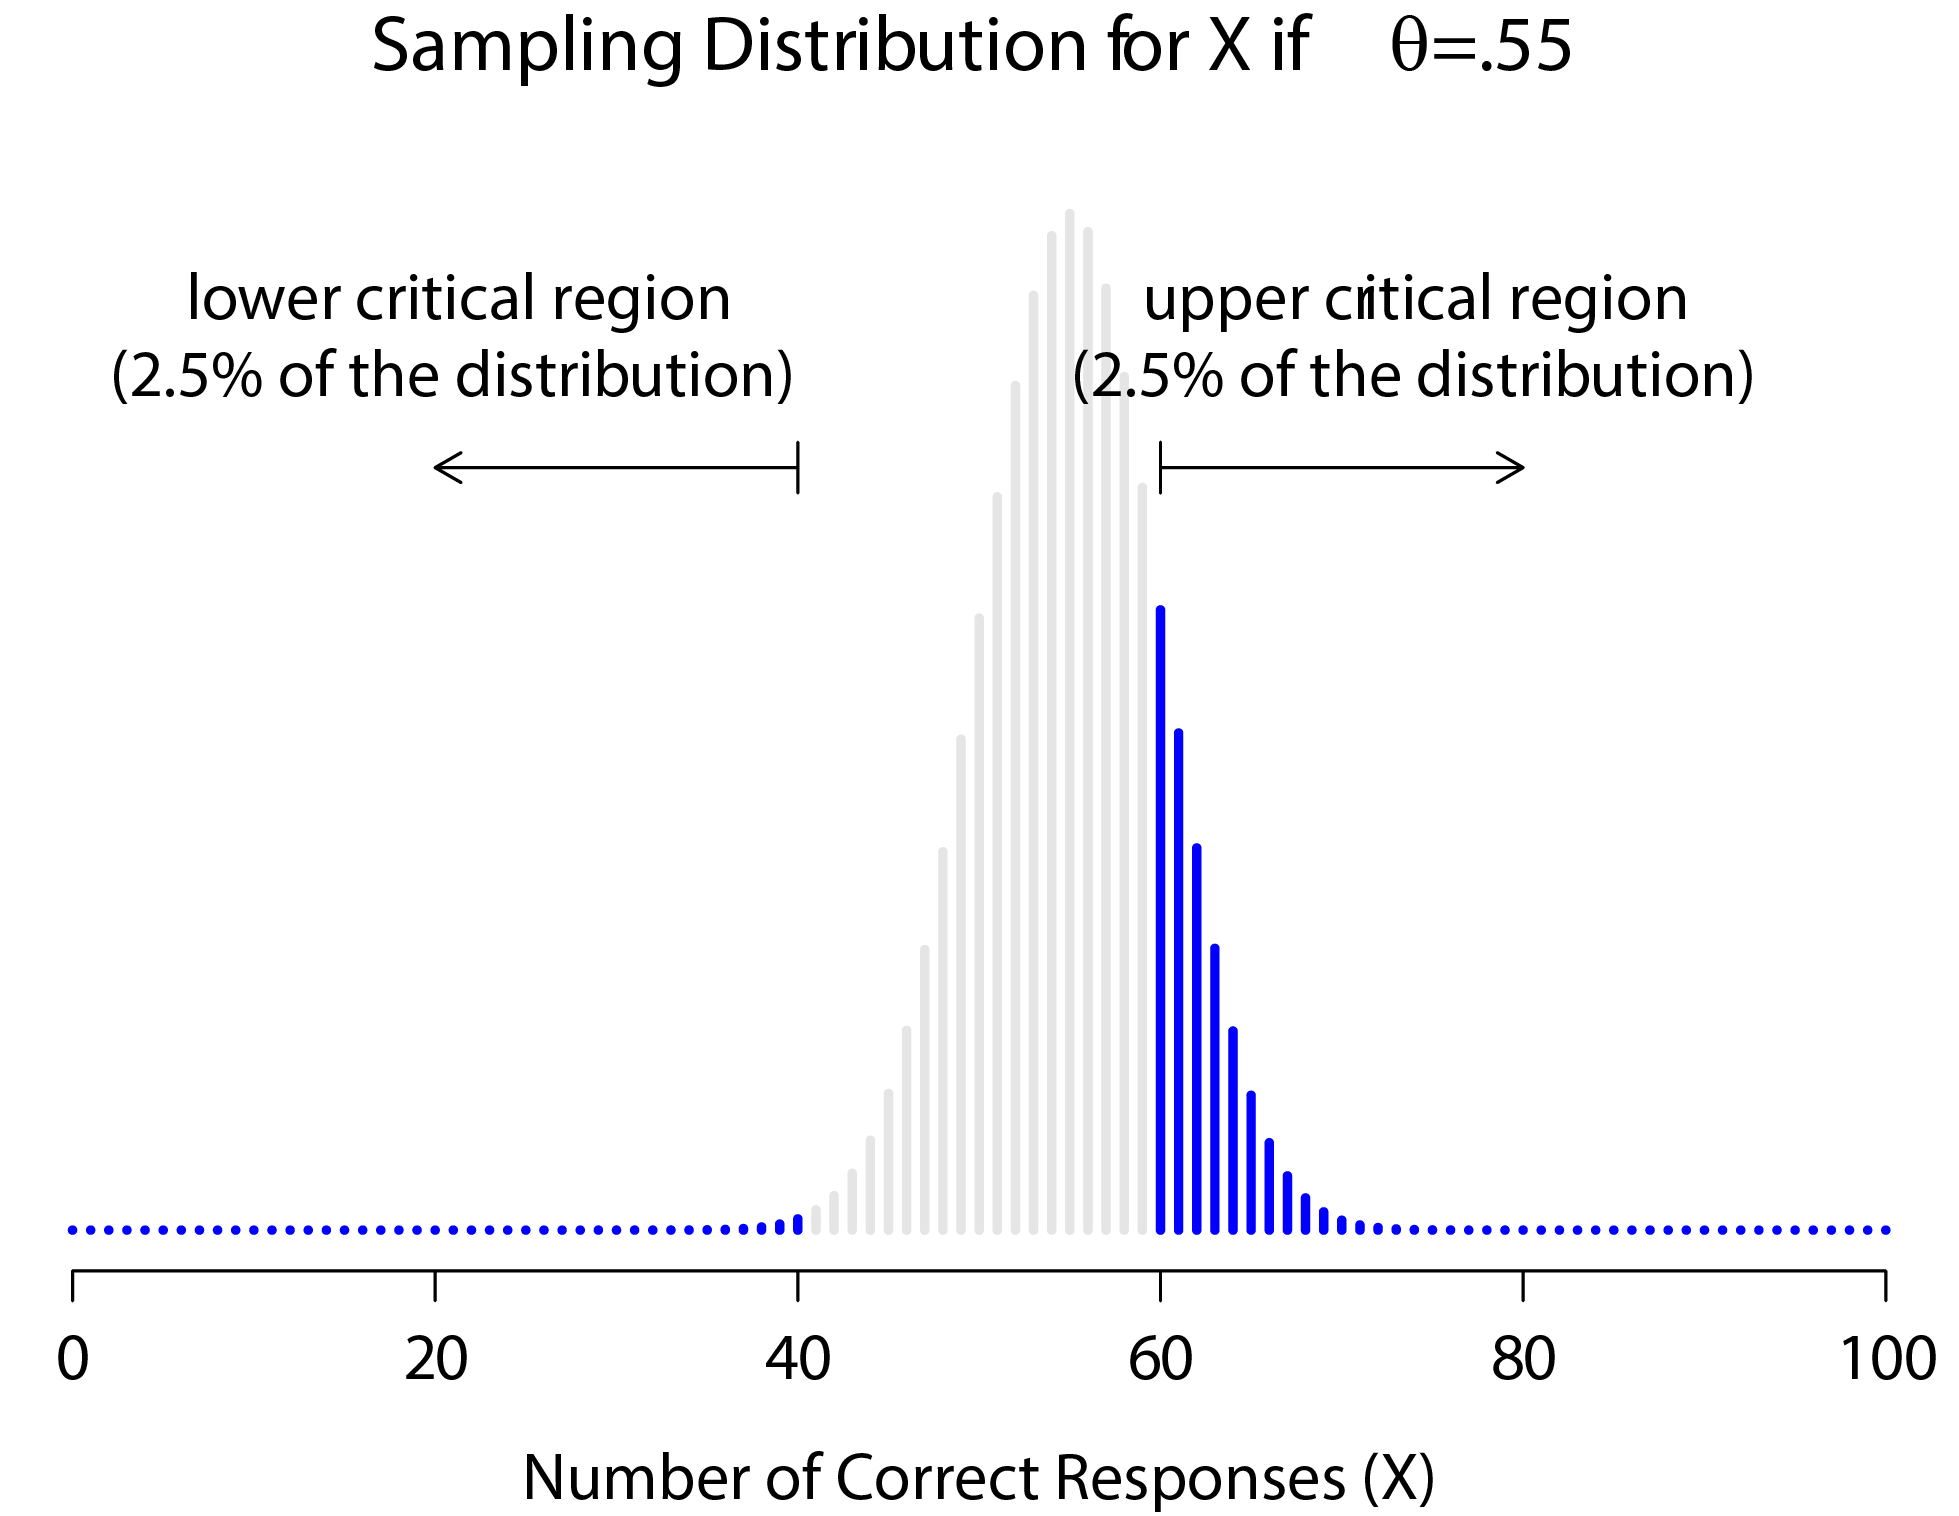
\includegraphics[width=1\linewidth]{img/nhst/rejectionRegion3} 

}

\caption{Sampling distribution under the *alternative* hypothesis for a population parameter value of $\theta = 0.55$. A reasonable proportion of the distribution lies in the rejection region.}\label{fig:crit3}
\end{figure}

The critical regions, of course, do not change. By definition the critical regions are based on what the null hypothesis predicts. What we're seeing in this figure is the fact that when the null hypothesis is wrong, a much larger proportion of the sampling distribution distribution falls in the critical region. And of course that's what should happen. The probability of rejecting the null hypothesis is larger when the null hypothesis is actually false! However \(\theta = .55\) is not the only possibility consistent with the alternative hypothesis. Let's instead suppose that the true value of \(\theta\) is actually 0.7. What happens to the sampling distribution when this occurs? The answer, shown in Figure \ref{fig:crit4}, is that almost the entirety of the sampling distribution has now moved into the critical region. Therefore, if \(\theta = 0.7\), the probability of us correctly rejecting the null hypothesis (i.e., the power of the test) is much larger than if \(\theta = 0.55\). In short, while \(\theta = .55\) and \(\theta = .70\) are both part of the alternative hypothesis, the Type II error rate is different.

\begin{figure}

{\centering 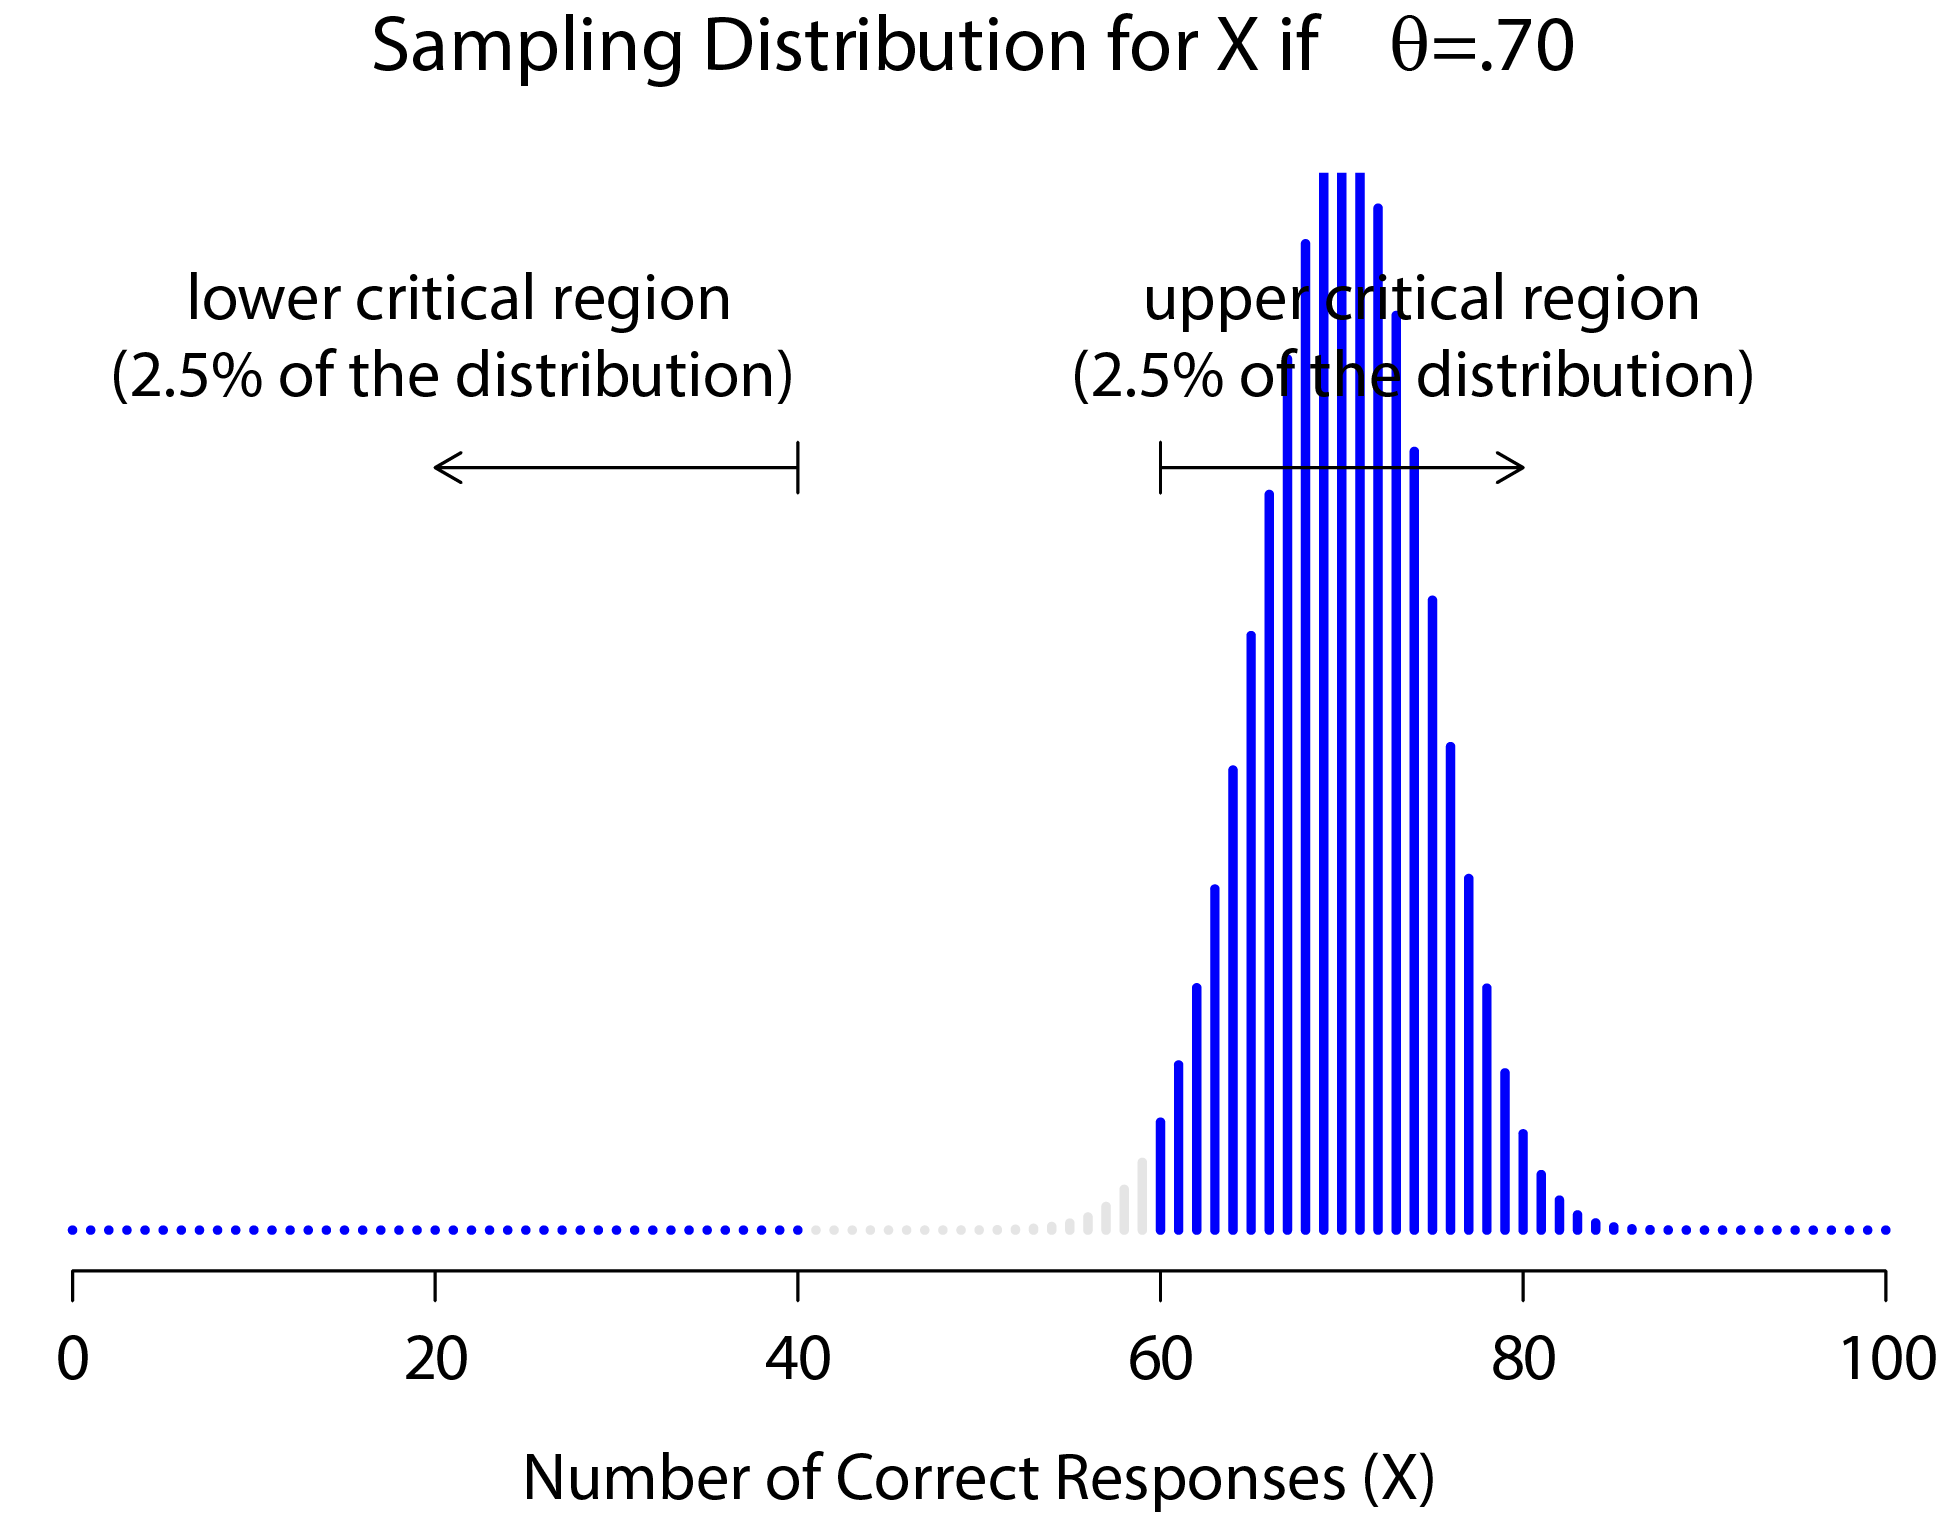
\includegraphics[width=1\linewidth]{img/nhst/rejectionRegion4} 

}

\caption{Sampling distribution under the *alternative* hypothesis for a population parameter value of $\theta = 0.70$. Almost all of the distribution lies in the rejection region.}\label{fig:crit4}
\end{figure}

What all this means is that the power of a test (i.e., \(1-\beta\)) depends on the true value of \(\theta\). To illustrate this, I've calculated the expected probability of rejecting the null hypothesis for all values of \(\theta\), and plotted it in Figure \ref{fig:powerfunction}. This plot describes what is usually called the {\textbf{power function}} of the test. It's a nice summary of how good the test is, because it actually tells you the power (\(1-\beta\)) for all possible values of \(\theta\). As you can see, when the true value of \(\theta\) is very close to 0.5, the power of the test drops very sharply, but when it is further away, the power is large.

\begin{figure}

{\centering 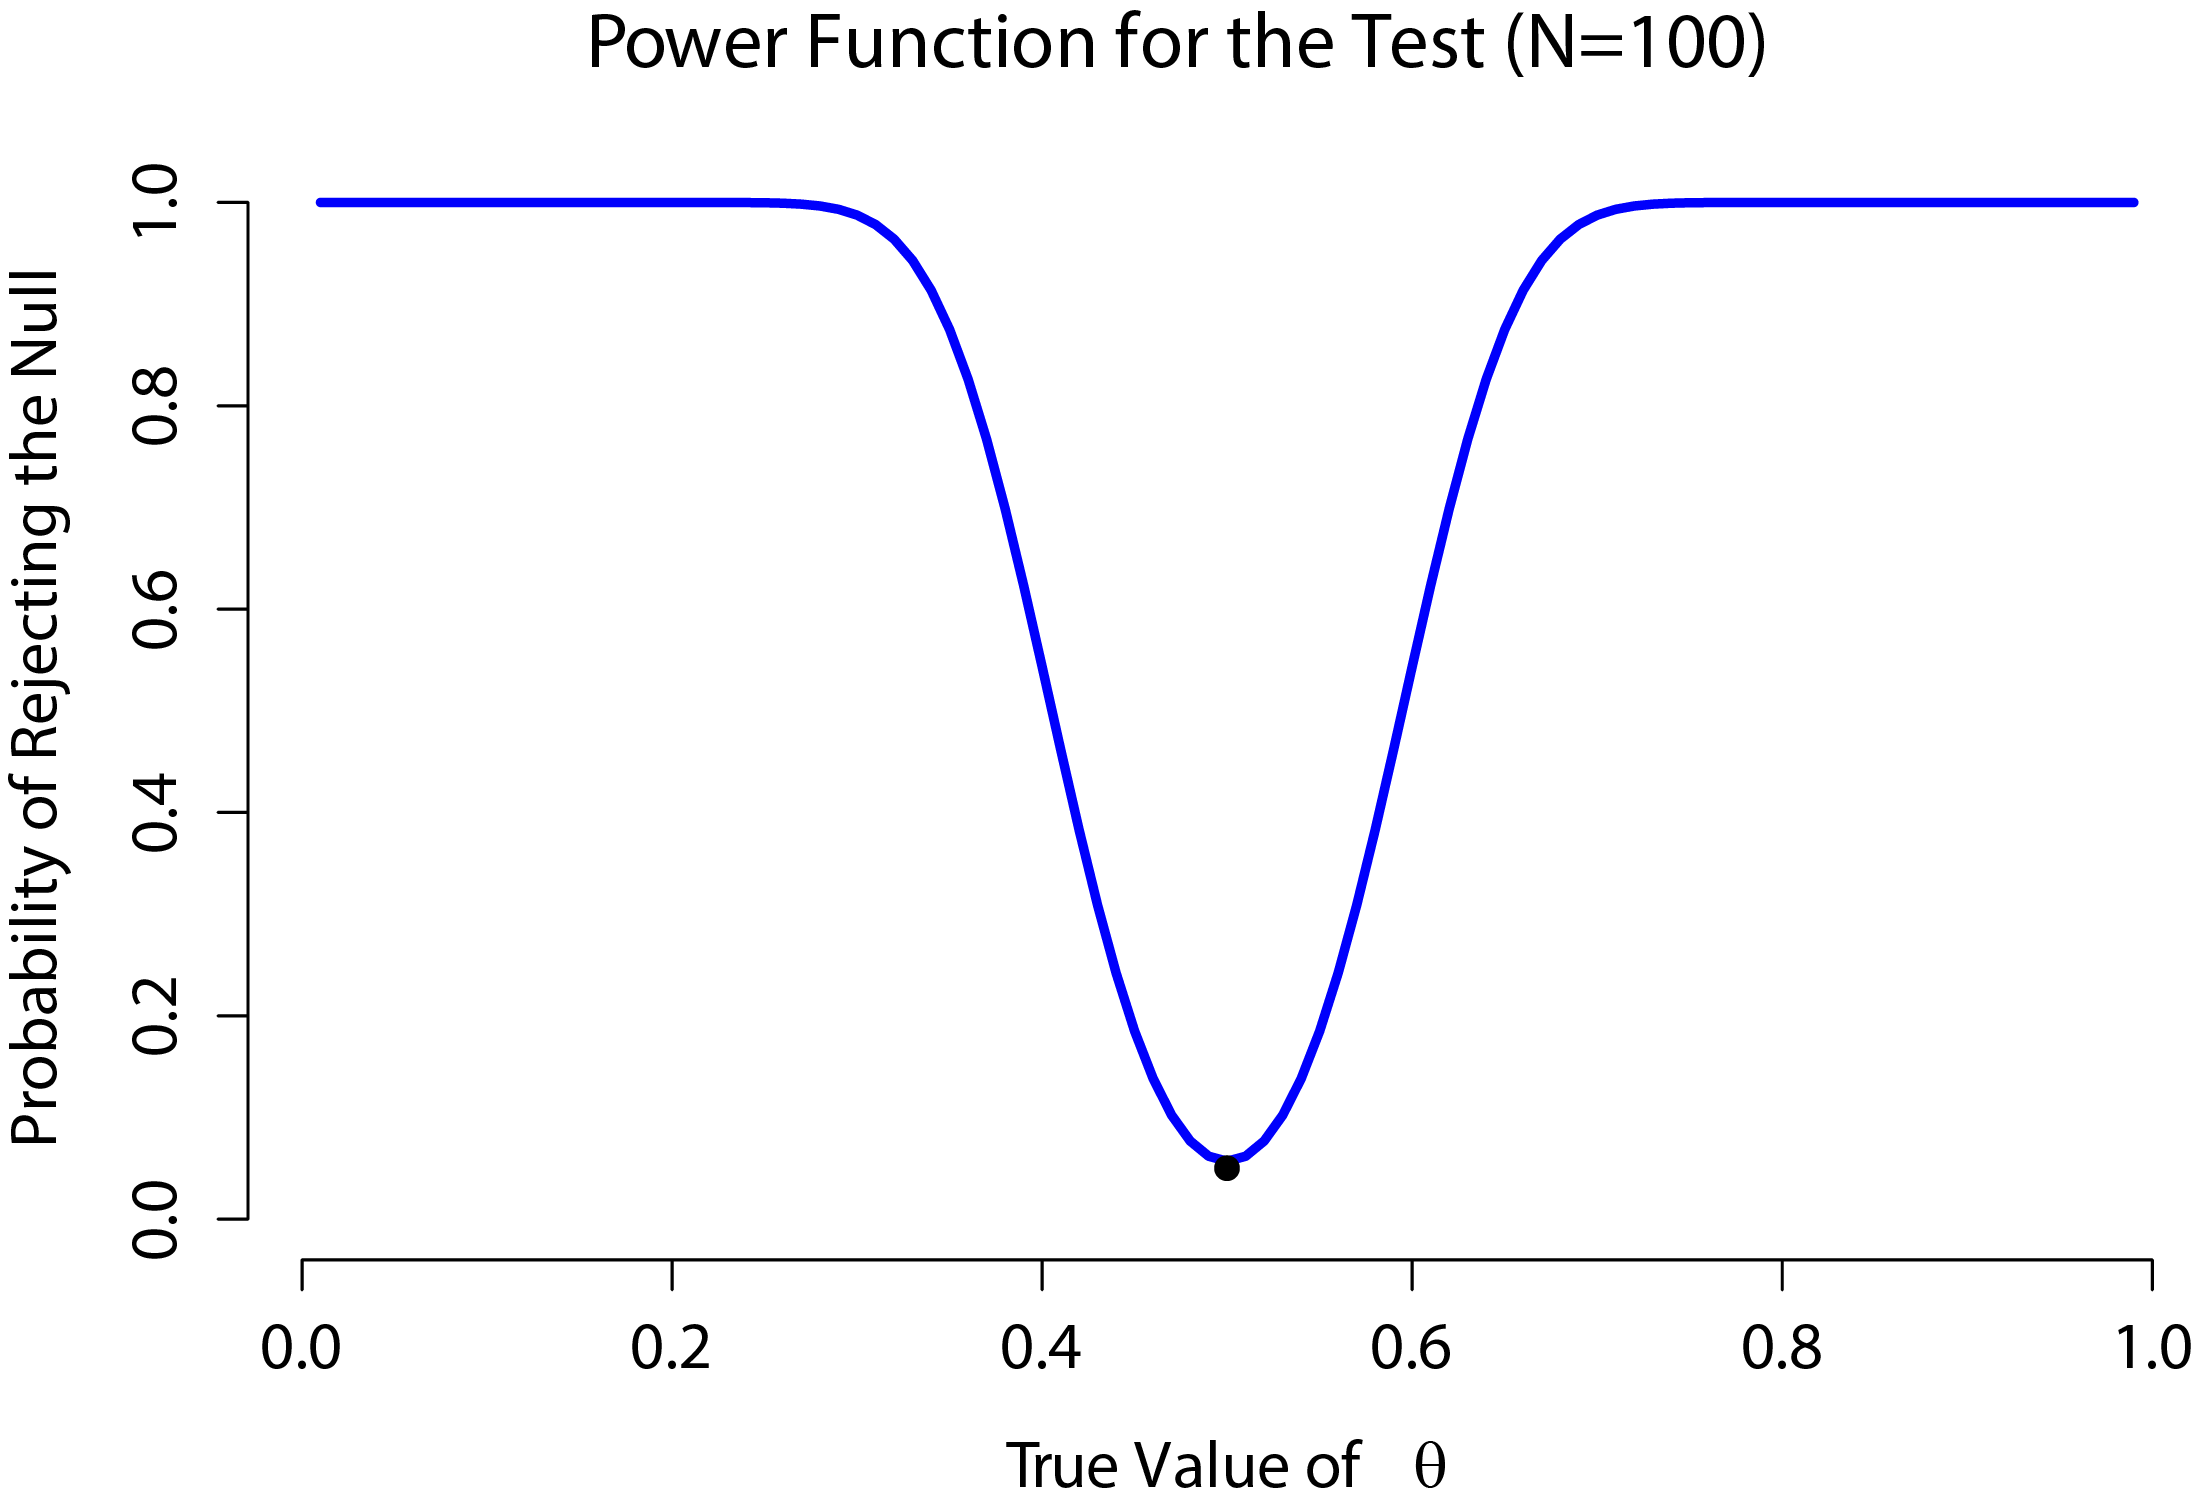
\includegraphics[width=1\linewidth]{img/nhst/powerTheta} 

}

\caption{The probability that we will reject the null hypothesis, plotted as a function of the true value of $\theta$. Obviously, the test is more powerful (greater chance of correct rejection) if the true value of $\theta$ is very different from the value that the null hypothesis specifies (i.e., $\theta=.5$). Notice that when $\theta$ actually is equal to .5 (plotted as a black dot), the null hypothesis is in fact true and rejecting the null hypothesis in this instance would be a Type I error.}\label{fig:powerfunction}
\end{figure}

\hypertarget{effect-size}{%
\subsection{Effect size}\label{effect-size}}

~~~~~~\emph{Since all models are wrong the scientist must be alert to what is importantly wrong. It is inappropriate to be concerned with mice when there are tigers abroad}\\
\hspace*{0.333em}\hspace*{0.333em}\hspace*{0.333em}\hspace*{0.333em}\hspace*{0.333em}\hspace*{0.333em}\hspace*{0.333em}\hspace*{0.333em}\hspace*{0.333em}\hspace*{0.333em}\hspace*{0.333em}\hspace*{0.333em}\hspace*{0.333em}\hspace*{0.333em}\hspace*{0.333em}\hspace*{0.333em}\hspace*{0.333em}\hspace*{0.333em}\hspace*{0.333em}\hspace*{0.333em}\hspace*{0.333em}\hspace*{0.333em}\hspace*{0.333em}\hspace*{0.333em}\hspace*{0.333em}\hspace*{0.333em}\hspace*{0.333em}\hspace*{0.333em}\hspace*{0.333em}\hspace*{0.333em}-- George Box (\protect\hyperlink{ref-Box1976}{Box, 1976}, p 792)

The plot shown in Figure \ref{fig:powerfunction} captures a fairly basic point about hypothesis testing. If the true state of the world is very different from what the null hypothesis predicts then your power will be very high, but if the true state of the world is similar to the null (but not identical) then the power of the test is going to be very low. Therefore, it's useful to be able to have some way of quantifying how ``similar'' the true state of the world is to the null hypothesis. A statistic that does this is called a measure of {\textbf{effect size}} (e.g. \protect\hyperlink{ref-Cohen1988}{Cohen, 1988}; \protect\hyperlink{ref-Ellis2010}{Ellis, 2010}). Effect size is defined slightly differently in different contexts (and so this section just talks in general terms) but the qualitative idea that it tries to capture is always the same. How big is the difference between the \emph{true} population parameters and the parameter values that are assumed by the null hypothesis? In our ESP example, if we let \(\theta_0 = 0.5\) denote the value assumed by the null hypothesis and let \(\theta\) denote the true value, then a simple measure of effect size could be something like the difference between the true value and null (i.e., \(\theta - \theta_0\)), or possibly just the magnitude of this difference, \(\mbox{abs}(\theta - \theta_0)\).

\begin{table}

\caption{\label{tab:unnamed-chunk-5}A crude guide to understanding the relationship between statistical significance and effect sizes. Basically, if you don't have a significant result then the effect size is pretty meaningless because you don't have any evidence that it's even real. On the other hand, if you do have a significant effect but your effect size is small then there's a pretty good chance that your result (although real) isn't all that interesting. However, this guide is very crude. It depends a lot on what exactly you're studying. Small effects can be of massive practical importance in some situations. So don't take this table too seriously. It's a rough guide at best.}
\centering
\begin{tabular}[t]{l|l|l}
\hline
 & big effect size & small effect size\\
\hline
significant result & difference is real, and  of practical importance & difference is real, but might not be interesting\\
\hline
non-significant result & no effect observed & no effect observed\\
\hline
\end{tabular}
\end{table}

Why calculate effect size? Let's assume that you've run your experiment, collected the data, and gotten a significant effect when you ran your hypothesis test. Isn't it enough just to say that you've gotten a significant effect? Surely that's the \emph{point} of hypothesis testing? Well, sort of. Yes, the point of doing a hypothesis test is to try to demonstrate that the null hypothesis is wrong, but that's hardly the only thing we're interested in. If the null hypothesis claimed that \(\theta = .5\) and we show that it's wrong, we've only really told half of the story. Rejecting the null hypothesis implies that we believe that \(\theta \neq .5\), but there's a big difference between \(\theta = .51\) and \(\theta = .8\). If we find that \(\theta = .8\), then not only have we found that the null hypothesis is wrong, it appears to be \emph{very} wrong. On the other hand, suppose we've successfully rejected the null hypothesis, but it looks like the true value of \(\theta\) is only .51 (this would only be possible with a very large study). Sure, the null hypothesis is wrong but it's not at all clear that we actually \emph{care} because the effect size is so small. In the context of my ESP study we might still care since any demonstration of real psychic powers would actually be pretty cool\footnote{Although in practice a very small effect size is worrying because even very minor methodological flaws might be responsible for the effect, and in practice no experiment is perfect so there are always methodological issues to worry about.}, but in other contexts a 1\% difference usually isn't very interesting, even if it is a real difference. For instance, suppose we're looking at differences in high school exam scores between males and females and it turns out that the female scores are 1\% higher on average than the males. If I've got data from thousands of students then this difference will almost certainly be *statistically significant{]}, but regardless of how small the \(p\) value is it's just not very interesting. You'd hardly want to go around proclaiming a crisis in boys education on the basis of such a tiny difference would you? It's for this reason that it is becoming more standard (slowly, but surely) to report some kind of standard measure of effect size along with the the results of the hypothesis test. The hypothesis test itself tells you whether you should believe that the effect you have observed is real (i.e., not just due to chance), whereas the effect size tells you whether or not you should care.

\hypertarget{increasing-the-power-of-your-study}{%
\subsection{Increasing the power of your study}\label{increasing-the-power-of-your-study}}

Not surprisingly, scientists are fairly obsessed with maximising the power of their experiments. We want our experiments to work and so we want to maximise the chance of rejecting the null hypothesis if it is false (and of course we usually want to believe that it is false!). As we've seen, one factor that influences power is the effect size. So the first thing you can do to increase your power is to increase the effect size. In practice, what this means is that you want to design your study in such a way that the effect size gets magnified. For instance, in my ESP study I might believe that psychic powers work best in a quiet, darkened room with fewer distractions to cloud the mind. Therefore I would try to conduct my experiments in just such an environment. If I can strengthen people's ESP abilities somehow then the true value of \(\theta\) will go up\footnote{Notice that the true population parameter \(\theta\) doesn't necessarily correspond to an immutable fact of nature. In this context \(\theta\) is just the true probability that people would correctly guess the colour of the card in the other room. As such the population parameter can be influenced by all sorts of things. Of course, this is all on the assumption that ESP actually exists!} and therefore my effect size will be larger. In short, clever experimental design is one way to boost power, because it can alter the effect size.

Unfortunately, it's often the case that even with the best of experimental designs you may have only a small effect. Perhaps, for example, ESP really does exist but even under the best of conditions it's very very weak. Under those circumstances your best bet for increasing power is to increase the sample size. In general, the more observations that you have available, the more likely it is that you can discriminate between two hypotheses. If I ran my ESP experiment with 10 participants and 7 of them correctly guessed the colour of the hidden card you wouldn't be terribly impressed. But if I ran it with 10,000 participants, and 7,000 of them got the answer right, you would be much more likely to think I had discovered something. In other words, power increases with the sample size. This is illustrated in Figure \ref{fig:powerfunctionsample}, which shows the power of the test for a true parameter of \(\theta = 0.7\) for all sample sizes \(N\) from 1 to 100, where I'm assuming that the null hypothesis predicts that \(\theta_0 = 0.5\).

\begin{figure}

{\centering 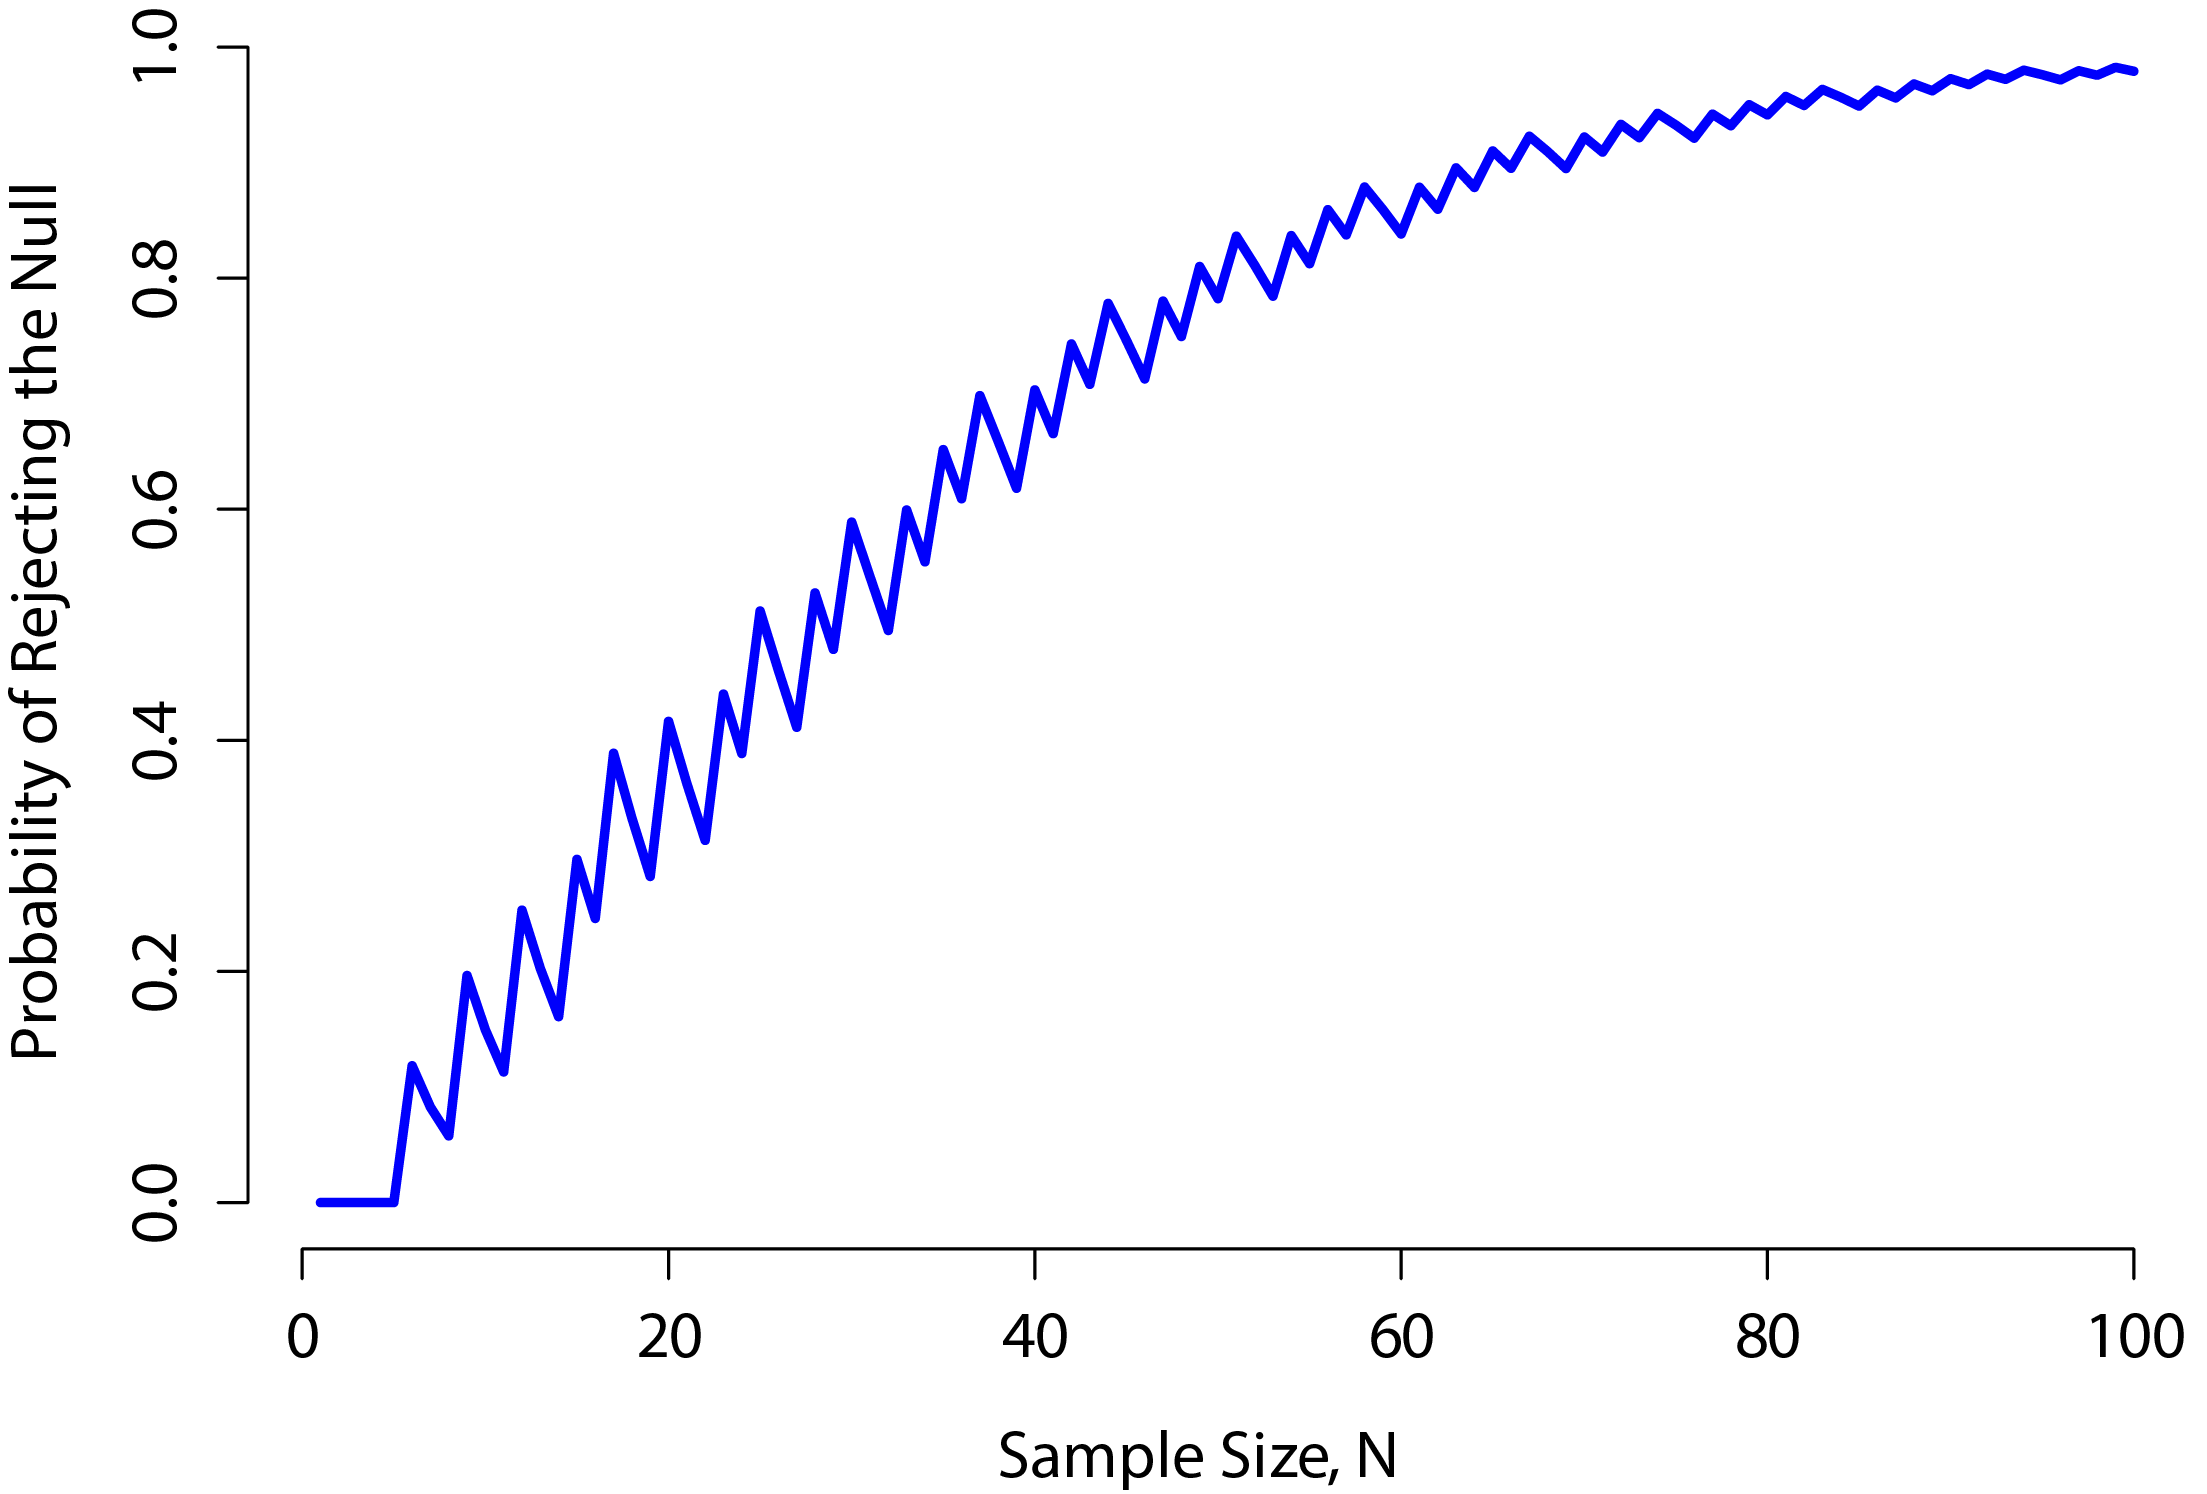
\includegraphics[width=1\linewidth]{img/nhst/powerN} 

}

\caption{The power of our test plotted as a function of the sample size $N$. In this case, the true value of $\theta$ is 0.7 but the null hypothesis is that $\theta = 0.5$. Overall, larger $N$ means greater power. (The small zig-zags in this function occur because of some odd interactions between $\theta$, $\alpha$ and the fact that the binomial distribution is discrete, it doesn't matter for any serious purpose).}\label{fig:powerfunctionsample}
\end{figure}

Because power is important, whenever you're contemplating running an experiment it would be pretty useful to know how much power you're likely to have. It's never possible to know for sure since you can't possibly know what your real effect size is. However, it's often (well, sometimes) possible to guess how big it should be. If so, you can guess what sample size you need! This idea is called {\textbf{power analysis}}, and if it's feasible to do it then it's very helpful. It can tell you something about whether you have enough time or money to be able to run the experiment successfully. It's increasingly common to see people arguing that power analysis should be a required part of experimental design, so it's worth knowing about. I don't discuss power analysis in this book, however. This is partly for a boring reason and partly for a substantive one. The boring reason is that I haven't had time to write about power analysis yet. The substantive one is that I'm still a little suspicious of power analysis. Speaking as a researcher, I have very rarely found myself in a position to be able to do one. It's either the case that (a) my experiment is a bit non-standard and I don't know how to define effect size properly, or (b) I literally have so little idea about what the effect size will be that I wouldn't know how to interpret the answers. Not only that, after extensive conversations with someone who does stats consulting for a living (my wife, as it happens), I can't help but notice that in practice the \emph{only} time anyone ever asks her for a power analysis is when she's helping someone write a grant application. In other words, the only time any scientist ever seems to want a power analysis in real life is when they're being forced to do it by bureaucratic process. It's not part of anyone's day to day work. In short, I've always been of the view that whilst power is an important concept, power \emph{analysis} is not as useful as people make it sound, except in the rare cases where (a) someone has figured out how to calculate power for your actual experimental design and (b) you have a pretty good idea what the effect size is likely to be.\footnote{One possible exception to this is when researchers study the effectiveness of a new medical treatment and they specify in advance what an important effect size would be to detect, for example over and above any existing treatment. In this way some information about the potential value of a new treatment can be obtained.} Maybe other people have had better experiences than me, but I've personally never been in a situation where both (a) and (b) were true. Maybe I'll be convinced otherwise in the future, and probably a future version of this book would include a more detailed discussion of power analysis, but for now this is about as much as I'm comfortable saying about the topic.

\hypertarget{nhstmess}{%
\section{Some issues to consider}\label{nhstmess}}

What I've described to you in this chapter is the orthodox framework for null hypothesis significance testing (NHST). Understanding how NHST works is an absolute necessity because it has been the dominant approach to inferential statistics ever since it came to prominence in the early 20th century. It's what the vast majority of working scientists rely on for their data analysis, so even if you hate it you need to know it. However, the approach is not without problems. There are a number of quirks in the framework, historical oddities in how it came to be, theoretical disputes over whether or not the framework is right, and a lot of practical traps for the unwary. I'm not going to go into a lot of detail on this topic, but I think it's worth briefly discussing a few of these issues.

\hypertarget{neyman-versus-fisher}{%
\subsection{Neyman versus Fisher}\label{neyman-versus-fisher}}

The first thing you should be aware of is that orthodox NHST is actually a mash-up of two rather different approaches to hypothesis testing, one proposed by Sir Ronald Fisher and the other proposed by Jerzy Neyman (for a historical summary \protect\hyperlink{ref-Lehmann2011}{Lehmann, 2011}). The history is messy because Fisher and Neyman were real people whose opinions changed over time, and at no point did either of them offer ``the definitive statement'' of how we should interpret their work many decades later. That said, here's a quick summary of what I take these two approaches to be.

First, let's talk about Fisher's approach. As far as I can tell, Fisher assumed that you only had the one hypothesis (the null) and that what you want to do is find out if the null hypothesis is inconsistent with the data. From his perspective, what you should do is check to see if the data are ``sufficiently unlikely'' according to the null. In fact, if you remember back to our earlier discussion, that's how Fisher defines the \(p\)-value. According to Fisher, if the null hypothesis provided a very poor account of the data then you could safely reject it. But, since you don't have any other hypotheses to compare it to, there's no way of ``accepting the alternative'' because you don't necessarily have an explicitly stated alternative. That's more or less all there is to it.

In contrast, Neyman thought that the point of hypothesis testing was as a guide to action and his approach was somewhat more formal than Fisher's. His view was that there are multiple things that you could \emph{do} (accept the null or accept the alternative) and the point of the test was to tell you which one the data support. From this perspective, it is critical to specify your alternative hypothesis properly. If you don't know what the alternative hypothesis is, then you don't know how powerful the test is, or even which action makes sense. His framework genuinely requires a competition between different hypotheses. For Neyman, the \(p\) value didn't directly measure the probability of the data (or data more extreme) under the null, it was more of an abstract description about which ``possible tests'' were telling you to accept the null, and which ``possible tests'' were telling you to accept the alternative.

As you can see, what we have today is an odd mishmash of the two. We talk about having both a null hypothesis and an alternative (Neyman), but usually\footnote{Although this book describes both Neyman's and Fisher's definition of the \(p\) value, most don't. Most introductory textbooks will only give you the Fisher version.} define the \(p\) value in terms of extreme data (Fisher), but we still have \(\alpha\) values (Neyman). Some of the statistical tests have explicitly specified alternatives (Neyman) but others are quite vague about it (Fisher). And, according to some people at least, we're not allowed to talk about accepting the alternative (Fisher). It's a mess, but I hope this at least explains why it's a mess.

\hypertarget{bayesians-versus-frequentists}{%
\subsection{Bayesians versus frequentists}\label{bayesians-versus-frequentists}}

Earlier on in this chapter I was quite emphatic about the fact that you \emph{cannot} interpret the \(p\) value as the probability that the null hypothesis is true. NHST is fundamentally a frequentist tool (see Chapter \ref{probability}) and as such it does not allow you to assign probabilities to hypotheses. The null hypothesis is either true or it is not. The Bayesian approach to statistics interprets probability as a degree of belief, so it's totally okay to say that there is a 10\% chance that the null hypothesis is true. That's just a reflection of the degree of confidence that you have in this hypothesis. You aren't allowed to do this within the frequentist approach. Remember, if you're a frequentist, a probability can only be defined in terms of what happens after a large number of independent replications (i.e., a long run frequency). If this is your interpretation of probability, talking about the ``probability'' that the null hypothesis is true is complete gibberish: a null hypothesis is either true or it is false. There's no way you can talk about a long run frequency for this statement. To talk about ``the probability of the null hypothesis'' is as meaningless as ``the colour of freedom.'' It doesn't have one!

Most importantly, this \emph{isn't} a purely ideological matter. If you decide that you are a Bayesian and that you're okay with making probability statements about hypotheses, you have to follow the Bayesian rules for calculating those probabilities. I'll talk more about this in Chapter \ref{bayes}, but for now what I want to point out to you is the \(p\) value is a \emph{terrible} approximation to the probability that \(H_0\) is true. If what you want to know is the probability of the null, then the \(p\) value is not what you're looking for!

\hypertarget{traps}{%
\subsection{Traps}\label{traps}}

As you can see, the theory behind hypothesis testing is a mess, and even now there are arguments in statistics about how it ``should'' work. However, disagreements among statisticians are not our real concern here. Our real concern is practical data analysis. And while the ``orthodox'' approach to null hypothesis significance testing has many drawbacks, even an unrepentant Bayesian like myself would agree that they can be useful if used responsibly. Most of the time they give sensible answers and you can use them to learn interesting things. Setting aside the various ideologies and historical confusions that we've discussed, the fact remains that the biggest danger in all of statistics is \emph{thoughtlessness}. I don't mean stupidity, I literally mean thoughtlessness. The rush to interpret a result without spending time thinking through what each test actually says about the data, and checking whether that's consistent with how you've interpreted it. That's where the biggest trap lies.

To give an example of this, consider the following example (see \protect\hyperlink{ref-Gelman2006}{Gelman \& Stern, 2006}). Suppose I'm running my ESP study and I've decided to analyse the data separately for the male participants and the female participants. Of the male participants, 33 out of 50 guessed the colour of the card correctly. This is a significant effect (\(p = .03\)). Of the female participants, 29 out of 50 guessed correctly. This is not a significant effect (\(p = .32\)). Upon observing this, it is extremely tempting for people to start wondering why there is a difference between males and females in terms of their psychic abilities. However, this is wrong. If you think about it, we haven't \emph{actually} run a test that explicitly compares males to females. All we have done is compare males to chance (binomial test was significant) and compared females to chance (binomial test was non significant). If we want to argue that there is a real difference between the males and the females, we should probably run a test of the null hypothesis that there is no difference! We can do that using a different hypothesis test,\footnote{In this case, the Pearson chi-square test of independence (Chapter \ref{chisquare})} but when we do that it turns out that we have no evidence that males and females are significantly different (\(p = .54\)). \emph{Now} do you think that there's anything fundamentally different between the two groups? Of course not. What's happened here is that the data from both groups (male and female) are pretty borderline. By pure chance one of them happened to end up on the magic side of the \(p = .05\) line, and the other one didn't. That doesn't actually imply that males and females are different. This mistake is so common that you should always be wary of it. The difference between significant and not-significant is \emph{not} evidence of a real difference. If you want to say that there's a difference between two groups, then you have to test for that difference!

The example above is just that, an example. I've singled it out because it's such a common one, but the bigger picture is that data analysis can be tricky to get right. Think about \emph{what} it is you want to test, \emph{why} you want to test it, and whether or not the answers that your test gives could possibly make any sense in the real world.

\hypertarget{summary-4}{%
\section{Summary}\label{summary-4}}

Null hypothesis testing is one of the most ubiquitous elements to statistical theory. The vast majority of scientific papers report the results of some hypothesis test or another. As a consequence it is almost impossible to get by in science without having at least a cursory understanding of what a \(p\)-value means, making this one of the most important chapters in the book. As usual, I'll end the chapter with a quick recap of the key ideas that we've talked about:

\begin{itemize}
\tightlist
\item
  Research hypotheses and statistical hypotheses. Null and alternative hypotheses. (Section \ref{hypotheses}).
\item
  Type 1 and Type 2 errors (Section \ref{errortypes})
\item
  Test statistics and sampling distributions (Section \ref{teststatistics})
\item
  Hypothesis testing as a decision making process (Section \ref{decisionmaking})
\item
  \(p\)-values as ``soft'' decisions (Section \ref{pvalue})
\item
  Writing up the results of a hypothesis test (Section \ref{writeup})
\item
  Running the hypothesis test in practice (Section \ref{runhyp})
\item
  Effect size and power (Section \ref{effectsize})
\item
  A few issues to consider regarding hypothesis testing (Section \ref{nhstmess})
\end{itemize}

Later in the book, in Chapter \ref{bayes}, I'll revisit the theory of null hypothesis tests from a Bayesian perspective and introduce a number of new tools that you can use if you aren't particularly fond of the orthodox approach. But for now, though, we're done with the abstract statistical theory, and we can start discussing specific data analysis tools.

\hypertarget{part-v.-statistical-tools}{%
\chapter*{Part V. Statistical Tools}\label{part-v.-statistical-tools}}
\addcontentsline{toc}{chapter}{Part V. Statistical Tools}

\hypertarget{factoranalysis}{%
\chapter{Factor Analysis}\label{factoranalysis}}

Previous chapters have covered statistical tests for differences between two or more groups. However, sometimes when conducting research, we may wish to examine how multiple variables \emph{co-vary}. That is, how they are related to each other and whether the patterns of relatedness suggest anything interesting and meaningful. For example, we are often interested in exploring whether there are any underlying unobserved {\textbf{latent factors}} that are represented by the observed, directly measured, variables in our dataset. In statistics, latent factors are initially hidden variables that are not directly observed but are rather inferred (through statistical analysis) from other variables that are observed (directly measured).

In this chapter we will consider a number of different Factor Analysis and related techniques, starting with Exploratory Factor Analysis (EFA). EFA is a statistical technique for identifying underlying latent factors in a data set (Section \ref{EFA}). Then in Section \ref{PCA} we will cover Principal Component Analysis (PCA) which is a data reduction technique which, strictly speaking, does not identify underlying latent factors. Instead, PCA simply produces a linear combination of observed variables. Following this, the Section (\ref{CFA}) on Confirmatory Factor Analysis (CFA) shows that, unlike EFA, with CFA you start with an idea - a model - of how the variables in your data are related to each other. You then test your model against the observed data and assess how good a fit the model is. A more sophisticated version of CFA is the so-called Multi-Trait Multi-Method (MTMM) approach (Section \ref{MTMM}) in which both latent factor and method variance are included in the model. This is useful when there are different methodological approaches used for measurement and therefore method variance is an important consideration. Finally, we will cover a related analysis: internal consistency reliability analysis tests how consistently a scale measures a psychological construct (Section \ref{rel}).

\hypertarget{EFA}{%
\section{Exploratory Factor Analysis}\label{EFA}}

{\textbf{Exploratory Factor Analysis (EFA)}} is a statistical technique for revealing any hidden latent factors that can be inferred from our observed data. This technique calculates to what extent a set of measured variables, for example V1, V2, V3, V4, and V5, can be represented as measures of an underlying latent factor. This latent factor cannot be measured through just one observed variable but instead is manifested in the relationships it causes in a set of observed variables.

In Figure \ref{fig:fa1} each observed variable V is `caused' to some extent by the underlying latent factor (F), depicted by the coefficients b1 to b5 (also called factor loadings). Each observed variable also has an associated error term, e1 to e5. Each error term is the variance in the associated observed variable, \(V_i\), that is unexplained by the underlying latent factor.

\begin{figure}

{\centering 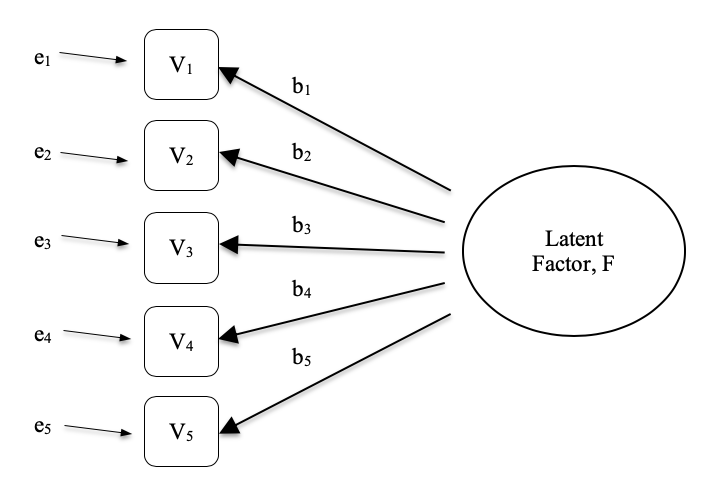
\includegraphics[width=1\linewidth]{img/factoranalysis/fa1} 

}

\caption{Latent factor underlying the relationship between several observed variables}\label{fig:fa1}
\end{figure}

In Psychology, latent factors represent psychological phenomena or constructs that are difficult to directly observe or measure. For example, personality, or intelligence, or thinking style. In the example in Figure \ref{fig:fa1} we may have asked people five specific questions about their behaviour or attitudes, and from that we are able to get a picture about a personality construct called, for example, extraversion. A different set of specific questions may give us a picture about an individual's introversion, or their conscientiousness.

Here's another example: we may not be able to directly measure statistics anxiety, but we can measure whether statistics anxiety is high or low with a set of questions in a questionnaire. For example, ``Q1: Doing the assignment for a statistics course,'' ``Q2: Trying to understand the statistics described in a journal article,'' and ``Q3: Asking the lecturer for help in understanding something from the course,'' etc., each rated from low anxiety to high anxiety. People with high statistics anxiety will tend to give similarly high responses on these observed variables because of their high statistics anxiety. Likewise, people with low statistics anxiety will give similar low responses to these variables because of their low statistics anxiety.

In exploratory factor analysis (EFA), we are essentially exploring the correlations between observed variables to uncover any interesting, important underlying (latent) factors that are identified when observed variables co-vary. We can use statistical software to estimate any latent factors and to identify which of our variables have a high loading\footnote{Quite helpfully, factor loadings can be interpreted like standardized regression coefficients} (e.g.~loading \(>0.5\)) on each factor, suggesting they are a useful measure, or indicator, of the latent factor. Part of this process includes a step called rotation, which to be honest is a pretty weird idea but luckily we don't have to worry about understanding it; we just need to know that it is helpful because it makes the pattern of loadings on different factors much clearer. As such, rotation helps with seeing more clearly which variables are linked substantively to each factor. We also need to decide how many factors are reasonable given our data, and helpful in this regard is something called Eigen values. We'll come back to this in a moment, after we have covered some of the main assumptions of EFA.

\hypertarget{checking-assumptions}{%
\subsection{Checking assumptions}\label{checking-assumptions}}

There are a couple of assumptions that need to be checked as part of the analysis. The first assumption is {\textbf{sphericity}}, which essentially checks that the variables in your dataset are correlated with each other to the extent that they can potentially be summarised with a smaller set of factors. Bartlett's test for sphericity checks whether the observed correlation matrix diverges significantly from a zero (or null) correlation matrix. So, if Bartlett's test is significant (\(p<.05\)), this indicates that the observed correlation matrix is significantly divergent from the null, and is therefore suitable for EFA.

The second assumption is {\textbf{sampling adequacy}} and is checked using the Kaiser-Meyer-Olkin (KMO) Measure of Sampling Adequacy (MSA). The KMO index is a measure of the proportion of variance among observed variables that might be common variance. Using partial correlations, it checks for factors that load just two items. We seldom, if ever, want EFA producing a lot of factors loading just two items each. KMO is about sampling adequacy because partial correlations are typically seen with inadequate samples. If the KMO index is high (\(\approx\) 1), the EFA is efficient whereas if KMO is low (\(\approx\) 0), the EFA is not relevant. KMO values smaller than 0.5 indicates that EFA is not suitable and a KMO value of 0.6 should be present before EFA is considered suitable. Values between 0.5 and 0.7 are considered adequate, values between 0.7 and 0.9 are good and values between 0.9 and 1.0 are excellent.

\hypertarget{what-is-efa-good-for}{%
\subsection{What is EFA good for?}\label{what-is-efa-good-for}}

If the EFA has provided a good solution (i.e.~factor model), then we need to decide what to do with our shiny new factors. Researchers often use EFA during psychometric scale development. They will develop a pool of questionnaire items that they think relate to one or more psychological constructs, use EFA to see which items ``go together'' as latent factors, and then they will assess whether some items should be removed because they don't usefully or distinctly measure one of the latent factors.

In line with this approach, another consequence of EFA is to combine the variables that load onto distinct factors into a factor score, sometimes known as a scale score. There are two options for combining variables into a scale score:

\begin{itemize}
\tightlist
\item
  Create a new variable with a score weighted by the factor loadings for each item that contributes to the factor.
\item
  Create a new variable based on each item that contributes to the factor, but weighting them equally.
\end{itemize}

In the first option each item's contribution to the combined score depends on how strongly it relates to the factor. In the second option we typically just average across all the items that contribute substantively to a factor to create the combined scale score variable. Which to choose is a matter of preference, though a disadvantage with the first option is that loadings can vary quite a bit from sample to sample, and in behavioural and health sciences we are often interested in developing and using composite questionnaire scale scores across different studies and different samples. In which case it is reasonable to use a composite measure that is based on the substantive items contributing equally rather than weighting by sample specific loadings from a different sample. In any case, understanding a combined variable measure as an average of items is simpler and more intuitive than using a sample specific optimally-weighted combination.

A more advanced statistical technique, one which is beyond the scope of this book, undertakes regression modelling where latent factors are used in prediction models of other latent factors. This is called ``structural equation modelling'' and there are specific software programmes and R packages dedicated to this approach. But let's not get ahead of ourselves; what we should really focus on now is how to do an EFA in jamovi.

\hypertarget{efa-in-jamovi}{%
\subsection{EFA in jamovi}\label{efa-in-jamovi}}

First, we need some data. Twenty-five personality self-report items (see Figure \ref{fig:fa2}) taken from the International Personality Item Pool (\url{http://ipip.ori.org}) were included as part of the Synthetic Aperture Personality Assessment (SAPA) web-based personality assessment (SAPA: \url{http://sapa-project.org}) project. The 25 items are organized by five putative factors: Agreeableness, Conscientiousness, Extraversion, Neuroticism, and Openness.

\textbackslash begin\{figure\}

\{\centering 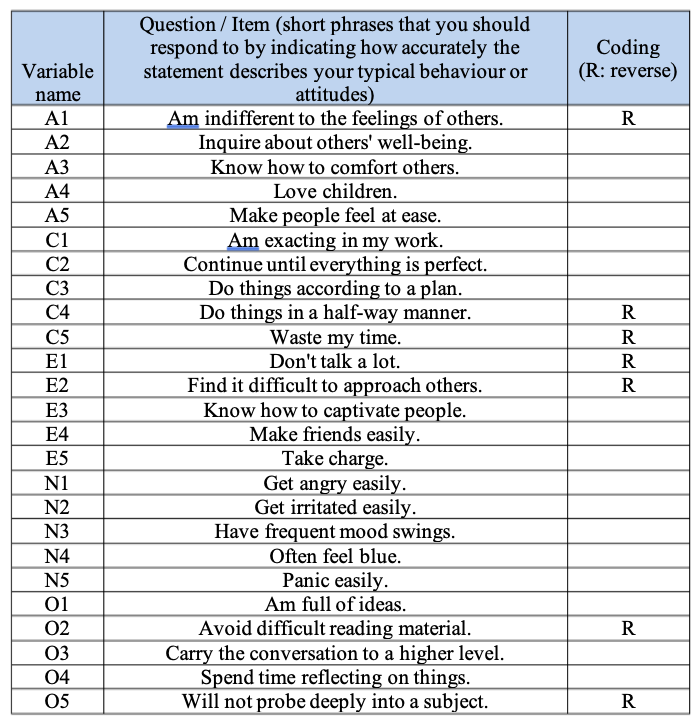
\includegraphics[width=1\linewidth]{img/factoranalysis/fa2}

\}

\textbackslash caption\{Twenty-five observed variable items organised by five putative personality factors in the dataset \textbf{\texttt{bfi\_sample.csv}}\}\label{fig:fa2}
\textbackslash end\{figure\}

The item data were collected using a 6-point response scale:

\begin{enumerate}
\def\labelenumi{\arabic{enumi}.}
\tightlist
\item
  Very Inaccurate
\item
  Moderately Inaccurate
\item
  Slightly Inaccurate
\item
  Slightly Accurate
\item
  Moderately Accurate
\item
  Very Accurate.
\end{enumerate}

A sample of N=250 responses is contained in the dataset \textbf{\texttt{bfi\_sample.csv}}. As researchers, we are interested in exploring the data to see whether there are some underlying latent factors that are measured reasonably well by the 25 observed variables in the \textbf{\texttt{bfi\_sample.csv}} data file. Open up the dataset and check that the 25 variables are coded as continuous variables (technically they are ordinal though for EFA in jamovi it mostly doesn't matter, except if you decide to calculate weighted factor scores in which case continuous variables are needed). To perform EFA in jamovi:

\begin{itemize}
\tightlist
\item
  Select `Factor - Exploratory Factor Analysis' from the main jamovi button bar to open the EFA analysis window (Figure \ref{fig:fa3}).
\item
  Select the 25 personality questions and transfer them into the `Variables' box.
\item
  Check appropriate options, including `Assumption Checks,' but also Rotation `Method,' `Number of Factors' to extract, and `Additional Output' options. See Figure \ref{fig:fa3} for suggested options for this illustrative EFA, and please note that the Rotation `Method' and `Number of Factors' extracted is typically adjusted by the researcher during the analysis to find the best result, as described below.
\end{itemize}

\begin{figure}

{\centering 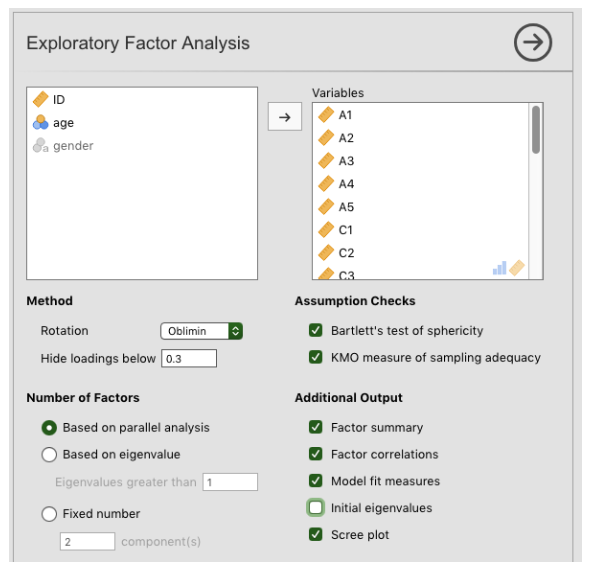
\includegraphics[width=1\linewidth]{img/factoranalysis/fa3} 

}

\caption{The jamovi EFA analysis window}\label{fig:fa3}
\end{figure}

\begin{figure}
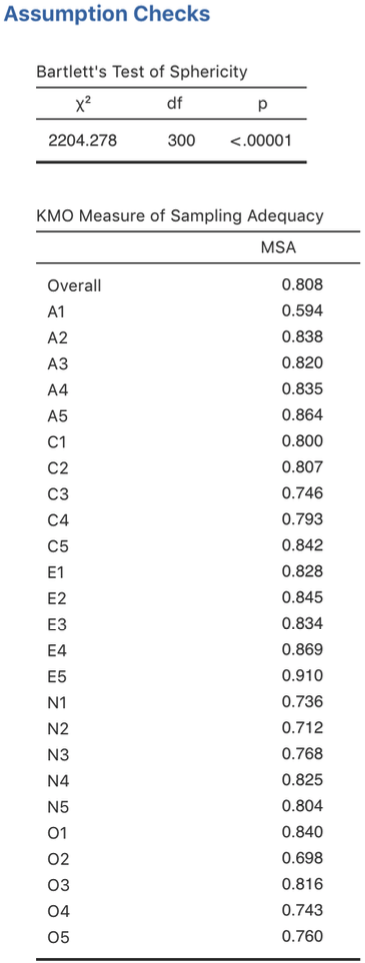
\includegraphics[width=1\linewidth]{img/factoranalysis/fa4} \caption{jamovi EFA assumption checks for the personality questionnaire data}\label{fig:fa4}
\end{figure}

First, check the assumptions (Figure \ref{fig:fa4}). You can see that (1) Bartlett's test of sphericity is significant, so this assumption is satisfied; and (2) the KMO measure of sampling adequacy (MSA) is 0.81 overall, suggesting good sampling adequacy. No problems here then!

The next thing to check is how many factors to use (or ``extract'' from the data). Three different approaches are available:

\begin{itemize}
\tightlist
\item
  One convention is to choose all components with Eigen values greater than 1\footnote{An Eigen value indicates how much of the variance in the observed variables a factor accounts for. A factor with an Eigen value \(>1\) accounts for more variance than a single observed variable}. This would give us four factors with our data (try it and see).
\item
  Examination of the scree plot, as in Figure \ref{fig:fa5}, lets you identify the ``point of inflection.'' This is the point at which the slope of the scree curve clearly levels off, below the ``elbow.'' This would give us five factors with our data. Interpreting scree plots is a bit of an art: in Figure \ref{fig:fa5} there is a noticeable step from 5 to 6 factors, but in other scree plots you look at it will not be so clear cut.
\item
  Using a parallel analysis technique, the obtained Eigen values are compared to those that would be obtained from random data. The number of factors extracted is the number with Eigen values greater than what would be found with random data.
\end{itemize}

\begin{figure}

{\centering 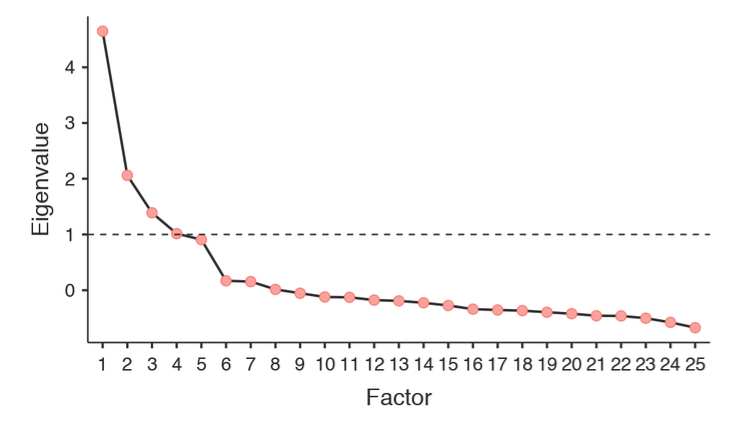
\includegraphics[width=1\linewidth]{img/factoranalysis/fa5} 

}

\caption{Scree plot of the personality data in jamovi EFA, showing a noticeable inflection and levelling off after point 5 (the "elbow")}\label{fig:fa5}
\end{figure}

\begin{figure}

{\centering 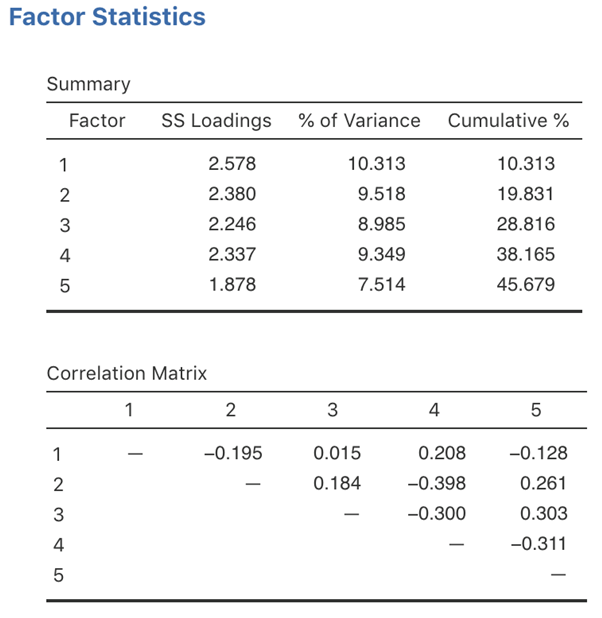
\includegraphics[width=1\linewidth]{img/factoranalysis/fa6} 

}

\caption{Factor summary statistics and correlations for a five factor solution in jamovi EFA}\label{fig:fa6}
\end{figure}

The third approach is a good one according to \protect\hyperlink{ref-Fabrigar1999}{Fabrigar et al.} (\protect\hyperlink{ref-Fabrigar1999}{1999}), although in practice researchers tend to look at all three and then make a judgement about the number of factors that are most easily or helpfully interpreted. This can be understood as the ``meaningfulness criterion,'' and researchers will typically examine, in addition to the solution from one of the approaches above, solutions with one or two more or fewer factors. They then adopt the solution which makes the most sense to them.

At the same time, we should also consider the best way to rotate the final solution. There are two main approaches to rotation: orthogonal (e.g.~`varimax') rotation forces the selected factors to be uncorrelated, whereas oblique (e.g.~`oblimin') rotation allows the selected factors to be correlated. Dimensions of interest to psychologists and behavioural scientists are not often dimensions we would expect to be orthogonal, so oblique solutions are arguably more sensible\footnote{Oblique rotations provide two factor matrices, one called a structure matrix and one called a pattern matrix. In jamovi just the pattern matrix is shown in the results as this is typically the most useful for interpretation, though some experts suggest that both can be helpful. In a structure matrix coefficients show the relationship between the variable and the factors whilst ignoring the relationship of that factor with all the other factors (i.e.~a zero-order correlation). Pattern matrix coefficients show the unique contribution of a factor to a variable whilst controlling for the effects of other factors on that variable (akin to standardized partial regression coefficient). Under orthogonal rotation, structure and pattern coefficients are the same.}

Practically, if in an oblique rotation the factors are found to be substantially correlated (positive or negative, and \(>0.3\)), as in Figure \ref{fig:fa6} where a correlation between two of the extracted factors is \(-0.398\), then this would confirm our intuition to prefer oblique rotation. If the factors are, in fact, correlated, then an oblique rotation will produce a better estimate of the true factors and a better simple structure than will an orthogonal rotation. And, if the oblique rotation indicates that the factors have close to zero correlations between one another, then the researcher can go ahead and conduct an orthogonal rotation (which should then give about the same solution as the oblique rotation).

On checking the correlation between the extracted factors at least one correlation was greater than 0.3 (Figure \ref{fig:fa6}), so an oblique (`oblimin') rotation of the five extracted factors is preferred. We can also see in Figure @ref(fig:fa6\} that the proportion of overall variance in the data that is accounted for by the five factors is 46\%. Factor one accounts for around 10\% of the variance, factors two to four around 9\% each, and factor five just over 7\%. This isn't great; it would have been better if the overall solution accounted for a more substantive proportion of the variance in our data.

Be aware that in every EFA you could potentially have the same number of factors as observed variables, but every additional factor you include will add a smaller amount of explained variance. If the first few factors explain a good amount of the variance in the original 25 variables, then those factors are clearly a useful, simpler substitute for the 25 variables. You can drop the rest without losing too much of the original variability. But if it takes 18 factors (for example) to explain most of the variance in those 25 variables, you might as well just use the original 25.

Figure \ref{fig:fa7} shows the factor loadings. That is, how the 25 different personality items load onto each of the five selected factors. We have hidden loadings less than 0.3 (set in the options shown in Figure \ref{fig:fa3}).

For Factors 1, 2, 3 and 4 the pattern of factor loadings closely matches the putative factors specified in Figure \ref{fig:fa2}. Phew! And factor 5 is pretty close, with four of the five observed variables that putatively measure ``openness'' loading pretty well onto the factor. Variable 04 doesn't quite seem to fit though, as the factor solution in Figure \ref{fig:fa7} suggests that it loads onto factor 3 (albeit with a relatively low loading) but not substantively onto factor 5.

The other thing to note is that those variables that were denoted as ``R: reverse coding'' in Figure \ref{fig:fa2} are those that have negative factor loadings. Take a look at the items A1 (``Am indifferent to the feelings of others'') and A2 (``Inquire about others' well-being''). We can see that a high score on A1 indicates low Agreeableness, whereas a high score on A2 (and all the other ``A'' variables for that matter) indicates high Agreeableness. Therefore A1 will be negatively correlated with the other ``A'' variables, and this is why it has a negative factor loading, as shown in Figure \ref{fig:fa7}.

\begin{figure}

{\centering 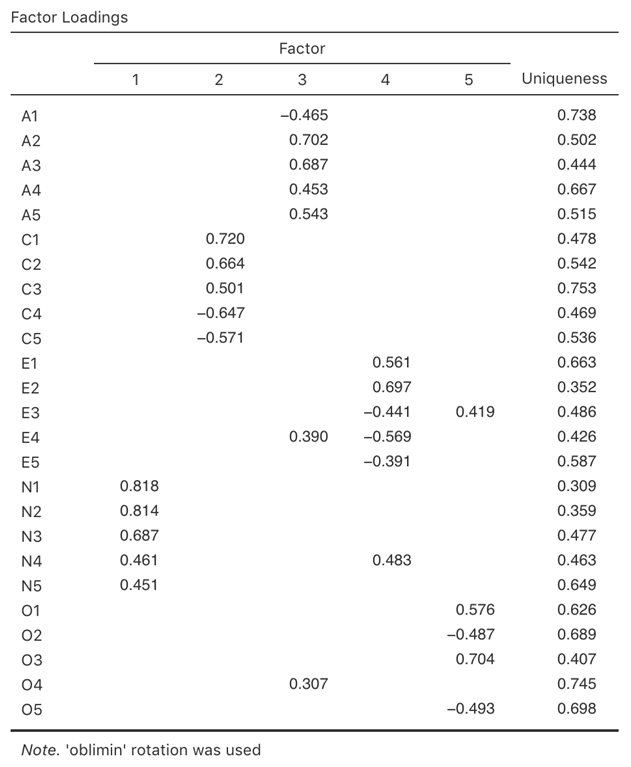
\includegraphics[width=1\linewidth]{img/factoranalysis/fa7} 

}

\caption{Factor loadings for a five factor solution in jamovi EFA}\label{fig:fa7}
\end{figure}

We can also see in Figure \ref{fig:fa7} the ``uniqueness'' of each variable. Uniqueness is the proportion of variance that is `unique' to the variable and not explained by the factors\footnote{Sometimes reported in factor analysis is ``communality'' which is the amount of variance in a variable that is accounted for by the factor solution. Uniqueness is equal to (\(1-communality\))}. For example, 74\% of the variance in `A1' is not explained by the factors in the five factor solution. In contrast, `N1' has relatively low variance not accounted for by the factor solution (31\%). Note that the greater the `uniqueness,' the lower the relevance or contribution of the variable in the factor model.

To be honest, it's unusual to get such a neat solution in EFA. It's typically quite a bit more messy than this, and often interpreting the meaning of the factors is more challenging. It's not often that you have such a clearly delineated item pool. More often you will have a whole heap of observed variables that you think may be indicators of a few underlying latent factors, but you don't have such a strong sense of which variables are going to go where!

So, we seem to have a pretty good five factor solution, albeit accounting for a relatively low overall proportion of the observed variance. Let's assume we are happy with this solution and want to use our factors in further analysis. The straightforward option is to calculate an overall (average) score for each factor by adding together the score for each variable that loads substantively onto the factor and then dividing by the number of variables. For each person in our dataset that would mean, for example for the Agreeableness factor, adding together A1 + A2 + A3 + A4 + A5, and then dividing by 5\footnote{remembering to first reverse score some variables if necessary}. In essence, this means that the factor score we have calculated is based on equally weighted scores from each of the included variables. We can do this in jamovi in two steps:

\begin{itemize}
\tightlist
\item
  Recode A1 into ``A1R'' by reverse scoring the values in the variable (i.e.~\(6=1; 5=2; 4=3; 3=4; 2=5; 1=6\)) using the jamovi transform variable command (see Figure \ref{fig:fa8}).
\item
  Compute a new variable, called ``Agreeableness', by calculating the mean of A1R, A2, A3, A4 and A5. Do this using the jamovi compute new variable command (see Figure \ref{fig:fa9}).
\end{itemize}

\begin{figure}

{\centering 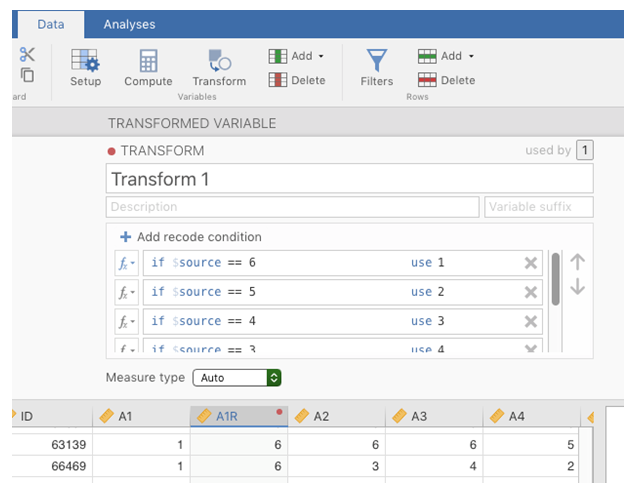
\includegraphics[width=1\linewidth]{img/factoranalysis/fa8} 

}

\caption{Recode variable using the jamovi Transform command}\label{fig:fa8}
\end{figure}

\begin{figure}

{\centering 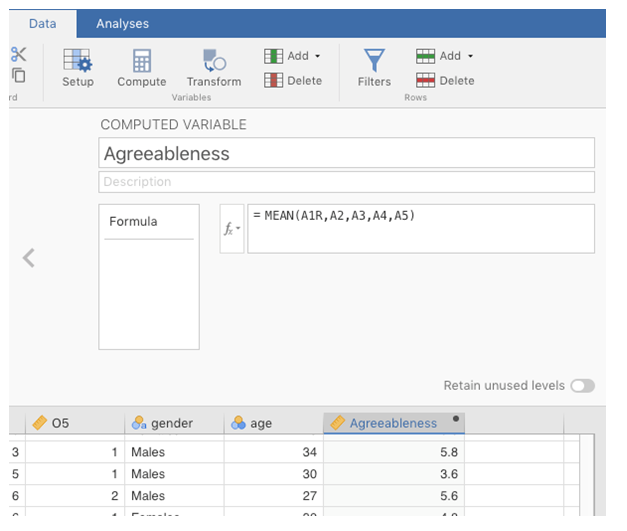
\includegraphics[width=1\linewidth]{img/factoranalysis/fa9} 

}

\caption{Compute new scale score variable using the jamovi Computed variable command}\label{fig:fa9}
\end{figure}

Another option is to create an optimally-weighted factor score index. We can use the jamovi \texttt{Rj} editor to do this in \texttt{R}. Again, there are two steps:

\begin{itemize}
\tightlist
\item
  Use the \texttt{Rj} editor to run the EFA in \texttt{R} to the same specification as the one in jamovi (i.e.~five factors and oblimin rotation) and compute optimally weighted factor scores. Save the new dataset, with the factor scores, to a file. See Figure \ref{fig:fa10}.
\item
  Open up the new file in jamovi and check that variable types have been set correctly. Label the new factor score variables corresponding to the relevant factor names or definitions (NB it is possible that the factors will not be in the expected order, so make sure you check).
\end{itemize}

\begin{figure}

{\centering 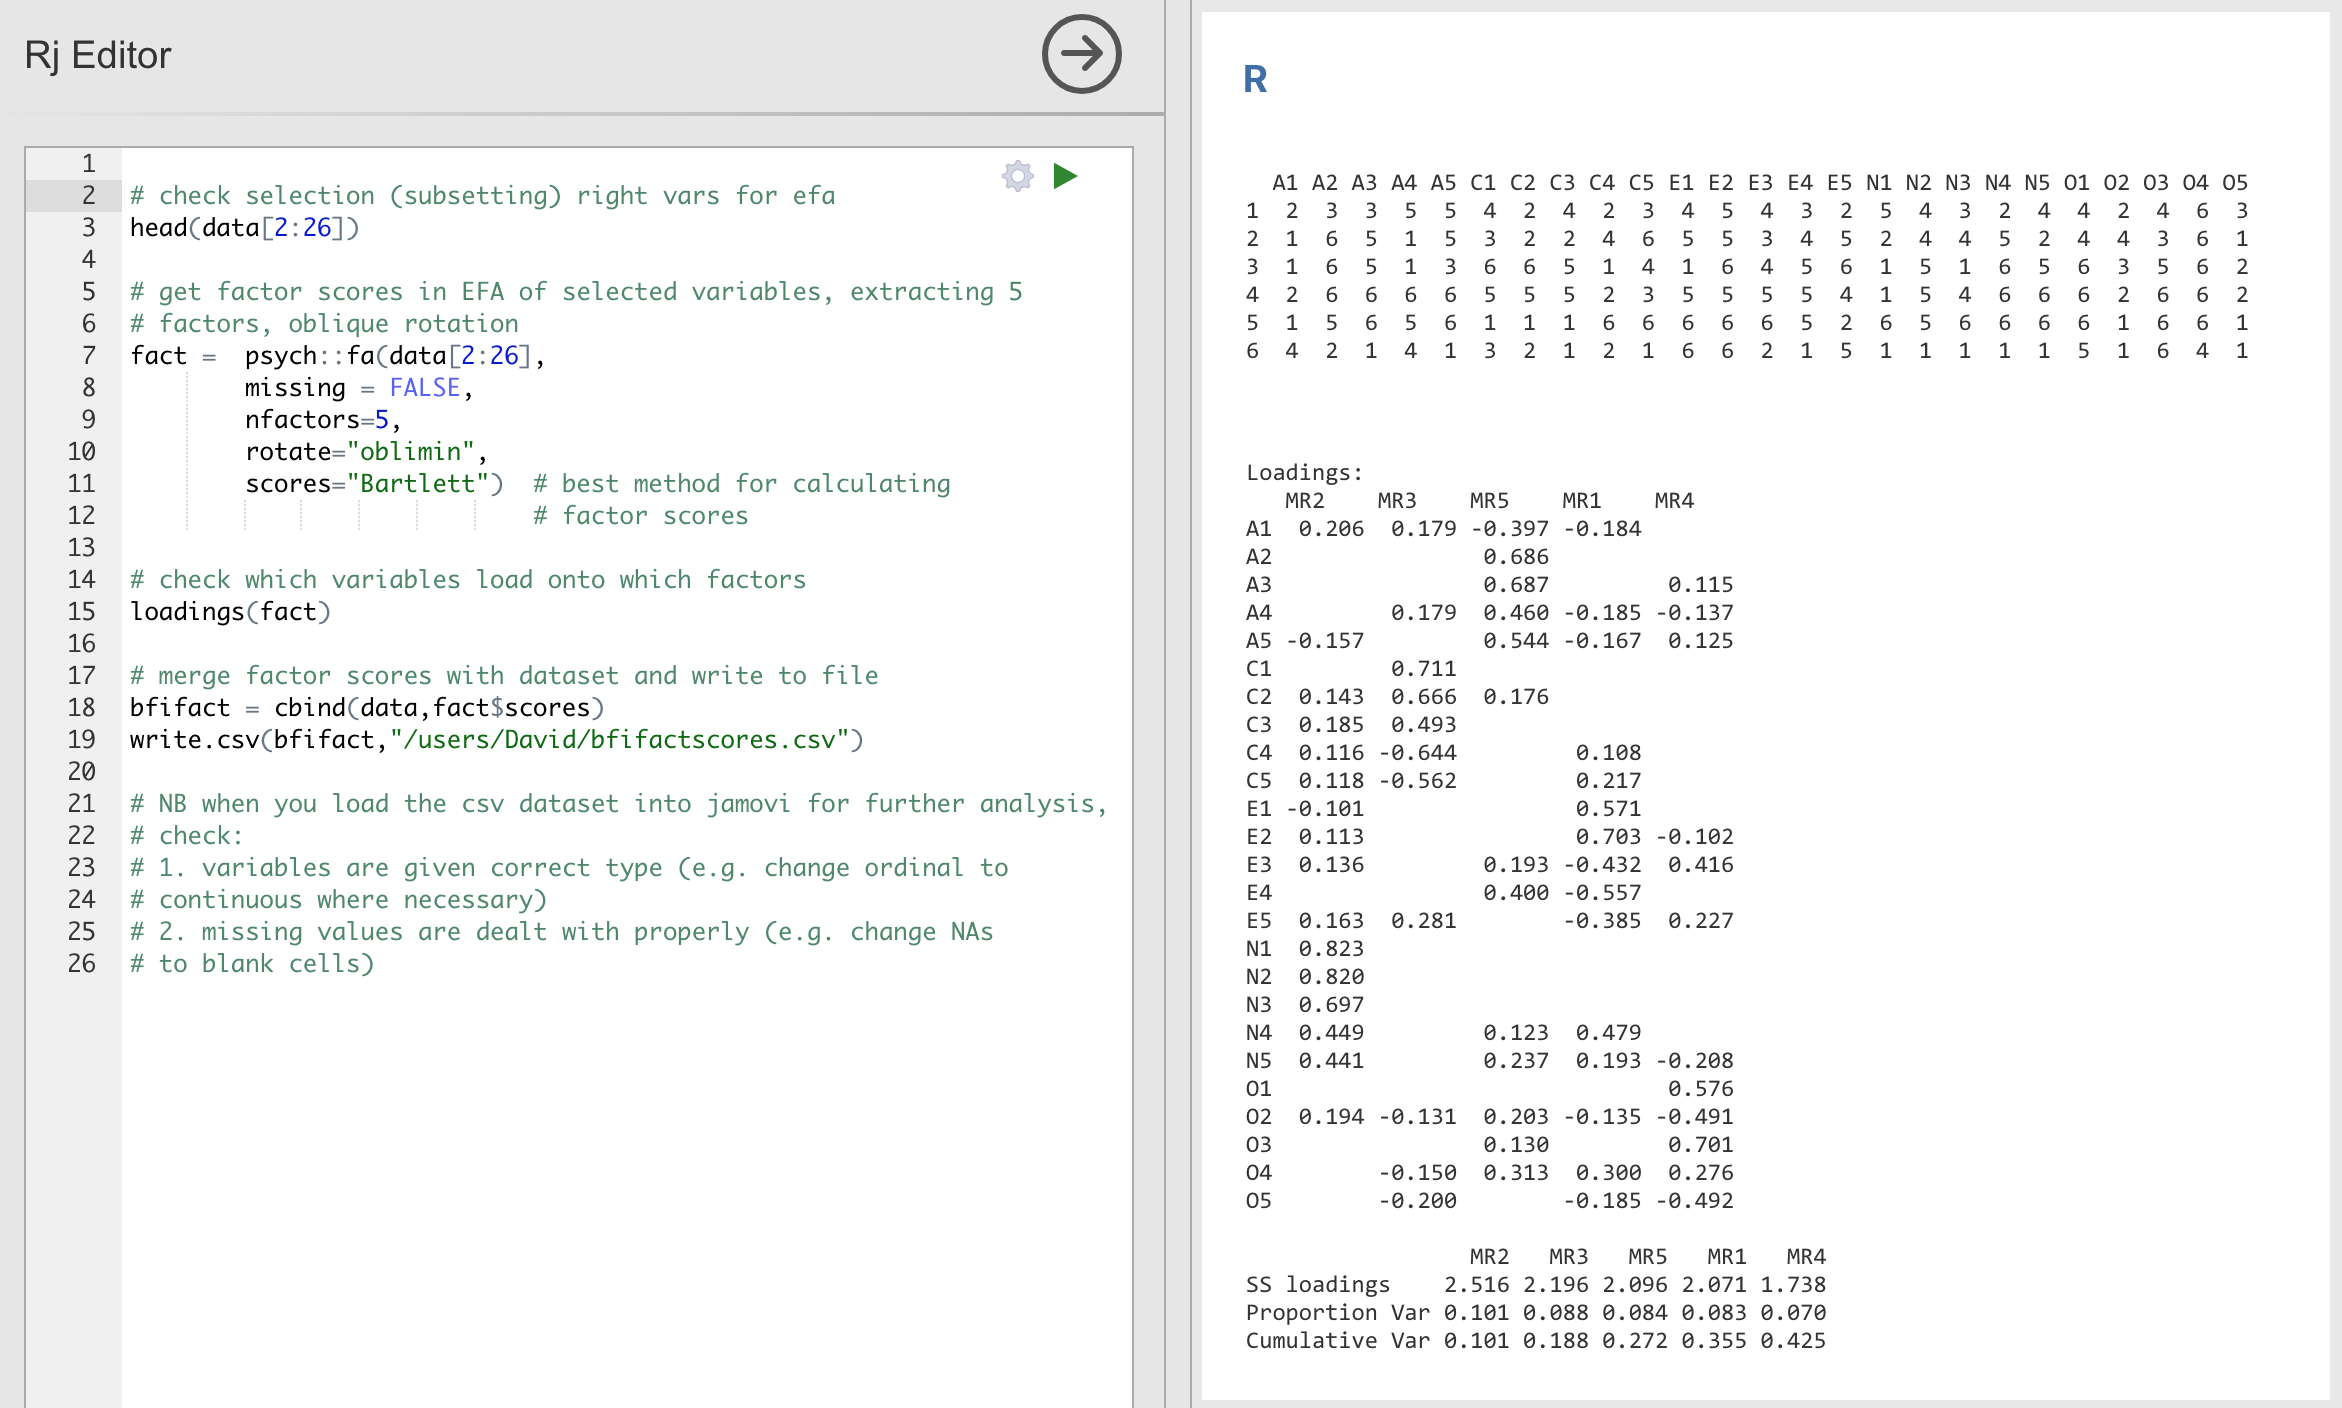
\includegraphics[width=1\linewidth]{img/factoranalysis/fa10} 

}

\caption{`Rj` editor commands for creating optimally weighted factor scores for the five factor solution}\label{fig:fa10}
\end{figure}

\begin{figure}

{\centering 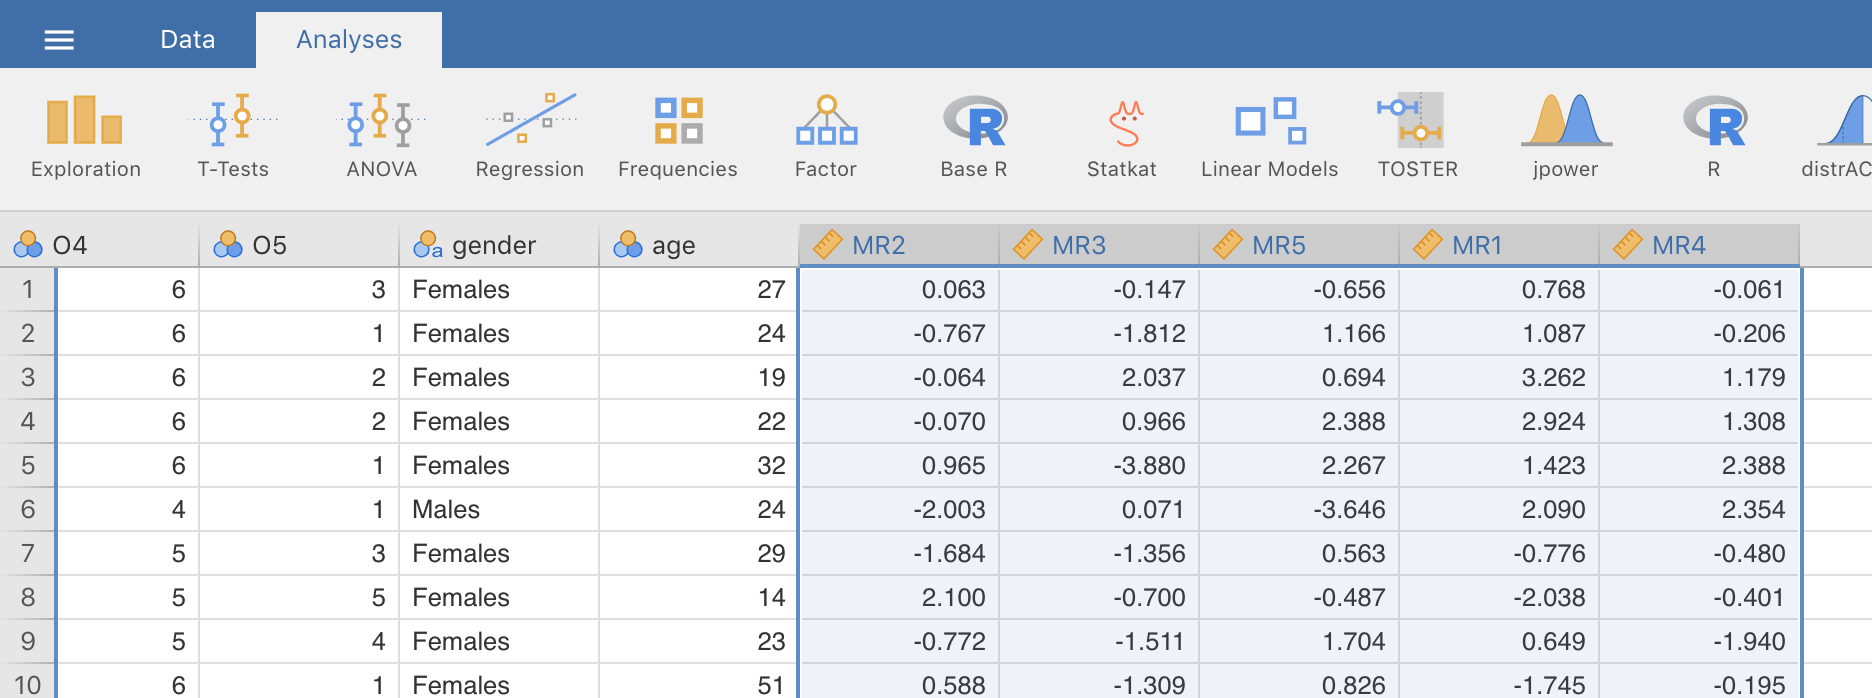
\includegraphics[width=1\linewidth]{img/factoranalysis/fa11} 

}

\caption{The newly created data file “bfifactscores.csv” created in the `Rj` editor and containing the five factor score variables. Note that each of the new factor score variables is labelled corresponding to the order that the factors are listed in the factor loadings table}\label{fig:fa11}
\end{figure}

Now you can go ahead and undertake further analyses, using either the factor-based scores (a mean scale score approach) or using the optimally-weighted factor scores calculated via the **`Rj\} editor. Your choice! For example, one thing you might like to do is see whether there are any gender differences in each of our personality scales. We did this for the Agreeableness score that we calculated using the factor-based score approach, and although the plot (Figure \ref{fig:fa12}) showed that males were less agreeable than females, this was not a significant difference (Man-Whitney \(U=5760.5, p=.073\)).

\begin{figure}

{\centering 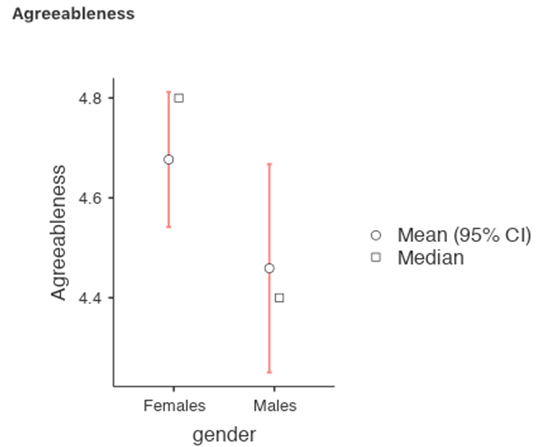
\includegraphics[width=1\linewidth]{img/factoranalysis/fa12} 

}

\caption{Comparing differences in Agreeableness factor-based scores between males and females}\label{fig:fa12}
\end{figure}

\hypertarget{writing-up-an-efa}{%
\subsection{Writing up an EFA}\label{writing-up-an-efa}}

Hopefully, so far we have given you some sense of EFA and how to undertake EFA in jamovi. So, once you have completed your EFA, how do you write it up? There is not a formal standard way to write up an EFA, and examples tend to vary by discipline and researcher. That said, there are some fairly standard pieces of information to include in your write-up:

\begin{itemize}
\tightlist
\item
  What are the theoretical underpinnings for the area you are studying, and specifically for the constructs that you are interested in uncovering through EFA.
\item
  A description of the sample (e.g.~demographic information, sample size, sampling method).
\item
  A description of the type of data used (e.g., nominal, continuous) and descriptive statistics.
\item
  Describe how you went about testing the assumptions for EFA. Details regarding sphericity checks and measures of sampling adequacy should be reported.
\item
  Explain what FA extraction method (e.g.~maximum likelihood) was used.
\item
  Explain the criteria and process used for deciding how many factors were extracted in the final solution, and which items were selected. Clearly explain the rationale for key decisions during the EFA process.
\item
  Explain what rotation methods were attempted, the reasons why, and the results.
\item
  Final factor loadings should be reported in the results, in a table. This table should also report the uniqueness (or communality) for each variable (in the final column). Factor loadings should be reported with descriptive labels in addition to item numbers. Correlations between the factors should also be included, either at the bottom of this table, in a separate table.
\item
  Meaningful names for the extracted factors should be provided. You may like to use previously selected factor names, but on examining the actual items and factors you may think a different name is more appropriate
\end{itemize}

\hypertarget{PCA}{%
\section{Principal Component Analysis}\label{PCA}}

In the previous section we saw that EFA works to identify underlying latent factors. And, as we saw, in one scenario the smaller number of latent factors can be used in further statistical analysis using some sort of combined factor scores.

In this way EFA is being used as a ``data reduction'' technique. Another type of data reduction technique, sometimes seen as part of the EFA family, is {\textbf{principal component analysis (PCA)}}. However, PCA does not identify underlying latent factors. Instead it creates a linear composite score from a larger set of measured variables.

PCA simply produces a mathematical transformation to the original data with no assumptions about how the variables co-vary. The aim of PCA is to calculate a few linear combinations (components) of the original variables that can be used to summarize the observed data set without losing much information. However, if identification of underlying structure is a goal of the analysis, then EFA is to be preferred. And, as we saw, EFA produces factor scores that can be used for data reduction purposes just like principal component scores (\protect\hyperlink{ref-Fabrigar1999}{Fabrigar et al., 1999}).

PCA has been popular in Psychology for a number of reasons, and therefore it's worth covering, although nowadays EFA is just as easy to do given the power of desktop computers and can be less susceptible to bias than PCA, especially with a small number of factors and variables. We'll use the same \textbf{\texttt{bfi\_sample.csv}} data as before. Much of the procedure is similar to EFA, so although there are some conceptual differences, practically the steps are the same\footnote{\ldots and that means there is a fair bit of repetition in the PCA steps set out in the next section. Sorry about that, but hopefully it is not too bad!}, and with large samples and a sufficient number of factors and variables, the results from PCA and EFA should be fairly similar.

\hypertarget{performing-pca-in-jamovi}{%
\subsection{Performing PCA in jamovi}\label{performing-pca-in-jamovi}}

Once you have loaded up the \textbf{\texttt{bfi\_sample.csv}} data, select `Factor - Principal Component Analysis' from the main jamovi button bar to open the PCA analysis window (Figure \ref{fig:pca1}). Then select the 25 personality questions and transfer them into the `Variables' box. Check appropriate options, including `Assumption Checks,' but also Rotation `Method,' `Number of Factors to extract, and `Additional Output' options. See Figure \ref{fig:pca1} for suggested options for this PCA, and please note that the Rotation `Method' and `Number of Factors' extracted is typically adjusted during the analysis to find the best result, as described below.

\begin{figure}

{\centering 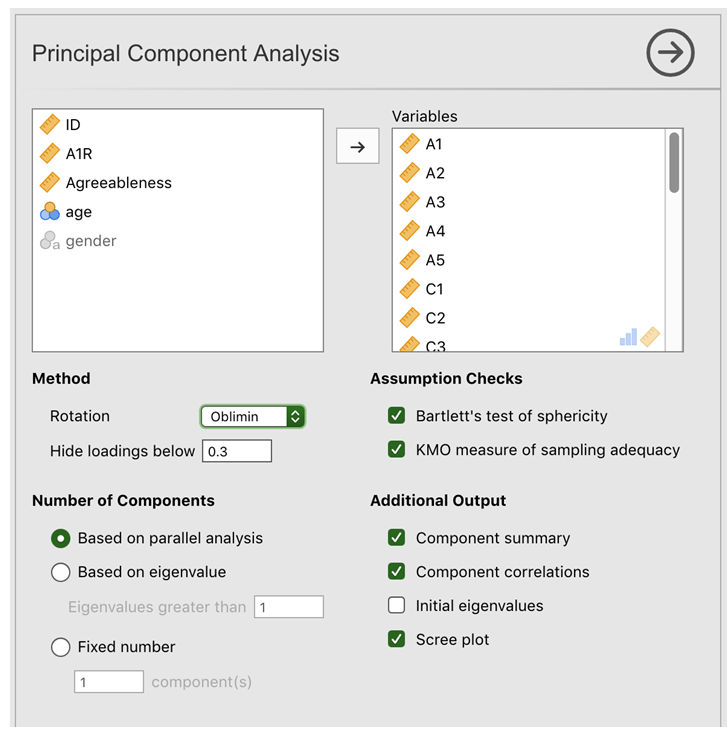
\includegraphics[width=1\linewidth]{img/factoranalysis/pca1} 

}

\caption{The jamovi PCA analysis window}\label{fig:pca1}
\end{figure}

First, checking the assumptions, you can see that (1) Bartlett's test of sphericity is significant, so this assumption is satisfied; and (2) the KMO measure of sampling adequacy (MSA) is 0.81 overall, suggesting very good sampling adequacy. No problems here then!

\begin{figure}

{\centering \includegraphics[width=1\linewidth]{img/factoranalysis/pca2} 

}

\caption{jamovi PCA assumption checks for the personality item data}\label{fig:pca2}
\end{figure}

The next thing to check is how many components to use (or ``extract'' from the data). As with EFA, three different approaches are available:

\begin{itemize}
\tightlist
\item
  One convention is to choose all components with Eigen values greater than 1. This would give us two components with our data.
\item
  Examination of the scree plot, as in Figure \ref{fig:pca3}, lets you identify the ``point of inflection.'' This is the point at which the slope of the scree curve clearly levels off, below the ``elbow.'' Again, this would give us two components as the levelling off clearly occurs after the second component.
\item
  Using a parallel analysis technique, the obtained Eigen values are compared to those that would be obtained from random data. The number of components extracted is the number with Eigen values greater than what would be found with random data.
\end{itemize}

The third approach is a good one according to (\protect\hyperlink{ref-Fabrigar1999}{Fabrigar et al., 1999}), although in practice researchers tend to look at all three and then make a judgement about the number of components that are most easily or helpfully interpreted. This can be understood as the ``meaningfulness criterion,'' and researchers will typically examine, in addition to the solution from one of the approaches above, solutions with one or two more or fewer components. They then adopt the solution which makes the most sense to them.

\begin{figure}

{\centering \includegraphics[width=1\linewidth]{img/factoranalysis/pca3} 

}

\caption{Scree plot of the personality item data in jamovi PCA, showing the levelling off point, the “elbow”, after component 5}\label{fig:pca3}
\end{figure}

At the same time, we should also consider the best way to rotate the final solution. Again, as with EFA, there are two main approaches to rotation: orthogonal (e.g.~``varimax'') rotation forces the selected components to be uncorrelated; whereas oblique (e.g.~``oblimin'') rotation allows the selected components to be correlated. Dimensions of interest to psychologists and behavioural scientists are not often dimensions we would expect to be orthogonal, so oblique solutions are arguably more sensible. Practically, if in an oblique rotation the components are found to be substantially correlated (i.e.~\(>0.3\)) then this would confirm our intuition to prefer oblique rotation. If the components are, in fact, correlated, then an oblique rotation will produce a better estimate of the true components and a better simple structure than will an orthogonal rotation. And, if the oblique rotation indicates that the components have close to zero correlations between one another, then the researcher can go ahead and conduct an orthogonal rotation (which should then give about the same solution as the oblique rotation). In Figure \ref{fig:pca4} we see that none of the correlations is \(>0.3\) so it is appropriate to switch to orthogonal (varimax) rotation.

\begin{figure}

{\centering \includegraphics[width=1\linewidth]{img/factoranalysis/pca4} 

}

\caption{Component summary statistics and correlations for a five component solution in jamovi PCA}\label{fig:pca4}
\end{figure}

In Figure \ref{fig:pca4} we also have the proportion of overall variance in the data that is accounted for by the two components. Components one and two account for just over 12\% of the variance each. Taken together, the five component solution accounts for just over half of the variance (56\%) in the observed data. Be aware that in every PCA you could potentially have the same number of components as observed variables, but every additional component you include will add a smaller amount of explained variance. If the first few components explain a good amount of the variance in the original 25 variables, then those components are clearly a useful, simpler substitute for all 25 variables. You can drop the rest without losing too much of the original variability. But if it takes 18 components to explain most of the variance in those 25 variables, you might as well just use the original 25.

\begin{figure}

{\centering \includegraphics[width=1\linewidth]{img/factoranalysis/pca5} 

}

\caption{Component loadings for a five component solution in jamovi PCA}\label{fig:pca5}
\end{figure}

Figure \ref{fig:pca5} shows the component loadings. That's is, how the 25 different personality items load onto each of the selected components. We have hidden loadings less than 0.4 (set in the options shown in Figure \ref{fig:pca1}) as we were interested in items with a substantive loading and setting the threshold at the higher 0.4 value also provided a cleaner, clearer solution.

For components 1, 2, 3 and 4 the pattern of component loadings closely matches the putative factors specified in Figure \ref{fig:fa2}. And component 5 is pretty close, with four of the five observed variables that putatively measure ``openness'' loading pretty well onto the component. Variable \textbf{\texttt{04}} doesn't quite seem to fit though, as the component solution in Figure \ref{fig:pca5} suggests that it loads onto component 4 (albeit with a relatively low loading) but not substantively onto component 5.

We can also see in Figure \ref{fig:pca5} the ``uniqueness'' of each variable. Uniqueness is the proportion of variance that is `unique' to the variable and not explained by the components. For example, 58\% of the variance in `A1' is not explained by the components in the five component solution. In contrast, `N1' has relatively low variance not accounted for by the component solution (30\%). Note that the greater the `uniqueness,' the lower the relevance or contribution of the variable in the component model.

Hopefully, this has given you a good first idea about how to undertake PCA in jamovi, and how it is conceptually different but practically fairly similar (given the right data) to EFA.

You can go on to create component scores in much the same way as in EFA. However, if you take the option to create an optimally-weighted component score index then the commands and syntax in the jamovi \texttt{Rj} editor are a little different. See Figure \ref{fig:pca6}.

\begin{figure}

{\centering \includegraphics[width=1\linewidth]{img/factoranalysis/pca6} 

}

\caption{`Rj` editor commands for creating optimally weighted component scores for the five component solution}\label{fig:pca6}
\end{figure}

\hypertarget{CFA}{%
\section{Confirmatory Factor Analysis}\label{CFA}}

So, our attempt to identify underlying latent factors using EFA with carefully selected questions from the personality item pool seemed to be pretty successful. The next step in our quest to develop a useful measure of personality is to check the latent factors we identified in the original EFA with a different sample. We want to see if the factors hold up, if we can confirm their existence with different data. This is a more rigorous check, as we will see. And it's called {\textbf{Confirmatory Factor Analysis (CFA)}} as we will, unsuprisingly, be seeking to \emph{confirm} a pre-specificied latent factor structure.\footnote{As an aside, given that we had a pretty firm idea from our initial ``putative'' factors, we could just have gone straight to CFA and skipped the EFA step. Whether you use EFA and then go on to CFA, or go straight to CFA, is a matter of judgement and how confident you are initially that you have the model about right (in terms of number of factors and variables). Earlier on in the development of scales, or the identification of underlying latent constructs, researchers tend to use EFA. Later on, as they get closer to a final scale, or if they want to check an established scale in a new sample, then CFA is a good option.}

In CFA, instead of doing an analysis where we see how the data goes together in an exploratory sense, we instead impose a structure, like in Figure \ref{fig:cfa1}, on the data and see how well the data fits our pre-specified structure. In this sense, we are undertaking a confirmatory analysis, to see how well a pre-specified {\textbf{model}} is confirmed by the observed data.

\begin{figure}

{\centering \includegraphics[width=1\linewidth]{img/factoranalysis/cfa1} 

}

\caption{Initial pre-specification of latent factor structure for the five factor personality scales, for use in CFA}\label{fig:cfa1}
\end{figure}

A straightforward confirmatory factor analysis (CFA) of the personality items would therefore specify five latent factors as shown in Figure \ref{fig:cfa1}, each measured by five observed variables. Each variable is a measure of an underlying latent factor. For example, A1 is predicted by the underlying latent factor Agreeableness. And because A1 is not a perfect measure of the Agreeableness factor, there is an error term, e, associated with it. In other words, e represents the variance in A1 that is not accounted for by the Agreeableness factor. This is sometimes called {\textbf{measurement error}}.

The next step is to consider whether the latent factors should be allowed to correlate in our model. As mentioned earlier, in the psychological and behavioural sciences constructs are often related to each other, and we also think that some of our personality factors may be correlated with each other. So, in our model, we should allow these latent factors to co-vary, as shown by the double-headed arrows in Figure \ref{fig:cfa1}.

At the same time, we should consider whether there is any good, systematic, reason for some of the error terms to be correlated with each other. One reason for this might be that there is a shared methodological feature for particular sub-sets of the observed variables such that the observed variables might be correlated for methodological rather than substantive latent factor reasons. We'll return to this possibility in a later section but, for now, there are no clear reasons that we can see that would justify correlating some of the error terms with each other.

Without any correlated error terms, the model we are testing to see how well it fits with our observed data is just as specified in Figure \ref{fig:cfa1}. Only parameters that are included in the model are expected to be found in the data, so in CFA all other possible parameters (coefficients) are set to zero. So, if these other parameters are not zero (for example there may be a substantial loading from A1 onto the latent factor Extraversion in the observed data, but not in our model) then we may find a poor fit between our model and the observed data.

Right, let's take a look at how we set this CFA analysis up in jamovi.

\hypertarget{cfa-in-jamovi}{%
\subsection{CFA in jamovi}\label{cfa-in-jamovi}}

Open up the \textbf{\texttt{bfi\_sample2.csv}} file, check that the 25 variables are coded as ordinal (or continuous; it won't make any difference for this analysis). To perform CFA in jamovi:

\begin{itemize}
\tightlist
\item
  Select `Factor - Confirmatory Factor Analysis' from the main jamovi button bar to open the CFA analysis window (Figure \ref{fig:cfa2}).
\item
  Select the 5 \textbf{\texttt{A}} variables and transfer them into the `Factors' box and give then the label ``Agreeableness.''
\item
  Create a new Factor in the `Factors' box and label it ``Conscientiousness.'' Select the 5 \textbf{\texttt{C}} variables and transfer them into the `Factors' box under the ``Conscientiousness'' label.
\item
  Create another new Factor in the `Factors' box and label it ``Extraversion.'' Select the 5 \textbf{\texttt{E}} variables and transfer them into the `Factors' box under the ``Extraversion'' label.
\item
  Create another new Factor in the `Factors' box and label it ``Neuroticism.'' Select the 5 \textbf{\texttt{N}} variables and transfer them into the `Factors' box under the ``Neuroticism'' label.
\item
  Create another new Factor in the `Factors' box and label it ``Openness.'' Select the 5 \textbf{\texttt{O}} variables and transfer them into the `Factors' box under the ``Openness'' label.
\item
  Check other appropriate options, the defaults are ok for this initial work through, though you might want to check the ``Path diagram'' option under `Plots' to see jamovi produce a (fairly) similar diagram to our Figure \ref{fig:cfa1}.
\end{itemize}

\begin{figure}

{\centering \includegraphics[width=1\linewidth]{img/factoranalysis/cfa2} 

}

\caption{The jamovi CFA analysis window}\label{fig:cfa2}
\end{figure}

Once we have set up the analysis we can turn our attention to the jamovi results window and see what's what. The first thing to look at is {\textbf{model fit}} (Figure \ref{fig:cfa3}) as this tells us how good a fit our model is to the observed data. NB in our model only the pre-specified covariances are estimated, including the factor correlations by default. Everything else is set to zero.

\begin{figure}

{\centering \includegraphics[width=1\linewidth]{img/factoranalysis/cfa3} 

}

\caption{The jamovi CFA Model Fit results for our CFA model}\label{fig:cfa3}
\end{figure}

There are several ways of assessing model fit. The first is a chi-square statistic that, if small, indicates that the model is a good fit to the data. However, the chi-squared statistic used for assessing model fit is pretty sensitive to sample size, meaning that with a large sample a good enough fit between the model and the data almost always produces a large and significant (\(p<.05\)) chi-square value.

So, we need some other ways of assessing model fit. In jamovi several are provided by default. These are the Comparative Fit Index (CFI), the Tucker Lewis Index (TLI) and the Root Mean Square Error of Approximation (RMSEA) together with the 90\% confidence interval for the RMSEA. Some useful rules of thumb are that a satisfactory fit is indicated by CFI \(>0.9\), TLI \(>0.9\), and RMSEA of about \(0.05\) to \(0.08\). A good fit is CFI \(>0.95\), TLI \(>0.95\), and RMSEA and upper CI for RMSEA \(<0.05\).

So, looking at Figure \ref{fig:cfa3} we can see that the chi-square value is large and highly significant. Our sample size is not too large, so this possibly indicates a poor fit. The CFI is 0.762 and the TLI is 0.731, indicating poor fit between the model and the data. The RMSEA is 0.085 with a 90\% confidence interval from 0.077 to 0.092, again this does not indicate a good fit.

Pretty disappointing, huh? But perhaps not too surprising given that in the earlier EFA, when we ran with a similar data set (Section \ref{EFA}), only around half of the variance in the data was accounted for by the five factor model.

Let's go on to look at the factor loadings and the factor covariance estimates, shown in Figures \ref{fig:cfa4} and \ref{fig:cfa5}. The \(Z\)-statistic and \(p\)-value for each of these parameters indicates they make a reasonable contribution to the model (i.e.~they are not zero) so there doesn't appear to be any reason to remove any of the specified variable-factor paths, or factor-factor correlations from the model. Often the standardized estimates are easier to interpret, and these can be specified under the `Estimates' option. These tables can usefully be incorporated into a written report or scientific article.

\begin{figure}

{\centering \includegraphics[width=1\linewidth]{img/factoranalysis/cfa4} 

}

\caption{The jamovi CFA Factor Loadings table for our CFA model}\label{fig:cfa4}
\end{figure}

\begin{figure}

{\centering \includegraphics[width=1\linewidth]{img/factoranalysis/cfa5} 

}

\caption{The jamovi CFA Factor Covariances table for our CFA model}\label{fig:cfa5}
\end{figure}

How could we improve the model? One option is to go back a few stages and think again about the items / measures we are using and how they might be improved or changed. Another option is to make some \emph{post hoc} tweaks to the model to improve the fit. One way of doing this is to use ``modification indices,'' specified as an `Additional output' option in jamovi (see Figure \ref{fig:cfa6}).

\begin{figure}

{\centering \includegraphics[width=1\linewidth]{img/factoranalysis/cfa6} 

}

\caption{The jamovi CFA Factor Loadings Modification Indices}\label{fig:cfa6}
\end{figure}

What we are looking for is the highest modification index (MI) value. We would then judge whether it makes sense to add that additional term into the model, using a \emph{post hoc} rationalisation. For example, we can see in Figure \ref{fig:cfa6} that the largest MI for the factor loadings that are not already in the model is a value of 28.786 for the loading of N4 (``Often feel blue'') onto the latent factor Extraversion. This indicates that if we add this path into the model then the chi-square value will reduce by around the same amount.

But in our model adding this path arguably doesn't really make any theoretical or methodological sense, so it's not a good idea (unless you can come up with a persuasive argument that ``Often feel blue'' measures both Neuroticism and Extraversion). I can't think of a good reason. But, for the sake of argument, let's pretend it does make some sense and add this path into the model. Go back to the CFA analysis window (see Figure \ref{fig:cfa2}) and add N4 into the Extraversion factor. The results of the CFA will now change (not shown); the chi-square has come down to around 709 (a drop of around 30, roughly similar to the size of the MI) and the other fit indices have also improved, though only a bit. But it's not enough: it's still not a good fitting model.

If you do find yourself adding new parameters to a model using the MI values then always re-check the MI tables after each new addition, as the MIs are refreshed each time.

There is also a Table of Residual Covariance Modification Indices produced by jamovi (Figure \ref{fig:cfa7}). In other words, a table showing which correlated errors, if added to the model, would improve the model fit the most. It's a good idea to look across both MI tables at the same time, spot the largest MI, think about whether the addition of the suggested parameter can be reasonably justified and, if it can, add it to the model. And then you can start again looking for the biggest MI in the re-calculated results.

\begin{figure}

{\centering \includegraphics[width=1\linewidth]{img/factoranalysis/cfa7} 

}

\caption{The jamovi CFA Residual Covariances Modification Indices}\label{fig:cfa7}
\end{figure}

You can keep going this way for as long as you like, adding parameters to the model based on the largest MI, and eventually you will achieve a satisfactory fit. But there will also be a strong possibility that in doing this you will have created a monster! A model that is ugly and deformed and doesn't have any theoretical sense or purity. In other words, be very careful!

So far, we have checked out the factor structure obtained in the EFA using a second sample and CFA. Unfortunately, we didn't find that the factor structure from the EFA was confirmed in the CFA, so it's back to the drawing board as far as the development of this personality scale goes.

Although we could have tweaked the CFA using modification indexes, there really were not any good reasons (that I could think of) for these suggested additional factor loadings or residual covariances to be included. However, sometimes there is a good reason for residuals to be allowed to co-vary (or correlate), and a good example of this is shown in the next section on {\textbf{Multi-Trait Multi-Method (MTMM)}} CFA. Before we do that, let's cover how to report the results of a CFA.

\hypertarget{reporting-a-cfa}{%
\subsection{Reporting a CFA}\label{reporting-a-cfa}}

There is not a formal standard way to write up a CFA, and examples tend to vary by discipline and researcher. That said, there are some fairly standard pieces of information to include in your write-up:

\begin{itemize}
\tightlist
\item
  A theoretical and empirical justification for the hypothesized model.
\item
  A complete description of how the model was specified (e.g.~the indicator variables for each latent factor, covariances between latent variables, and any correlations between error terms). A path diagram, like the one in Figure \ref{fig:cfa3} would be good to include.
\item
  A description of the sample (e.g.~demographic information, sample size, sampling method).
\item
  A description of the type of data used (e.g., nominal, continuous) and descriptive statistics.
\item
  Tests of assumptions and estimation method used.
\item
  A description of missing data and how the missing data were handled.
\item
  The software and version used to fit the model.
\item
  Measures, and the criteria used, to judge model fit.
\item
  Any alterations made to the original model based on model fit or modification indices.
\item
  All parameter estimates (i.e., loadings, error variances, latent (co)variances) and their standard errors, probably in a table.
\end{itemize}

\hypertarget{MTMM}{%
\section{Multi-Trait Multi-Method CFA}\label{MTMM}}

In this section we're going to consider how different measurement techniques or questions can be an important source of data variability, known as {\textbf{method variance}}. To do this, we'll use another psychological data set, one that contains data on ``attributional style.''

The Attributional Style Questionnaire (ASQ) \protect\hyperlink{ref-Hewitt2004}{Hewitt et al.} (\protect\hyperlink{ref-Hewitt2004}{2004}) collected psychological wellbeing data from young people in the United Kingdom and New Zealand. They measured attributional style for negative events, which is how people habitually explain the cause of bad things that happen to them (\protect\hyperlink{ref-Peterson1984}{Peterson \& Seligman, 1984}). The attributional style questionnaire (ASQ) measures three aspects of attributional style:

\begin{itemize}
\tightlist
\item
  Internality is the extent to which a person believes that the cause of a bad event is due to his/her own actions.
\item
  Stability refers to the extent to which a person habitually believes the cause of a bad event is stable across time.
\item
  Globality refers to the extent to which a person habitually believes that the cause of a bad event in one area will affect other areas of their lives.
\end{itemize}

There are six hypothetical scenarios and for each scenario respondents answer a question aimed at (a) internality, (b) stability and (c) globality. So there are 6 x 3 = 18 items overall. See Figure \ref{fig:MTMM1} for more details.

\begin{figure}

{\centering \includegraphics[width=1\linewidth]{img/factoranalysis/MTMM1} 

}

\caption{The Attributional Style Questionnaire (ASQ) for negative events}\label{fig:MTMM1}
\end{figure}

Researchers are interested in checking their data to see whether there are some underlying latent factors that are measured reasonably well by the 18 observed variables in the ASQ.

First, they try EFA with these 18 variables (not shown), but no matter how they extract or rotate, they can't find a good factor solution. Their attempt to identify underlying latent factors in the Attributional Style Questionnaire (ASQ) proved fruitless. If you get results like this then either your theory is wrong (there is no underlying latent factor structure for attributional style, which is possible), the sample is not relevant (which is unlikely given the size and characteristics of this sample of young adults from the United Kingdom and New Zealand), or the analysis was not the right tool for the job. We're going to look at this third possibility.

Remember that there were three dimensions measured in the ASQ: Internality, Stability and Globality, each measured by six questions as shown in Figure \ref{fig:MTMM2}.

\begin{figure}

{\centering \includegraphics[width=1\linewidth]{img/factoranalysis/MTMM2} 

}

\caption{Six questions on the ASQ for each of the Internality, Stability and Globality dimensions}\label{fig:MTMM2}
\end{figure}

\begin{figure}

{\centering \includegraphics[width=1\linewidth]{img/factoranalysis/MTMM3} 

}

\caption{Initial pre-specification of latent factor structure for the ASQ}\label{fig:MTMM3}
\end{figure}

What if, instead of doing an analysis where we see how the data goes together in an exploratory sense, we instead impose a structure, like in Figure \ref{fig:MTMM2}, on the data and see how well the data fits our pre-specified structure. In this sense, we are undertaking a confirmatory analysis, to see how well a pre-specified model is confirmed by the observed data.

A straightforward confirmatory factor analysis (CFA) of the ASQ would therefore specify three latent factors as shown in the columns of Figure \ref{fig:MTMM2}, each measured by six observed variables.

We could depict this as in the diagram in Figure \ref{fig:MTMM3}, which shows that each variable is a measure of an underlying latent factor. For example INT1 is predicted by the underlying latent factor Internality. And because INT1 is not a perfect measure of the Internality factor, there is an error term, e1, associated with it. In other words, e1 represents the variance in INT1 that is not accounted for by the Internality factor. This is sometimes called ``measurement error.''

The next step is to consider whether the latent factors should be allowed to correlate in our model. As mentioned earlier, in the psychological and behavioural sciences constructs are often related to each other, and we also think that Internality, Stability, and Globality might be correlated with each other, so in our model we should allow these latent factors to co-vary, as shown in Figure \ref{fig:MTMM4}.

At the same time, we should consider whether there is any good, systematic, reason for some of the error terms to be correlated with each other. Thinking back to the ASQ questions, there were three different sub-questions (a, b and c) for each main question (1-6). Q1 was about unsuccessful job hunting and it is plausible that this question has some distinctive artefactual or methodological aspects over and above the other questions (2-5), something to do with job hunting perhaps. Similarly, Q2 was about not helping a friend with a problem, and there may be some distinctive artefactual or methodological aspects to do with not helping a friend that is not present in the other questions (1, and 3-5).

So, as well as multiple factors, we also have multiple methodological features in the ASQ, where each of Questions 1-6 has a slightly different ``method,'' but each ``method'' is shared across the sub-questions a, b and c.~In order to incorporate these different methodological features into the model we can specify that certain error terms are correlated with each other. For example, the errors associated with INT1, STAB1 and GLOB1 should be correlated with each other to reflect the distinct and shared methodological variance of Q1a, Q1b and Q1c. Looking at Figure \ref{fig:MTMM2}, this means that as well as the latent factors represented by the columns, we will have correlated measurement errors for the variables in each row of the Table.

Whilst a basic CFA model like the one shown in Figure \ref{fig:MTMM3} could be tested against our observed data, we have in fact come up with a more sophisticated model, as shown in the diagram in Figure \ref{fig:MTMM4}. This more sophisticated CFA model is known as a {\textbf{Multi-Trait Multi-Method (MTMM)}} model, and it is the one we will test in jamovi.

\begin{figure}

{\centering \includegraphics[width=1\linewidth]{img/factoranalysis/MTMM4} 

}

\caption{Final pre-specification of latent factor structure for the ASQ, including latent factor correlations, and shared method error term correlations for the observed variable INT1, STAB1 and GLOB1, in a CFA MTMM model. For clarity, other pre-specified error term correlations are not shown.}\label{fig:MTMM4}
\end{figure}

\hypertarget{mtmm-cfa-in-jamovi}{%
\subsection{MTMM CFA in jamovi}\label{mtmm-cfa-in-jamovi}}

Open up the \textbf{\texttt{ASQ.csv}} file and check that the 18 variables (six ``Internality,'' six ``Stability'' and six ``Globality'' variables) are specified as continuous variables.

To perform MTMM CFA in jamovi:

\begin{itemize}
\tightlist
\item
  Select `Factor - Confirmatory Factor Analysis' from the main jamovi button bar to open the CFA analysis window (Figure \ref{fig:MTMM5}).
\item
  Select the 6 INT variables and transfer them into the `Factors' box and give them the label ``Internality.''
\item
  Create a new Factor in the `Factors' box and label it ``Stability.'' Select the 6 STAB variables and transfer them into the `Factors' box under the ``Stability'' label.
\item
  Create another new Factor in the `Factors' box and label it ``Globality.'' Select the 6 GLOB variables and transfer them into the `Factors' box under the ``Globality'' label.
\item
  Open up the Residual Covariances options, and for each of our pre-specified correlations move the associated variables across into the `Residual Covariances' box on the right. For example, highlight both INT1 and STAB1 and then click the arrow to move these across. Now do the same for INT1 and GLOB1, for STAB1 and GLOB1, for INT2 and STAB2, for INT2 and GLOB2, for STAB2 and GLOB2, for INT3 and STAB3, and so on.
\item
  Check other appropriate options, the defaults are ok for this initial work through, though you might want to check the ``Path diagram'' option under `Plots' to see jamovi produce a (fairly) similar diagram to our Figure \ref{fig:MTMM4}, but including all the error term correlations that we have added above.
\end{itemize}

\begin{figure}

{\centering \includegraphics[width=1\linewidth]{img/factoranalysis/MTMM5} 

}

\caption{The jamovi CFA analysis window}\label{fig:MTMM5}
\end{figure}

Once we have set up the analysis we can turn our attention to the jamovi results window and see what's what. The first thing to look at is ``Model fit'' as this tells us how good a fit our model is to the observed data. NB in our model only the pre-specified covariances are estimated, everything else is set to zero, so model fit is testing both whether the pre-specified ``free'' parameters are not zero, and conversely whether the other relationships in the data -- the ones we have not specified in the model -- can be held at zero.

There are several ways of assessing model fit. The first is a chi-square statistic, which if small indicates that the model is a good fit to the data. However, the chi-square statistic used for assessing model fit is very sensitive to sample size, meaning that with a large sample (more than 300-400 cases) a good enough fit between the model and the data almost always produces a large and significant chi-square value.

So, we need some other ways of assessing model fit. In jamovi several are provided by default. These are the Comparative Fit Index (CFI), the Tucker Fit Index (TFI) and the Root Mean Square Error of Approximation (RMSEA) together with the 90\% confidence interval for the RMSEA. As we mentioned previously, some useful rules of thumb are that a satisfactory fit is indicated by CFI \(>0.9\), TFI \(>0.9\), and RMSEA of about \(0.05\) to \(0.08\). A good fit is CFI \(>0.95\), TFI \(>0.95\), and RMSEA and upper CI for RMSEA \(<0.05\).

So, looking at Figure \ref{fig:MTMM6} we can see that the chi-square value is highly significant, which is not a surprise given the large sample size (\(N=2748\)). The CFI is \(0.98\) and the TLI is also \(0.98\), indicating a very good fit. The RMSEA is \(0.02\) with a 90\% confidence interval from \(0.02\) to \(0.02\) -- pretty tight!

Overall, I think we can be satisfied that our pre-specified model is a very good fit to the observed data, lending support to our MTMM model for the ASQ.

\begin{figure}

{\centering \includegraphics[width=1\linewidth]{img/factoranalysis/MTMM6} 

}

\caption{The jamovi CFA Model Fit results for our CFA MTMM model}\label{fig:MTMM6}
\end{figure}

We can now go on to look at the factor loadings and the factor covariance estimates, as in Figure \ref{fig:MTMM7}. Often the standardized estimates are easier to interpret, and these can be specified under the `Estimates' option. These tables can usefully be incorporated into a written report or scientific article.

You can see from Figure \ref{fig:MTMM7} that all of our pre-specified factor loadings and factor covariances are significantly different from zero. In other words, they all seem to be making a useful contribution to the model.

We've been pretty lucky with this analysis, getting a very good fit on our first attempt. That's pretty unusual, and often in CFA additional \emph{post hoc} tweaks are made to the model to improve the fit. One way of doing this is to use ``modification indices,'' specified as an `Additional output' option in jamovi.

What we are looking for is the highest modification index (MI) value. We would then judge whether it makes sense to add that additional term into the model, using a \emph{post hoc} rationalisation. For example, we can see in Figure \ref{fig:MTMM8} that the largest MI for the factor loadings that are not already in the model is a value of \(24.52\) for the loading of INT6 onto the latent factor Globality. This indicates that if we add this path into the model then the chi-square value will reduce by about \(25\). But in our model adding this path doesn't really make any theoretical or methodological sense, and therefore we won't be including this path in a revised model.

\begin{figure}

{\centering \includegraphics[width=1\linewidth]{img/factoranalysis/MTMM7} 

}

\caption{The jamovi CFA Factor Loadings and Covariances tables for our CFA MTMM model}\label{fig:MTMM7}
\end{figure}

Likewise, when we look at the MIs for the residual terms (Figure \ref{fig:MTMM9}) the highest MI is \(13.48\) for allowing the errors between INT1 and INT3 to co-vary -- i.e.~to be included -- in the model. But, this isn't a particularly high MI, there is no reasonable justification for including this parameter in the model, and we already have a good fit; so again our answer is no modification.

If you do find yourself adding new parameters to a model using the MI then always re-check the MI tables after each new addition (or exclusion -- in some software a MI can also suggest parameters to be removed from a model to improve model fit), as the MIs are refreshed each time.

\begin{figure}

{\centering \includegraphics[width=1\linewidth]{img/factoranalysis/MTMM8} 

}

\caption{The jamovi CFA Factor Loadings Modification Indices}\label{fig:MTMM8}
\end{figure}

\begin{figure}

{\centering \includegraphics[width=1\linewidth]{img/factoranalysis/MTMM9} 

}

\caption{The jamovi CFA Residual Covariances Modification Indices}\label{fig:MTMM9}
\end{figure}

\hypertarget{rel}{%
\section{Internal consistency reliability analysis}\label{rel}}

After you have been through the process of initial scale development using EFA and CFA, you should have reached a stage where the scale holds up pretty well using CFA with different samples. One thing that you might also be interested in at this stage is to see how well the factors are measured using a scale that combines the observed variables.

In psychometrics we use reliability analysis to provide information about how consistently a scale measures a psychological construct (See Section \ref{reliability}). {\textbf{Internal consistency}} is what we are concerned with here, and that refers to the consistency across all the individual items that make up a measurement scale. So, if we have V1, V2, V3, V4 and V5 as observed item variables, then we can calculate a statistic that tells us how internally consistent these items are in measuring the underlying construct.

A popular statistic used to check the internal consistency of a scale is {\textbf{Cronbach's alpha}} (\protect\hyperlink{ref-Cronbach1951}{Chronbach, 1951}). Cronbach's alpha is a measure of equivalence (whether different sets of scale items would give the same measurement outcomes). Equivalence is tested by dividing the scale items into two groups (a ``split-half'') and seeing whether analysis of the two parts gives comparable results. Of course, there are many ways a set of items could be split, but if all possible splits are made then it is possible to produce a statistic that reflects the overall pattern of split-half coefficients. Cronbach's alpha (\(\alpha\)) is such a statistic: a function of all the split-half coefficients for a scale. If a set of items that measure a construct (e.g.~an Extraversion scale) has an alpha of 0.80, then the proportion of error variance in the scale is 0.20. In other words, a scale with an alpha of 0.80 includes approximately 20\% error.

BUT, (and that's a BIG ``BUT''), Cronbach's alpha is not a measure of unidimensionality (i.e.~an indicator that a scale is measuring a single factor or construct rather than multiple related constructs). Scales that are multidimensional will cause alpha to be under-estimated if not assessed separately for each dimension, but high values for alpha are not necessarily indicators of unidimensionality. So, an alpha of 0.80 does not mean that 80\% of a single underlying construct is accounted for. It could be that the 80\% comes from more than one underlying construct. That's why EFA and CFA are useful to do first.

Further, another feature of alpha is that it tends to be sample specific: it is not a characteristic of the scale, but rather a characteristic of the sample in which the scale has been used. A biased, unrepresentative, or small sample could produce a very different alpha coefficient than a large, representative sample. Alpha can even vary from large sample to large sample. Nevertheless, despite these limitations, Chronbach's alpha has been popular in Psychology for estimating internal consistency reliability. It's pretty easy to calculate, understand and interpret, and therefore it can be a useful initial check on scale performance when you administer a scale with a different sample, from a different setting or population, for example.

An alternative is {\textbf{McDonald's omega}} (\(\omega\)), and jamovi also provides this statistic. Whereas alpha makes the following assumptions: (a) no residual correlations, (b) items have identical loadings, and (c) the scale is unidimensional, omega does not and is therefore a more robust reliability statistic. If these assumptions are not violated then alpha and omega will be similar, but if they are then omega is to be preferred.

Sometimes a threshold for alpha or omega is provided, suggesting a ``good enough'' value. This might be something like alphas of 0.70 or 0.80 representing ``acceptable'' and ``good'' reliability, respectively. However, this does depend on what exactly the scale is supposed to be measuring, so thresholds like this should be used cautiously. It could be better to simply state that an alpha or omega of 0.70 is associated with 30\% error variance in a scale, and an alpha or omega of 0.80 is associated with 20\%.

Can alpha be too high? Probably: if you are getting an alpha coefficient above 0.95 then this indicates high inter-correlations between the items and that there might be too much overly-redundant specificity in the measurement, with a risk that the construct being measured in perhaps overly narrow.

\hypertarget{reliability-analysis-in-jamovi}{%
\subsection{Reliability analysis in jamovi}\label{reliability-analysis-in-jamovi}}

\begin{figure}

{\centering \includegraphics[width=1\linewidth]{img/factoranalysis/rel1} 

}

\caption{The jamovi Reliability Analysis window}\label{fig:rel1}
\end{figure}

We have a third sample of personality data to use to undertake reliability analysis: in the \textbf{\texttt{bfi\_sample3.csv}} file. Once again, check that the 25 personality item variables are coded as continuous. To perform reliability analysis in jamovi:

\begin{itemize}
\tightlist
\item
  Select `Factor - Reliability Analysis' from the main jamovi button bar to open the reliability analysis window (Figure \ref{fig:rel1}).
\item
  Select the 5 A variables and transfer them into the `Items' box.
\item
  Under the ``Reverse Scaled Items'' option, select variable \textbf{`A11} in the ``Normal Scaled Items'' box and move it across to the ``Reverse Scaled Items'' box.
\item
  Check other appropriate options, as in Figure \ref{fig:rel1}.
\end{itemize}

Once done, look across at the jamovi results window. You should see something like Figure \ref{fig:rel2}. This tells us that the Chronbach's alpha coefficient for the Agreeableness scale is 0.70. This means that just under 30\% of the Agreeableness scale score is error variance. McDonald's omega is also given, and this is 0.72, not much different from alpha.

We can also check how alpha or omega can be improved if a specific item is dropped from the scale. For example, alpha would increase to 0.72 and omega to 0.74 if we dropped item A1. This isn't a big increase, so probably not worth doing.

\begin{figure}

{\centering \includegraphics[width=1\linewidth]{img/factoranalysis/rel2} 

}

\caption{The jamovi Reliability Analysis results for the Agreeableness factor}\label{fig:rel2}
\end{figure}

The process of calculating and checking scale statistics (alpha and omega) is the same for all the other scales (not shown): Conscientiousness (alpha = 0.73, omega = 0.74 ), Extraversion (alpha = 0.76, omega = 0.76), Neuroticism (alpha = 0.81, omega = 0.82) and Openness (alpha = 0.60, omega = 0.62). For Openness then, the amount of error variance in the Scale score is 40\%, which is high and indicates that Openness is substantially less consistent as a reliable measure of a personality attribute than the other personality scales.

\hypertarget{summary-5}{%
\section{Summary}\label{summary-5}}

In this chapter on factor analysis and related techniques we have introduced and demonstrated statistical analyses that assess the pattern of relationships in a data set. Specifically, we have covered:

\begin{itemize}
\tightlist
\item
  Exploratory Factor Analysis (EFA). EFA is a statistical technique for identifying underlying latent factors in a data set. Each observed variable is conceptualised as representing the latent factor to some extent, indicated by a factor loading. Researchers also use EFA as a way of data reduction, i.e.~identifying observed variables than can be combined into new factor variables for subsequent analysis. (Section \ref{EFA})
\item
  Principal Component Analysis (PCA) is a data reduction technique which, strictly speaking, does not identify underlying latent factors. Instead, PCA simply produces a linear combination of observed variables. (Section \ref{PCA})
\item
  Confirmatory Factor Analysis (CFA). Unlike EFA, with CFA you start with an idea - a model - of how the variables in your data are related to each other. You then test your model against the observed data and assess how good a fit the model is to the data. (Section \ref{CFA})
\item
  In Multi-Trait Multi-Method (MTMM) CFA, both latent factor and method variance are included in the model in an approach that is useful when there are different methodological approaches used and therefore method variance is an important consideration (Section \ref{MTMM})
\item
  Internal Consistency Reliability Analysis. This form of reliability analysis tests how consistently a scale measures a measurement (psychological) construct. (Section \ref{rel})
\end{itemize}

\hypertarget{part-iv.-endings-alternatives-and-prospects}{%
\chapter*{Part IV. Endings, alternatives and prospects}\label{part-iv.-endings-alternatives-and-prospects}}
\addcontentsline{toc}{chapter}{Part IV. Endings, alternatives and prospects}

\hypertarget{epilogue}{%
\chapter{Epilogue}\label{epilogue}}

~~~~~~\emph{``Begin at the beginning,'' the King said, very gravely,}\\
\hspace*{0.333em}\hspace*{0.333em}\hspace*{0.333em}\hspace*{0.333em}\hspace*{0.333em}\hspace*{0.333em}\emph{and go on till you come to the end: then stop"}\\
\hspace*{0.333em}\hspace*{0.333em}\hspace*{0.333em}\hspace*{0.333em}\hspace*{0.333em}\hspace*{0.333em}\hspace*{0.333em}\hspace*{0.333em}\hspace*{0.333em}\hspace*{0.333em}\hspace*{0.333em}\hspace*{0.333em}\hspace*{0.333em}\hspace*{0.333em}\hspace*{0.333em}\hspace*{0.333em}\hspace*{0.333em}\hspace*{0.333em}\hspace*{0.333em}\hspace*{0.333em}\hspace*{0.333em}\hspace*{0.333em}\hspace*{0.333em}\hspace*{0.333em}\hspace*{0.333em}\hspace*{0.333em}\hspace*{0.333em}\hspace*{0.333em}\hspace*{0.333em}\hspace*{0.333em}-- Lewis Carroll

\hfill\break
It feels somewhat strange to be writing this chapter, and more than a little inappropriate. An epilogue is what you write when a book is finished, and this book really isn't finished. There are a \textbf{\emph{lot}} of things still missing from this book. It doesn't have an index yet. A lot of references are missing. There are no ``do it yourself'' exercises. And in general, I feel that there a lot of things that are wrong with the presentation, organisation and content of this book. Given all that, I don't want to try to write a ``proper'' epilogue. I haven't finished writing the substantive content yet, so it doesn't make sense to try to bring it all together. But this version of the book is going to go online for students to use, and you will may be to purchase a hard copy too, so I want to give it at least a veneer of closure. So let's give it a go, shall we?

\hypertarget{the-undiscovered-statistics}{%
\section{The undiscovered statistics}\label{the-undiscovered-statistics}}

First, I'm going to talk a bit about some of the content that I wish I'd had the chance to cram into this version of the book, just so that you can get a sense of what other ideas are out there in the world of statistics. I think this would be important even if this book were getting close to a final product. One thing that students often fail to realise is that their introductory statistics classes are just that, an introduction. If you want to go out into the wider world and do real data analysis, you have to learn a whole lot of new tools that extend the content of your undergraduate lectures in all sorts of different ways. Don't assume that something can't be done just because it wasn't covered in undergrad. Don't assume that something is the right thing to do just because it \emph{was} covered in an undergrad class. To stop you from falling victim to that trap, I think it's useful to give a bit of an overview of some of the other ideas out there.

\hypertarget{omissions-within-the-topics-covered}{%
\subsection{Omissions within the topics covered}\label{omissions-within-the-topics-covered}}

Even within the topics that I have covered in the book, there are a lot of omissions that I'd like to redress in future version of the book. Just sticking to things that are purely about statistics (rather than things associated with jamovi), the following is a representative but not exhaustive list of topics that I'd like to expand on at some time:

\begin{itemize}
\tightlist
\item
  \emph{Other types of correlations} In Chapter \ref{descriptives} I talked about two types of correlation: Pearson and Spearman. Both of these methods of assessing correlation are applicable to the case where you have two continuous variables and want to assess the relationship between them. What about the case where your variables are both nominal scale? Or when one is nominal scale and the other is continuous? There are actually methods for computing correlations in such cases (e.g., polychoric correlation), and it would be good to see these included.
\item
  \emph{More detail on effect sizes} In general, I think the treatment of effect sizes throughout the book is a little more cursory than it should be. In almost every instance, I've tended just to pick one measure of effect size (usually the most popular one) and describe that. However, for almost all tests and models there are multiple ways of thinking about effect size, and I'd like to go into more detail in the future.
\item
  \emph{Dealing with violated assumptions} In a number of places in the book I've talked about some things you can do when you find that the assumptions of your test (or model) are violated, but I think that I ought to say more about this. In particular, I think it would have been nice to talk in a lot more detail about how you can tranform variables to fix problems. I talked a bit about this in Sections \ref{transform} and \ref{mathfunc}, but the discussion isn't detailed enough I think.
\item
  \emph{Interaction terms for regression} In Chapter \ref{anova2} I talked about the fact that you can have interaction terms in an ANOVA, and I also pointed out that ANOVA can be interpreted as a kind of linear regression model. Yet, when talking about regression in Chapter \ref{regression} I made not mention of interactions at all. However, there's nothing stopping you from including interaction terms in a regression model. It's just a little more complicated to figure out what an ``interaction'' actually means when you're talking about the interaction between two continuous predictors, and it can be done in more than one way. Even so, I would have liked to talk a little about this.
\item
  \emph{Method of planned comparison} As I mentioned this in Chapter \ref{anova2}, it's not always appropriate to be using a post hoc correction like Tukey's HSD when doing an ANOVA, especially when you had a very clear (and limited) set of comparisons that you cared about ahead of time. I would like to talk more about this in the future.
\item
  \emph{Multiple comparison methods} Even within the context of talking about post hoc tests and multiple comparisons, I would have liked to talk about the methods in more detail, and talk about what other methods exist besides the few options I mentioned.
\end{itemize}

\hypertarget{statistical-models-missing-from-the-book}{%
\subsection{Statistical models missing from the book}\label{statistical-models-missing-from-the-book}}

Statistics is a huge field. The core tools that I've described in this book (chi-square tests, \(t\)-tests, regression and ANOVA) are basic tools that are widely used in everyday data analysis, and they form the core of most introductory stats books. However, there are a \textbf{\emph{lot}} of other tools out there. There are so very many data analysis situations that these tools don't cover, and it would be great to give you a sense of just how much more there is, for example:

\begin{itemize}
\tightlist
\item
  \emph{Nonlinear regression} When discussing regression in Chapter \ref{regression}, we saw that regression assumes that the relationship between predictors and outcomes is linear. On the other hand, when we talked about the simpler problem of correlation in Chapter \ref{descriptives}, we saw that there exist tools (e.g., Spearman correlations) that are able to assess non-linear relationships between variables. There are a number of tools in statistics that can be used to do non-linear regression. For instance, some non-linear regression models assume that the relationship between predictors and outcomes is monotonic (e.g., isotonic regression), while others assume that it is smooth but not necessarily monotonic (e.g., Lowess regression), while others assume that the relationship is of a known form that happens to be nonlinear (e.g., polynomial regression).
\item
  \emph{Logistic regression} Yet another variation on regression occurs when the outcome variable is binary, but the predictors are continuous. For instance, suppose you're investigating social media, and you want to know if it's possible to predict whether or not someone is on Twitter as a function of their income, their age, and a range of other variables. This is basically a regression model, but you can't use regular linear regression because the outcome variable is binary (you're either on Twitter or you're not). Because the outcome variable is binary, there's no way that the residuals could possibly be normally distributed. There are a number of tools that statisticians can apply to this situation, the most prominent of which is logistic regression.\\
\item
  \emph{The General Linear Model (GLM)} The GLM is actually a family of models that includes logistic regression, linear regression, (some) nonlinear regression, ANOVA and many others. The basic idea in the GLM is essentially the same idea that underpins linear models, but it allows for the idea that your data might not be normally distributed, and allows for nonlinear relationships between predictors and outcomes. There are a lot of very handy analyses that you can run that fall within the GLM, so it's a very useful thing to know about.\\
\item
  \emph{Survival analysis} In Chapter \ref{studydesign} I talked about ``differential attrition,'' the tendency for people to leave the study in a non-random fashion. Back then, I was talking about it as a potential methodological concern, but there are a lot of situations in which differential attrition is actually the thing you're interested in. Suppose, for instance, you're interested in finding out how long people play different kinds of computer games in a single session. Do people tend to play RTS (real time strategy) games for longer stretches than FPS (first person shooter) games? You might design your study like this. People come into the lab, and they can play for as long or as little as they like. Once they're finished, you record the time they spent playing. However, due to ethical restrictions, let's suppose that you cannot allow them to keep playing longer than two hours. A lot of people will stop playing before the two hour limit, so you know exactly how long they played. But some people will run into the two hour limit, and so you don't know how long they would have kept playing if you'd been able to continue the study. As a consequence, your data are systematically \emph{censored}: you're missing all of the very long times. How do you analyse this data sensibly? This is the problem that survival analysis solves. It is specifically designed to handle this situation, where you're systematically missing one ``side'' of the data because the study ended. It's very widely used in health research, and in that context it is often literally used to analyse survival. For instance, you may be tracking people with a particular type of cancer, some who have received treatment A and others who have received treatment B, but you only have funding to track them for 5 years. At the end of the study period some people are alive, others are not. In this context, survival analysis is useful for determining which treatment is more effective, and telling you about the risk of death that people face over time.
\item
  \emph{Mixed models} Repeated measures ANOVA is often used in situations where you have observations clustered within experimental units. A good example of this is when you track individual people across multiple time points. Let's say you're tracking happiness over time, for two people. Aaron's happiness starts at 10, then drops to 8, and then to 6. Belinda's happiness starts at 6, then rises to 8 and then to 10. Both of these two people have the same ``overall'' level of happiness (the average across the three time points is 8), so a repeated measures ANOVA analysis would treat Aaron and Belinda the same way. But that's clearly wrong. Aaron's happiness is decreasing, whereas Belinda's is increasing. If you want to optimally analyse data from an experiment where people can change over time, then you need a more powerful tool than repeated measures ANOVA. The tools that people use to solve this problem are called ``mixed'' models, because they are designed to learn about individual experimental units (e.g.~happiness of individual people over time) as well as overall effects (e.g.~the effect of money on happiness over time). Repeated measures ANOVA is perhaps the simplest example of a mixed model, but there's a lot you can do with mixed models that you can't do with repeated measures ANOVA.
\item
  \emph{Multidimensional scaling} Factor analysis is an example of an ``unsupervised learning'' model. What this means is that, unlike most of the ``supervised learning'' tools I've mentioned, you can't divide up your variables into predictors and outcomes. Regression is supervised learning whereas factor analysis is unsupervised learning. It's not the only type of unsupervised learning model however. For example, in factor analysis one is concerned with the analysis of correlations between variables. However, there are many situations where you're actually interested in analysing similarities or dissimilarities between objects, items or people. There are a number of tools that you can use in this situation, the best known of which is multidimensional scaling (MDS). In MDS, the idea is to find a ``geometric'' representation of your items. Each item is ``plotted'' as a point in some space, and the distance between two points is a measure of how dissimilar those items are.\\
\item
  \emph{Clustering} Another example of an unsupervised learning model is clustering (also referred to as classification), in which you want to organise all of your items into meaningful groups, such that similar items are assigned to the same groups. A lot of clustering is unsupervised, meaning that you don't know anything about what the groups are, you just have to guess. There are other ``supervised clustering'' situations where you need to predict group memberships on the basis of other variables, and those group memberships are actually observables. Logistic regression is a good example of a tool that works this way. However, when you don't actually know the group memberships, you have to use different tools (e.g., \(k\)-means clustering). There are even situations where you want to do something called ``semi-supervised clustering,'' in which you know the group memberships for some items but not others. As you can probably guess, clustering is a pretty big topic, and a pretty useful thing to know about.
\item
  \emph{Causal models} One thing that I haven't talked about much in this book is how you can use statistical modelling to learn about the causal relationships between variables. For instance, consider the following three variables which might be of interest when thinking about how someone died in a firing squad. We might want to measure whether or not an execution order was given (variable A), whether or not a marksman fired their gun (variable B), and whether or not the person got hit with a bullet (variable C). These three variables are all correlated with one another (e.g., there is a correlation between guns being fired and people getting hit with bullets), but we actually want to make stronger statements about them than merely talking about correlations. We want to talk about causation. We want to be able to say that the execution order (A) causes the marksman to fire (B) which causes someone to get shot (C). We can express this by a directed arrow notation: we write it as \(A \rightarrow B \rightarrow C\). This ``causal chain'' is a fundamentally different explanation for events than one in which the marksman fires first, which causes the shooting \(B \rightarrow C\), and then causes the executioner to ``retroactively'' issue the execution order, \(B \rightarrow A\). This ``common effect'' model says that A and C are both caused by B. You can see why these are different. In the first causal model, if we had managed to stop the executioner from issuing the order (intervening to change A), then no shooting would have happened. In the second model, the shooting would have happened any way because the marksman was \emph{not} following the execution order. There is a big literature in statistics on trying to understand the causal relationships between variables, and a number of different tools exist to help you test different causal stories about your data. The most widely used of these tools (in psychology at least) is structural equations modelling (SEM), and at some point I'd like to extend the book to talk about it.
\end{itemize}

Of course, even this listing is incomplete. I haven't mentioned time series analysis, item response theory, market basket analysis, classification and regression trees, or any of a huge range of other topics. However, the list that I've given above is essentially my wish list for this book. Sure, it would double the length of the book, but it would mean that the scope has become broad enough to cover most things that applied researchers in psychology would need to use.

\hypertarget{other-ways-of-doing-inference}{%
\subsection{Other ways of doing inference}\label{other-ways-of-doing-inference}}

A different sense in which this book is incomplete is that it focuses pretty heavily on a very narrow and old-fashioned view of how inferential statistics should be done. In Chapter \ref{estimation} I talked a little bit about the idea of unbiased estimators, sampling distributions and so on. In Chapter \ref{hypothesistesting} I talked about the theory of null hypothesis significance testing and \(p\)-values. These ideas have been around since the early 20th century, and the tools that I've talked about in the book rely very heavily on the theoretical ideas from that time. I've felt obligated to stick to those topics because the vast majority of data analysis in science is also reliant on those ideas. However, the theory of statistics is not restricted to those topics and, whilst everyone should know about them because of their practical importance, in many respects those ideas do not represent best practice for contemporary data analysis. One of the things that I'm especially happy with is that I've been able to go a little beyond this. Chapter \ref{bayes} now presents the Bayesian perspective in a reasonable amount of detail, but the book overall is still pretty heavily weighted towards the frequentist orthodoxy. Additionally, there are a number of other approaches to inference that are worth mentioning:

\begin{itemize}
\item
  \emph{Bootstrapping} Throughout the book, whenever I've introduced a hypothesis test, I've had a strong tendency just to make assertions like ``the sampling distribution for BLAH is a \(t\)-distribution'' or something like that. In some cases, I've actually attempted to justify this assertion. For example, when talking about \(\chi^2\) tests in Chapter \ref{chisquare} I made reference to the known relationship between normal distributions and \(\chi^2\) distributions (see Chapter \ref{probability}) to explain how we end up assuming that the sampling distribution of the goodness-of-fit statistic is \(\chi^2\). However, it's also the case that a lot of these sampling distributions are, well, wrong. The \(\chi^2\) test is a good example. It is based on an assumption about the distribution of your data, an assumption which is known to be wrong for small sample sizes! Back in the early 20th century, there wasn't much you could do about this situation. Statisticians had developed mathematical results that said that ``under assumptions BLAH about the data, the sampling distribution is approximately BLAH,'' and that was about the best you could do. A lot of times they didn't even have that. There are lots of data analysis situations for which no-one has found a mathematical solution for the sampling distributions that you need. And so up until the late 20th century, the corresponding tests didn't exist or didn't work. However, computers have changed all that now. There are lots of fancy tricks, and some not-so-fancy, that you can use to get around it. The simplest of these is bootstrapping, and in it's simplest form it's incredibly simple. What you do is simulate the results of your experiment lots and lots of times, under the twin assumptions that (a) the null hypothesis is true and (b) the unknown population distribution actually looks pretty similar to your raw data. In other words, instead of assuming that the data are (for instance) normally distributed, just assume that the population looks the same as your sample, and then use computers to simulate the sampling distribution for your test statistic if that assumption holds. Despite relying on a somewhat dubious assumption (i.e., the population distribution is the same as the sample!) bootstrapping is quick and easy method that works remarkably well in practice for lots of data analysis problems.
\item
  \emph{Cross validation} One question that pops up in my stats classes every now and then, usually by a student trying to be provocative, is ``Why do we care about inferential statistics at all? Why not just describe your sample?'' The answer to the question is usually something like this, ``Because our true interest as scientists is not the specific sample that we have observed in the \textbf{\emph{past}}, we want to make predictions about data we might observe in the \textbf{\emph{future}}.'' A lot of the issues in statistical inference arise because of the fact that we always expect the future to be similar to but a bit different from the past. Or, more generally, new data won't be quite the same as old data. What we do, in a lot of situations, is try to derive mathematical rules that help us to draw the inferences that are most likely to be correct for new data, rather than to pick the statements that best describe old data. For instance, given two models A and B, and a data set X you collected today, try to pick the model that will best describe a new data set Y that you're going to collect tomorrow. Sometimes it's convenient to simulate the process, and that's what cross-validation does. What you do is divide your data set into two subsets, X1 and X2. Use the subset X1 to train the model (e.g., estimate regression coefficients, let's say), but then assess the model performance on the other one X2. This gives you a measure of how well the model \emph{generalises} from an old data set to a new one, and is often a better measure of how good your model is than if you just fit it to the full data set X.\\
\item
  \emph{Robust statistics} Life is messy, and nothing really works the way it's supposed to. This is just as true for statistics as it is for anything else, and when trying to analyse data we're often stuck with all sorts of problems in which the data are just messier than they're supposed to be. Variables that are supposed to be normally distributed are not \emph{actually} normally distributed, relationships that are supposed to be linear are not \emph{actually} linear, and some of the observations in your data set are almost certainly junk (i.e., not measuring what they're supposed to). All of this messiness is ignored in most of the statistical theory I developed in this book. However, ignoring a problem doesn't always solve it. Sometimes, it's actually okay to ignore the mess, because some types of statistical tools are ``robust,'' i.e., if the data don't satisfy your theoretical assumptions they nevertheless still work pretty well. Other types of statistical tools are not robust, and even minor deviations from the theoretical assumptions cause them to break. Robust statistics is a branch of stats concerned with this question, and they talk about things like the ``breakdown point'' of a statistic. That is, how messy does your data have to be before the statistic cannot be trusted? I touched on this in places. The mean is \emph{not} a robust estimator of the central tendency of a variable, but the median is. For instance, suppose I told you that the ages of my five best friends are 34, 39, 31, 43 and 4003 years. How old do you think they are on average? That is, what is the true population mean here? If you use the sample mean as your estimator of the population mean, you get an answer of 830 years. If you use the sample median as the estimator of the population mean, you get an answer of 39 years. Notice that, even though you're ``technically'' doing the wrong thing in the second case (using the median to estimate the mean!) you're actually getting a better answer. The problem here is that one of the observations is clearly, obviously, a lie. I don't have a friend aged 4003 years. It's probably a typo, I probably meant to type 43. But what if I had typed 53 instead of 43, or 34 instead of 43? Could you be sure if this was a typo or not? Sometimes the errors in the data are subtle, so you can't detect them just by eyeballing the sample, but they're still errors that contaminate your data, and they still affect your conclusions. Robust statistics is concerned with how you can make \emph{safe} inferences even when faced with contamination that you don't know about. It's pretty cool stuff.
\end{itemize}

\hypertarget{miscellaneous-topics}{%
\subsection{Miscellaneous topics}\label{miscellaneous-topics}}

\begin{itemize}
\tightlist
\item
  \emph{Missing data} Suppose you're doing a survey, and you're interested in exercise and weight. You send data to four people. Adam says he exercises a lot and is not overweight. Briony says she exercises a lot and is not overweight. Carol says she does not exercise and is overweight. Tim says he does not exercise and refuses to answer the question about his weight. Elaine does not return the survey. You now have a missing data problem. There is one entire survey missing, and one question missing from another one, What do you do about it? Ignoring missing data is not, in general, a safe thing to do. Let's think about Tim's survey here. Firstly, notice that, on the basis of his other responses, he appears to be more similar to Carol (neither of them exercise) than to Adam or Briony. So if you were forced to guess his weight, you'd guess that he is closer to her than to them. Maybe you'd make some correction for the fact that Adam and Tim are males and Briony and Carol are females. The statistical name for this kind of guessing is ``imputation.'' Doing imputation safely is hard, but it's important, especially when the missing data are missing in a systematic way. Because of the fact that people who are overweight are often pressured to feel poorly about their weight (often thanks to public health campaigns), we actually have reason to suspect that the people who are not responding are more likely to be overweight than the people who do respond. Imputing a weight to Tim means that the number of overweight people in the sample will probably rise from 1 out of 3 (if we ignore Tim), to 2 out of 4 (if we impute Tim's weight). Clearly this matters. But doing it sensibly is more complicated than it sounds. Earlier, I suggested you should treat Tim like Carol, since they gave the same answer to the exercise question. But that's not quite right. There is a systematic difference between them. She answered the question, and Tim didn't. Given the social pressures faced by overweight people, isn't it likely that Tim is \emph{more} overweight than Carol? And of course this is still ignoring the fact that it's not sensible to impute a \emph{single} weight to Tim, as if you actually knew his weight. Instead, what you need to do it is impute a range of plausible guesses (referred to as multiple imputation), in order to capture the fact that you're more uncertain about his weight than you are about Carol's. And let's not get started on the problem posed by the fact that Elaine didn't send in the survey. As you can probably guess, dealing with missing data is an increasingly important topic. In fact, I've been told that a lot of journals in some fields will not accept studies that have missing data unless some kind of sensible multiple imputation scheme is followed.\\
\item
  \emph{Power analysis} In Chapter \ref{hypothesistesting} I discussed the concept of power (i.e., how likely are you to be able to detect an effect if it actually exists) and referred to power analysis, a collection of tools that are useful for assessing how much power your study has. Power analysis can be useful for planning a study (e.g., figuring out how large a sample you're likely to need), but it also serves a useful role in analysing data that you already collected. For instance, suppose you get a significant result, and you have an estimate of your effect size. You can use this information to estimate how much power your study actually had. This is kind of useful, especially if your effect size is not large. For instance, suppose you reject the null hypothesis at \(p<.05\), but you use power analysis to figure out that your estimated power was only \(.08\). The significant result means that, if the null hypothesis was in fact true, there was a 5\% chance of getting data like this. But the low power means that, even if the null hypothesis is false and the effect size was really as small as it looks, there was only an 8\% chance of getting data like you did. This suggests that you need to be pretty cautious, because luck seems to have played a big part in your results, one way or the other!
\item
  \emph{Data analysis using theory-inspired models} In a few places in this book I've mentioned response time (RT) data, where you record how long it takes someone to do something (e.g., make a simple decision). I've mentioned that RT data are almost invariably non-normal, and positively skewed. Additionally, there's a thing known as the speed-accuracy trade-off: if you try to make decisions too quickly (low RT) then you're likely to make poorer decisions (lower accuracy). So if you measure both the accuracy of a participant's decisions and their RT, you'll probably find that speed and accuracy are related. There's more to the story than this, of course, because some people make better decisions than others regardless of how fast they're going. Moreover, speed depends on both cognitive processes (i.e., time spent thinking) but also physiological ones (e.g., how fast can you move your muscles). It's starting to sound like analysing this data will be a complicated process. And indeed it is, but one of the things that you find when you dig into the psychological literature is that there already exist mathematical models (called ``sequential sampling models'') that describe how people make simple decisions, and these models take into account a lot of the factors I mentioned above. You won't find any of these theoretically-inspired models in a standard statistics textbook. Standard stats textbooks describe standard tools, tools that could meaningfully be applied in lots of different disciplines, not just psychology. ANOVA is an example of a standard tool that is just as applicable to psychology as to pharmacology. Sequential sampling models are not, they are psychology-specific, more or less. This doesn't make them less powerful tools. In fact, if you're analysing data where people have to make choices quickly you should really be using sequential sampling models to analyse the data. Using ANOVA or regression or whatever won't work as well, because the theoretical assumptions that underpin them are not well-matched to your data. In contrast, sequential sampling models were explicitly designed to analyse this specific type of data, and their theoretical assumptions are \emph{extremely} well-matched to the data.
\end{itemize}

\hypertarget{learning-the-basics-and-learning-them-in-jamovi}{%
\section{Learning the basics, and learning them in jamovi}\label{learning-the-basics-and-learning-them-in-jamovi}}

Okay, that was a long list. And even that listing is massively incomplete. There really are a \emph{lot} of big ideas in statistics that I haven't covered in this book. It can seem pretty depressing to finish an almost 500-page textbook only to be told that this is only the beginning, especially when you start to suspect that half of the stuff you've been taught is wrong. For instance, there are a lot of people in the field who would strongly argue against the use of the classical ANOVA model, yet I've devoted two whole chapters to it! Standard ANOVA can be attacked from a Bayesian perspective, or from a robust statistics perspective, or even from a ``it's just plain wrong'' perspective (people very frequently use ANOVA when they should actually be using mixed models). So why learn it at all?

As I see it, there are two key arguments. Firstly, there's the pure pragmatism argument. Rightly or wrongly, ANOVA is widely used. If you want to understand the scientific literature, you need to understand ANOVA. And secondly, there's the ``incremental knowledge'' argument. In the same way that it was handy to have seen one-way ANOVA before trying to learn factorial ANOVA, understanding ANOVA is helpful for understanding more advanced tools, because a lot of those tools extend on or modify the basic ANOVA setup in some way. For instance, although mixed models are way more useful than ANOVA and regression, I've never heard of anyone learning how mixed models work without first having worked through ANOVA and regression. You have to learn to crawl before you can climb a mountain.

Actually, I want to push this point a bit further. One thing that I've done a lot of in this book is talk about fundamentals. I spent a lot of time on probability theory. I talked about the theory of estimation and hypothesis tests in more detail than I needed to. Why did I do all this? Looking back, you might ask whether I really \emph{needed} to spend all that time talking about what a probability distribution is, or why there was even a section on probability density. If the goal of the book was to teach you how to run a \(t\)-test or an ANOVA, was all that really necessary? Was this all just a huge waste of everyone's time???

The answer, I hope you'll agree, is no. The goal of an introductory stats is \emph{not} to teach ANOVA. It's not to teach \(t\)-tests, or regressions, or histograms, or \(p\)-values. The goal is to start you on the path towards becoming a skilled data analyst. And in order for you to become a skilled data analyst, you need to be able to do more than ANOVA, more than \(t\)-tests, regressions and histograms. You need to be able to \emph{think properly} about data. You need to be able to learn the more advanced statistical models that I talked about in the last section, and to understand the theory upon which they are based. And you need to have access to software that will let you use those advanced tools. And this is where, in my opinion at least, all that extra time I've spent on the fundamentals pays off. If you understand probability theory, you'll find it much easier to switch from frequentist analyses to Bayesian ones.

In short, I think that the big payoff for learning statistics this way is \emph{extensibility}. For a book that only covers the very basics of data analysis, this book has a massive overhead in terms of learning probability theory and so on. There's a whole lot of other things that it pushes you to learn besides the specific analyses that the book covers. So if your goal had been to learn how to run an ANOVA in the minimum possible time, well, this book wasn't a good choice. But as I say, I don't think that is your goal. \emph{I} think you want to learn how to do data analysis. And if that really is your goal, you want to make sure that the skills you learn in your introductory stats class are naturally and cleanly extensible to the more complicated models that you need in real world data analysis. You want to make sure that you learn to use the same tools that real data analysts use, so that you can learn to do what they do. And so yeah, okay, you're a beginner right now (or you were when you started this book), but that doesn't mean you should be given a dumbed-down story, a story in which I don't tell you about probability density, or a story where I don't tell you about the nightmare that is factorial ANOVA with unbalanced designs. And it doesn't mean that you should be given baby toys instead of proper data analysis tools. Beginners aren't dumb, they just lack knowledge. What you need is \emph{not} to have the complexities of real world data analysis hidden from from you. What you need are the skills and tools that will let you handle those complexities when they inevitably ambush you in the real world.

And what I hope is that this book, or the finished book that this will one day turn into, is able to help you with that.

\hypertarget{refs}{}
\begin{CSLReferences}{1}{0}
\leavevmode\hypertarget{ref-Adair1984}{}%
Adair, G. (1984). The hawthorne effect: A reconsideration of the methodological artifact. \emph{Journal of Applied Psychology}, \emph{69}, 334--345.

\leavevmode\hypertarget{ref-Bickel1975}{}%
Bickel, P. J., Hammel, E. A., \& O'Connell, J. W. (1975). Sex bias in graduate admissions: Data from {B}erkeley. \emph{Science}, \emph{187}, 398--404.

\leavevmode\hypertarget{ref-Box1976}{}%
Box, G. E. P. (1976). Science and statistics. \emph{Journal of the American Statistical Association}, \emph{71}, 791--799.

\leavevmode\hypertarget{ref-Campbell1963}{}%
Campbell, D. T., \& Stanley, J. C. (1963). \emph{Experimental and quasi-experimental designs for research}. Houghton Mifflin.

\leavevmode\hypertarget{ref-Cronbach1951}{}%
Chronbach, L. J. (1951). Coefficient alpha and the internal structure of tests. \emph{Psychometrika}, \emph{16(3)}, 297--334.

\leavevmode\hypertarget{ref-Cohen1988}{}%
Cohen, J. (1988). \emph{Statistical power analysis for the behavioral sciences} (2nd ed.). Lawrence Erlbaum.

\leavevmode\hypertarget{ref-Ellis2010}{}%
Ellis, P. D. (2010). \emph{The essential guide to effect sizes: Statistical power, meta-analysis, and the interpretation of research results}. Cambridge University Press.

\leavevmode\hypertarget{ref-Evans1983}{}%
Evans, J. St. B. T., Barston, J. L., \& Pollard, P. (1983). On the conflict between logic and belief in syllogistic reasoning. \emph{Memory and Cognition}, \emph{11}, 295--306.

\leavevmode\hypertarget{ref-Fabrigar1999}{}%
Fabrigar, L. R., Wegener, D. T., MacCallum, R. C., \& Strahan, E. J. (1999). Evaluating the use of exploratory factor analysis in psychological research. \emph{Psychological Methods}, \emph{4}, 272--299.

\leavevmode\hypertarget{ref-Gelman2014}{}%
Gelman, A., \& Loken, E. (2014). {The statistical crisis in science}. \emph{American Scientist}, \emph{102}(6), 460+. \url{https://doi.org/10.1511/2014.111.460}

\leavevmode\hypertarget{ref-Gelman2006}{}%
Gelman, A., \& Stern, H. (2006). The difference between {``significant''} and {``not significant''} is not itself statistically significant. \emph{The American Statistician}, \emph{60}, 328--331.

\leavevmode\hypertarget{ref-Hewitt2004}{}%
Hewitt, A. K., Foxcroft, D. R., \& MacDonald, J. (2004). Multitrait-multimethod confirmatory factor analysis of the attributional style questionnaire. \emph{Personality and Individual Differences}, \emph{37(7)}, 1483--1491.

\leavevmode\hypertarget{ref-Hothersall2004}{}%
Hothersall, D. (2004). \emph{History of psychology}. McGraw-Hill.

\leavevmode\hypertarget{ref-hrobjartsson2010}{}%
Hróbjartsson, A., \& Gøtzsche, P. (2010). Placebo interventions for all clinical conditions. \emph{Cochrane Database of Systematic Reviews}, \emph{1}. \url{https://doi.org//10.1002/14651858.CD003974.pub3}

\leavevmode\hypertarget{ref-Ioannidis2005}{}%
Ioannidis, J. P. A. (2005). Why most published research findings are false. \emph{PLoS Med}, \emph{2}(8), 697--701.

\leavevmode\hypertarget{ref-Kahneman1973}{}%
Kahneman, D., \& Tversky, A. (1973). On the psychology of prediction. \emph{Psychological Review}, \emph{80}, 237--251.

\leavevmode\hypertarget{ref-Kuhberger2014}{}%
Kühberger, A., Fritz, A., \& Scherndl, T. (2014). Publication bias in psychology: A diagnosis based on the correlation between effect size and sample size. \emph{Public Library of Science One}, \emph{9}, 1--8.

\leavevmode\hypertarget{ref-Lehmann2011}{}%
Lehmann, E. L. (2011). \emph{Fisher, {N}eyman, and the creation of classical statistics}. Springer.

\leavevmode\hypertarget{ref-Peterson1984}{}%
Peterson, C., \& Seligman, M. (1984). Causal explanations as a risk factor for depression: Theory and evidence. \emph{Psychological Review}, \emph{91}, 347--374.

\leavevmode\hypertarget{ref-Pfungst1911}{}%
Pfungst, O. (1911). \emph{Clever hans (the horse of mr. Von osten): A contribution to experimental animal and human psychology} (C. L. Rahn, Trans.). Henry Holt.

\leavevmode\hypertarget{ref-Rosenthal1966}{}%
Rosenthal, R. (1966). \emph{Experimenter effects in behavioral research}. Appleton.

\leavevmode\hypertarget{ref-Stevens1946}{}%
Stevens, S. S. (1946). On the theory of scales of measurement. \emph{Science}, \emph{103}, 677--680.

\leavevmode\hypertarget{ref-Wilkinson2006}{}%
Wilkinson, L., Wills, D., Rope, D., Norton, A., \& Dubbs, R. (2006). \emph{The grammar of graphics}. Springer.

\end{CSLReferences}

\end{document}
